% Options for packages loaded elsewhere
\PassOptionsToPackage{unicode}{hyperref}
\PassOptionsToPackage{hyphens}{url}
%
\documentclass[
]{book}
\usepackage{amsmath,amssymb}
\usepackage{iftex}
\ifPDFTeX
  \usepackage[T1]{fontenc}
  \usepackage[utf8]{inputenc}
  \usepackage{textcomp} % provide euro and other symbols
\else % if luatex or xetex
  \usepackage{unicode-math} % this also loads fontspec
  \defaultfontfeatures{Scale=MatchLowercase}
  \defaultfontfeatures[\rmfamily]{Ligatures=TeX,Scale=1}
\fi
\usepackage{lmodern}
\ifPDFTeX\else
  % xetex/luatex font selection
\fi
% Use upquote if available, for straight quotes in verbatim environments
\IfFileExists{upquote.sty}{\usepackage{upquote}}{}
\IfFileExists{microtype.sty}{% use microtype if available
  \usepackage[]{microtype}
  \UseMicrotypeSet[protrusion]{basicmath} % disable protrusion for tt fonts
}{}
\makeatletter
\@ifundefined{KOMAClassName}{% if non-KOMA class
  \IfFileExists{parskip.sty}{%
    \usepackage{parskip}
  }{% else
    \setlength{\parindent}{0pt}
    \setlength{\parskip}{6pt plus 2pt minus 1pt}}
}{% if KOMA class
  \KOMAoptions{parskip=half}}
\makeatother
\usepackage{xcolor}
\usepackage{color}
\usepackage{fancyvrb}
\newcommand{\VerbBar}{|}
\newcommand{\VERB}{\Verb[commandchars=\\\{\}]}
\DefineVerbatimEnvironment{Highlighting}{Verbatim}{commandchars=\\\{\}}
% Add ',fontsize=\small' for more characters per line
\usepackage{framed}
\definecolor{shadecolor}{RGB}{248,248,248}
\newenvironment{Shaded}{\begin{snugshade}}{\end{snugshade}}
\newcommand{\AlertTok}[1]{\textcolor[rgb]{0.94,0.16,0.16}{#1}}
\newcommand{\AnnotationTok}[1]{\textcolor[rgb]{0.56,0.35,0.01}{\textbf{\textit{#1}}}}
\newcommand{\AttributeTok}[1]{\textcolor[rgb]{0.13,0.29,0.53}{#1}}
\newcommand{\BaseNTok}[1]{\textcolor[rgb]{0.00,0.00,0.81}{#1}}
\newcommand{\BuiltInTok}[1]{#1}
\newcommand{\CharTok}[1]{\textcolor[rgb]{0.31,0.60,0.02}{#1}}
\newcommand{\CommentTok}[1]{\textcolor[rgb]{0.56,0.35,0.01}{\textit{#1}}}
\newcommand{\CommentVarTok}[1]{\textcolor[rgb]{0.56,0.35,0.01}{\textbf{\textit{#1}}}}
\newcommand{\ConstantTok}[1]{\textcolor[rgb]{0.56,0.35,0.01}{#1}}
\newcommand{\ControlFlowTok}[1]{\textcolor[rgb]{0.13,0.29,0.53}{\textbf{#1}}}
\newcommand{\DataTypeTok}[1]{\textcolor[rgb]{0.13,0.29,0.53}{#1}}
\newcommand{\DecValTok}[1]{\textcolor[rgb]{0.00,0.00,0.81}{#1}}
\newcommand{\DocumentationTok}[1]{\textcolor[rgb]{0.56,0.35,0.01}{\textbf{\textit{#1}}}}
\newcommand{\ErrorTok}[1]{\textcolor[rgb]{0.64,0.00,0.00}{\textbf{#1}}}
\newcommand{\ExtensionTok}[1]{#1}
\newcommand{\FloatTok}[1]{\textcolor[rgb]{0.00,0.00,0.81}{#1}}
\newcommand{\FunctionTok}[1]{\textcolor[rgb]{0.13,0.29,0.53}{\textbf{#1}}}
\newcommand{\ImportTok}[1]{#1}
\newcommand{\InformationTok}[1]{\textcolor[rgb]{0.56,0.35,0.01}{\textbf{\textit{#1}}}}
\newcommand{\KeywordTok}[1]{\textcolor[rgb]{0.13,0.29,0.53}{\textbf{#1}}}
\newcommand{\NormalTok}[1]{#1}
\newcommand{\OperatorTok}[1]{\textcolor[rgb]{0.81,0.36,0.00}{\textbf{#1}}}
\newcommand{\OtherTok}[1]{\textcolor[rgb]{0.56,0.35,0.01}{#1}}
\newcommand{\PreprocessorTok}[1]{\textcolor[rgb]{0.56,0.35,0.01}{\textit{#1}}}
\newcommand{\RegionMarkerTok}[1]{#1}
\newcommand{\SpecialCharTok}[1]{\textcolor[rgb]{0.81,0.36,0.00}{\textbf{#1}}}
\newcommand{\SpecialStringTok}[1]{\textcolor[rgb]{0.31,0.60,0.02}{#1}}
\newcommand{\StringTok}[1]{\textcolor[rgb]{0.31,0.60,0.02}{#1}}
\newcommand{\VariableTok}[1]{\textcolor[rgb]{0.00,0.00,0.00}{#1}}
\newcommand{\VerbatimStringTok}[1]{\textcolor[rgb]{0.31,0.60,0.02}{#1}}
\newcommand{\WarningTok}[1]{\textcolor[rgb]{0.56,0.35,0.01}{\textbf{\textit{#1}}}}
\usepackage{longtable,booktabs,array}
\usepackage{calc} % for calculating minipage widths
% Correct order of tables after \paragraph or \subparagraph
\usepackage{etoolbox}
\makeatletter
\patchcmd\longtable{\par}{\if@noskipsec\mbox{}\fi\par}{}{}
\makeatother
% Allow footnotes in longtable head/foot
\IfFileExists{footnotehyper.sty}{\usepackage{footnotehyper}}{\usepackage{footnote}}
\makesavenoteenv{longtable}
\usepackage{graphicx}
\makeatletter
\def\maxwidth{\ifdim\Gin@nat@width>\linewidth\linewidth\else\Gin@nat@width\fi}
\def\maxheight{\ifdim\Gin@nat@height>\textheight\textheight\else\Gin@nat@height\fi}
\makeatother
% Scale images if necessary, so that they will not overflow the page
% margins by default, and it is still possible to overwrite the defaults
% using explicit options in \includegraphics[width, height, ...]{}
\setkeys{Gin}{width=\maxwidth,height=\maxheight,keepaspectratio}
% Set default figure placement to htbp
\makeatletter
\def\fps@figure{htbp}
\makeatother
\setlength{\emergencystretch}{3em} % prevent overfull lines
\providecommand{\tightlist}{%
  \setlength{\itemsep}{0pt}\setlength{\parskip}{0pt}}
\setcounter{secnumdepth}{5}
\usepackage{booktabs}
\AtBeginDocument{\renewcommand{\chaptername}{Kapitel}}

\usepackage[swedish]{babel}
\selectlanguage{swedish}
\usepackage{booktabs}
\usepackage{longtable}
\usepackage{array}
\usepackage{multirow}
\usepackage{wrapfig}
\usepackage{float}
\usepackage{colortbl}
\usepackage{pdflscape}
\usepackage{tabu}
\usepackage{threeparttable}
\usepackage{threeparttablex}
\usepackage[normalem]{ulem}
\usepackage{makecell}
\usepackage{xcolor}
\ifLuaTeX
  \usepackage{selnolig}  % disable illegal ligatures
\fi
\usepackage[]{natbib}
\bibliographystyle{plainnat}
\usepackage{bookmark}
\IfFileExists{xurl.sty}{\usepackage{xurl}}{} % add URL line breaks if available
\urlstyle{same}
\hypersetup{
  pdftitle={R-anvisningar till Grundläggande statistik},
  hidelinks,
  pdfcreator={LaTeX via pandoc}}

\title{R-anvisningar till \emph{Grundläggande statistik}}
\author{}
\date{\vspace{-2.5em}2024-10-04}

\usepackage{amsthm}
\newtheorem{theorem}{Sats}[chapter]
\newtheorem{lemma}{Lemma}[chapter]
\newtheorem{corollary}{Corollary}[chapter]
\newtheorem{proposition}{Problem}[chapter]
\newtheorem{conjecture}{Conjecture}[chapter]
\theoremstyle{definition}
\newtheorem{definition}{Definition}[chapter]
\theoremstyle{definition}
\newtheorem{example}{Exempel}[chapter]
\theoremstyle{definition}
\newtheorem{exercise}{Uppgift}[chapter]
\theoremstyle{definition}
\newtheorem{hypothesis}{Lösningsförslag}[chapter]
\theoremstyle{remark}
\newtheorem*{remark}{Remark}
\newtheorem*{solution}{Solution}
\begin{document}
\maketitle

{
\setcounter{tocdepth}{1}
\tableofcontents
}
\chapter*{Introduktion}\label{introduktion}
\addcontentsline{toc}{chapter}{Introduktion}

Detta dokument ger en introduktion till R för en kurs i grundläggande statistik.

\chapter*{Installation av R och RStudio}\label{installation-av-r-och-rstudio}
\addcontentsline{toc}{chapter}{Installation av R och RStudio}

\section{Inledning}\label{inledning}

För att köra R-kod på sin dator krävs en installation av programspråket R. För att effektivt arbeta i R används ofta en utvecklingsmiljö (ett tilläggsprogram som på flera sätt förenklar arbetet) och här ges anvisningar till RStudio - den vanligaste utvecklingsmiljön för R. För att komma ingång måste man alltså installera R och RStudio.

\section{Installation av R}\label{installation-av-r}

Programspråket R kan laddas ner från \url{https://www.r-project.org/} med följande steg:

\begin{enumerate}
\def\labelenumi{\arabic{enumi}.}
\tightlist
\item
  Klicka på \emph{CRAN} längst upp till vänster.
\item
  Klicka på den översta länken under 0-Cloud.
\item
  Välj en nedladdning beroende på operativsystem.
\item
  För Windows, välj \emph{base}. För macOS, välj den senaste tillgängliga versionen.
\item
  Installera R från den nedladdade filen. Installation sker som för andra nedladdade program.
\end{enumerate}

\section{Installation av RStudio}\label{installation-av-rstudio}

RStudio kan laddas ner från \url{https://www.posit.co/} med följande steg:

\begin{enumerate}
\def\labelenumi{\arabic{enumi}.}
\tightlist
\item
  Klicka på \emph{Download RStudio} uppe till höger.
\item
  Scrolla nedåt och välj \emph{Download} under \emph{Install RStudio}.
\item
  Installera RStudio från den nedladdade filen. Installation sker som för andra nedladdade program.
\end{enumerate}

\section{Gränssnittet i RStudio}\label{gruxe4nssnittet-i-rstudio}

När man nu öppnar RStudio ser man att fönstret är uppdelat i fyra delar och att varje del består av en eller flera flikar. De viktigaste är i nuläget

\begin{itemize}
\tightlist
\item
  \emph{Console} där kod körs och resultat skrivs ut,
\item
  \emph{Environment} där man ser skapade objekt,
\item
  \emph{History} där man ser tidigare körd kod,
\item
  \emph{Plots} där man ser skapade grafer, och
\item
  \emph{Help} där man ser hjälpsidor för funktioner.
\end{itemize}

Ofta skriver man inte sin kod direkt i konsollen, utan i ett separat \emph{skript} - en vanlig textfil som innehåller den kod man vill köra. Genom att organisera sin kod i ett skript kan man lätt strukturera och dokumentera sitt arbete. I RStudio kan man öppna ett nytt skript genom att gå till \emph{File \textgreater{} New File \textgreater{} R Script} eller genom att klicka \emph{Ctrl + Shift + N}. Ett tomt skript öppnar sig då i det övre vänstra delfönstret. Om man skriver

\begin{Shaded}
\begin{Highlighting}[]
\NormalTok{a }\OtherTok{\textless{}{-}} \DecValTok{5}
\end{Highlighting}
\end{Shaded}

i skriptet och trycker \emph{Ctrl + Enter} bör man se att koden i skriptet körs i konsollen. Om man tittar i fliken \emph{Environment} ska man också se att det nu skapats ett objekt \emph{a}.

\section{Paket i R}\label{paket-i-r}

En av de stora styrkorna med R är att språket kan byggas ut av dess användare. De här tilläggen kan sedan samlas i paket (\emph{packages}) och delas med andra. Rs officiella bibliotek för paket kallas för \emph{CRAN} (\emph{Comprehensive R Archive Network}) och består av drygt 20 000 uppladdade paket som innehåller allt från fritt tillgänglig data till avancerade statistiska modeller.

För att använda ett specifikt paket måste det först installeras. Om man vet namnet på paketet man vill installera kan man köra

\begin{Shaded}
\begin{Highlighting}[]
\FunctionTok{install.packages}\NormalTok{(}\StringTok{"tidyverse"}\NormalTok{)}
\end{Highlighting}
\end{Shaded}

I det här fallet installeras paketet \texttt{tidyverse}, vilket innehåller funktioner för hantering av data.

I RStudio kan man också installera paket från \emph{Packages}-fliken.

Paket måste också laddas för varje ny session. Innan man kan använda innehållet i ett paket måste man därför köra

\begin{Shaded}
\begin{Highlighting}[]
\FunctionTok{library}\NormalTok{(tidyverse)}
\end{Highlighting}
\end{Shaded}

\chapter{Datahantering och grafer}\label{datahantering-och-grafer}

Datorövning 1 handlar om grunderna till R. Efter övningen ska vi kunna

\begin{itemize}
\tightlist
\item
  Starta RStudio och orientera oss i gränssnittet,
\item
  Installera och ladda tilläggspaket (\emph{Packages}),
\item
  Definera objekt och tillämpa funktioner i R,
\item
  Transformera en tabell med data genom att välja kolumner och filtrera rader,
\item
  Skapa grafer med \texttt{ggplot2}.
\end{itemize}

\section{Uppstart och orientering}\label{uppstart-och-orientering}

För att arbeta i R måste vi installera språket R och ett gränssnitt för att arbeta i R, vanligen \emph{RStudio}. Både R och RStudio kan laddas ner gratis, från \url{https://www.r-project.org/} respektive \url{https://posit.co/}.

Starta RStudio, till exempel genom att gå till Startmenyn och söka på RStudio eller genom att dubbelklicka på en fil som öppnas i RStudio.
Gränssnittet i RStudio är uppdelat i fyra delar och varje del består av en eller flera flikar. De viktigaste är i nuläget

\begin{itemize}
\tightlist
\item
  \emph{Console} där kod körs och resultat skrivs ut,
\item
  \emph{Environment} där man ser skapade objekt,
\item
  \emph{History} där man ser tidigare körd kod,
\item
  \emph{Plots} där man ser skapade grafer, och
\item
  \emph{Help} där man ser hjälpsidor för funktioner.
\end{itemize}

\begin{exercise}[Help-fliken]
Hitta fliken \emph{Help}, klicka på husikonen under fliken. Finns det en länk med \emph{RStudio Cheat Sheets}? Följ den länken för att hitta guider till R som kan bli nyttiga längre fram. För nu, gå tillbaka till RStudio.
\end{exercise}

Ofta skriver man inte sin kod direkt i konsollen, utan i ett separat \emph{skript} - en vanlig textfil som innehåller den kod man vill köra. I RStudio kan man öppna ett nytt skript genom att gå till \emph{File \textgreater{} New File \textgreater{} R Script} eller genom att klicka \emph{Ctrl + Shift + N}.

\begin{exercise}[Ett första skript]
Öppna ett nytt skript genom File-menyn eller genom \emph{Ctrl + Shift + N}.
Skriv

\begin{Shaded}
\begin{Highlighting}[]
\NormalTok{a }\OtherTok{\textless{}{-}} \DecValTok{5}
\end{Highlighting}
\end{Shaded}

i skriptet och tryck \emph{Ctrl + Enter}. Titta i flikarna \emph{Console} och \emph{Environment}. Har något hänt? Du bör se att koden i skriptet körts i konsollen och att ett nytt objekt \texttt{a} ligger i \emph{Environment}.
\end{exercise}

\section{\texorpdfstring{\emph{Packages} från CRAN}{Packages från CRAN}}\label{packages-fruxe5n-cran}

En av de stora styrkorna med R är att språket kan byggas ut av dess användare. De här tilläggen kan sedan samlas i paket (\emph{packages}) och delas med andra. Rs officiella bibliotek för paket kallas för \emph{CRAN} (\emph{Comprehensive R Archive Network}).

För att använda ett specifikt paket måste det först installeras. Om man vet namnet på paketet man vill installera kan man köra

\begin{Shaded}
\begin{Highlighting}[]
\FunctionTok{install.packages}\NormalTok{(}\StringTok{"tidyverse"}\NormalTok{)}
\end{Highlighting}
\end{Shaded}

I det här fallet installeras paketet \texttt{tidyverse}, vilket innehåller funktioner för hantering av data.

I RStudio kan man också installera paket från \emph{Packages}-fliken.

\begin{exercise}[Installera tidyverse-paketet]
Kör raden ovan för att installera \texttt{tidyverse}. Du kan antingen köra raden genom att skriva den i \emph{Console} eller genom att skriva i ett skript och köra därifrån genom \emph{Ctrl + Enter}.
\end{exercise}

\begin{exercise}[Installera gapminder-paketet]

Paketet \texttt{gapminder} innehåller lite intressant data vi kommer använda senare. Installera paketet \texttt{gapminder} genom att fylla i den saknade biten och köra raden nedan.

\begin{Shaded}
\begin{Highlighting}[]
\FunctionTok{install.packages}\NormalTok{(}\StringTok{"\_\_\_"}\NormalTok{)}
\end{Highlighting}
\end{Shaded}

\end{exercise}

Paket måste också laddas för varje ny session. Innan man kan använda innehållet i ett paket måste man därför köra

\begin{Shaded}
\begin{Highlighting}[]
\FunctionTok{library}\NormalTok{(tidyverse)}
\end{Highlighting}
\end{Shaded}

\begin{exercise}[Ladda gapminder-paketet]

Ladda paketet \texttt{gapminder} genom att fylla i och köra raden nedan.

\begin{Shaded}
\begin{Highlighting}[]
\FunctionTok{library}\NormalTok{(\_\_\_)}
\end{Highlighting}
\end{Shaded}

\end{exercise}

\begin{exercise}[Paket som inte finns]

Vad händer om man försöker installera ett paket som inte finns på \emph{CRAN}? Testa till exempel

\begin{Shaded}
\begin{Highlighting}[]
\FunctionTok{install.packages}\NormalTok{(}\StringTok{"ThisIsNotTheNameOfAnyPackage"}\NormalTok{)}
\end{Highlighting}
\end{Shaded}

och

\begin{Shaded}
\begin{Highlighting}[]
\FunctionTok{library}\NormalTok{(ThisIsNotTheNameOfAnyPackage)}
\end{Highlighting}
\end{Shaded}

\end{exercise}

\section{Objekt och funktioner}\label{objekt-och-funktioner}

Ett \emph{objekt} i R är en namngiven informationsmängd. Objekt kan se ut på många olika sätt - under kursens gång används objekt som består av insamlad data (konstruerade som vektorer eller tabeller), objekt som är statistiska modeller, och flera andra former. I R skapar man objekt med \emph{assign}-pilen \texttt{\textless{}-} (mindre än och bindestreck).

I ett tidigare exempel fanns raden

\begin{Shaded}
\begin{Highlighting}[]
\NormalTok{a }\OtherTok{\textless{}{-}} \DecValTok{5}
\end{Highlighting}
\end{Shaded}

Här skapas ett objekt med namnet \texttt{a} som innehåller informationen \texttt{5}. \emph{Assign}-pilen pekar alltså på det namn man vill ge objektet och pekar från objektets innehåll.

Ett lite mer komplicerat exempel på ett objekt ges av

\begin{Shaded}
\begin{Highlighting}[]
\NormalTok{b }\OtherTok{\textless{}{-}} \FunctionTok{c}\NormalTok{(}\DecValTok{3}\NormalTok{, }\DecValTok{1}\NormalTok{, }\DecValTok{4}\NormalTok{, }\DecValTok{1}\NormalTok{, }\DecValTok{5}\NormalTok{, }\DecValTok{9}\NormalTok{)}
\end{Highlighting}
\end{Shaded}

Här skapas ett objekt \texttt{b} som innehåller en \emph{serie} numeriska värden (en \emph{vektor}). Värdena i en vektor är ordnade och man kan plocka ut ett specifikt värde med hakparenteser.

\begin{Shaded}
\begin{Highlighting}[]
\NormalTok{b[}\DecValTok{3}\NormalTok{]               }\CommentTok{\# Det tredje värdet i vektorn b}
\end{Highlighting}
\end{Shaded}

\begin{verbatim}
## [1] 4
\end{verbatim}

\begin{Shaded}
\begin{Highlighting}[]
\NormalTok{b[}\FunctionTok{c}\NormalTok{(}\DecValTok{3}\NormalTok{,}\DecValTok{5}\NormalTok{)]          }\CommentTok{\# Det tredje och femte värdet i b}
\end{Highlighting}
\end{Shaded}

\begin{verbatim}
## [1] 4 5
\end{verbatim}

\begin{exercise}[Skapa en vektor]

Skapa ett objekt med namnet \texttt{new\_vector} som innehåller värden 5, 7 och 10 genom att fylla i följande rad.

\begin{Shaded}
\begin{Highlighting}[]
\NormalTok{new\_vector }\OtherTok{\textless{}{-}} \FunctionTok{c}\NormalTok{(\_, \_, \_)}
\end{Highlighting}
\end{Shaded}

\end{exercise}

\begin{exercise}[Ta ut andra värdet]
Använd hakparenteser för att plocka ut det andra värdet ur vektorn \texttt{new\_vector}.
\end{exercise}

Objekt kan manipuleras genom att tillämpa \emph{funktioner}. En funktion tar någon ingående data och ger något utgående resultat. Funktioner anges genom att skriva funktionens namn följt av ingående data inom parenteser, och resultatet kan antingen skrivas ut i konsollen eller sparas som ett nytt objekt. En grundinstallation av R innehåller en mängd färdiga funktioner, t.ex.

\begin{Shaded}
\begin{Highlighting}[]
\FunctionTok{sum}\NormalTok{(b)}
\end{Highlighting}
\end{Shaded}

\begin{verbatim}
## [1] 23
\end{verbatim}

vilket ger summan av värdena i vektorn \texttt{b},

\begin{Shaded}
\begin{Highlighting}[]
\FunctionTok{plot}\NormalTok{(b)}
\end{Highlighting}
\end{Shaded}

som ger en simpel graf, och

\begin{Shaded}
\begin{Highlighting}[]
\FunctionTok{sqrt}\NormalTok{(b)}
\end{Highlighting}
\end{Shaded}

\begin{verbatim}
## [1] 1.732051 1.000000 2.000000 1.000000 2.236068 3.000000
\end{verbatim}

som beräknar kvadratroten för varje element i vektorn.

\begin{exercise}[Summera vektorn]

Fyll i och kör följande rad för att beräkna summan av vektorn \texttt{new\_vector}

\begin{Shaded}
\begin{Highlighting}[]
\FunctionTok{sum}\NormalTok{(\_\_\_)}
\end{Highlighting}
\end{Shaded}

\end{exercise}

Vid konstruktionen av vektorn användes också en grundläggande funktion - funktionen \texttt{c()}, som tar en serie värden och skapar en sammanhängande vektor av värden.

Alla R-funktioner har en tillhörande hjälpfil som kan plockas fram genom att skriva frågetecken följt av funktionsnamnet, t.ex. \texttt{?sum}. Från hjälpfilen får man att \texttt{sum()} tar numeriska vektorer som ingående värde och beräknar summan. Man kan styra funktionens beteende genom att sätta ett argument \texttt{na.rm} (vilket här styr hur funktionen hanterar saknade värden). Som illustration kan man titta på

\begin{Shaded}
\begin{Highlighting}[]
\NormalTok{b }\OtherTok{\textless{}{-}} \FunctionTok{c}\NormalTok{(}\DecValTok{3}\NormalTok{, }\DecValTok{1}\NormalTok{, }\DecValTok{4}\NormalTok{, }\DecValTok{1}\NormalTok{, }\DecValTok{5}\NormalTok{, }\DecValTok{9}\NormalTok{, }\ConstantTok{NA}\NormalTok{)  }\CommentTok{\# Lägger till ett saknat värde}
\FunctionTok{sum}\NormalTok{(b)                        }\CommentTok{\# na.rm = FALSE är grundinställning}
\end{Highlighting}
\end{Shaded}

\begin{verbatim}
## [1] NA
\end{verbatim}

\begin{Shaded}
\begin{Highlighting}[]
\FunctionTok{sum}\NormalTok{(b, }\AttributeTok{na.rm =} \ConstantTok{TRUE}\NormalTok{)          }\CommentTok{\# na.rm sätts till TRUE}
\end{Highlighting}
\end{Shaded}

\begin{verbatim}
## [1] 23
\end{verbatim}

Det första försöket \texttt{sum(b)} ger utfallet \texttt{NA}, men om man sätter \texttt{na.rm\ =\ TRUE} beräknas summan efter att det saknade värdet plockats bort. Notera också att skript kan kommenteras med \texttt{\#}.

\section{Sekvenser av funktioner}\label{sekvenser-av-funktioner}

Ofta vill man genomföra flera operationer på ett objekt. Man behöver då genomföra en sekvens av funktioner. Säg till exempel att man har värdena \[(-4, -2, -1, 1, 2, 4)\] och vill ta absolutvärde (vilket gör negativa tal till motsvarande positiva tal) och sedan summera.
Den typen av sekvenser kan genomföras på ett par olika sätt. Ett första sätt är att spara resultatet i varje steg och sedan använda utfallet i nästa steg:

\begin{Shaded}
\begin{Highlighting}[]
\NormalTok{c }\OtherTok{\textless{}{-}} \FunctionTok{c}\NormalTok{(}\SpecialCharTok{{-}}\DecValTok{4}\NormalTok{, }\SpecialCharTok{{-}}\DecValTok{2}\NormalTok{, }\SpecialCharTok{{-}}\DecValTok{1}\NormalTok{, }\DecValTok{1}\NormalTok{, }\DecValTok{2}\NormalTok{, }\DecValTok{4}\NormalTok{)   }\CommentTok{\# Skapa en vektor av värden}
\NormalTok{c\_absolute }\OtherTok{\textless{}{-}} \FunctionTok{abs}\NormalTok{(c)          }\CommentTok{\# Ta absolutvärden. Skapa c\_absolut}
\FunctionTok{sum}\NormalTok{(c\_absolute)               }\CommentTok{\# Summera värden i c\_absolut}
\end{Highlighting}
\end{Shaded}

\begin{verbatim}
## [1] 14
\end{verbatim}

Här skapas ett objekt \texttt{c} som innehåller en vektor där några tal är negativa. I nästa rad används \texttt{abs} för att skapa absolutvärden. Slutligen summeras absolutvärdena med \texttt{sum}.
Notera att det är möjligt att skapa ett objekt med namnet \texttt{c} trots att det redan är namnet på en funktion - R förstår ur sammanhanget om objektet eller funktionen ska användas. Det kan dock bli lite oklart för en läsare, så försök som regel att undvika att skapa objekt med vanliga funktionsnamn som \texttt{sum} och \texttt{mean}.

\begin{exercise}[Kvadrat, summa och roten ur]

Fyll i och kör följande rader för att ta varje värde i \texttt{new\_vector} i kvadrat, \emph{sedan} summera, och sedan ta roten ur.

\begin{Shaded}
\begin{Highlighting}[]
\NormalTok{new\_vector\_squared }\OtherTok{\textless{}{-}}\NormalTok{ new\_vector}\SpecialCharTok{\^{}}\DecValTok{2} \CommentTok{\# Ta kvadraten av varje värde}
\NormalTok{new\_vector\_squared\_sum }\OtherTok{\textless{}{-}} \FunctionTok{sum}\NormalTok{(\_\_\_) }\CommentTok{\# Summera kvadraterna}
\FunctionTok{sqrt}\NormalTok{(\_\_\_)                          }\CommentTok{\# Ta kvadratroten ur summan}
\end{Highlighting}
\end{Shaded}

\end{exercise}

Ett alternativ till att spara utfallet i varje steg är att skriva en senare funktion \emph{runt} en tidigare funktion. Det fungerar för att R utvärderar funktioner inifrån-ut. Med samma exempel som tidigare får man

\begin{Shaded}
\begin{Highlighting}[]
\FunctionTok{sum}\NormalTok{(}\FunctionTok{abs}\NormalTok{(}\FunctionTok{c}\NormalTok{(}\SpecialCharTok{{-}}\DecValTok{4}\NormalTok{, }\SpecialCharTok{{-}}\DecValTok{2}\NormalTok{, }\SpecialCharTok{{-}}\DecValTok{1}\NormalTok{, }\DecValTok{1}\NormalTok{, }\DecValTok{2}\NormalTok{, }\DecValTok{4}\NormalTok{)))  }
\CommentTok{\# Ta summan av absolutvärden av vektorn}
\end{Highlighting}
\end{Shaded}

medan beräkningen i övningen blir

\begin{Shaded}
\begin{Highlighting}[]
\FunctionTok{sqrt}\NormalTok{(}\FunctionTok{sum}\NormalTok{(new\_vector}\SpecialCharTok{\^{}}\DecValTok{2}\NormalTok{)) }\CommentTok{\# Ta roten ur summan av vektorn i kvadrat}
\end{Highlighting}
\end{Shaded}

Den här typen av skrivning kan spara plats men blir snabbt svårläst.

Ett sista alternativ är att använda en så kallad \emph{pipe} (namnet kommer från att en sekvens funktioner kallas en \emph{pipeline}). En pipe skrivs \texttt{\%\textgreater{}\%} och kan i RStudio tas fram med kortkommandon \emph{Ctrl + Shift + M}. Pipen tar utfallet av en funktion till vänster och sänder till en funktion till höger. Den kan utläsas i dagligt tal som \emph{och sen}. Med samma exempel som tidigare kan vi skriva

\begin{Shaded}
\begin{Highlighting}[]
\FunctionTok{library}\NormalTok{(tidyverse)}

\FunctionTok{c}\NormalTok{(}\SpecialCharTok{{-}}\DecValTok{4}\NormalTok{, }\SpecialCharTok{{-}}\DecValTok{2}\NormalTok{, }\SpecialCharTok{{-}}\DecValTok{1}\NormalTok{, }\DecValTok{1}\NormalTok{, }\DecValTok{2}\NormalTok{, }\DecValTok{4}\NormalTok{) }\SpecialCharTok{\%\textgreater{}\%}        \CommentTok{\# Skapa en datamängd och sen}
  \FunctionTok{abs}\NormalTok{() }\SpecialCharTok{\%\textgreater{}\%}                       \CommentTok{\# ta absolutvärden, och sen}
  \FunctionTok{sum}\NormalTok{()                           }\CommentTok{\# beräkna summan.}
\end{Highlighting}
\end{Shaded}

\begin{verbatim}
## [1] 14
\end{verbatim}

\begin{exercise}[Kvadrat, summa och rot med pipe]

Fyll i de saknade funktionerna och kör följande rader för att ta varje värde i \texttt{new\_vector} i kvadrat, \emph{sedan} summera, och sedan ta roten ur, denna gång genom att länka funktionerna med en pipe \texttt{\%\textgreater{}\%}.

\begin{Shaded}
\begin{Highlighting}[]
\NormalTok{new\_vector}\SpecialCharTok{\^{}}\DecValTok{2} \SpecialCharTok{\%\textgreater{}\%} \CommentTok{\# Ta kvadraterna av new\_vector, och sen}
  \FunctionTok{\_\_\_}\NormalTok{() }\SpecialCharTok{\%\textgreater{}\%}      \CommentTok{\# beräkna summan, och sen}
  \FunctionTok{\_\_\_\_}\NormalTok{()         }\CommentTok{\# Ta kvadratroten med sqrt()}
\end{Highlighting}
\end{Shaded}

\end{exercise}

\section{Datainskrivning och dataimport från web}\label{datainskrivning-och-dataimport-fruxe5n-web}

\subsection{Inskrivning av data}\label{inskrivning-av-data}

Det första praktiska steget i en statistisk analys är att importera data. I R kan det göras genom att direkt skriva in sin data och spara som ett nytt objekt, men ett bättre och vanligare sätt är att importera sin data från en extern fil eller databas.

I ett tidigare exempel användes funktionen \texttt{c()} för att skapa en vektor av data. Ofta ordnas flera vektorer i en tabell där varje kolumn är en vektor och varje rad en observation av någon enhet. En datatabell (en \texttt{data.frame} i R) skapas genom funktionen \texttt{data.frame()} följt av namngivna vektorer. Exempeldata kan skrivas in genom föjande.

\begin{Shaded}
\begin{Highlighting}[]
\NormalTok{dat }\OtherTok{\textless{}{-}} \FunctionTok{data.frame}\NormalTok{(}\AttributeTok{Vecka =} \FunctionTok{c}\NormalTok{(}\DecValTok{7}\NormalTok{,}\DecValTok{7}\NormalTok{,}\DecValTok{7}\NormalTok{,}\DecValTok{7}\NormalTok{,}\DecValTok{7}\NormalTok{,}\DecValTok{7}\NormalTok{,}
                            \DecValTok{11}\NormalTok{,}\DecValTok{11}\NormalTok{,}\DecValTok{11}\NormalTok{,}\DecValTok{11}\NormalTok{,}\DecValTok{11}\NormalTok{,}\DecValTok{11}\NormalTok{),}
                  \AttributeTok{Behandling =} \FunctionTok{c}\NormalTok{(}\StringTok{"A"}\NormalTok{,}\StringTok{"A"}\NormalTok{,}\StringTok{"A"}\NormalTok{,}\StringTok{"B"}\NormalTok{,}\StringTok{"B"}\NormalTok{,}\StringTok{"B"}\NormalTok{,}
                                 \StringTok{"A"}\NormalTok{,}\StringTok{"A"}\NormalTok{,}\StringTok{"A"}\NormalTok{,}\StringTok{"B"}\NormalTok{,}\StringTok{"B"}\NormalTok{,}\StringTok{"B"}\NormalTok{),}
                  \AttributeTok{Vikt =} \FunctionTok{c}\NormalTok{(}\DecValTok{232}\NormalTok{,}\DecValTok{161}\NormalTok{,}\DecValTok{148}\NormalTok{,}\DecValTok{368}\NormalTok{,}\DecValTok{218}\NormalTok{,}\DecValTok{257}\NormalTok{,}
                           \DecValTok{1633}\NormalTok{,}\DecValTok{2213}\NormalTok{,}\DecValTok{972}\NormalTok{,}\DecValTok{2560}\NormalTok{,}\DecValTok{2430}\NormalTok{,}\DecValTok{855}\NormalTok{),}
                  \AttributeTok{N =} \FunctionTok{c}\NormalTok{(}\FloatTok{2.63}\NormalTok{,}\FloatTok{2.90}\NormalTok{,}\FloatTok{2.99}\NormalTok{,}\FloatTok{3.54}\NormalTok{,}\FloatTok{3.30}\NormalTok{,}\FloatTok{2.85}\NormalTok{,}
                        \FloatTok{1.53}\NormalTok{,}\FloatTok{1.90}\NormalTok{,}\ConstantTok{NA}\NormalTok{,}\FloatTok{2.58}\NormalTok{,}\ConstantTok{NA}\NormalTok{,}\ConstantTok{NA}\NormalTok{))}
\NormalTok{dat}
\end{Highlighting}
\end{Shaded}

Radbrytningar och blanksteg är oviktiga i R, och används bara för läsbarhet här. Saknade värden skrivs in som \texttt{NA} för \emph{not available}. Notera att alla kolumner inte behöver vara av samma datatyp men att värden inom en kolumn måste vara det. Här är \emph{Behandling} text medan övriga kolumner är numeriska.

\begin{exercise}[Alea iacta est]

Kasta din tärning tio gånger och skriv in resultatet i en datatabell i R med hjälp av grundkoden nedan. Om du saknar en tärning, fråga lämplig person om du kan få en. Behåll tärningen, den behövs till nästa datorövning (och närhelst man står inför ett avgörande livsbeslut).

\begin{Shaded}
\begin{Highlighting}[]
\NormalTok{dat\_dice }\OtherTok{\textless{}{-}} \FunctionTok{data.frame}\NormalTok{(}\AttributeTok{Kast =} \FunctionTok{c}\NormalTok{(}\DecValTok{1}\NormalTok{,}\DecValTok{2}\NormalTok{,}\DecValTok{3}\NormalTok{,}\DecValTok{4}\NormalTok{,}\DecValTok{5}\NormalTok{,}\DecValTok{6}\NormalTok{,}\DecValTok{7}\NormalTok{,}\DecValTok{8}\NormalTok{,}\DecValTok{9}\NormalTok{,}\DecValTok{10}\NormalTok{),}
                       \AttributeTok{Utfall =} \FunctionTok{c}\NormalTok{(\_,\_,\_,\_,\_,\_,\_,\_,\_,\_))}
\NormalTok{dat\_dice}
\end{Highlighting}
\end{Shaded}

\end{exercise}

Objektet \texttt{dat} är av typen \texttt{data.frame} - en tabell med rader och kolumner. Man kan ange en specifik kolumn i en data.frame med dollartecken följt av kolumnens namn.

\begin{Shaded}
\begin{Highlighting}[]
\NormalTok{dat}\SpecialCharTok{$}\NormalTok{Vikt}
\end{Highlighting}
\end{Shaded}

\begin{verbatim}
##  [1]  232  161  148  368  218  257 1633 2213  972 2560 2430  855
\end{verbatim}

Man kan också plocka ut rader och kolumner med hakparenteser och ordningstal.

\begin{Shaded}
\begin{Highlighting}[]
\NormalTok{dat[}\DecValTok{2}\NormalTok{,}\DecValTok{3}\NormalTok{]          }\CommentTok{\# Andra raden och tredje kolumnen}
\NormalTok{dat[}\DecValTok{2}\NormalTok{, ]          }\CommentTok{\# Tomt värde ger alla värden.}
\NormalTok{dat[ ,}\DecValTok{3}\NormalTok{]          }\CommentTok{\# Alla värden i kolumn 3}
\end{Highlighting}
\end{Shaded}

\begin{exercise}[Plocka ut en specifik kolumn]

I den tidigare övningen skapade du ett objekt \texttt{dat\_dice}. Använd dollartecken för att plocka ut kolumnen \emph{Utfall} från det objektet.

\begin{Shaded}
\begin{Highlighting}[]
\NormalTok{dat\_dice}\SpecialCharTok{$}\NormalTok{\_\_\_}
\end{Highlighting}
\end{Shaded}

\end{exercise}

Genom att plocka ut en kolumn från en data.frame kan man beräkna vanlig beskrivande statistik med funktioner som \texttt{mean()} (medelvärde) och \texttt{sd()} (standardavvikelsen).

\begin{Shaded}
\begin{Highlighting}[]
\FunctionTok{mean}\NormalTok{(dat}\SpecialCharTok{$}\NormalTok{Vikt)}
\end{Highlighting}
\end{Shaded}

\begin{verbatim}
## [1] 1003.917
\end{verbatim}

\begin{Shaded}
\begin{Highlighting}[]
\FunctionTok{sd}\NormalTok{(dat}\SpecialCharTok{$}\NormalTok{Vikt)}
\end{Highlighting}
\end{Shaded}

\begin{verbatim}
## [1] 951.3067
\end{verbatim}

Funktionen \texttt{plot()} ger en enkel graf.

\begin{Shaded}
\begin{Highlighting}[]
\FunctionTok{plot}\NormalTok{(dat}\SpecialCharTok{$}\NormalTok{Vecka, dat}\SpecialCharTok{$}\NormalTok{Vikt)}
\end{Highlighting}
\end{Shaded}

\begin{exercise}[Tärningsgraf]

Använd datan i objektet \texttt{dat\_dice} och skapa ett diagram med kolumnen kast på x-axeln och kolumnen Utfall på y-axeln.

\begin{Shaded}
\begin{Highlighting}[]
\FunctionTok{plot}\NormalTok{(dat\_dice}\SpecialCharTok{$}\NormalTok{\_\_\_, dat\_dice}\SpecialCharTok{$}\NormalTok{\_\_\_)}
\end{Highlighting}
\end{Shaded}

\end{exercise}

\section{\texorpdfstring{Urval ur en tabell med \texttt{select} och \texttt{filter}}{Urval ur en tabell med select och filter}}\label{urval-ur-en-tabell-med-select-och-filter}

En vanlig operation på en tabell är att göra ett urval - antingen ett urval av rader (t.ex. ett visst land), vilket kallas \emph{filtrering} eller ett urval av variabler (t.ex. land och befolkning), vilket kallas \emph{selektion}. Här tittar vi på hur det kan göras med funktionerna \texttt{filter()} och \texttt{select()} från paketet \texttt{tidyverse}. Vi använder gapminder-datan som kan laddas med \texttt{library(gapminder)}.

För att filtrera på ett givet land kan man använda pipe-funktionen från datan till en filter-funktion, t.ex.

\begin{Shaded}
\begin{Highlighting}[]
\NormalTok{gapminder }\SpecialCharTok{\%\textgreater{}\%}                     \CommentTok{\# Ta gapminder{-}datan och sen}
  \FunctionTok{filter}\NormalTok{(country }\SpecialCharTok{==} \StringTok{"Sweden"}\NormalTok{)     }\CommentTok{\# filtrera för ett land}
\end{Highlighting}
\end{Shaded}

Inom filterfunktionen anges ett logisk villkor \texttt{country\ ==\ "Sweden"} och utfallet är de rader där villkoret är sant. Notera de dubbla likhetstecknen - de måste användas för ett logisk villkor eftersom enkelt likhetstecken används för att skapa objekt och sätta funktionsargument.

\begin{exercise}[Filtrera för land]

Vad måste ändras i koden för att istället plocka ut rader där landet är Finland? Hur många rader har det urvalet i datan?

\begin{Shaded}
\begin{Highlighting}[]
\NormalTok{gapminder }\SpecialCharTok{\%\textgreater{}\%}                     \CommentTok{\# Ta gapminder{-}datan och sen}
  \FunctionTok{filter}\NormalTok{(country }\SpecialCharTok{==} \StringTok{"Sweden"}\NormalTok{)     }\CommentTok{\# filtrera för ett land}
\end{Highlighting}
\end{Shaded}

\end{exercise}

Om man vill välja flera länder kan man använda funktionen \texttt{\%in\%} på ett liknande sätt.

\begin{Shaded}
\begin{Highlighting}[]
\NormalTok{gapminder }\SpecialCharTok{\%\textgreater{}\%}
  \FunctionTok{filter}\NormalTok{(country }\SpecialCharTok{\%in\%} \FunctionTok{c}\NormalTok{(}\StringTok{"Sweden"}\NormalTok{, }\StringTok{"Finland"}\NormalTok{))}
\end{Highlighting}
\end{Shaded}

och om man vill ha mer än ett villkor kan man rada dem i filter-funktionen:

\begin{Shaded}
\begin{Highlighting}[]
\NormalTok{gapminder }\SpecialCharTok{\%\textgreater{}\%}                                 \CommentTok{\# Ta datan, och sen}
  \FunctionTok{filter}\NormalTok{(country }\SpecialCharTok{\%in\%} \FunctionTok{c}\NormalTok{(}\StringTok{"Sweden"}\NormalTok{, }\StringTok{"Finland"}\NormalTok{), }\CommentTok{\# filtrera för land}
\NormalTok{         year }\SpecialCharTok{==} \DecValTok{2002}\NormalTok{)                        }\CommentTok{\# och för år}
\end{Highlighting}
\end{Shaded}

För att se fler eller färre rader kan man använda en pipe \texttt{\%\textgreater{}\%} till funktionen \texttt{print()}. Följande skriver ut fem rader

\begin{Shaded}
\begin{Highlighting}[]
\NormalTok{gapminder }\SpecialCharTok{\%\textgreater{}\%}
  \FunctionTok{filter}\NormalTok{(country }\SpecialCharTok{\%in\%} \FunctionTok{c}\NormalTok{(}\StringTok{"Sweden"}\NormalTok{, }\StringTok{"Finland"}\NormalTok{)) }\SpecialCharTok{\%\textgreater{}\%}
  \FunctionTok{print}\NormalTok{(}\AttributeTok{n =} \DecValTok{5}\NormalTok{)}
\end{Highlighting}
\end{Shaded}

Om man istället vill göra ett urval av kolumner kan man använda \texttt{select()}. Som argument anges de kolumner man vill välja, t.ex.

\begin{Shaded}
\begin{Highlighting}[]
\NormalTok{gapminder }\SpecialCharTok{\%\textgreater{}\%}                   \CommentTok{\# Ta datan, och sen}
  \FunctionTok{select}\NormalTok{(country, lifeExp)      }\CommentTok{\# välj kolumner}
\end{Highlighting}
\end{Shaded}

\begin{exercise}[Befolkade länder]
Funktionen \texttt{arrange()} sorterar data efter en angiven kolumn. Följande stycke ger oss Europas länder efter befolkning.

\begin{Shaded}
\begin{Highlighting}[]
\NormalTok{gapminder }\SpecialCharTok{\%\textgreater{}\%}                                    
  \FunctionTok{filter}\NormalTok{(continent }\SpecialCharTok{==} \StringTok{"Europe"}\NormalTok{, year }\SpecialCharTok{==} \DecValTok{1962}\NormalTok{) }\SpecialCharTok{\%\textgreater{}\%}
  \FunctionTok{select}\NormalTok{(country, lifeExp, pop) }\SpecialCharTok{\%\textgreater{}\%}
  \FunctionTok{arrange}\NormalTok{(}\SpecialCharTok{{-}}\NormalTok{pop)                                   }
\end{Highlighting}
\end{Shaded}

Gör lämpliga ändringar för att få Asiens länder från 2002 ordnade efter förväntad medellivslängd.
\end{exercise}

\section{\texorpdfstring{Grafer med \texttt{ggplot2}}{Grafer med ggplot2}}\label{grafer-med-ggplot2}

Vi kan nu börja titta på grafer. R har en mängd grundläggande funktioner för grafer. Vi såg tidigare ett exempel på funktionen \texttt{plot()}.

\begin{Shaded}
\begin{Highlighting}[]
\NormalTok{gm\_2002 }\OtherTok{\textless{}{-}}\NormalTok{ gapminder }\SpecialCharTok{\%\textgreater{}\%} \FunctionTok{filter}\NormalTok{(year }\SpecialCharTok{==} \DecValTok{2002}\NormalTok{)}
\end{Highlighting}
\end{Shaded}

\begin{Shaded}
\begin{Highlighting}[]
\FunctionTok{plot}\NormalTok{(gm\_2002}\SpecialCharTok{$}\NormalTok{lifeExp, gm\_2002}\SpecialCharTok{$}\NormalTok{gdpPercap)}
\end{Highlighting}
\end{Shaded}

Ett object \texttt{gm\_2002}skapas efter att ha filtrerat för året 2002. Tecknet \texttt{\$} används för att välja kolumnerna lifeExp och gdpPercap ur objektet \texttt{gm\_2002}.

För mer avancerade grafer används dock ofta funktioner ur Rs paketbibliotek. Här illustreras det mest populära - \texttt{ggplot2}. I \texttt{ggplot2} byggs grafer upp med tre grundläggande byggstenar:

\begin{itemize}
\tightlist
\item
  \emph{data}, informationen man vill visualisera,
\item
  \emph{aestethics}, en koppling mellan data och visuella element såsom grafens axlar, objekts storlek och färg,
\item
  \emph{geometries}, de geometriska former som visas i grafen.
\end{itemize}

En graf skrivs med en startfunktion \texttt{ggplot} som anger namnet på datan och grafens \emph{aestethics}, och därefter sätts geometriska element genom funktioner som börjar med \texttt{geom\_}. Ett spridningsdiagram kan t.ex. skapas med \texttt{geom\_point}.

\begin{Shaded}
\begin{Highlighting}[]
\FunctionTok{ggplot}\NormalTok{(gm\_2002, }\FunctionTok{aes}\NormalTok{(}\AttributeTok{x =}\NormalTok{ lifeExp, }\AttributeTok{y =}\NormalTok{ gdpPercap)) }\SpecialCharTok{+} 
  \FunctionTok{geom\_point}\NormalTok{()}
\end{Highlighting}
\end{Shaded}

Grafen kan byggas ut genom att sätta \emph{aestethics} för färg och storlek. Man kan också dela en graf i småfönster med \texttt{facet\_wrap} och styra grafens utseende genom att sätta ett tema såsom \texttt{theme\_bw}.

\begin{Shaded}
\begin{Highlighting}[]
\FunctionTok{ggplot}\NormalTok{(gm\_2002, }\FunctionTok{aes}\NormalTok{(}\AttributeTok{x =}\NormalTok{ lifeExp, }\AttributeTok{y =}\NormalTok{ gdpPercap, }
                    \AttributeTok{color =}\NormalTok{ continent, }\AttributeTok{size =}\NormalTok{ pop)) }\SpecialCharTok{+}
  \FunctionTok{geom\_point}\NormalTok{() }\SpecialCharTok{+}
  \FunctionTok{facet\_wrap}\NormalTok{(}\SpecialCharTok{\textasciitilde{}}\NormalTok{ continent)}
\end{Highlighting}
\end{Shaded}

\begin{exercise}[Livslängd över tid]

Vad ska ändras i stycket nedan för att skapa en graf med år på x-axeln, medellivslängd på y-axeln och skilda småfönster för olika kontinenter?

\begin{Shaded}
\begin{Highlighting}[]
\FunctionTok{ggplot}\NormalTok{(gm\_2002, }\FunctionTok{aes}\NormalTok{(}\AttributeTok{x =}\NormalTok{ \_\_\_\_, }\AttributeTok{y =}\NormalTok{ \_\_\_\_)) }\SpecialCharTok{+} 
  \FunctionTok{geom\_point}\NormalTok{() }\SpecialCharTok{+}
  \FunctionTok{facet\_wrap}\NormalTok{(}\SpecialCharTok{\textasciitilde{}}\NormalTok{ continent)}
\end{Highlighting}
\end{Shaded}

\end{exercise}

Andra graftyper kan skapas med andra \texttt{geom\_}-funktioner. Stapeldiagram ges av \texttt{geom\_col} (\texttt{col} för \emph{column}). Man kan också använda \texttt{geom\_bar} om man bara vill räkna antal rader per någon kategori.
Följande väljer ut en kontinent och år och plottar ländernas befolkning stapeldiagram.

\begin{Shaded}
\begin{Highlighting}[]
\NormalTok{dat\_small }\OtherTok{\textless{}{-}}\NormalTok{ gapminder }\SpecialCharTok{\%\textgreater{}\%} 
  \FunctionTok{filter}\NormalTok{(continent }\SpecialCharTok{==} \StringTok{"Europe"}\NormalTok{, year }\SpecialCharTok{==} \StringTok{"2002"}\NormalTok{)}

\FunctionTok{ggplot}\NormalTok{(dat\_small, }\FunctionTok{aes}\NormalTok{(pop, country, }\AttributeTok{fill =}\NormalTok{ gdpPercap)) }\SpecialCharTok{+}
  \FunctionTok{geom\_col}\NormalTok{(}\AttributeTok{color =} \StringTok{"black"}\NormalTok{)}
\end{Highlighting}
\end{Shaded}

Argumentet \texttt{fill} styr färgen för ytor (här staplarnas ytor) medan \texttt{color} i \texttt{geom\_col()} styr kanten runt varje stapel.

Man kan styra grafiken i en \texttt{ggplot} genom funktionen \texttt{theme()}. Det är ett ganska komplicerat ämne, men låt oss titta på några grunder. Vi börjar med att skapa en enkel graf: en boxplot över medellivslängd per kontinent.

\begin{Shaded}
\begin{Highlighting}[]
\NormalTok{dat\_small }\OtherTok{\textless{}{-}}\NormalTok{ gapminder }\SpecialCharTok{\%\textgreater{}\%} 
  \FunctionTok{filter}\NormalTok{(year }\SpecialCharTok{==} \DecValTok{2002}\NormalTok{)}

\FunctionTok{ggplot}\NormalTok{(dat\_small, }\FunctionTok{aes}\NormalTok{(}\AttributeTok{x =}\NormalTok{ lifeExp, }\AttributeTok{y =}\NormalTok{ continent)) }\SpecialCharTok{+} 
  \FunctionTok{geom\_boxplot}\NormalTok{()}
\end{Highlighting}
\end{Shaded}

Vi kan ändra utseendet på grafen genom argument inom geometrier och med funktionen \texttt{theme()}. I \texttt{theme()} sätter man de specifika egenskaper man vill ändra genom att tillskriva dem ett \emph{element}. Valet av element beror på typen av grafiskt objekt - text sätts t.ex. med \texttt{element\_text()} och ytor med \texttt{element\_rect()} (för \emph{rectangle}). Vi ger ett exempel med ändrad bakgrund, rutmönster, och teckenstorlek.

\begin{Shaded}
\begin{Highlighting}[]
\FunctionTok{ggplot}\NormalTok{(dat\_small, }\FunctionTok{aes}\NormalTok{(lifeExp, continent)) }\SpecialCharTok{+}
  \FunctionTok{geom\_boxplot}\NormalTok{(}\AttributeTok{fill =} \StringTok{"lightblue"}\NormalTok{) }\SpecialCharTok{+}
  \FunctionTok{theme}\NormalTok{(}\AttributeTok{panel.background =} \FunctionTok{element\_rect}\NormalTok{(}\AttributeTok{fill =} \StringTok{"red3"}\NormalTok{),}
        \AttributeTok{text =} \FunctionTok{element\_text}\NormalTok{(}\AttributeTok{size =} \DecValTok{15}\NormalTok{, }
                            \AttributeTok{color =} \StringTok{"white"}\NormalTok{, }\AttributeTok{family =} \StringTok{"serif"}\NormalTok{),}
        \AttributeTok{axis.text =} \FunctionTok{element\_text}\NormalTok{(}\AttributeTok{color =} \StringTok{"white"}\NormalTok{),}
        \AttributeTok{plot.background =} \FunctionTok{element\_rect}\NormalTok{(}\AttributeTok{fill =} \StringTok{"grey30"}\NormalTok{, }
                                       \AttributeTok{color =} \StringTok{"black"}\NormalTok{),}
        \AttributeTok{panel.grid.major.y =} \FunctionTok{element\_blank}\NormalTok{())}
\end{Highlighting}
\end{Shaded}

\begin{exercise}[Temaval 1]
Ändra färgvalen i grafen ovan för att skapa snyggast möjliga graf. Funktionen \texttt{colors()} ger de färger som finns tillängliga i R. Man kan också använda hex-koden för färger, t.ex. \texttt{fill\ =\ "\#ffdd00"}.
\end{exercise}

\begin{exercise}[Temaval 2]
Ändra färgvalen i grafen ovan för att skapa fulast möjliga graf. Visa de två graferna för någon annan och se om de kan säga vilken som är vilken.
\end{exercise}

\section{AI-uppgift I}\label{ai-uppgift-i}

Nedan har vi en graf gjord med \texttt{ggplot2} med flera olika \emph{geom} och ändringar från standardtemat.

\begin{center}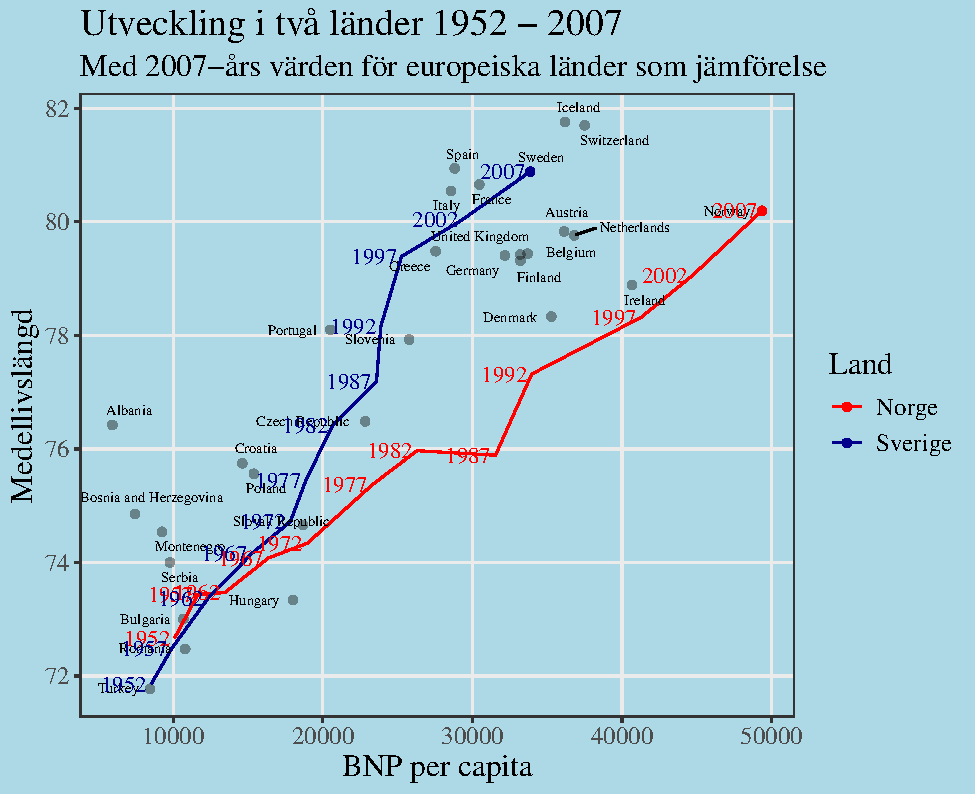
\includegraphics{R-anvisningar_files/figure-latex/unnamed-chunk-54-1} \end{center}

\begin{exercise}[Dekonstruera grafen]
Vilka geografiska former (punkter, linjer ytor) visas i grafen och hur är de kopplade till datans variabler? Vilka ändringar har gjorts från standardtemat (bakgrundsfärg, typsnitt, teckenstorlek)?
\end{exercise}

\begin{exercise}[Rekonstrera grafen]
Använd en chatbot (såsom Microsofts co-pilot eller OpenAIs ChatGPT) för att rekonstrera grafen. Börja med att beskriva grafen i ord och be om R-kod. Klipp ut koden och kör i R. Läs koden du fått. Finns det några delar som är svåra att förstå. Med vissa chatverktyg kan man också klippa in bilden och be om den bakomliggande koden.
\end{exercise}

\begin{exercise}[Steg i Excel]
Hur skulle man gå tillväga för att skapa samma graf i Excel? Be en chatbot om en stegvis instruktion.
\end{exercise}

\chapter{Beskrivande statistik}\label{beskrivande-statistik}

Datorövning 2 handlar om beräkning av beskrivande statistik i R. Efter övningen ska vi kunna

\begin{itemize}
\tightlist
\item
  Importera data från en excelfil,
\item
  Beräkna lämpliga lägesmått för en variabel,
\item
  Beräkna lämpliga spridningsmått för en variabel,
\item
  Konstruera grafer som jämför två eller flera gruppers läge och spridning.
\end{itemize}

\section{Repetition från datorövning 1}\label{repetition-fruxe5n-datoruxf6vning-1}

När man arbetar i R är det klokt att använda ett avancerat gränssnitt som RStudio och att skriva sin kod i ett separat skript. I RStudio kan man starta ett nytt skript genom \emph{Ctrl + Shift + N}.

Mycket funktionalitet i R ligger i tilläggspaket (\emph{Packages}). Paket måste installeras första gången de används och laddas varje session de används, t.ex.

\begin{Shaded}
\begin{Highlighting}[]
\CommentTok{\# install.packages("tidyverse") \# Installera tidyverse}
\FunctionTok{library}\NormalTok{(tidyverse)              }\CommentTok{\# Ladda ett paket}
\end{Highlighting}
\end{Shaded}

Objekt skapas med \emph{assign}-pilen \texttt{\textless{}-}. Det är ett sätt att importera data till R. Det är dock vanligare importera från en extern fil. Mer om det senare.

Vi arbetar nästan alltid med data på tabellformat där variablerna är kolumner och observationerna rader. I gapminder-datan ges raderna av ett land för ett visst år.

\begin{Shaded}
\begin{Highlighting}[]
\FunctionTok{library}\NormalTok{(gapminder)}
\NormalTok{gapminder                       }\CommentTok{\# Skriv ut objektet gapminder}
\end{Highlighting}
\end{Shaded}

Funktioner agerar på objekt och ger något utfall. Här beräknas medeltempot med funktionen \texttt{mean()}. Dollartecknet används för att ange en specifik kolumn i dataobjektet. Funktioner styrs av möjliga argument - här används \texttt{na.rm} för att ange att saknade värden inte ska tas med i beräkningen

\begin{Shaded}
\begin{Highlighting}[]
\FunctionTok{mean}\NormalTok{(gapminder}\SpecialCharTok{$}\NormalTok{lifeExp, }\AttributeTok{na.rm =}\NormalTok{ T) }\CommentTok{\# Beräkna medel av lifeExp}
\end{Highlighting}
\end{Shaded}

\begin{verbatim}
## [1] 59.47444
\end{verbatim}

Funktionerna \texttt{filter()} och \texttt{select()} kan användas för att välja kolumner och rader. Funktioner kan länkas samman med en pipe \texttt{\%\textgreater{}\%} för att skapa sekvenser av funktioner. Man kan tänka på pipen som \emph{och sen}.

\begin{Shaded}
\begin{Highlighting}[]
\NormalTok{gapminder }\SpecialCharTok{\%\textgreater{}\%}
  \FunctionTok{filter}\NormalTok{(country }\SpecialCharTok{==} \StringTok{"Norway"}\NormalTok{, year }\SpecialCharTok{\textgreater{}} \DecValTok{1972}\NormalTok{) }\SpecialCharTok{\%\textgreater{}\%}
  \FunctionTok{select}\NormalTok{(country, lifeExp)}
\end{Highlighting}
\end{Shaded}

Slutligen tittade vi på grafer med ggplot2-paketet. En ggplot byggs upp med tre grundelar: data, geometrier (grafens objekt och former), och \emph{aesthetics} (utseende och placering av geometrierna). I ett enkelt spridningsdiagram är data två numeriska variabler, geometrierna är punkter, och punkternas placering ges av en x-koordinat och en y-koordinat. Ytterligare \emph{aesthetics} kan vara punkternas färger (\texttt{color}) och storlek (\texttt{size}).

\begin{Shaded}
\begin{Highlighting}[]
\NormalTok{dat\_small }\OtherTok{\textless{}{-}}\NormalTok{ gapminder }\SpecialCharTok{\%\textgreater{}\%} \FunctionTok{filter}\NormalTok{(year }\SpecialCharTok{==} \DecValTok{2007}\NormalTok{)}
\FunctionTok{ggplot}\NormalTok{(dat\_small, }\FunctionTok{aes}\NormalTok{(gdpPercap, lifeExp, }
                      \AttributeTok{size =}\NormalTok{ pop, }\AttributeTok{color =}\NormalTok{ continent)) }\SpecialCharTok{+}
  \FunctionTok{geom\_point}\NormalTok{()}
\end{Highlighting}
\end{Shaded}

\section{Import av data från en Excelfil}\label{import-av-data-fruxe5n-en-excelfil}

Inom vetenskapen är Excel det vanligaste filformatet för mindre datamängder. Till den här delen ska vi återigen arbeta med data från \emph{Gapminder}.

\begin{exercise}[Excelfil från Canvas]
Hitta excelfilen \emph{Gapminder.xlsx} på Canvas och ladda ner den. Hitta mappen som filen laddats ned till.
\end{exercise}

I R kan man läsa in data från en Excel-fil med funktionen \texttt{read\_excel()} från paketet \texttt{readxl}. Som argument till funktionen sätts filens sökväg - dess placering på hårddisken. Stycket nedan importerar från en excelfil som ligger på hårddisken \emph{C:} i mappen \emph{Downloads}, under \emph{User\_name}, under \emph{Users}.

\begin{Shaded}
\begin{Highlighting}[]
\FunctionTok{library}\NormalTok{(readxl)  }\CommentTok{\# Ladda readxl}
\end{Highlighting}
\end{Shaded}

\begin{Shaded}
\begin{Highlighting}[]
\NormalTok{gapminder }\OtherTok{\textless{}{-}} \FunctionTok{read\_excel}\NormalTok{(}\StringTok{"C:/Users/Name/Downloads/Gapminder.xlsx"}\NormalTok{)}
\CommentTok{\# Läs in från en lokal excelfil}
\NormalTok{gapminder}
\end{Highlighting}
\end{Shaded}

\begin{exercise}[Importera från excelfil]
Var ligger den nedladdade filen \emph{Gapminder.xlsx}? Gör lämplig ändring i koden ovan för att läsa in data från den filen. Notera att R använder högerlutande snedstreck \texttt{/}, så om en kopierad sökväg har vänster-snedstreck måste de ändras. Kontrollera att datan blivit korrekt inläst genom att köra objektnamnet \texttt{gapminder}.
\end{exercise}

En R-session har alltid en grundmapp, ett \emph{Working directory}. Man kan se vilken mapp det är genom att köra

\begin{Shaded}
\begin{Highlighting}[]
\FunctionTok{getwd}\NormalTok{() }\CommentTok{\# Ange working directory}
\end{Highlighting}
\end{Shaded}

En filsökväg kan anges antingen som en fullständig sökväg, som ovan, eller relativt \emph{working directory}. Om man till exempel har en fil \emph{Gapminder.xlsx} som ligger i en mapp \emph{Data} som i sin tur ligger i \emph{working directory}, kan man importera data från filen med

\begin{Shaded}
\begin{Highlighting}[]
\NormalTok{gapminder }\OtherTok{\textless{}{-}} \FunctionTok{read\_excel}\NormalTok{(}\StringTok{"Data/Gapminder.xlsx"}\NormalTok{)}
\CommentTok{\# Läs in från en lokal excelfil (relativt wd)}
\NormalTok{gapminder }
\end{Highlighting}
\end{Shaded}

\begin{exercise}[Working directory]
Identifiera \emph{working directory} för din nuvarande Rs-session genom att köra \texttt{getwd()}.
\end{exercise}

RStudio har också en inbyggd funktionalitet för att importera data. Man kan hitta den genom att gå till \emph{Environment}-fliken och sedan \emph{Import Dataset}. Det kan vara en bra hjälp, i synnerhet om man vill sätta datatyp för någon specifik kolumn.

Om du inte har tillgång till Canvas kan Gapminder-datan alternativt hämtas från paketet Gapminder.

\begin{Shaded}
\begin{Highlighting}[]
\CommentTok{\# install.packages("gapminder")}
\FunctionTok{library}\NormalTok{(gapminder)             }
\NormalTok{gapminder                      }
\end{Highlighting}
\end{Shaded}

\section{\texorpdfstring{Ändra och skapa nya kolumner med \texttt{mutate}}{Ändra och skapa nya kolumner med mutate}}\label{uxe4ndra-och-skapa-nya-kolumner-med-mutate}

Variabler kan omräknas och nya variabler kan skapas med \texttt{mutate}-funktionen. I gapminder-datan finns bnp per capita. Om man vill ha nationell BNP kan man skapa en ny kolumn och beräkna den som bnp per capita gånger populationen.

\begin{Shaded}
\begin{Highlighting}[]
\NormalTok{gapminder }\OtherTok{\textless{}{-}}\NormalTok{ gapminder }\SpecialCharTok{\%\textgreater{}\%}             \CommentTok{\# Ta datan, och sen}
  \FunctionTok{mutate}\NormalTok{(}\AttributeTok{gdp =}\NormalTok{ gdpPercap }\SpecialCharTok{*}\NormalTok{ pop)        }\CommentTok{\# Beräkna bnp}
\end{Highlighting}
\end{Shaded}

Den inledande delen med \texttt{gapminder\ \textless{}-} gör så att utfallet av beräkningen sparas i objektet \texttt{gapminder}.
Vi kan skriva ut objektet och se resultatet av beräkningen:

\begin{Shaded}
\begin{Highlighting}[]
\NormalTok{gapminder}
\end{Highlighting}
\end{Shaded}

Om man vill skapa en kolumn med mellanrum i namnet måste man skriva namnet inom \emph{backticks} ` för att ange att namnet ska tolkas som en enhet. Jag rekommenderar att undvika mellanrum i kolumnnamn och istället använda stora bokstäver eller understreck för ett nytt ord (\texttt{NationalGDP} eller \texttt{National\_GDP}).

\begin{Shaded}
\begin{Highlighting}[]
\NormalTok{gapminder }\SpecialCharTok{\%\textgreater{}\%} 
  \FunctionTok{mutate}\NormalTok{(}\StringTok{\textasciigrave{}}\AttributeTok{National GDP}\StringTok{\textasciigrave{}} \OtherTok{=}\NormalTok{ gdpPercap }\SpecialCharTok{*}\NormalTok{ pop)}
\end{Highlighting}
\end{Shaded}

\section{Sammanfattande lägesmått}\label{sammanfattande-luxe4gesmuxe5tt}

Den importerade datan anger medellivslängd, populationsstorlek och bnp per capita per land och år. Vi kan börja med att producera en bubbelgraf över datan - en av de presentationer Gapminder ofta använder. En bubbelgraf är ett spridningsdiagram där punktens storlek beror på en tredje variabel.

\begin{Shaded}
\begin{Highlighting}[]
\FunctionTok{ggplot}\NormalTok{(gapminder, }\FunctionTok{aes}\NormalTok{(gdpPercap, lifeExp, }
                      \AttributeTok{size =}\NormalTok{ pop, }\AttributeTok{color =}\NormalTok{ continent)) }\SpecialCharTok{+}
  \FunctionTok{geom\_point}\NormalTok{() }\SpecialCharTok{+}
  \FunctionTok{facet\_wrap}\NormalTok{(}\SpecialCharTok{\textasciitilde{}}\NormalTok{ year)}
\end{Highlighting}
\end{Shaded}

En interaktiv version kan vara bra om man vill identifiera någon specifik punkt.

\begin{Shaded}
\begin{Highlighting}[]
\NormalTok{g }\OtherTok{\textless{}{-}} \FunctionTok{ggplot}\NormalTok{(gapminder, }\FunctionTok{aes}\NormalTok{(gdpPercap, lifeExp, }\AttributeTok{size =}\NormalTok{ pop, }
                           \AttributeTok{color =}\NormalTok{ continent, }\AttributeTok{text =}\NormalTok{ country)) }\SpecialCharTok{+}
  \FunctionTok{geom\_point}\NormalTok{() }\SpecialCharTok{+}
  \FunctionTok{facet\_wrap}\NormalTok{(}\SpecialCharTok{\textasciitilde{}}\NormalTok{ year)}

\CommentTok{\# install.packages("plotly")}
\FunctionTok{library}\NormalTok{(plotly)                        }\CommentTok{\# Ladda paketet plotly}
\FunctionTok{ggplotly}\NormalTok{(g)                            }\CommentTok{\# Interaktiv graf g}
\end{Highlighting}
\end{Shaded}

Under föreläsningen såg vi exempel på två lägesmått: medelvärdet (egentligen det \emph{aritmetiska} medelvärdet) och medianen. De har bägge enkla funktioner i R: \texttt{mean()} respektive \texttt{median()}. Vi plockar ut en variabel ur datan och beräknar bägge.

\begin{Shaded}
\begin{Highlighting}[]
\NormalTok{gdpPercap }\OtherTok{\textless{}{-}}\NormalTok{ gapminder}\SpecialCharTok{$}\NormalTok{gdpPercap }\CommentTok{\# Skapa en vektor gdpPercap}
\FunctionTok{mean}\NormalTok{(gdpPercap)                  }\CommentTok{\# Beräkna medelvärdet}
\end{Highlighting}
\end{Shaded}

\begin{verbatim}
## [1] 7215.327
\end{verbatim}

\begin{Shaded}
\begin{Highlighting}[]
\FunctionTok{median}\NormalTok{(gdpPercap)                }\CommentTok{\# Beräkna medianen}
\end{Highlighting}
\end{Shaded}

\begin{verbatim}
## [1] 3531.847
\end{verbatim}

Samma sak kan göras med en pipe \texttt{\%\textgreater{}\%} och \texttt{summarise()}.

\begin{Shaded}
\begin{Highlighting}[]
\NormalTok{gapminder }\SpecialCharTok{\%\textgreater{}\%}
  \FunctionTok{summarise}\NormalTok{(}\AttributeTok{Mean =} \FunctionTok{mean}\NormalTok{(gdpPercap),}
            \AttributeTok{Median =} \FunctionTok{median}\NormalTok{(gdpPercap))}
\end{Highlighting}
\end{Shaded}

\begin{exercise}[Lägesmått av livslängd]
Gör lämpliga ändringar i exemplet ovan för att beräkna lägesmått för medellivslängd (\texttt{lifeExp}).
\end{exercise}

Den andra lösningen, med en pipe och \texttt{summarise()}, kan enkelt utvecklas med ett \texttt{group\_by()}-steg för att beräkna medel och median per någon grupp, t.ex. per år.

\begin{Shaded}
\begin{Highlighting}[]
\NormalTok{gapminder }\SpecialCharTok{\%\textgreater{}\%}                           \CommentTok{\# Ta datan, och sen}
  \FunctionTok{group\_by}\NormalTok{(year) }\SpecialCharTok{\%\textgreater{}\%}                    \CommentTok{\# gruppera efter år, och}
  \FunctionTok{summarise}\NormalTok{(}\AttributeTok{Mean =} \FunctionTok{mean}\NormalTok{(gdpPercap),     }\CommentTok{\# beräkna medelvärde och}
            \AttributeTok{Median =} \FunctionTok{median}\NormalTok{(gdpPercap)) }\CommentTok{\# medianen av gdpPercap}
\end{Highlighting}
\end{Shaded}

\begin{exercise}[Lägesmått per kontinent]
Gör lämpliga ändringar i exemplet ovan för att beräkna lägesmått per kontinent. Vad måste läggas till för att också beräkna maximum och minimum per kontinent (funktionerna \texttt{max()} och \texttt{min()})?
\end{exercise}

\begin{exercise}[Upprepade mätningar]
Finns det några problem med att beräkna medelvärde per kontinent på den här datan?
\end{exercise}

I vetenskapliga publikationer redovisas medelvärden ofta med ett stapeldiagram. Som exempel ges staplar för medelvärdet av bnp per kontinent för 2007.

\begin{Shaded}
\begin{Highlighting}[]
\NormalTok{dat\_gdp\_2007 }\OtherTok{\textless{}{-}}\NormalTok{ gapminder }\SpecialCharTok{\%\textgreater{}\%}       \CommentTok{\# Ta datan, och sen}
  \FunctionTok{filter}\NormalTok{(year }\SpecialCharTok{==} \DecValTok{2007}\NormalTok{) }\SpecialCharTok{\%\textgreater{}\%}          \CommentTok{\# filtrera för 2007, och sen}
  \FunctionTok{group\_by}\NormalTok{(continent) }\SpecialCharTok{\%\textgreater{}\%}           \CommentTok{\# gruppera kontinenter, och}
  \FunctionTok{summarise}\NormalTok{(}\AttributeTok{Mean =} \FunctionTok{mean}\NormalTok{(gdpPercap)) }\CommentTok{\# summera med medelvärdet}

\FunctionTok{ggplot}\NormalTok{(dat\_gdp\_2007, }\FunctionTok{aes}\NormalTok{(continent, Mean)) }\SpecialCharTok{+}
  \FunctionTok{geom\_col}\NormalTok{()                  }\CommentTok{\# Illustrera med kolumner (columns)}
\end{Highlighting}
\end{Shaded}

\begin{exercise}[Graf för livslängd]
Gör om stapeldiagrammet. Denna gång med livslängd (\texttt{lifeExp}) istället för bnp per capita (\texttt{gdpPercap}).
\end{exercise}

\section{Sammanfattande spridningsmått}\label{sammanfattande-spridningsmuxe5tt}

Under föreläsningarna såg vi några mått på spridning: varians, standardavvikelse och kvartilavstånd (IQR, \emph{inter-quartile range}). De har alla motsvarande funktioner i R (\texttt{var()}, \texttt{sd()}, och \texttt{IQR()}) som kan användas på samma sätt som funktionerna för lägesmått.

\begin{Shaded}
\begin{Highlighting}[]
\NormalTok{gdpPercap }\OtherTok{\textless{}{-}}\NormalTok{ gapminder}\SpecialCharTok{$}\NormalTok{gdpPercap }\CommentTok{\# Skapa en vektor gdpPercap}

\FunctionTok{var}\NormalTok{(gdpPercap)                   }\CommentTok{\# Beräkna varians}
\FunctionTok{sd}\NormalTok{(gdpPercap)                    }\CommentTok{\# Beräkna standardavvikelse}
\FunctionTok{IQR}\NormalTok{(gdpPercap)                   }\CommentTok{\# Beräkna kvartilavstånd}
\end{Highlighting}
\end{Shaded}

Alternativt med en pipe och \texttt{summarise()}.

\begin{Shaded}
\begin{Highlighting}[]
\NormalTok{gapminder }\SpecialCharTok{\%\textgreater{}\%}                       \CommentTok{\# Ta datan, och}
  \FunctionTok{summarise}\NormalTok{(}\AttributeTok{Var =} \FunctionTok{var}\NormalTok{(gdpPercap),   }\CommentTok{\# beräkna varians,}
            \AttributeTok{Sd =} \FunctionTok{sd}\NormalTok{(gdpPercap),     }\CommentTok{\# standardavvikelse,}
            \AttributeTok{IQR =} \FunctionTok{IQR}\NormalTok{(gdpPercap))   }\CommentTok{\# och kvartilavstånd}
\end{Highlighting}
\end{Shaded}

Lösningen med pipe och \texttt{summarise()} kan som tidigare utvecklas med \texttt{group\_by()}.

\begin{Shaded}
\begin{Highlighting}[]
\NormalTok{gapminder }\SpecialCharTok{\%\textgreater{}\%}
  \FunctionTok{group\_by}\NormalTok{(year) }\SpecialCharTok{\%\textgreater{}\%}
  \FunctionTok{summarise}\NormalTok{(}\AttributeTok{Varians =} \FunctionTok{var}\NormalTok{(gdpPercap),}
            \AttributeTok{Standardavvikelse =} \FunctionTok{sd}\NormalTok{(gdpPercap),}
\NormalTok{            Kvartilavstånd }\OtherTok{=} \FunctionTok{IQR}\NormalTok{(gdpPercap))}
\end{Highlighting}
\end{Shaded}

\begin{exercise}[Graf för livslängd]
Gör lämpliga ändringar i det sista exempel för att istället beräkna spridningsmått för livslängd.
\end{exercise}

Vi avslutar med tre vanliga illustrationer av vetenskaplig data - ett linjediagram med felstaplar, ett stapeldiagram med felstaplar, och ett lådagram. För linjediagrammet beräknar vi medelvärdet och spridningsmått för bnp över år och kontinent. Som spridningsmått använder vi \emph{medelfelet}, vilket beräknas som standardavvikelse delat på roten ur antalet observationer.

\begin{Shaded}
\begin{Highlighting}[]
\NormalTok{dat\_sum }\OtherTok{\textless{}{-}}\NormalTok{ gapminder }\SpecialCharTok{\%\textgreater{}\%}
  \FunctionTok{group\_by}\NormalTok{(year, continent) }\SpecialCharTok{\%\textgreater{}\%}
  \FunctionTok{summarise}\NormalTok{(}\AttributeTok{Mean =} \FunctionTok{mean}\NormalTok{(gdpPercap),}
            \AttributeTok{SE =} \FunctionTok{sd}\NormalTok{(gdpPercap) }\SpecialCharTok{/} \FunctionTok{sqrt}\NormalTok{(}\FunctionTok{n}\NormalTok{()))}
\NormalTok{dat\_sum}
\end{Highlighting}
\end{Shaded}

Med \texttt{ggplot2} kan vi bygga ett linjediagram med \texttt{geom\_line()} och lägga till felstaplar med \texttt{geom\_errorbar()}. Den senare behöver \texttt{aes()}-argument för \texttt{ymin} och \texttt{ymax} - nedre och övre del av felstapeln. Vi sätter dem till medelvärdet minus respektive plus ett medelfel.

\begin{Shaded}
\begin{Highlighting}[]
\FunctionTok{ggplot}\NormalTok{(dat\_sum, }\FunctionTok{aes}\NormalTok{(year, Mean, }\AttributeTok{color =}\NormalTok{ continent)) }\SpecialCharTok{+}
  \FunctionTok{geom\_line}\NormalTok{() }\SpecialCharTok{+}
  \FunctionTok{geom\_errorbar}\NormalTok{(}\FunctionTok{aes}\NormalTok{(}\AttributeTok{ymin =}\NormalTok{ Mean }\SpecialCharTok{{-}}\NormalTok{ SE, }\AttributeTok{ymax =}\NormalTok{ Mean }\SpecialCharTok{+}\NormalTok{ SE))}
\end{Highlighting}
\end{Shaded}

\begin{exercise}[Bredd]
Felstaplarna från \texttt{geom\_errorbar()} har väldigt breda ändar. Använd hjälpsidan för geomet \texttt{?geom\_errorbar}, i synnerhet exemplen längst ned, och se om det går att ändra bredden.
\end{exercise}

En graf med staplar och felstaplar kan konstrueras på ett liknande sätt. Följande exempel visar staplar över livslängd per kontinent. Felstapeln ges av standardavvikelsen.

\begin{Shaded}
\begin{Highlighting}[]
\NormalTok{dat\_sum }\OtherTok{\textless{}{-}}\NormalTok{ gapminder }\SpecialCharTok{\%\textgreater{}\%}          \CommentTok{\# Ta datan, och sen}
  \FunctionTok{filter}\NormalTok{(year }\SpecialCharTok{==} \DecValTok{2007}\NormalTok{) }\SpecialCharTok{\%\textgreater{}\%}        \CommentTok{\# filtrera på år, och sen}
  \FunctionTok{group\_by}\NormalTok{(continent) }\SpecialCharTok{\%\textgreater{}\%}         \CommentTok{\# gruppera efter kontinent,}
  \FunctionTok{summarise}\NormalTok{(}\AttributeTok{Mean =} \FunctionTok{mean}\NormalTok{(lifeExp), }\CommentTok{\# summera med medelvärde,}
            \AttributeTok{SD =} \FunctionTok{sd}\NormalTok{(lifeExp))     }\CommentTok{\# och standardavvikelse}
\NormalTok{dat\_sum}
\end{Highlighting}
\end{Shaded}

Vi bygger en ggplot med \texttt{geom\_col()} och \texttt{geom\_errorbar()}. Felstapels konstruktion kan anges i en notis med funktionen \texttt{labs()}.

\begin{Shaded}
\begin{Highlighting}[]
\FunctionTok{ggplot}\NormalTok{(dat\_sum, }\FunctionTok{aes}\NormalTok{(continent, Mean, }\AttributeTok{fill =}\NormalTok{ continent)) }\SpecialCharTok{+}
  \FunctionTok{geom\_col}\NormalTok{()}\SpecialCharTok{+}                                            
  \FunctionTok{geom\_errorbar}\NormalTok{(}\FunctionTok{aes}\NormalTok{(}\AttributeTok{ymin =}\NormalTok{ Mean }\SpecialCharTok{{-}}\NormalTok{ SD, }\AttributeTok{ymax =}\NormalTok{ Mean }\SpecialCharTok{+}\NormalTok{ SD)) }\SpecialCharTok{+}
  \FunctionTok{labs}\NormalTok{(}\AttributeTok{title =} \StringTok{"Average life expectancy by continent, 2007"}\NormalTok{,}
       \AttributeTok{caption =} \StringTok{"Errorbars given by mean +/{-} standard deviation.}
\StringTok{       Source: Gapminder"}\NormalTok{)}
\end{Highlighting}
\end{Shaded}

\begin{exercise}[Staplar för 1982]
Gör lämpliga ändringar i exempel ovan för att konstruera ett stapeldiagram med felstaplar för året 1982 och variabeln gdpPercap.
\end{exercise}

Ett lådagram anger fördelningen av en variabel genom att illustrera minimum, maximum och kvartiler. Kvartiler är mått som delar en datamängd i fyra lika stora delar (så att en fjärdedel ligger under första kvartilen, en fjärdedel mellan första och andra kvartil, och så vidare). Med \texttt{ggplot2} kan vi bygga ett lådagram med \texttt{geom\_boxplot()}. Exempel ger en låda per år och kontinent.

\begin{Shaded}
\begin{Highlighting}[]
\FunctionTok{ggplot}\NormalTok{(gapminder, }\FunctionTok{aes}\NormalTok{(year, lifeExp, }\AttributeTok{fill =}\NormalTok{ continent, }
                      \AttributeTok{group =}\NormalTok{ year)) }\SpecialCharTok{+}
  \FunctionTok{geom\_boxplot}\NormalTok{() }\SpecialCharTok{+}                                                     
  \FunctionTok{facet\_wrap}\NormalTok{(}\SpecialCharTok{\textasciitilde{}}\NormalTok{ continent)                                              }
\end{Highlighting}
\end{Shaded}

\begin{exercise}[Group-argumentet]
I lådagrammet används argumentet \texttt{group}. Vad gör det? Vad händer om man tar bort det?
\end{exercise}

Om man vill ha med både data på observationsnivån och summerad data i en graf kan man ange olika data till olika geom. Vi kan t.ex. lägga till en markör för medelvärdet i en boxplot.

\begin{Shaded}
\begin{Highlighting}[]
\NormalTok{gapminder\_2007 }\OtherTok{\textless{}{-}}\NormalTok{ gapminder }\SpecialCharTok{\%\textgreater{}\%} \FunctionTok{filter}\NormalTok{(year }\SpecialCharTok{==} \DecValTok{2007}\NormalTok{)}
\NormalTok{gapminder\_agg }\OtherTok{\textless{}{-}}\NormalTok{ gapminder\_2007 }\SpecialCharTok{\%\textgreater{}\%} 
  \FunctionTok{group\_by}\NormalTok{(continent) }\SpecialCharTok{\%\textgreater{}\%} 
  \FunctionTok{summarise}\NormalTok{(}\AttributeTok{lifeExp =} \FunctionTok{mean}\NormalTok{(lifeExp))}
\NormalTok{gapminder\_agg}

\FunctionTok{ggplot}\NormalTok{() }\SpecialCharTok{+}
  \FunctionTok{geom\_boxplot}\NormalTok{(}\FunctionTok{aes}\NormalTok{(lifeExp, continent), }\AttributeTok{data =}\NormalTok{ gapminder\_2007) }\SpecialCharTok{+}
  \FunctionTok{geom\_point}\NormalTok{(}\FunctionTok{aes}\NormalTok{(lifeExp, continent), }\AttributeTok{data =}\NormalTok{ gapminder\_agg, }
             \AttributeTok{color =} \StringTok{"red"}\NormalTok{, }\AttributeTok{shape =} \StringTok{"X"}\NormalTok{, }\AttributeTok{size =} \DecValTok{6}\NormalTok{)}
\end{Highlighting}
\end{Shaded}

Här byggs boxarna med datan \texttt{gapminder} och punkterna med den aggregerade datan.

\section{Ordna upp beskrivande statistik och exportera}\label{ordna-upp-beskrivande-statistik-och-exportera}

Efter att ha beräknat någon beskrivande statistik kan det vara bra att titta på hur resultaten kan snyggas upp och exporteras i något lämpligt format. Ta den tabell med medelvärden vi producerade i ett tidigare exempel.

\begin{Shaded}
\begin{Highlighting}[]
\NormalTok{dat\_sum }\OtherTok{\textless{}{-}}\NormalTok{ gapminder }\SpecialCharTok{\%\textgreater{}\%}          \CommentTok{\# Ta datan, och sen}
  \FunctionTok{filter}\NormalTok{(year }\SpecialCharTok{==} \DecValTok{2007}\NormalTok{) }\SpecialCharTok{\%\textgreater{}\%}        \CommentTok{\# filtrera på år, och sen}
  \FunctionTok{group\_by}\NormalTok{(continent) }\SpecialCharTok{\%\textgreater{}\%}         \CommentTok{\# gruppera efter kontinent,}
  \FunctionTok{summarise}\NormalTok{(}\AttributeTok{Mean =} \FunctionTok{mean}\NormalTok{(lifeExp), }\CommentTok{\# summera med medelvärde,}
            \AttributeTok{SD =} \FunctionTok{sd}\NormalTok{(lifeExp))     }\CommentTok{\# och standardavvikelse}
\NormalTok{dat\_sum}
\end{Highlighting}
\end{Shaded}

Objekt kan exporteras från R på liknande som det importeras - med särskilda exportfunktioner (\emph{write}-funktioner) beroende på filtyp. För att exportera till en csv-fil man man använda \texttt{write\_csv()}. Ingående argument är det objekt man vill exportera och den fil man vill exportera till. R ger ingen varning om man skriver över en existerande fil, så var lite försiktiga här.

Precis som vid import använder R \emph{working directory} om inget annat anges. Följande exporterar objektet \texttt{dat\_sum} till en csv-fil \emph{Exporterad data från R.csv} i \emph{working directory}.

\begin{Shaded}
\begin{Highlighting}[]
\FunctionTok{getwd}\NormalTok{()                          }\CommentTok{\# Se nuvarande working directory}
\FunctionTok{write\_csv}\NormalTok{(dat\_sum, }\StringTok{"Exporterad data från R.csv"}\NormalTok{) }\CommentTok{\# Exportera data}
\end{Highlighting}
\end{Shaded}

Därifrån skulle man kunna öppna filen i något kalkylprogram, snygga till layouten, och sedan klippa in i ett textdokument.

\section{Kumulativt medelvärde}\label{kumulativt-medelvuxe4rde}

Om man har data som av någon anledning samlas in i sekvens kan det vara intressant att beräkna och illustrera den med ett \emph{kumulativt medelvärde}. En serie med kumulativa medelvärden beräknas genom att för varje nytt värde ta medelvärden av de värden man hittills samlat in - vid tio värden tar man medelvärdet av de tio, vid elva värden medelvärdet av de elva, och så vidare.

Med de tärningsvärden vi hade innan kan vi beräkna ett kumulativt medelvärde genom att först beräkna summan med \texttt{cumsum()} och sedan dela på antalet kast. För att förenkla beräkningen av antalen tar vi fram sekvensen med antal kast i ett \texttt{mutate()}-steg.

\begin{Shaded}
\begin{Highlighting}[]
\NormalTok{dat\_dice }\OtherTok{\textless{}{-}} \FunctionTok{data.frame}\NormalTok{(}\AttributeTok{Utfall =} \FunctionTok{c}\NormalTok{(}\DecValTok{6}\NormalTok{,}\DecValTok{3}\NormalTok{,}\DecValTok{2}\NormalTok{,}\DecValTok{3}\NormalTok{,}\DecValTok{5}\NormalTok{)) }\SpecialCharTok{\%\textgreater{}\%}
  \FunctionTok{mutate}\NormalTok{(}\AttributeTok{Kast =} \DecValTok{1}\SpecialCharTok{:}\FunctionTok{n}\NormalTok{())                           }
\NormalTok{dat\_dice}

\NormalTok{dat\_dice }\OtherTok{\textless{}{-}}\NormalTok{ dat\_dice }\SpecialCharTok{\%\textgreater{}\%}
  \FunctionTok{mutate}\NormalTok{(}\AttributeTok{kumulativ\_summa =} \FunctionTok{cumsum}\NormalTok{(Utfall),  }
\NormalTok{         kumulativt\_medelvärde }\OtherTok{=}\NormalTok{ kumulativ\_summa }\SpecialCharTok{/}\NormalTok{ Kast)}
\NormalTok{dat\_dice}
\end{Highlighting}
\end{Shaded}

Om beräkning inte är uppenbar här, ta någon minut för att förstå den.

\begin{exercise}[Kumulativt medelvärde]

Vad ska läggas till för att stycket nedan ska ge en linjegraf över medelvärdet?

\begin{Shaded}
\begin{Highlighting}[]
\FunctionTok{ggplot}\NormalTok{(dat\_dice, }\FunctionTok{aes}\NormalTok{(}\AttributeTok{x =}\NormalTok{ Kast, }\AttributeTok{y =}\NormalTok{ \_\_\_)) }\SpecialCharTok{+}
  \FunctionTok{\_\_\_}\NormalTok{()}
\end{Highlighting}
\end{Shaded}

\end{exercise}

\begin{exercise}[Fler tärningskast]

Kasta din tärning ytterligare några gånger, gärna på en mjuk yta. Fyll i dina utfall och gör grafen från föregående uppgift. Kan man se en tendens för medelvärdet att minska i varians vid fler kast?

\begin{Shaded}
\begin{Highlighting}[]
\NormalTok{dat\_dice }\OtherTok{\textless{}{-}} \FunctionTok{data.frame}\NormalTok{(}\AttributeTok{Utfall =} \FunctionTok{c}\NormalTok{(\_\_\_)) }\SpecialCharTok{\%\textgreater{}\%} 
  \FunctionTok{mutate}\NormalTok{(}\AttributeTok{Kast =} \DecValTok{1}\SpecialCharTok{:}\FunctionTok{n}\NormalTok{(),                                 }
         \StringTok{\textasciigrave{}}\AttributeTok{Kumulativ summa}\StringTok{\textasciigrave{}} \OtherTok{=} \FunctionTok{cumsum}\NormalTok{(Utfall),           }
         \StringTok{\textasciigrave{}}\AttributeTok{Kumulativt medelvärde}\StringTok{\textasciigrave{}} \OtherTok{=} \StringTok{\textasciigrave{}}\AttributeTok{Kumulativ summa}\StringTok{\textasciigrave{}} \SpecialCharTok{/}\NormalTok{ Kast)}
\NormalTok{dat\_dice}
\end{Highlighting}
\end{Shaded}

\end{exercise}

\begin{exercise}[Kumulativ frekvens]

Om man vill titta på andelen gånger ett visst utfall inträffat talar man om \emph{kumulativ frekvens} snarare än \emph{kumulativt medelvärde}. Använd stycket nedan för att titta på andelen gånger utfallet varit en etta (ett \emph{positivt} utfall, i begreppets kliniska mening). Om ett inte är ett möjligt utfall på din tärning, ändra ettan till något mer lämpligt.

\begin{Shaded}
\begin{Highlighting}[]
\NormalTok{dat\_dice }\OtherTok{\textless{}{-}} \FunctionTok{data.frame}\NormalTok{(}\AttributeTok{Utfall =} \FunctionTok{c}\NormalTok{(\_\_\_)) }\SpecialCharTok{\%\textgreater{}\%} 
  \FunctionTok{mutate}\NormalTok{(}\AttributeTok{Kast =} \DecValTok{1}\SpecialCharTok{:}\FunctionTok{n}\NormalTok{(),}
         \AttributeTok{positivt\_utfall =}\NormalTok{ Utfall }\SpecialCharTok{==} \DecValTok{1}\NormalTok{,              }
         \AttributeTok{kumulativt\_antal =} \FunctionTok{cumsum}\NormalTok{(positivt\_utfall),}
         \AttributeTok{kumulativ\_frekvens =}\NormalTok{ kumulativt\_antal }\SpecialCharTok{/}\NormalTok{ Kast)}
\NormalTok{dat\_dice}

\FunctionTok{ggplot}\NormalTok{(dat\_dice, }\FunctionTok{aes}\NormalTok{(}\AttributeTok{x =}\NormalTok{ Kast, }\AttributeTok{y =}\NormalTok{ kumulativ\_frekvens)) }\SpecialCharTok{+}
  \FunctionTok{geom\_line}\NormalTok{()}
\end{Highlighting}
\end{Shaded}

\end{exercise}

\section{\texorpdfstring{Bonus. Tredimensionella grafer med \texttt{plotly}}{Bonus. Tredimensionella grafer med plotly}}\label{bonus.-tredimensionella-grafer-med-plotly}

Paketet \texttt{plotly} kan användas för att göra interaktiva graf och grafer med tre dimensioner. Börja med att ladda paketet.

\begin{Shaded}
\begin{Highlighting}[]
\FunctionTok{library}\NormalTok{(plotly)}
\end{Highlighting}
\end{Shaded}

Vi börjar med ett enkelt exempel på en 3d-graf med lite skapad data.

\begin{Shaded}
\begin{Highlighting}[]
\NormalTok{dat\_ex }\OtherTok{\textless{}{-}} \FunctionTok{data.frame}\NormalTok{(}\AttributeTok{Var1 =} \FunctionTok{c}\NormalTok{(}\DecValTok{1}\NormalTok{,}\DecValTok{2}\NormalTok{,}\DecValTok{3}\NormalTok{), }\AttributeTok{Var2 =} \FunctionTok{c}\NormalTok{(}\DecValTok{3}\NormalTok{,}\DecValTok{1}\NormalTok{,}\DecValTok{2}\NormalTok{), }
                     \AttributeTok{Var3 =} \FunctionTok{c}\NormalTok{(}\DecValTok{2}\NormalTok{,}\DecValTok{3}\NormalTok{,}\DecValTok{1}\NormalTok{), }\AttributeTok{Type =} \FunctionTok{c}\NormalTok{(}\StringTok{"A"}\NormalTok{, }\StringTok{"B"}\NormalTok{, }\StringTok{"C"}\NormalTok{))}
\NormalTok{dat\_ex}

\FunctionTok{plot\_ly}\NormalTok{(dat\_ex, }\AttributeTok{x =} \SpecialCharTok{\textasciitilde{}}\NormalTok{Var1, }\AttributeTok{y =} \SpecialCharTok{\textasciitilde{}}\NormalTok{Var2, }
        \AttributeTok{z =} \SpecialCharTok{\textasciitilde{}}\NormalTok{Var3, }\AttributeTok{color =} \SpecialCharTok{\textasciitilde{}}\NormalTok{Type) }\SpecialCharTok{\%\textgreater{}\%}
  \FunctionTok{add\_markers}\NormalTok{()}
\end{Highlighting}
\end{Shaded}

Om grafen inte kommer upp direkt kan det fungera att trycka på den lilla ikonen med ett fönster och en pil i \emph{Viewer}-fliken. Grafen ska då öppnas i en webbläsare.

Syntaxen till \texttt{plot\_ly()} är inte helt olik \texttt{ggplot()}. Först anges datan, därefter argument för x- y-, och z-koordinater. Notera tilde-tecknet \texttt{\textasciitilde{}} före variabelnamnen. Eventuell färg sätts med \texttt{color}. Efter det lägger man till punkter (här \emph{markers}) med en pipe in i \texttt{add\_markers()}. Vi vill göra en liknande graf med gapminder-datan, men får börja med att filtrera på ett visst år.

\begin{exercise}[Filtrera för år]

Vad måste läggas till i funktionen nedan för att filtrera för data där året är 2007?

\begin{Shaded}
\begin{Highlighting}[]
\NormalTok{dat\_2007 }\OtherTok{\textless{}{-}}\NormalTok{ gapminder }\SpecialCharTok{\%\textgreater{}\%} 
  \FunctionTok{\_\_\_}\NormalTok{(year }\SpecialCharTok{==}\NormalTok{ \_\_\_)}
\end{Highlighting}
\end{Shaded}

\end{exercise}

Vi kan nu konstruera en 3d-graf med datan.

\begin{exercise}[Gapminder i 3d]

Vad måste läggas till i funktionen nedan för en 3d-graf med befolkningsmängd (\texttt{pop}) på x-axeln, livslängd (\texttt{lifeExp}) på y-axeln, bnp per capita (\texttt{gdpPercap}) på z-axeln, och färg efter kontinent (\texttt{continent})? För att kunna identifiera specifika länder kan man också sätta argumentet \texttt{text}.

\begin{Shaded}
\begin{Highlighting}[]
\FunctionTok{plot\_ly}\NormalTok{(\_\_\_, }\AttributeTok{x =} \SpecialCharTok{\textasciitilde{}}\NormalTok{\_\_\_, }\AttributeTok{y =} \SpecialCharTok{\textasciitilde{}}\NormalTok{\_\_\_, }\AttributeTok{z =} \SpecialCharTok{\textasciitilde{}}\NormalTok{\_\_\_, }
        \AttributeTok{color =} \SpecialCharTok{\textasciitilde{}}\NormalTok{\_\_\_, }\AttributeTok{text =} \SpecialCharTok{\textasciitilde{}}\NormalTok{country) }\SpecialCharTok{\%\textgreater{}\%} 
  \FunctionTok{add\_markers}\NormalTok{()}
\end{Highlighting}
\end{Shaded}

\end{exercise}

\begin{exercise}[Log-transformationer]

Inom statistiken är det vanligt att transformera variabler för att ta bort extremeffekter och visa på specifika dataegenskaper. En vanlig transform är att \emph{logaritmera} ett värde, vilket innebär att man istället för att använda det ursprungliga värdet använder exponenten i någon bas (ofta basen tio). Ta till exempel värdet 10000, dess tio-logaritm är 4, eftersom 10 upphöjt i 4 är 10000. Logaritmer är vanliga vid data med extremvärden.

Grafen i uppgiften ovan präglas mycket av skillnader i bnp och befolkningsstorlek. Testa att tio-logaritmera variablerna och se om det blir en mer eller mindre överskådlig graf. Logaritmen kan göras genom att byta den ursprungliga variabeln mot en variabel transformerad med \texttt{log10()}. Fyll i stycket nedan.

\begin{Shaded}
\begin{Highlighting}[]
\FunctionTok{plot\_ly}\NormalTok{(\_\_\_, }\AttributeTok{x =} \SpecialCharTok{\textasciitilde{}}\FunctionTok{log10}\NormalTok{(\_\_\_), }\AttributeTok{y =} \SpecialCharTok{\textasciitilde{}}\FunctionTok{log10}\NormalTok{(\_\_\_), }
        \AttributeTok{z =} \SpecialCharTok{\textasciitilde{}}\NormalTok{\_\_\_, }\AttributeTok{color =} \SpecialCharTok{\textasciitilde{}}\NormalTok{\_\_\_, }\AttributeTok{text =} \SpecialCharTok{\textasciitilde{}}\NormalTok{country) }\SpecialCharTok{\%\textgreater{}\%} 
  \FunctionTok{add\_markers}\NormalTok{()}
\end{Highlighting}
\end{Shaded}

\end{exercise}

\begin{exercise}[Följa ett land]

Likt en ggplot kan man lägga till graf-element. Här använder man dock en pipe för lägga till ett nytt element. Fyll i kodstycket nedan. Vad, om något, har lagts till i grafen?

\begin{Shaded}
\begin{Highlighting}[]
\FunctionTok{plot\_ly}\NormalTok{(\_\_\_, }\AttributeTok{x =} \SpecialCharTok{\textasciitilde{}}\FunctionTok{log10}\NormalTok{(\_\_\_), }\AttributeTok{y =} \SpecialCharTok{\textasciitilde{}}\FunctionTok{log10}\NormalTok{(\_\_\_), }
        \AttributeTok{z =} \SpecialCharTok{\textasciitilde{}}\NormalTok{\_\_\_, }\AttributeTok{color =} \SpecialCharTok{\textasciitilde{}}\NormalTok{\_\_\_, }\AttributeTok{text =} \SpecialCharTok{\textasciitilde{}}\NormalTok{country) }\SpecialCharTok{\%\textgreater{}\%} 
  \FunctionTok{add\_markers}\NormalTok{() }\SpecialCharTok{\%\textgreater{}\%} 
  \FunctionTok{add\_lines}\NormalTok{(}\AttributeTok{data =}\NormalTok{ gapminder }\SpecialCharTok{\%\textgreater{}\%} \FunctionTok{filter}\NormalTok{(country }\SpecialCharTok{==} \StringTok{"Costa Rica"}\NormalTok{))}
\end{Highlighting}
\end{Shaded}

\end{exercise}

\chapter{Ett stickprov av normalfördelad data}\label{ett-stickprov-av-normalfuxf6rdelad-data}

Datorövning 3 handlar om hypotestest och konfidensintervall för ett stickprov av normalfördelad data. Efter övningen ska vi kunna

\begin{itemize}
\item
  genomföra och tolka ett t-test för normalfördelad data,
\item
  beräkna och tolka ett konfidensintervall för normalfördelad data,
\item
  använda simulerad data för att förstå t-testets egenskaper.
\end{itemize}

\section{Repetition från datorövning 2}\label{repetition-fruxe5n-datoruxf6vning-2}

När man startar en ny R-session bör man ladda de paket man vet kommer behövas med \texttt{library()}. Om paket inte finns installerade måste man först köra \texttt{install.packages()}.

\begin{Shaded}
\begin{Highlighting}[]
\CommentTok{\# install.packages("tidyverse")}
\FunctionTok{library}\NormalTok{(tidyverse)}
\end{Highlighting}
\end{Shaded}

I datorövning 2 tittade vi på hur insamlade variabler kan sammanfattas med lägesmått och spridningsmått. Ett enkelt sätt att ta fram dem är att använda \texttt{summarise()} och ange de mått och variabler man vill använda. Vi hade uppe ett exempel på data från Gapminder som vi importerade från en excel-fil. För nu kan vi dock hämta datan från paketet \texttt{gapminder}.

\begin{Shaded}
\begin{Highlighting}[]
\CommentTok{\# install.packages("gapminder")}
\FunctionTok{library}\NormalTok{(gapminder)}

\NormalTok{gapminder }\SpecialCharTok{\%\textgreater{}\%} 
  \FunctionTok{filter}\NormalTok{(year }\SpecialCharTok{==} \DecValTok{2007}\NormalTok{) }\SpecialCharTok{\%\textgreater{}\%} 
  \FunctionTok{group\_by}\NormalTok{(continent) }\SpecialCharTok{\%\textgreater{}\%} 
  \FunctionTok{summarise}\NormalTok{(}\StringTok{\textasciigrave{}}\AttributeTok{Livslängd, medel}\StringTok{\textasciigrave{}} \OtherTok{=} \FunctionTok{mean}\NormalTok{(lifeExp),}
            \StringTok{\textasciigrave{}}\AttributeTok{Befolkning, median}\StringTok{\textasciigrave{}} \OtherTok{=} \FunctionTok{median}\NormalTok{(pop),}
            \StringTok{\textasciigrave{}}\AttributeTok{Bnp per capita, standardavvikelse}\StringTok{\textasciigrave{}} \OtherTok{=} \FunctionTok{sd}\NormalTok{(gdpPercap))}
\end{Highlighting}
\end{Shaded}

Beskrivande mått sammanfattas ofta i någon enkel vetenskaplig graf. Två vanliga val är lådagrammet, som illustrerar kvartiler och möjliga extremvärden, och stapeldiagrammet med felstaplar. Vi ger först ett exempel på ett lådagram över livslängd per kontinent uppdelat efter år.

\begin{Shaded}
\begin{Highlighting}[]
\FunctionTok{ggplot}\NormalTok{(gapminder, }\FunctionTok{aes}\NormalTok{(lifeExp, continent, }\AttributeTok{fill =}\NormalTok{ continent)) }\SpecialCharTok{+}
  \FunctionTok{geom\_boxplot}\NormalTok{() }\SpecialCharTok{+}
  \FunctionTok{facet\_wrap}\NormalTok{(}\SpecialCharTok{\textasciitilde{}}\NormalTok{ year)}
\end{Highlighting}
\end{Shaded}

Därefter ett exempel på ett stapeldiagram med felstaplar för samma data. Felstapeln ges av standardavvikelsen.

\begin{Shaded}
\begin{Highlighting}[]
\NormalTok{dat\_sum }\OtherTok{\textless{}{-}}\NormalTok{ gapminder }\SpecialCharTok{\%\textgreater{}\%} 
  \FunctionTok{group\_by}\NormalTok{(continent, year) }\SpecialCharTok{\%\textgreater{}\%} 
  \FunctionTok{summarise}\NormalTok{(}\AttributeTok{Mean =} \FunctionTok{mean}\NormalTok{(lifeExp),}
            \AttributeTok{SD =} \FunctionTok{sd}\NormalTok{(lifeExp))}
\NormalTok{dat\_sum}
\end{Highlighting}
\end{Shaded}

\begin{verbatim}
## # A tibble: 60 x 4
## # Groups:   continent [5]
##    continent  year  Mean    SD
##    <fct>     <int> <dbl> <dbl>
##  1 Africa     1952  39.1  5.15
##  2 Africa     1957  41.3  5.62
##  3 Africa     1962  43.3  5.88
##  4 Africa     1967  45.3  6.08
##  5 Africa     1972  47.5  6.42
##  6 Africa     1977  49.6  6.81
##  7 Africa     1982  51.6  7.38
##  8 Africa     1987  53.3  7.86
##  9 Africa     1992  53.6  9.46
## 10 Africa     1997  53.6  9.10
## # i 50 more rows
\end{verbatim}

\begin{Shaded}
\begin{Highlighting}[]
\FunctionTok{ggplot}\NormalTok{(dat\_sum, }\FunctionTok{aes}\NormalTok{(continent, Mean, }\AttributeTok{fill =}\NormalTok{ continent)) }\SpecialCharTok{+}
  \FunctionTok{geom\_col}\NormalTok{() }\SpecialCharTok{+}
  \FunctionTok{geom\_errorbar}\NormalTok{(}\FunctionTok{aes}\NormalTok{(}\AttributeTok{ymin =}\NormalTok{ Mean }\SpecialCharTok{{-}}\NormalTok{ SD, }\AttributeTok{ymax =}\NormalTok{ Mean }\SpecialCharTok{+}\NormalTok{ SD), }\AttributeTok{width =} \FloatTok{0.3}\NormalTok{) }\SpecialCharTok{+}
  \FunctionTok{facet\_wrap}\NormalTok{(}\SpecialCharTok{\textasciitilde{}}\NormalTok{ year)}
\end{Highlighting}
\end{Shaded}

\section{Test av medelvärde för normalfördelad data}\label{test-av-medelvuxe4rde-fuxf6r-normalfuxf6rdelad-data}

Om man har en normalfördelad variabel och vill testa om populationens medelvärde är skilt från något hypotetiskt värde \(\mu_0\) kan man använda ett \emph{t-test för ett stickprov}. Ta som exempel följande data på 8 observationer av havreskörd. Av någon historisk anledning vill man testa om populationsmedelvärdet är skilt från 50.

\begin{Shaded}
\begin{Highlighting}[]
\FunctionTok{library}\NormalTok{(tidyverse)}

\NormalTok{dat }\OtherTok{\textless{}{-}} \FunctionTok{data.frame}\NormalTok{(}\AttributeTok{x =} \FunctionTok{c}\NormalTok{(}\FloatTok{49.8}\NormalTok{, }\FloatTok{58.4}\NormalTok{, }\FloatTok{49.4}\NormalTok{, }\FloatTok{57.1}\NormalTok{, }\FloatTok{52.2}\NormalTok{, }\FloatTok{49.1}\NormalTok{, }\FloatTok{44.6}\NormalTok{, }\FloatTok{55.4}\NormalTok{))}
\NormalTok{dat}
\end{Highlighting}
\end{Shaded}

\begin{verbatim}
##      x
## 1 49.8
## 2 58.4
## 3 49.4
## 4 57.1
## 5 52.2
## 6 49.1
## 7 44.6
## 8 55.4
\end{verbatim}

\begin{Shaded}
\begin{Highlighting}[]
\FunctionTok{ggplot}\NormalTok{(dat, }\FunctionTok{aes}\NormalTok{(x, }\DecValTok{0}\NormalTok{)) }\SpecialCharTok{+} 
  \FunctionTok{geom\_point}\NormalTok{() }\SpecialCharTok{+}
  \FunctionTok{geom\_vline}\NormalTok{(}\AttributeTok{xintercept =} \DecValTok{50}\NormalTok{, }\AttributeTok{color =} \StringTok{"red"}\NormalTok{)}
\end{Highlighting}
\end{Shaded}

\begin{center}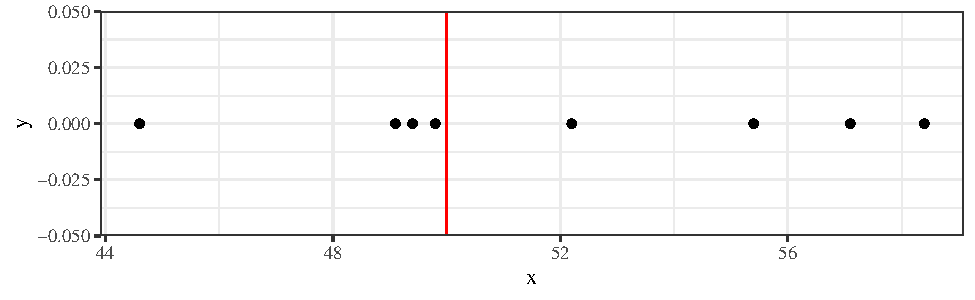
\includegraphics{R-anvisningar_files/figure-latex/unnamed-chunk-95-1} \end{center}

I grafen ser vi att värdena ligger jämt spridda kring 50, så 50 är nog ganska rimligt som medelvärde, men låt oss göra ett formellt test.
I R kan ett t-test genomföras med \texttt{t.test()}.

\begin{Shaded}
\begin{Highlighting}[]
\FunctionTok{t.test}\NormalTok{(dat}\SpecialCharTok{$}\NormalTok{x, }\AttributeTok{mu =} \DecValTok{50}\NormalTok{)   }\CommentTok{\# Ett t{-}test på variabeln x i dataobjektet dat}
\end{Highlighting}
\end{Shaded}

\begin{verbatim}
## 
##  One Sample t-test
## 
## data:  dat$x
## t = 1.2086, df = 7, p-value = 0.266
## alternative hypothesis: true mean is not equal to 50
## 95 percent confidence interval:
##  48.08713 55.91287
## sample estimates:
## mean of x 
##        52
\end{verbatim}

Utskriften ger ett p-värde från vilket vi kan dra en slutsats. I det här fallet är p-värdet högt (över fem procent) så vi kan inte förkasta nollhypotesen (vilken är att populationsmedelvärdet är lika med 50).

Vi tittar nu på stegen bakom t-testet.
Ett t-test bygger, som alla hypotestest, på en serie steg:

\begin{enumerate}
\def\labelenumi{\arabic{enumi}.}
\tightlist
\item
  sätt upp en \emph{nollhypotes} och en \emph{alternativhypotes},
\item
  beräkna ett \emph{testvärde} från en testfunktion,
\item
  identifiera en \emph{testfördelning},
\item
  beräkna ett \emph{p-värde}, eller uppskatta ett genom att ställa testvärde mot ett kritiskt värde,
\item
  dra en klar \emph{slutsats} om statistisk signifikans.
\end{enumerate}

Vi vill testa om medelskörden är skild från 50, så hypoteser ges av

\begin{itemize}
\tightlist
\item
  H0: mu lika med 50
\item
  H1: mu ej lika med 50
\end{itemize}

Alternativhypotesen är tvåsidig - vi tittar både på möjligheten att populationsmedelvärdet är större och på möjligheten att det är mindre.

\begin{exercise}[Ensidig mothypotes]
Hur hade hypoteserna sett ut om vi ville testa om medelvärdet är \emph{större} än 50?
\end{exercise}

Vårt mål är att testa ett medelvärde och det är rimligt att anta normalfördelning för den undersökta variabeln. Det lämpliga testet är då ett t-test för ett stickprov och testvärdet kan beräknas av en testfunktion som ges av det observerade stickprovet minus nollhypotesens värde, delat på standardavvikelsen delat på roten ur antalet observationer. Låt oss beräkna detta i flera steg och jämföra med utskriften från \texttt{t.test()}.

\begin{Shaded}
\begin{Highlighting}[]
\FunctionTok{mean}\NormalTok{(dat}\SpecialCharTok{$}\NormalTok{x)}
\end{Highlighting}
\end{Shaded}

\begin{verbatim}
## [1] 52
\end{verbatim}

\begin{Shaded}
\begin{Highlighting}[]
\FunctionTok{sd}\NormalTok{(dat}\SpecialCharTok{$}\NormalTok{x)}
\end{Highlighting}
\end{Shaded}

\begin{verbatim}
## [1] 4.680354
\end{verbatim}

\begin{Shaded}
\begin{Highlighting}[]
\NormalTok{t\_value }\OtherTok{\textless{}{-}}\NormalTok{ (}\DecValTok{52} \SpecialCharTok{{-}} \DecValTok{50}\NormalTok{) }\SpecialCharTok{/}\NormalTok{ (}\FloatTok{4.680354} \SpecialCharTok{/} \FunctionTok{sqrt}\NormalTok{(}\DecValTok{8}\NormalTok{))}
\end{Highlighting}
\end{Shaded}

\begin{exercise}[Operationsordning]
Räkna ut samma sak på miniräknare eller telefon. Vad händer om man missar parenteser runt \texttt{4.680354\ /\ sqrt(8)}?
\end{exercise}

\begin{exercise}[t-värdets delar]
Vad händer med t-värdet om något av följande händer, givet att övriga delar är desamma? Det observerade medelvärdet (här 52) ökar. Nollhypotesens värde (här 50) minskar. Standardavvikelsen (här 4.680354) minskar. Antalet observationer (här 8) ökar.

Testa genom att ändra värdena i kodstycket ovan och beräkna \texttt{t\_value} på nytt.
\end{exercise}

Nästa steg är att identifiera testfördelning, det vill säga den slumpfördelning testvärdet följet om nollhypotesen är sann. Fördelningen ges i regel av statistisk teori. I det här fallet är testfördelning en t-fördelning med n - 1 frihetsgrader. Vi har åtta observationer, så antalet frihetsgrader blir 7. I R kan man ta fram täthetsfunktionen för en t-fördelning med \texttt{dt()} och fördelningsfunktionen med \texttt{pt()}.

\begin{Shaded}
\begin{Highlighting}[]
\NormalTok{dat\_t }\OtherTok{\textless{}{-}} \FunctionTok{data.frame}\NormalTok{(}\AttributeTok{x =} \FunctionTok{seq}\NormalTok{(}\SpecialCharTok{{-}}\DecValTok{4}\NormalTok{, }\DecValTok{4}\NormalTok{, }\FloatTok{0.1}\NormalTok{)) }\SpecialCharTok{\%\textgreater{}\%} 
  \FunctionTok{mutate}\NormalTok{(}\AttributeTok{p =} \FunctionTok{dt}\NormalTok{(x, }\AttributeTok{df =} \DecValTok{7}\NormalTok{),}
         \AttributeTok{P =} \FunctionTok{pt}\NormalTok{(x, }\AttributeTok{df =} \DecValTok{7}\NormalTok{))}

\FunctionTok{ggplot}\NormalTok{(dat\_t, }\FunctionTok{aes}\NormalTok{(x, p)) }\SpecialCharTok{+}
  \FunctionTok{geom\_line}\NormalTok{()}
\end{Highlighting}
\end{Shaded}

\begin{center}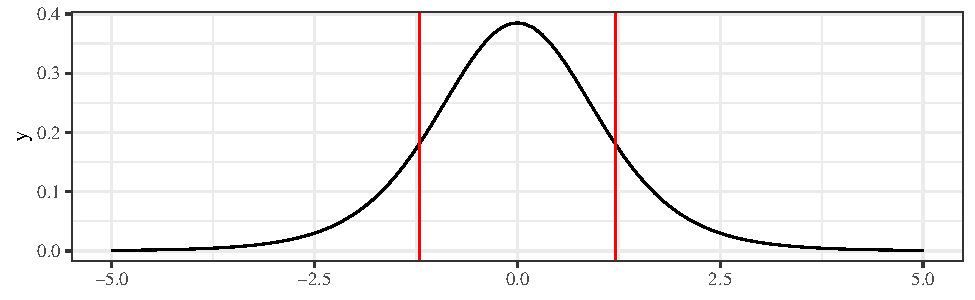
\includegraphics{R-anvisningar_files/figure-latex/unnamed-chunk-98-1} \end{center}

\begin{Shaded}
\begin{Highlighting}[]
\FunctionTok{ggplot}\NormalTok{(dat\_t, }\FunctionTok{aes}\NormalTok{(x, P)) }\SpecialCharTok{+}
  \FunctionTok{geom\_line}\NormalTok{()}
\end{Highlighting}
\end{Shaded}

\begin{center}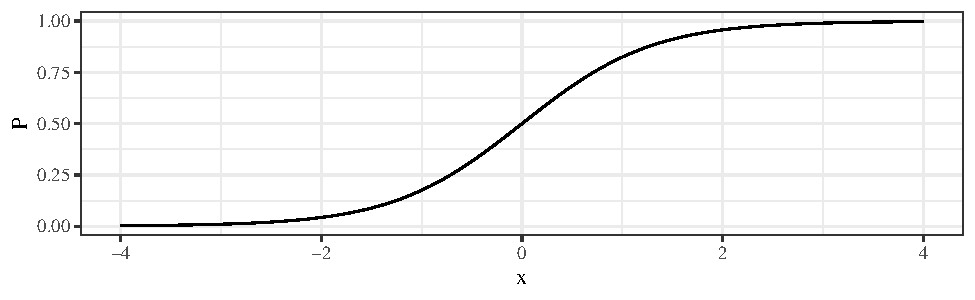
\includegraphics{R-anvisningar_files/figure-latex/unnamed-chunk-98-2} \end{center}

Nästa steg i ett hypotestest är att ta fram ett p-värdet. P-värdet kan illustreras som ytan under t-fördelning \emph{bortom} test-värdet. I ett tvåsidigt test tar vi med bägge svansarna.

\begin{Shaded}
\begin{Highlighting}[]
\FunctionTok{ggplot}\NormalTok{(dat\_t) }\SpecialCharTok{+}
  \FunctionTok{geom\_line}\NormalTok{(}\FunctionTok{aes}\NormalTok{(x, p)) }\SpecialCharTok{+}
  \FunctionTok{geom\_ribbon}\NormalTok{(}\FunctionTok{aes}\NormalTok{(}\AttributeTok{x =}\NormalTok{ x, }\AttributeTok{ymin =} \DecValTok{0}\NormalTok{, }\AttributeTok{ymax =}\NormalTok{ p), }\AttributeTok{data =}\NormalTok{ dat\_t }\SpecialCharTok{\%\textgreater{}\%} \FunctionTok{filter}\NormalTok{(x }\SpecialCharTok{\textgreater{}} \FunctionTok{abs}\NormalTok{(t\_value)), }\AttributeTok{fill =} \StringTok{"salmon"}\NormalTok{) }\SpecialCharTok{+}
  \FunctionTok{geom\_ribbon}\NormalTok{(}\FunctionTok{aes}\NormalTok{(}\AttributeTok{x =}\NormalTok{ x, }\AttributeTok{ymin =} \DecValTok{0}\NormalTok{, }\AttributeTok{ymax =}\NormalTok{ p), }\AttributeTok{data =}\NormalTok{ dat\_t }\SpecialCharTok{\%\textgreater{}\%} \FunctionTok{filter}\NormalTok{(x }\SpecialCharTok{\textless{}} \SpecialCharTok{{-}}\FunctionTok{abs}\NormalTok{(t\_value)), }\AttributeTok{fill =} \StringTok{"salmon"}\NormalTok{)}
\end{Highlighting}
\end{Shaded}

\begin{center}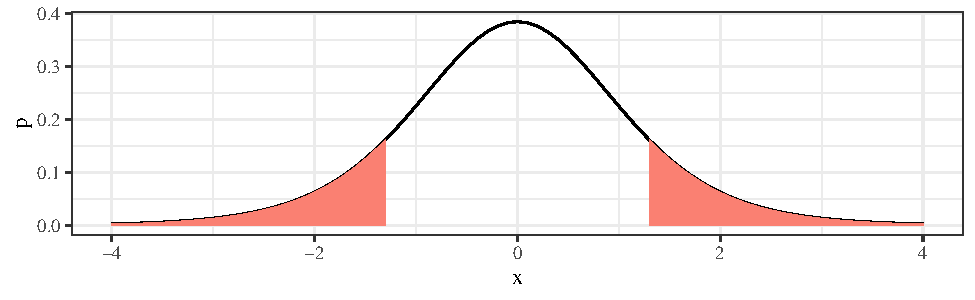
\includegraphics{R-anvisningar_files/figure-latex/unnamed-chunk-99-1} \end{center}

De röda ytorna i \emph{svansarna} motsvarar p-värdet. De anger sannolikheten att få ett större t-värde än det vi fått, under antagandet att nollhypotesen stämmer. Vi kan beräkna p-värdet med \texttt{pt()}. För ett tvåsidigt test multipliceras värdet med 2.

\begin{Shaded}
\begin{Highlighting}[]
\DecValTok{2} \SpecialCharTok{*} \FunctionTok{pt}\NormalTok{(}\SpecialCharTok{{-}}\FunctionTok{abs}\NormalTok{(t\_value), }\DecValTok{7}\NormalTok{) }\CommentTok{\# Tvåsidigt p{-}värde}
\end{Highlighting}
\end{Shaded}

\begin{verbatim}
## [1] 0.2660402
\end{verbatim}

P-värdet ges av 0.266. En tolkning av det är om försöket upprepas ett stort antal gånger och nollhypotesen är sann, kommer vi 26.6 procent av gångerna få ett större testvärde än 1.2086. Det vi observerar är ganska sannolikt under nollhypotesen, vilket tyder på att nollhypotesen är rimligt.

Det avslutande steget är att dra en formell slutsats och ge ett tydligt svar. Det klassiska sättet är att jämföra p-värdet med en förbestämd signifikansnivå, oftast fem procent. Här är p-värdet över den nivån, så vi kan inte förkasta nollhyptesen. Slutsatsen är att det \emph{inte} finns någon signifikant skillnad från 50 i havreskörd.

\begin{exercise}[Kritiskt värde]

Om man gör ett t-test för hand kan man inte enkelt ta fram ett p-värde, men kan se om p-värdet är större eller mindre än fem procent genom att ställa testvärdet mot ett kritiskt värde. Använd en tabell för t-fördelning för att hitta det kritiska värdet.

I R kan man ta fram kritiska värden med \texttt{qt()}. För fem procent i svansarna har man 0.025 i respektive svans och det kritiska värdet ges av

\begin{Shaded}
\begin{Highlighting}[]
\FunctionTok{qt}\NormalTok{(}\FloatTok{0.975}\NormalTok{, }\DecValTok{7}\NormalTok{)}
\end{Highlighting}
\end{Shaded}

\begin{verbatim}
## [1] 2.364624
\end{verbatim}

\end{exercise}

Som visades i början har R en specifik funktion för t-testet, \texttt{t.test()}. Funktionens argument är datan man testar och ett nollhypotesvärde \texttt{mu}. Om man vill ha ett ensidigt test kan det sättas med argumentet \texttt{alternative}. För vår data ges testet av

\begin{Shaded}
\begin{Highlighting}[]
\FunctionTok{t.test}\NormalTok{(dat}\SpecialCharTok{$}\NormalTok{x, }\AttributeTok{mu =} \DecValTok{50}\NormalTok{) }\CommentTok{\# Tvåsidigt test}
\end{Highlighting}
\end{Shaded}

\begin{verbatim}
## 
##  One Sample t-test
## 
## data:  dat$x
## t = 1.2086, df = 7, p-value = 0.266
## alternative hypothesis: true mean is not equal to 50
## 95 percent confidence interval:
##  48.08713 55.91287
## sample estimates:
## mean of x 
##        52
\end{verbatim}

Funktionen skriver ut det beräkna t-värdet, antal frihetsgrader och p-värdet.

\begin{exercise}[Ensigt test]
Använd \texttt{?t.test} för att ta fram funktionens hjälpsida. Försök att utifrån hjälpsidan beräkna ett \emph{ensidigt} test för att se om medelskörden är \emph{större} än 50.
\end{exercise}

\begin{exercise}[Ny nollhypotes]
Upprepa det tvåsidiga testet från exemplet ovan. Testa denna gång om medelskörden är skild från 48. Dra en tydlig slutsats.
\end{exercise}

\begin{exercise}[Importera smältpunkt-data]

På canvassidan finns en excelfil med data för kursens uppgifter \emph{Uppgiftsdata.xlsx}. Fliken \emph{Smältdata} innehåller data för en legerings smältpunkt.

Ladda ner filen till lämplig plats på datorn och importera datan genom att fylla i följande rad.

\begin{Shaded}
\begin{Highlighting}[]
\FunctionTok{library}\NormalTok{(readxl)}
\NormalTok{dat\_smält }\OtherTok{\textless{}{-}} \FunctionTok{read\_excel}\NormalTok{(}\StringTok{"\_\_\_"}\NormalTok{, }\AttributeTok{sheet =} \StringTok{"Smältpunkt"}\NormalTok{)}
\end{Highlighting}
\end{Shaded}

\end{exercise}

\begin{exercise}[Plotta smältpunkt-data]
Illustrera smältpunktsdatan på samma sätt som exempeldatan genom att fylla i följande kod. Vårt mål är att testa om medelvärde är skilt från 1050, vilket här kan noteras med ett vertikalt streck vid 1050.

\begin{Shaded}
\begin{Highlighting}[]
\FunctionTok{ggplot}\NormalTok{(\_\_\_, }\FunctionTok{aes}\NormalTok{(}\AttributeTok{x =}\NormalTok{ Smältpunkt, }\AttributeTok{y =} \DecValTok{0}\NormalTok{)) }\SpecialCharTok{+} 
  \FunctionTok{\_\_\_}\NormalTok{() }\SpecialCharTok{+}
  \FunctionTok{geom\_vline}\NormalTok{(}\AttributeTok{xintercept =}\NormalTok{ \_\_\_, }\AttributeTok{color =} \StringTok{"red"}\NormalTok{)}
\end{Highlighting}
\end{Shaded}

Kan man utifrån grafen säga om 1050 är ett rimligt medelvärde för populationen, givet det stickprov vi observerar?
\end{exercise}

\begin{exercise}[Hypotestest för hand]

Genomför ett t-test för hand för att se om medelsmältpunkten är skild från 1050. Skriv ut tydliga hypoteser. Medelvärde och standardavvikelse ges av följande.

\begin{Shaded}
\begin{Highlighting}[]
\FunctionTok{mean}\NormalTok{(dat\_smält}\SpecialCharTok{$}\NormalTok{Smältpunkt)}
\FunctionTok{sd}\NormalTok{(dat\_smält}\SpecialCharTok{$}\NormalTok{Smältpunkt)}
\end{Highlighting}
\end{Shaded}

Ett kritiskt värde kan tas från en tabell över t-fördelningen eller beräknas i R med

\begin{Shaded}
\begin{Highlighting}[]
\FunctionTok{qt}\NormalTok{(}\FloatTok{0.975}\NormalTok{, }\AttributeTok{df =} \DecValTok{9}\NormalTok{)}
\end{Highlighting}
\end{Shaded}

\end{exercise}

\begin{exercise}[Hypotestest i R]
Genomför ett t-test med funktionen \texttt{t.test()} för att se om medelsmältpunkten är skild från 1050.
\end{exercise}

\section{Konfidensintervall för normalfördelad data}\label{konfidensintervall-fuxf6r-normalfuxf6rdelad-data}

För exemplet på havredata tittade vi på två olika värden för nollhypotesen.

\begin{Shaded}
\begin{Highlighting}[]
\FunctionTok{t.test}\NormalTok{(dat}\SpecialCharTok{$}\NormalTok{x, }\AttributeTok{mu =} \DecValTok{50}\NormalTok{)}
\FunctionTok{t.test}\NormalTok{(dat}\SpecialCharTok{$}\NormalTok{x, }\AttributeTok{mu =} \DecValTok{48}\NormalTok{)}
\end{Highlighting}
\end{Shaded}

Från p-värdena kan man dra slutsatsen att förkasta vid nollhypotesen att mu är 48, men inte förkasta vid nollhypotesen att mu är 50. Värdet 50 är alltså i någon mening ett mer troligt värde på populationens medelvärde än vad 48 är. \emph{Konfidensintervall} kan ses som en generalisering av den tanken: ett konfidensintervall ger ett spann av värden där man \emph{inte} förkastar. Intervallet tolkas vanligen som att det täcker det sanna populationsmedelvärdet med en viss konfidens.

För ett stickprov och antagen normalfördelning ges konfidensintervallet av

medelvärde ± kvantil från t-fördelningen x standardavvikelse delat på roten ur antalet observationer

Kvantilen från t-fördelningen kan hämtas från en tabell (samma som det kritiska värdet i testet) eller genom R. Antalet frihetsgrader ges av antalet observationer minus ett. I det här fallet ges delarna av

\begin{Shaded}
\begin{Highlighting}[]
\FunctionTok{mean}\NormalTok{(dat}\SpecialCharTok{$}\NormalTok{x)}
\end{Highlighting}
\end{Shaded}

\begin{verbatim}
## [1] 52
\end{verbatim}

\begin{Shaded}
\begin{Highlighting}[]
\FunctionTok{sd}\NormalTok{(dat}\SpecialCharTok{$}\NormalTok{x)}
\end{Highlighting}
\end{Shaded}

\begin{verbatim}
## [1] 4.680354
\end{verbatim}

\begin{Shaded}
\begin{Highlighting}[]
\FunctionTok{qt}\NormalTok{(}\FloatTok{0.975}\NormalTok{, }\DecValTok{7}\NormalTok{)}
\end{Highlighting}
\end{Shaded}

\begin{verbatim}
## [1] 2.364624
\end{verbatim}

och konfidensintervallet ges alltså av

52 ± 2.365 * 4.680 / sqrt(8)

\begin{exercise}[Konfidensintervall för hand]
Ta fram medelvärde, standardavvikelse och kritiskt värde för smältpunktsdata, med hjälp av R (eller en tabell för det kritiska värdet). Beräkna konfidensintervallet för smältpunktsdatan för hand.
\end{exercise}

Funktionen \texttt{t.test()} ger automatiskt ett konfidensintervall, direkt under utfallet av testet. Notera att konfidensintervallet inte beror på nollhypotesen. Konfidensintervall kan beräknas med skilda konfidensnivåer, oftast 95 procent, vilket sätts med argumentet \texttt{conf.level}.

\begin{exercise}[Konfidensnivå]
Gör lämplig ändring i koden nedan för att beräkna ett 99-procentigt konfidensintervall, istället för ett 95-procentigt.

\begin{Shaded}
\begin{Highlighting}[]
\FunctionTok{t.test}\NormalTok{(dat}\SpecialCharTok{$}\NormalTok{x, }\AttributeTok{conf.level =} \FloatTok{0.95}\NormalTok{)}
\end{Highlighting}
\end{Shaded}

\begin{verbatim}
## 
##  One Sample t-test
## 
## data:  dat$x
## t = 31.425, df = 7, p-value = 8.538e-09
## alternative hypothesis: true mean is not equal to 0
## 95 percent confidence interval:
##  48.08713 55.91287
## sample estimates:
## mean of x 
##        52
\end{verbatim}

Är ett 99-procentigt konfidensintervall bredare eller smalare än ett 95-procentigt?
\end{exercise}

\begin{exercise}[Ensidiga konfidensintervall]
I en tidigare uppgift användes argumentet \texttt{alternative} för att göra ett ensidigt test med \texttt{t.test()}. Vad händer med konfidensintervallet om man anger ett ensidigt test?
\end{exercise}

\begin{exercise}[Konfidensintervall för smältdata]
Ta datan över smältpunkter och beräkna ett konfidensintervall med \texttt{t.test()}. Tolka intervallet.
\end{exercise}

Ett konfidensintervall illustreras ofta med en felstapel. Vi kan lägga till en till den punktgraf vi tidigare sett för observationerna.

\begin{Shaded}
\begin{Highlighting}[]
\NormalTok{interval }\OtherTok{\textless{}{-}} \FunctionTok{t.test}\NormalTok{(dat}\SpecialCharTok{$}\NormalTok{x)}\SpecialCharTok{$}\NormalTok{conf.int}
\FunctionTok{ggplot}\NormalTok{(dat, }\FunctionTok{aes}\NormalTok{(x, }\DecValTok{0}\NormalTok{)) }\SpecialCharTok{+}
  \FunctionTok{geom\_point}\NormalTok{() }\SpecialCharTok{+}
  \FunctionTok{annotate}\NormalTok{(}\StringTok{"errorbar"}\NormalTok{, }\AttributeTok{xmin =}\NormalTok{ interval[}\DecValTok{1}\NormalTok{], }\AttributeTok{xmax =}\NormalTok{ interval[}\DecValTok{2}\NormalTok{], }\AttributeTok{y =} \SpecialCharTok{{-}}\DecValTok{1}\NormalTok{, }\AttributeTok{width =} \FloatTok{0.1}\NormalTok{)}
\end{Highlighting}
\end{Shaded}

\begin{center}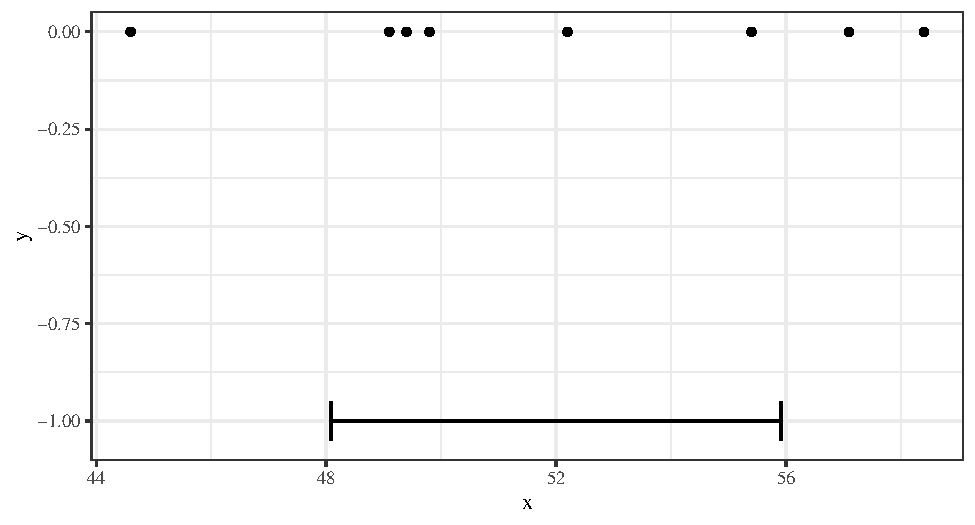
\includegraphics{R-anvisningar_files/figure-latex/unnamed-chunk-110-1} \end{center}

\begin{exercise}[Illustration av smältdata]
Använd exempelillustrationen för havredata till en liknande illustration av smältpunktsdatan.
\end{exercise}

\section{Normalfördelad data och centrala gränsvärdesatsen}\label{normalfuxf6rdelad-data-och-centrala-gruxe4nsvuxe4rdesatsen}

Eftersom t-testet bygger på att data är normalfördelad är det förstås bra att kunna undersöka om det antagandet stämmer. Ett sätt är att göra ett histogram över datan - om den underliggande variabeln är normalfördelad bör stickprovet ge den typiska klockformen. Det här kräver dock ganska mycket data. Ta ett histogram för havredatan som exempel

\begin{Shaded}
\begin{Highlighting}[]
\FunctionTok{ggplot}\NormalTok{(dat, }\FunctionTok{aes}\NormalTok{(x)) }\SpecialCharTok{+} \FunctionTok{geom\_histogram}\NormalTok{(}\AttributeTok{bins =} \DecValTok{5}\NormalTok{)}
\end{Highlighting}
\end{Shaded}

\begin{center}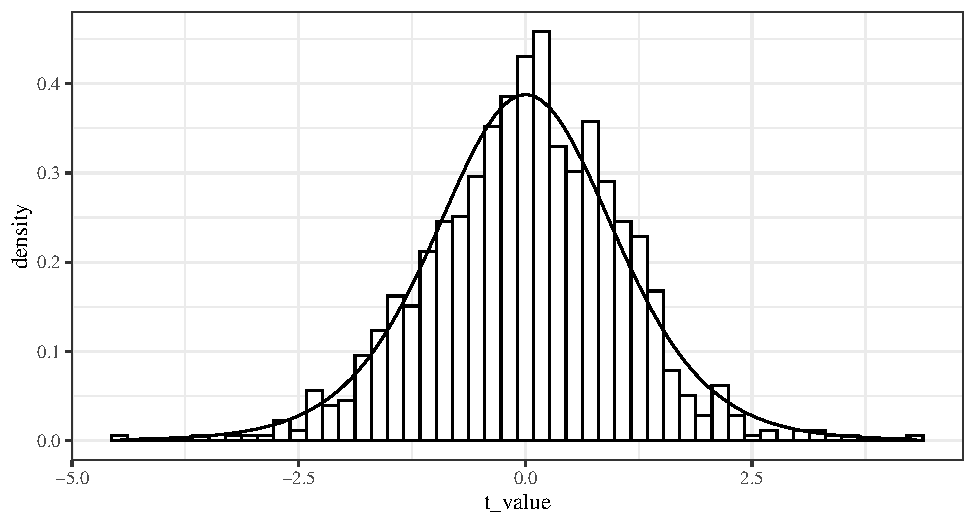
\includegraphics{R-anvisningar_files/figure-latex/unnamed-chunk-111-1} \end{center}

Uppenbarligen helt meningslöst. Låt oss titta på histogram över genererad normalfördelad data.

\begin{Shaded}
\begin{Highlighting}[]
\NormalTok{n }\OtherTok{\textless{}{-}} \DecValTok{10}
\FunctionTok{ggplot}\NormalTok{() }\SpecialCharTok{+} \FunctionTok{geom\_histogram}\NormalTok{(}\FunctionTok{aes}\NormalTok{(}\AttributeTok{x =} \FunctionTok{rnorm}\NormalTok{(n)), }\AttributeTok{bins =} \DecValTok{30}\NormalTok{)}
\end{Highlighting}
\end{Shaded}

\begin{center}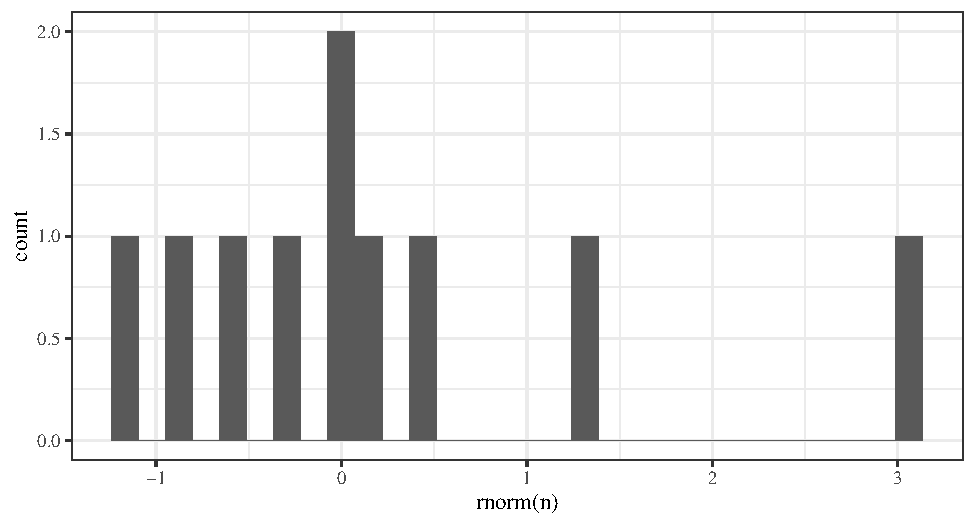
\includegraphics{R-anvisningar_files/figure-latex/unnamed-chunk-112-1} \end{center}

\begin{exercise}[Histogram för normalfördelning]
Testa koden ovan för lite olika värden på \texttt{n}. Det kan vara nyttigt att sätta antalet staplar \texttt{bins} för att få ett bättre histogram. Hur stort måste n vara för att ge en karaktäristisk klockform för histogrammet?
\end{exercise}

Ett annat vanligt alternativ för att grafisk undersöka om data följer en ungefärlig normalfördelning är en QQ-graf (\emph{QQ-plot}). En qq-graf är ett spridningsdiagram med teoretiska kvantiler på en axel och datans kvantiler på den andra axeln. Om data perfekt följer en normalfördelning kommer grafen visa en rak diagonal linje. En QQ-graf kan tas fram med \texttt{qqnorm()} eller \texttt{geom\_qq()} i en ggplot. En diagonal linje för jämförelse kan läggas till med \texttt{geom\_qq\_line()}.

\begin{Shaded}
\begin{Highlighting}[]
\FunctionTok{ggplot}\NormalTok{(dat, }\FunctionTok{aes}\NormalTok{(}\AttributeTok{sample =}\NormalTok{ x)) }\SpecialCharTok{+} \FunctionTok{geom\_qq}\NormalTok{() }\SpecialCharTok{+} \FunctionTok{geom\_qq\_line}\NormalTok{()}
\end{Highlighting}
\end{Shaded}

\begin{center}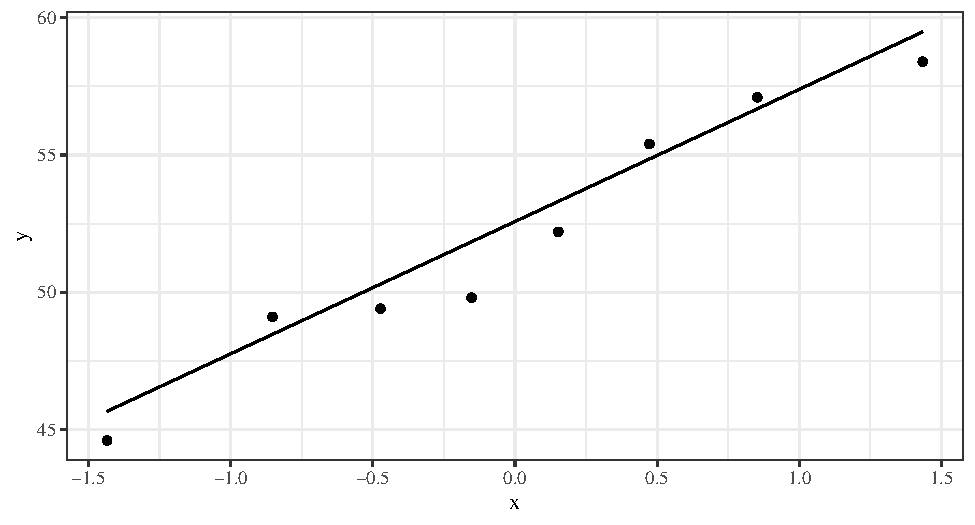
\includegraphics{R-anvisningar_files/figure-latex/unnamed-chunk-113-1} \end{center}

Punkterna ligger nära linjen. Vi kan återigen demonstrera med lite genererad data.

\begin{Shaded}
\begin{Highlighting}[]
\NormalTok{n }\OtherTok{\textless{}{-}} \DecValTok{10}
\NormalTok{dat\_norm }\OtherTok{\textless{}{-}} \FunctionTok{data.frame}\NormalTok{(}\AttributeTok{x =} \FunctionTok{rnorm}\NormalTok{(n))}
\FunctionTok{ggplot}\NormalTok{(dat\_norm, }\FunctionTok{aes}\NormalTok{(}\AttributeTok{sample =}\NormalTok{ x)) }\SpecialCharTok{+} \FunctionTok{geom\_qq}\NormalTok{() }\SpecialCharTok{+} \FunctionTok{geom\_qq\_line}\NormalTok{()}
\end{Highlighting}
\end{Shaded}

\begin{center}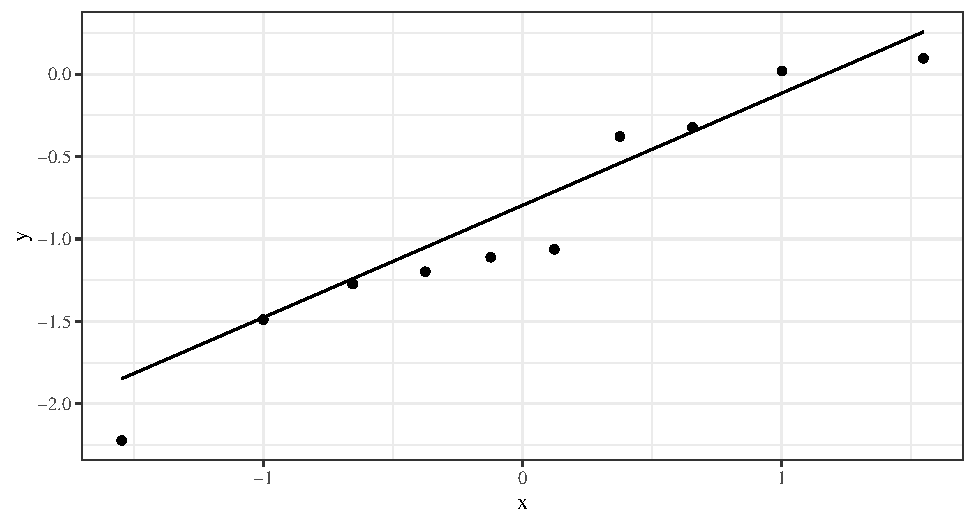
\includegraphics{R-anvisningar_files/figure-latex/unnamed-chunk-114-1} \end{center}

\begin{exercise}[Histogram för normalfördelning]
Funktionen \texttt{runif()} ger slumpmässiga värden mellan 0 och 1. Testa att ändra i kodstycket ovan så att slumptal genereras med \texttt{runif()} istället för \texttt{rnorm()}. Hur påverkar det QQ-grafen?
\end{exercise}

\section{Centrala gränsvärdesatsen}\label{centrala-gruxe4nsvuxe4rdesatsen}

Även om data inte är normalfördelad kan t-testet vara ett lämpligt val av test. Detta beror på \emph{centrala gränsvärdesatsen}, som säger att summor (och därmed även medelvärden) av lika slumpvariabler går mot en normalfördelning där antalet observationer ökar. Den tidigare uppgiften gav att \texttt{runif()} inte ger normalfördelad data. Vad händer om vi tar medelvärdet av flera observationer från \texttt{runif()}? Följande kod beräknar tiotusen medelvärden av två observationer.

\begin{Shaded}
\begin{Highlighting}[]
\NormalTok{n }\OtherTok{\textless{}{-}} \DecValTok{2}

\NormalTok{dat\_sim\_unif }\OtherTok{\textless{}{-}} \FunctionTok{expand\_grid}\NormalTok{(}\AttributeTok{Observation =} \DecValTok{1}\SpecialCharTok{:}\NormalTok{n, }\AttributeTok{Upprepning =} \DecValTok{1}\SpecialCharTok{:}\DecValTok{10000}\NormalTok{) }\SpecialCharTok{\%\textgreater{}\%} 
  \FunctionTok{mutate}\NormalTok{(}\AttributeTok{x =} \FunctionTok{runif}\NormalTok{(}\FunctionTok{n}\NormalTok{())) }\SpecialCharTok{\%\textgreater{}\%} 
  \FunctionTok{group\_by}\NormalTok{(Upprepning) }\SpecialCharTok{\%\textgreater{}\%} 
  \FunctionTok{summarise}\NormalTok{(}\AttributeTok{x =} \FunctionTok{mean}\NormalTok{(x))}

\FunctionTok{ggplot}\NormalTok{(dat\_sim\_unif, }\FunctionTok{aes}\NormalTok{(x)) }\SpecialCharTok{+} \FunctionTok{geom\_histogram}\NormalTok{(}\AttributeTok{bins =} \DecValTok{50}\NormalTok{)}
\end{Highlighting}
\end{Shaded}

\begin{center}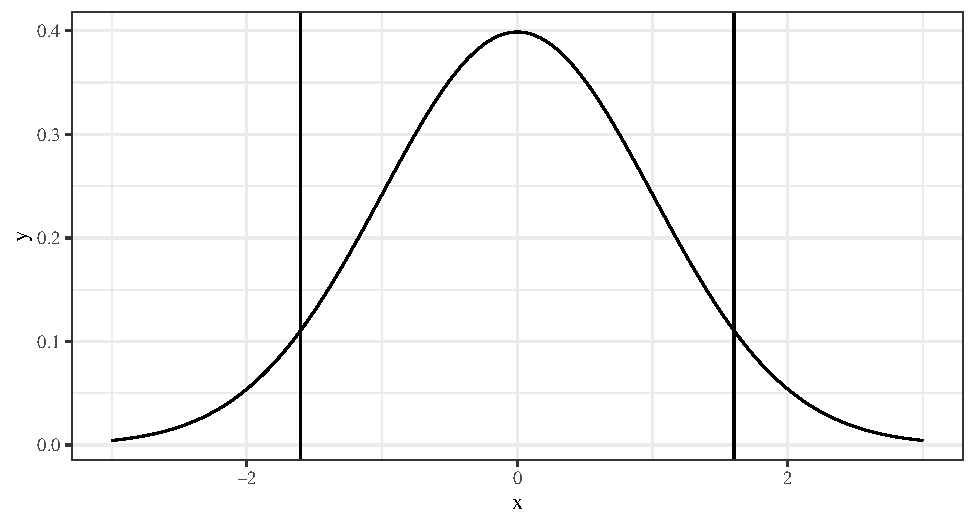
\includegraphics{R-anvisningar_files/figure-latex/unnamed-chunk-115-1} \end{center}

\begin{Shaded}
\begin{Highlighting}[]
\FunctionTok{ggplot}\NormalTok{(dat\_sim\_unif, }\FunctionTok{aes}\NormalTok{(}\AttributeTok{sample =}\NormalTok{ x)) }\SpecialCharTok{+} \FunctionTok{geom\_qq}\NormalTok{() }\SpecialCharTok{+} \FunctionTok{geom\_qq\_line}\NormalTok{()}
\end{Highlighting}
\end{Shaded}

\begin{center}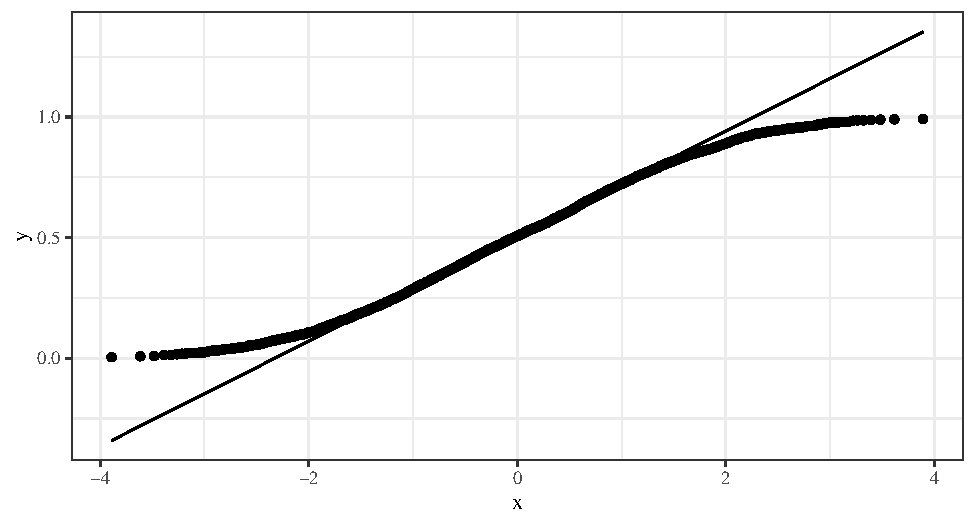
\includegraphics{R-anvisningar_files/figure-latex/unnamed-chunk-115-2} \end{center}

Fördelningen för summan är inte likformig, men inte heller särskilt normalfördelad. Vad händer om vi ökar antal termer i summan?

\begin{exercise}[Antalet observationer för normalfördelning]
Vad måste ändras i koden ovan för beräkna medelvärdet av tio observationer? Följer de medelvärdena en ungefärlig normalfördelning? Vad är det lägsta antalet observationer som ger ungefärligen normalfördelade medelvärden?
\end{exercise}

Under en tidigare datorövning såg vi exempel på diskreta fördelningar: binomial- och poissonfördelningarna. Vi ska senare titta på specifika test för variabler som följer en diskret fördelning, men centrala gränsvärdesatsen kan även då rättfärdiga ett t-test. Ta som exempel medelvärdet av tio observationer som följer en poissonfördelning med lambda = 10.

\begin{Shaded}
\begin{Highlighting}[]
\NormalTok{n }\OtherTok{\textless{}{-}} \DecValTok{10}
\NormalTok{lambda }\OtherTok{\textless{}{-}} \DecValTok{10}
\NormalTok{dat\_sim\_unif }\OtherTok{\textless{}{-}} \FunctionTok{expand\_grid}\NormalTok{(}\AttributeTok{Observation =} \DecValTok{1}\SpecialCharTok{:}\NormalTok{n, }\AttributeTok{Upprepning =} \DecValTok{1}\SpecialCharTok{:}\DecValTok{10000}\NormalTok{) }\SpecialCharTok{\%\textgreater{}\%} 
  \FunctionTok{mutate}\NormalTok{(}\AttributeTok{x =} \FunctionTok{rpois}\NormalTok{(}\FunctionTok{n}\NormalTok{(), }\AttributeTok{lambda =}\NormalTok{ lambda)) }\SpecialCharTok{\%\textgreater{}\%} 
  \FunctionTok{group\_by}\NormalTok{(Upprepning) }\SpecialCharTok{\%\textgreater{}\%} 
  \FunctionTok{summarise}\NormalTok{(}\AttributeTok{x =} \FunctionTok{mean}\NormalTok{(x))}

\FunctionTok{ggplot}\NormalTok{(dat\_sim\_unif, }\FunctionTok{aes}\NormalTok{(x)) }\SpecialCharTok{+} \FunctionTok{geom\_histogram}\NormalTok{(}\AttributeTok{bins =} \DecValTok{30}\NormalTok{)}
\end{Highlighting}
\end{Shaded}

\begin{center}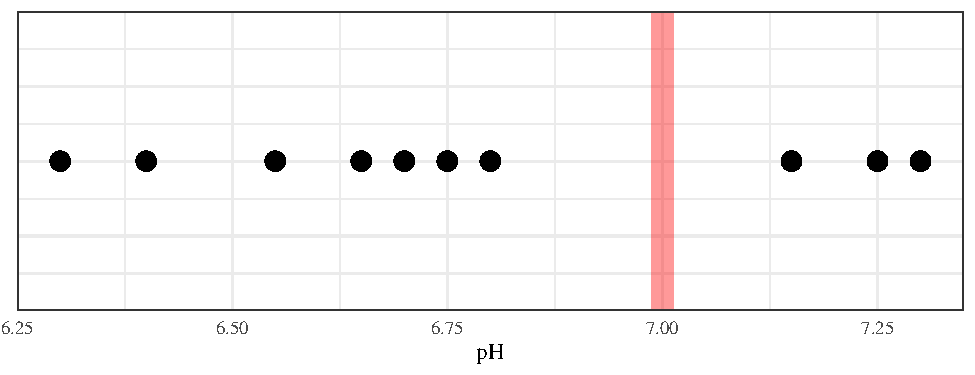
\includegraphics{R-anvisningar_files/figure-latex/unnamed-chunk-116-1} \end{center}

\begin{Shaded}
\begin{Highlighting}[]
\FunctionTok{ggplot}\NormalTok{(dat\_sim\_unif, }\FunctionTok{aes}\NormalTok{(}\AttributeTok{sample =}\NormalTok{ x)) }\SpecialCharTok{+} \FunctionTok{geom\_qq}\NormalTok{() }\SpecialCharTok{+} \FunctionTok{geom\_qq\_line}\NormalTok{()}
\end{Highlighting}
\end{Shaded}

\begin{center}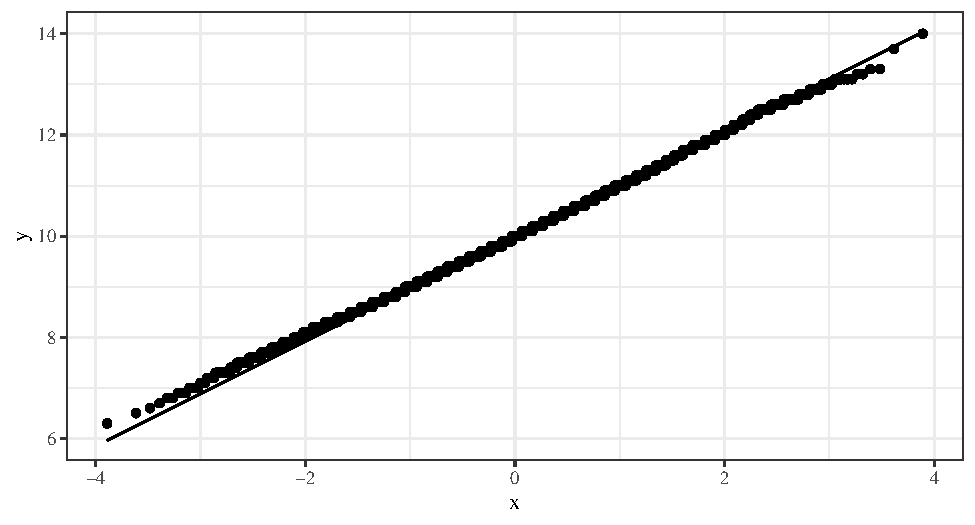
\includegraphics{R-anvisningar_files/figure-latex/unnamed-chunk-116-2} \end{center}

Histogrammet visar på en typisk klockform och punkterna följer linjen \emph{ungefärligt}. QQ-grafens trappeffekt är typisk för diskret data. Det här tyder alltså på att t-testet är ett acceptabelt alternativ om man har en poissonfördelning med lambda runt tio och gör tio upprepningar.

\begin{exercise}[Svag normalapproximation]
Testa att minska värdena på n och lambda. Vad är de lägsta värdena som ger ett histogram med en symmetrisk fördelning och punkter nära linjen i QQ-grafen?
\end{exercise}

Det kan också finnas situationer där någon matematisk transformation kan göra icke-normal data till normalfördelad data. Vanliga transformationer är att ta en kvadratrot eller att \emph{logaritmera} datan. Som exempel kan vi återvända till Gapminder-datan vi använde i en tidigare datorövning. Paketet \texttt{patchwork} kan användas för att placera flera grafer bredvid varandra. Den exakta koden är mindre viktig här.

\begin{Shaded}
\begin{Highlighting}[]
\FunctionTok{library}\NormalTok{(gapminder)}
\NormalTok{gapminder\_2007 }\OtherTok{\textless{}{-}}\NormalTok{ gapminder }\SpecialCharTok{\%\textgreater{}\%} \FunctionTok{filter}\NormalTok{(year }\SpecialCharTok{==} \DecValTok{2007}\NormalTok{)}

\NormalTok{g1 }\OtherTok{\textless{}{-}} \FunctionTok{ggplot}\NormalTok{(gapminder\_2007, }\FunctionTok{aes}\NormalTok{(pop)) }\SpecialCharTok{+} \FunctionTok{geom\_histogram}\NormalTok{(}\AttributeTok{bins =} \DecValTok{30}\NormalTok{)}
\NormalTok{g2 }\OtherTok{\textless{}{-}} \FunctionTok{ggplot}\NormalTok{(gapminder\_2007, }\FunctionTok{aes}\NormalTok{(}\AttributeTok{sample =}\NormalTok{ pop)) }\SpecialCharTok{+} \FunctionTok{geom\_qq}\NormalTok{() }\SpecialCharTok{+} \FunctionTok{geom\_qq\_line}\NormalTok{()}
\NormalTok{g3 }\OtherTok{\textless{}{-}} \FunctionTok{ggplot}\NormalTok{(gapminder\_2007, }\FunctionTok{aes}\NormalTok{(}\FunctionTok{sqrt}\NormalTok{(pop))) }\SpecialCharTok{+} \FunctionTok{geom\_histogram}\NormalTok{(}\AttributeTok{bins =} \DecValTok{30}\NormalTok{)}
\NormalTok{g4 }\OtherTok{\textless{}{-}} \FunctionTok{ggplot}\NormalTok{(gapminder\_2007, }\FunctionTok{aes}\NormalTok{(}\AttributeTok{sample =} \FunctionTok{sqrt}\NormalTok{(pop))) }\SpecialCharTok{+} \FunctionTok{geom\_qq}\NormalTok{() }\SpecialCharTok{+} \FunctionTok{geom\_qq\_line}\NormalTok{()}
\NormalTok{g5 }\OtherTok{\textless{}{-}} \FunctionTok{ggplot}\NormalTok{(gapminder\_2007, }\FunctionTok{aes}\NormalTok{(}\FunctionTok{log10}\NormalTok{(pop))) }\SpecialCharTok{+} \FunctionTok{geom\_histogram}\NormalTok{(}\AttributeTok{bins =} \DecValTok{30}\NormalTok{)}
\NormalTok{g6 }\OtherTok{\textless{}{-}} \FunctionTok{ggplot}\NormalTok{(gapminder\_2007, }\FunctionTok{aes}\NormalTok{(}\AttributeTok{sample =} \FunctionTok{log10}\NormalTok{(pop))) }\SpecialCharTok{+} \FunctionTok{geom\_qq}\NormalTok{() }\SpecialCharTok{+} \FunctionTok{geom\_qq\_line}\NormalTok{()}

\FunctionTok{library}\NormalTok{(patchwork)}
\NormalTok{g1 }\SpecialCharTok{+}\NormalTok{ g3 }\SpecialCharTok{+}\NormalTok{ g5 }\SpecialCharTok{+}\NormalTok{ g2 }\SpecialCharTok{+}\NormalTok{ g4 }\SpecialCharTok{+}\NormalTok{ g6}
\end{Highlighting}
\end{Shaded}

\begin{center}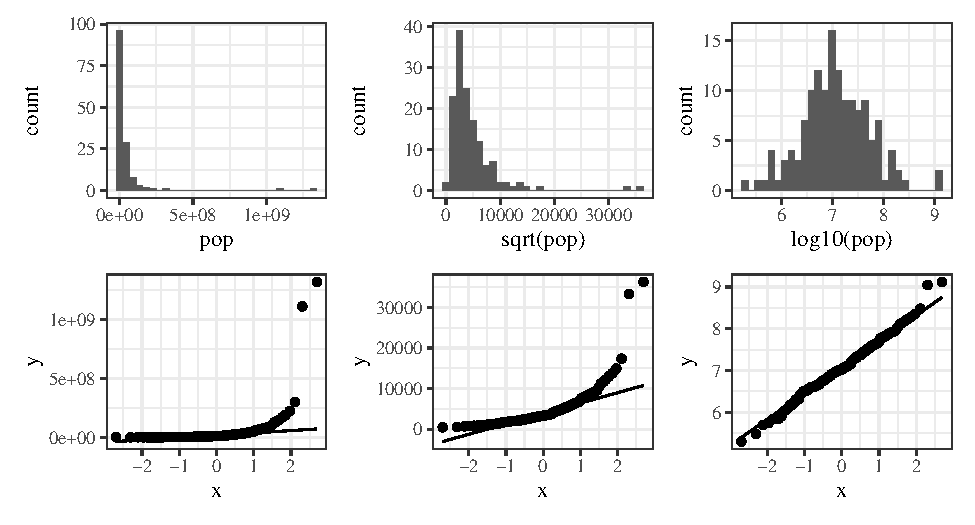
\includegraphics{R-anvisningar_files/figure-latex/unnamed-chunk-117-1} \end{center}

I grafen har vi den ursprungliga variabeln (befolkning per land 2007), den kvadratrot-transformerade variabeln (\texttt{sqrt()}) och den log-transformerade variabeln (\texttt{log10()}). De två första fallen påverkas kraftigt av extremvärden och är klart icke-normala medan den log-transformerade variabeln ger en ungefärlig normalkurva och följer diagonalen väl i QQ-grafen.

\begin{exercise}[Transformera medellivslängd]
Använd kodstycket ovan som mall och ta fram grafer för medellivslängd (\texttt{lifeExp}) istället för befolkningsstorlek (\texttt{pop}). Visar grafen samma mönster som för befolkningsdatan?
\end{exercise}

\section{Bonus. Simuleringar för t-test och konfidensintervall}\label{bonus.-simuleringar-fuxf6r-t-test-och-konfidensintervall}

Följande kod simulerar ett dataset om tio observationer från en normalfördelning med medelvärde 7 och standardavvikelse 5, beräknar ett hypotestest med nollhypotesen att populationsmedelvärdet är 7, och beräknar ett konfidensintervall.

\begin{Shaded}
\begin{Highlighting}[]
\NormalTok{dat\_sim }\OtherTok{\textless{}{-}} \FunctionTok{data.frame}\NormalTok{(}\AttributeTok{x =} \FunctionTok{rnorm}\NormalTok{(}\DecValTok{10}\NormalTok{, }\AttributeTok{mean =} \DecValTok{7}\NormalTok{, }\AttributeTok{sd =} \DecValTok{5}\NormalTok{))}
\FunctionTok{t.test}\NormalTok{(dat\_sim}\SpecialCharTok{$}\NormalTok{x, }\AttributeTok{mu =} \DecValTok{7}\NormalTok{)}
\end{Highlighting}
\end{Shaded}

\begin{verbatim}
## 
##  One Sample t-test
## 
## data:  dat_sim$x
## t = -1.9103, df = 9, p-value = 0.08842
## alternative hypothesis: true mean is not equal to 7
## 95 percent confidence interval:
##  0.8958046 7.5147998
## sample estimates:
## mean of x 
##  4.205302
\end{verbatim}

\begin{exercise}[Upprepad simulering]
Kör de två raderna i stycket ovan ett tiotal gånger. Du bör se att man ibland förkastar nollhypotesen trots att den ska stämma. Kan du få en känsla för hur stor andel av gångerna man felaktigt förkastar?
\end{exercise}

Låt oss upprepa simuleringen tusen gånger. Ett sätt är att upprepa ett steg flera gånger är genom en for-loop.

\begin{Shaded}
\begin{Highlighting}[]
\NormalTok{dat\_sim }\OtherTok{\textless{}{-}} \FunctionTok{data.frame}\NormalTok{()}
\ControlFlowTok{for}\NormalTok{(i }\ControlFlowTok{in} \DecValTok{1}\SpecialCharTok{:}\DecValTok{1000}\NormalTok{)\{}
\NormalTok{  new\_data }\OtherTok{\textless{}{-}} \FunctionTok{data.frame}\NormalTok{(}\AttributeTok{x =} \FunctionTok{rnorm}\NormalTok{(}\DecValTok{10}\NormalTok{, }\AttributeTok{mean =} \DecValTok{7}\NormalTok{, }\AttributeTok{sd =} \DecValTok{5}\NormalTok{))}
\NormalTok{  test }\OtherTok{\textless{}{-}} \FunctionTok{t.test}\NormalTok{(new\_data}\SpecialCharTok{$}\NormalTok{x, }\AttributeTok{mu =} \DecValTok{7}\NormalTok{)}
\NormalTok{  new\_results }\OtherTok{\textless{}{-}} \FunctionTok{data.frame}\NormalTok{(}\AttributeTok{t\_value =}\NormalTok{ test}\SpecialCharTok{$}\NormalTok{statistic, }\AttributeTok{p\_value =}\NormalTok{ test}\SpecialCharTok{$}\NormalTok{p.value,}
               \AttributeTok{ci\_lower =}\NormalTok{ test}\SpecialCharTok{$}\NormalTok{conf.int[}\DecValTok{1}\NormalTok{], }\AttributeTok{ci\_upper =}\NormalTok{ test}\SpecialCharTok{$}\NormalTok{conf.int[}\DecValTok{2}\NormalTok{])}
\NormalTok{  dat\_sim }\OtherTok{\textless{}{-}} \FunctionTok{bind\_rows}\NormalTok{(dat\_sim, new\_results)}
\NormalTok{\}}
\end{Highlighting}
\end{Shaded}

Enligt statistisk teori ska t-värdet följa en t-fördelning med nio frihetsgrader. Vi kan undersöka det genom ett histogram med en överliggande t-fördelning.

\begin{Shaded}
\begin{Highlighting}[]
\FunctionTok{ggplot}\NormalTok{(dat\_sim) }\SpecialCharTok{+}
  \FunctionTok{geom\_histogram}\NormalTok{(}\FunctionTok{aes}\NormalTok{(t\_value, }\AttributeTok{y =}\NormalTok{ ..density..), }\AttributeTok{bins =} \DecValTok{50}\NormalTok{, }\AttributeTok{fill =} \StringTok{"white"}\NormalTok{, }\AttributeTok{color =} \StringTok{"black"}\NormalTok{) }\SpecialCharTok{+}
  \FunctionTok{geom\_function}\NormalTok{(}\AttributeTok{fun =}\NormalTok{ dt, }\AttributeTok{args =} \FunctionTok{list}\NormalTok{(}\AttributeTok{df =} \DecValTok{9}\NormalTok{), }\AttributeTok{color =} \StringTok{"red"}\NormalTok{, }\AttributeTok{size =} \DecValTok{1}\NormalTok{)}
\end{Highlighting}
\end{Shaded}

\begin{center}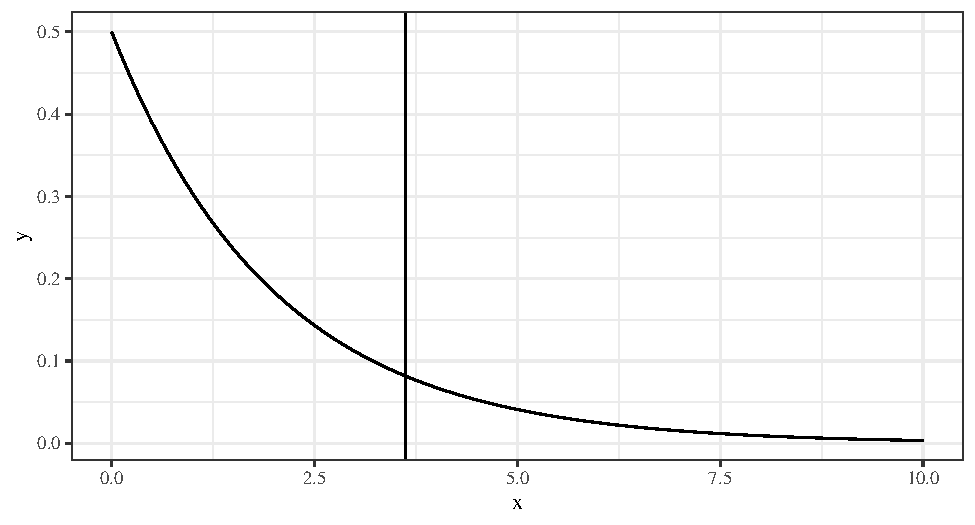
\includegraphics{R-anvisningar_files/figure-latex/unnamed-chunk-120-1} \end{center}

Den teoretiska t-fördelning passar histogrammet nästan perfekt.

Vidare ska p-värdet vara under fem procent fem procent av gångerna.

\begin{Shaded}
\begin{Highlighting}[]
\FunctionTok{mean}\NormalTok{(dat\_sim}\SpecialCharTok{$}\NormalTok{p\_value }\SpecialCharTok{\textless{}} \FloatTok{0.05}\NormalTok{)}
\end{Highlighting}
\end{Shaded}

\begin{verbatim}
## [1] 0.05
\end{verbatim}

Även det stämmer någorlunda väl. Det här innebär alltså att om man har en signifikansnivå på fem procent kommer man förkasta nollhypotesen fem procent av gångerna även om nollhypotesen stämmer. Det kallas ett \emph{falskt positivt} utfall.

\begin{exercise}[Simulerade konfidensintervall]
Hur många av de simulerade konfidensintervallen täcker värdet 7?
\end{exercise}

\begin{exercise}[Signifikant skillnad]
Stycket nedan simulerar data när populationsmedelvärdet är 9 och t-test har nollhypotesen att populationsmedelvärdet är 7. Här vill vi alltså förkasta nollhypotesen.

\begin{Shaded}
\begin{Highlighting}[]
\NormalTok{dat\_sim }\OtherTok{\textless{}{-}} \FunctionTok{data.frame}\NormalTok{()}
\ControlFlowTok{for}\NormalTok{(i }\ControlFlowTok{in} \DecValTok{1}\SpecialCharTok{:}\DecValTok{1000}\NormalTok{)\{}
\NormalTok{  new\_data }\OtherTok{\textless{}{-}} \FunctionTok{data.frame}\NormalTok{(}\AttributeTok{x =} \FunctionTok{rnorm}\NormalTok{(}\DecValTok{10}\NormalTok{, }\AttributeTok{mean =} \DecValTok{9}\NormalTok{, }\AttributeTok{sd =} \DecValTok{5}\NormalTok{))}
\NormalTok{  test }\OtherTok{\textless{}{-}} \FunctionTok{t.test}\NormalTok{(new\_data}\SpecialCharTok{$}\NormalTok{x, }\AttributeTok{mu =} \DecValTok{7}\NormalTok{)}
\NormalTok{  new\_results }\OtherTok{\textless{}{-}} \FunctionTok{data.frame}\NormalTok{(}\AttributeTok{t\_value =}\NormalTok{ test}\SpecialCharTok{$}\NormalTok{statistic, }\AttributeTok{p\_value =}\NormalTok{ test}\SpecialCharTok{$}\NormalTok{p.value,}
               \AttributeTok{ci\_lower =}\NormalTok{ test}\SpecialCharTok{$}\NormalTok{conf.int[}\DecValTok{1}\NormalTok{], }\AttributeTok{ci\_upper =}\NormalTok{ test}\SpecialCharTok{$}\NormalTok{conf.int[}\DecValTok{2}\NormalTok{])}
\NormalTok{  dat\_sim }\OtherTok{\textless{}{-}} \FunctionTok{bind\_rows}\NormalTok{(dat\_sim, new\_results)}
\NormalTok{\}}
\end{Highlighting}
\end{Shaded}

Använd kod från den första simuleringen för att undersöka hur väl histogrammet stämmer med den teoretiska fördelningen och för att se hur stor andel av gångerna man förkastar nollhypotesen på signifikansnivån 5 procent.
\end{exercise}

\begin{exercise}[50/50]
Stycket nedan simulerar data när populationsmedelvärdet är 9 och t-test har nollhypotesen att populationsmedelvärdet är 7. Ändra värdet för n och se hur det påverkar andelen gånger man förkastar nollhypotesen.

\begin{Shaded}
\begin{Highlighting}[]
\NormalTok{n }\OtherTok{\textless{}{-}} \DecValTok{10}

\NormalTok{dat\_sim }\OtherTok{\textless{}{-}} \FunctionTok{data.frame}\NormalTok{()}
\ControlFlowTok{for}\NormalTok{(i }\ControlFlowTok{in} \DecValTok{1}\SpecialCharTok{:}\DecValTok{1000}\NormalTok{)\{}
\NormalTok{  new\_data }\OtherTok{\textless{}{-}} \FunctionTok{data.frame}\NormalTok{(}\AttributeTok{x =} \FunctionTok{rnorm}\NormalTok{(n, }\AttributeTok{mean =} \DecValTok{9}\NormalTok{, }\AttributeTok{sd =} \DecValTok{5}\NormalTok{))}
\NormalTok{  test }\OtherTok{\textless{}{-}} \FunctionTok{t.test}\NormalTok{(new\_data}\SpecialCharTok{$}\NormalTok{x, }\AttributeTok{mu =} \DecValTok{7}\NormalTok{)}
\NormalTok{  new\_results }\OtherTok{\textless{}{-}} \FunctionTok{data.frame}\NormalTok{(}\AttributeTok{t\_value =}\NormalTok{ test}\SpecialCharTok{$}\NormalTok{statistic, }\AttributeTok{p\_value =}\NormalTok{ test}\SpecialCharTok{$}\NormalTok{p.value,}
               \AttributeTok{ci\_lower =}\NormalTok{ test}\SpecialCharTok{$}\NormalTok{conf.int[}\DecValTok{1}\NormalTok{], }\AttributeTok{ci\_upper =}\NormalTok{ test}\SpecialCharTok{$}\NormalTok{conf.int[}\DecValTok{2}\NormalTok{])}
\NormalTok{  dat\_sim }\OtherTok{\textless{}{-}} \FunctionTok{bind\_rows}\NormalTok{(dat\_sim, new\_results)}
\NormalTok{\}}

\FunctionTok{mean}\NormalTok{(dat\_sim}\SpecialCharTok{$}\NormalTok{p\_value }\SpecialCharTok{\textless{}} \FloatTok{0.05}\NormalTok{)}
\end{Highlighting}
\end{Shaded}

Ungefär hur många observationer behövs för att ha femtio procents sannolikhet att förkasta nollhypotesen?
\end{exercise}

\begin{exercise}[Konfidensintervallets bredd]
Ett konfidensintervall blir smalare och smalare ju större stickprovet är. Koden nedan ger medelvärdet för stickprovsbredden i simulerad data med standardavvikelsen 1.

\begin{Shaded}
\begin{Highlighting}[]
\NormalTok{n }\OtherTok{\textless{}{-}} \DecValTok{10}

\NormalTok{dat\_sim }\OtherTok{\textless{}{-}} \FunctionTok{data.frame}\NormalTok{()}
\ControlFlowTok{for}\NormalTok{(i }\ControlFlowTok{in} \DecValTok{1}\SpecialCharTok{:}\DecValTok{1000}\NormalTok{)\{}
\NormalTok{  new\_data }\OtherTok{\textless{}{-}} \FunctionTok{data.frame}\NormalTok{(}\AttributeTok{x =} \FunctionTok{rnorm}\NormalTok{(n, }\AttributeTok{mean =} \DecValTok{0}\NormalTok{, }\AttributeTok{sd =} \DecValTok{1}\NormalTok{))}
\NormalTok{  test }\OtherTok{\textless{}{-}} \FunctionTok{t.test}\NormalTok{(new\_data}\SpecialCharTok{$}\NormalTok{x, }\AttributeTok{mu =} \DecValTok{7}\NormalTok{)}
\NormalTok{  new\_results }\OtherTok{\textless{}{-}} \FunctionTok{data.frame}\NormalTok{(}\AttributeTok{t\_value =}\NormalTok{ test}\SpecialCharTok{$}\NormalTok{statistic, }\AttributeTok{p\_value =}\NormalTok{ test}\SpecialCharTok{$}\NormalTok{p.value,}
               \AttributeTok{ci\_lower =}\NormalTok{ test}\SpecialCharTok{$}\NormalTok{conf.int[}\DecValTok{1}\NormalTok{], }\AttributeTok{ci\_upper =}\NormalTok{ test}\SpecialCharTok{$}\NormalTok{conf.int[}\DecValTok{2}\NormalTok{])}
\NormalTok{  dat\_sim }\OtherTok{\textless{}{-}} \FunctionTok{bind\_rows}\NormalTok{(dat\_sim, new\_results)}
\NormalTok{\}}

\FunctionTok{mean}\NormalTok{(dat\_sim}\SpecialCharTok{$}\NormalTok{ci\_upper }\SpecialCharTok{{-}}\NormalTok{ dat\_sim}\SpecialCharTok{$}\NormalTok{ci\_lower)}
\end{Highlighting}
\end{Shaded}

Ungefär hur många observationer behövs för att konfidensintervallets bredd ska bli under 1, under 0.9, under 0.8, och så vidare ned till 0.1?
\end{exercise}

\chapter{Ett stickprov av icke-normalfördelad data}\label{ett-stickprov-av-icke-normalfuxf6rdelad-data}

Datorövning 4 handlar om hypotestest och konfidensintervall för ett stickprov av icke-normalfördelad data. Efter övningen ska vi kunna

\begin{itemize}
\item
  genomföra och tolka ett z-test för proportioner,
\item
  genomföra och tolka ett chi-två-test för nominal data
\item
  beräkna och tolka ett konfidensintervall för proportioner,
\item
  använda simulerad data för att förstå testens egenskaper.
\end{itemize}

Om det finns tid för en bonussektion kommer vi också titta på interaktiva kartor med \texttt{leaflet}.

\section{Repetition av datorövning 3}\label{repetition-av-datoruxf6vning-3}

När man startar en ny R-session bör man ladda de paket man vet kommer behövas med \texttt{library()}. Om paket inte finns installerade måste man först köra \texttt{install.packages()}.

\begin{Shaded}
\begin{Highlighting}[]
\CommentTok{\# install.packages("tidyverse")}
\FunctionTok{library}\NormalTok{(tidyverse)}
\end{Highlighting}
\end{Shaded}

I datorövning 4 tittade vi på analys av ett stickprov av normalfördelad data. Det underliggande upplägget är att vi vill säga något om en population genom att titta på ett stickprov. Ett \emph{t-test} kan användas för att testa en given \emph{nollhypotes}. Ett konfidensintervall ringar in populationens medelvärde med en viss konfidensgrad - oftast 95 procent. Ett normalfördelningsantagande kan undersökas med histogram eller QQ-grafer.

Ta som exempel följande data på jord-pH och låt oss anta att det är relevant att testa om populationens medelvärde är 7.

\begin{Shaded}
\begin{Highlighting}[]
\NormalTok{dat\_pH }\OtherTok{\textless{}{-}} \FunctionTok{data.frame}\NormalTok{(}\AttributeTok{pH =} \FunctionTok{c}\NormalTok{(}\FloatTok{6.3}\NormalTok{, }\FloatTok{6.55}\NormalTok{, }\FloatTok{6.75}\NormalTok{, }\FloatTok{6.4}\NormalTok{, }\FloatTok{7.25}\NormalTok{, }\FloatTok{6.65}\NormalTok{, }\FloatTok{6.8}\NormalTok{, }\FloatTok{7.3}\NormalTok{, }\FloatTok{7.15}\NormalTok{, }\FloatTok{6.7}\NormalTok{))}

\FunctionTok{ggplot}\NormalTok{(dat\_pH, }\FunctionTok{aes}\NormalTok{(pH, }\DecValTok{0}\NormalTok{)) }\SpecialCharTok{+}
  \FunctionTok{geom\_point}\NormalTok{(}\AttributeTok{size =} \DecValTok{4}\NormalTok{) }\SpecialCharTok{+}
  \FunctionTok{geom\_vline}\NormalTok{(}\AttributeTok{xintercept =} \DecValTok{7}\NormalTok{, }\AttributeTok{size =} \DecValTok{5}\NormalTok{, }\AttributeTok{color =} \StringTok{"red"}\NormalTok{, }\AttributeTok{alpha =} \FloatTok{0.4}\NormalTok{) }\SpecialCharTok{+}
  \FunctionTok{theme}\NormalTok{(}\AttributeTok{axis.text.y =} \FunctionTok{element\_blank}\NormalTok{(), }
        \AttributeTok{axis.title.y =} \FunctionTok{element\_blank}\NormalTok{(), }
        \AttributeTok{axis.ticks =} \FunctionTok{element\_blank}\NormalTok{())}
\end{Highlighting}
\end{Shaded}

\begin{center}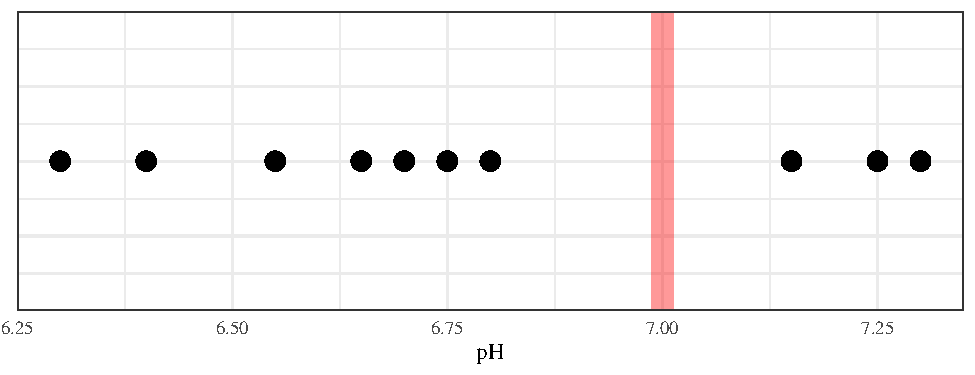
\includegraphics{R-anvisningar_files/figure-latex/unnamed-chunk-126-1} \end{center}

Hypoteser ges av

\begin{itemize}
\tightlist
\item
  H0: mu lika med 7
\item
  H1: mu ej lika med 7
\end{itemize}

Testet kan genomföras med funktionen \texttt{t.test()}.

\begin{Shaded}
\begin{Highlighting}[]
\FunctionTok{t.test}\NormalTok{(dat\_pH}\SpecialCharTok{$}\NormalTok{pH, }\AttributeTok{mu =} \DecValTok{7}\NormalTok{)}
\end{Highlighting}
\end{Shaded}

\begin{verbatim}
## 
##  One Sample t-test
## 
## data:  dat_pH$pH
## t = -1.9624, df = 9, p-value = 0.08132
## alternative hypothesis: true mean is not equal to 7
## 95 percent confidence interval:
##  6.537164 7.032836
## sample estimates:
## mean of x 
##     6.785
\end{verbatim}

Ett p-värde över 0.05 ger att vi inte förkastar nollhypotesen - den observerade skillnaden mot 7 är inte statistiskt signifikant. Konfidensintervallet ger att populationens medelvärde ligger mellan 6.54 och 7.03 med 95 procents konfidens.

En QQ-graf kan visa om det finns några avvikelser från normalantagandet. Med små datamängder är det oftast svårt att se några tydliga tecken på icke-normalitet.

\begin{Shaded}
\begin{Highlighting}[]
\FunctionTok{ggplot}\NormalTok{(dat\_pH, }\FunctionTok{aes}\NormalTok{(}\AttributeTok{sample =}\NormalTok{ pH)) }\SpecialCharTok{+}
  \FunctionTok{geom\_qq}\NormalTok{() }\SpecialCharTok{+}
  \FunctionTok{geom\_qq\_line}\NormalTok{()}
\end{Highlighting}
\end{Shaded}

\begin{center}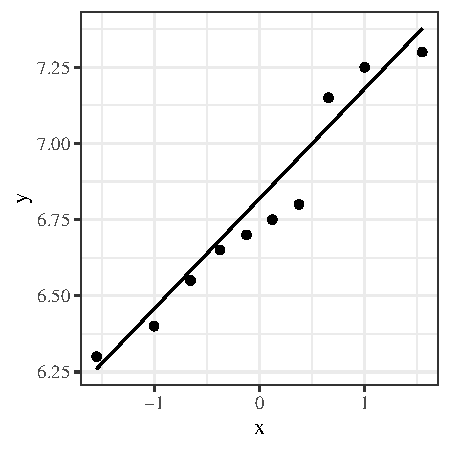
\includegraphics{R-anvisningar_files/figure-latex/unnamed-chunk-128-1} \end{center}

\section{Proportioner från binär data}\label{proportioner-fruxe5n-binuxe4r-data}

Binär data är data där en observation har ett av två utfall, vilka kan kodas som noll och ett. Man talar ibland om utfallet ett som ett \emph{positivt} utfall. Binär data kan sammanfattas med en proportion - antalet positiva utfall delat på det totala antalet upprepningar. En proportion kan testas med ett z-test för proportioner (eller \emph{relativ frekvens}). Testet följer stegen för hypotestest (Hypoteser - Testvärde - Testfördelning - P-värde (eller jämförelse med kritiskt värde) - Slutsats).

Låt oss importera lite exempeldata och beräkna ett exempel. Följande rad importerar matchresultat i fotbollsallsvenskan för damer 2000-2020.

\begin{Shaded}
\begin{Highlighting}[]
\FunctionTok{library}\NormalTok{(tidyverse)}
\NormalTok{dat\_alls }\OtherTok{\textless{}{-}} \FunctionTok{read\_csv}\NormalTok{(}\StringTok{"https://raw.githubusercontent.com/adamflr/ST0060/main/Data/Allsvenskan\%2C\%20damer\%2C\%202000{-}2020.csv"}\NormalTok{)}

\FunctionTok{ggplot}\NormalTok{(dat\_alls, }\FunctionTok{aes}\NormalTok{(hemmamal, bortamal)) }\SpecialCharTok{+}
  \FunctionTok{geom\_jitter}\NormalTok{(}\AttributeTok{size =} \FloatTok{0.1}\NormalTok{)}
\end{Highlighting}
\end{Shaded}

\begin{center}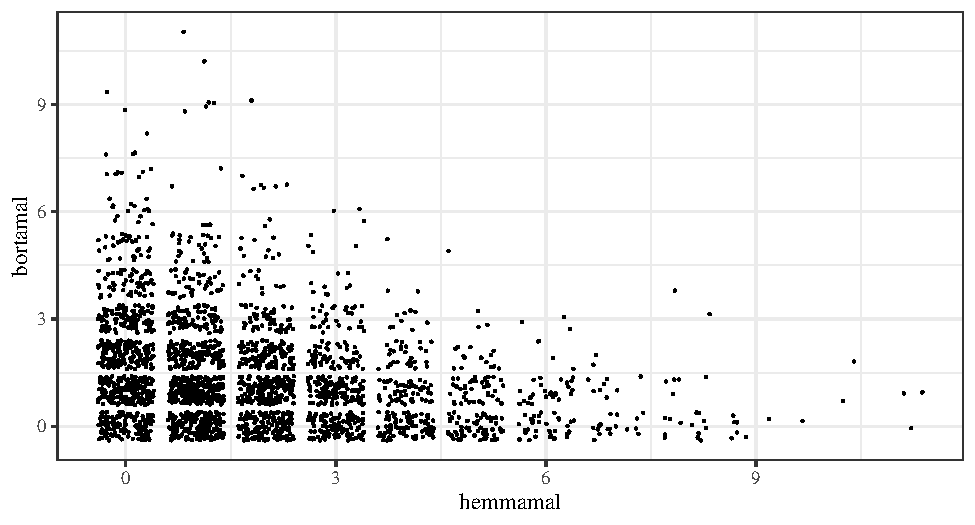
\includegraphics{R-anvisningar_files/figure-latex/unnamed-chunk-129-1} \end{center}

\begin{exercise}[En interaktiv målgraf]

Kör stycket nedan för en interaktiv målgraf. Vilken match gav det högsta antalet gjorda bortamål?

\begin{Shaded}
\begin{Highlighting}[]
\CommentTok{\# install.packages(plotly)}
\FunctionTok{library}\NormalTok{(plotly)}
\NormalTok{g }\OtherTok{\textless{}{-}} \FunctionTok{ggplot}\NormalTok{(dat\_alls, }\FunctionTok{aes}\NormalTok{(hemmamal, bortamal, }\AttributeTok{text =} \FunctionTok{paste}\NormalTok{(sasong, hemma, }\StringTok{"{-}"}\NormalTok{, borta))) }\SpecialCharTok{+}
  \FunctionTok{geom\_jitter}\NormalTok{(}\AttributeTok{size =} \FloatTok{0.1}\NormalTok{)}

\FunctionTok{ggplotly}\NormalTok{(g)}
\end{Highlighting}
\end{Shaded}

\end{exercise}

Gammal bollkunskap säger att var tredje match är en bortavinst. Vi kan testa det med ett z-test för proportioner. För att ta fram antalet bortasegrar och totalt antal matcher använder vi \texttt{count()} på kolumnen \texttt{resultat}. Man kan också använda funktionen \texttt{table()} för ett liknande resultat.

\begin{Shaded}
\begin{Highlighting}[]
\NormalTok{dat\_alls }\SpecialCharTok{\%\textgreater{}\%} \FunctionTok{count}\NormalTok{(resultat)}
\end{Highlighting}
\end{Shaded}

\begin{verbatim}
## # A tibble: 3 x 2
##   resultat       n
##   <chr>      <int>
## 1 Bortaseger   947
## 2 Hemmaseger  1285
## 3 Oavgjort     518
\end{verbatim}

\begin{Shaded}
\begin{Highlighting}[]
\FunctionTok{table}\NormalTok{(dat\_alls}\SpecialCharTok{$}\NormalTok{resultat)}
\end{Highlighting}
\end{Shaded}

\begin{verbatim}
## 
## Bortaseger Hemmaseger   Oavgjort 
##        947       1285        518
\end{verbatim}

Datan har 947 bortasegrar av totalt 947 + 1803 matcher. Vår skattade proportion \texttt{p} och totala antal \texttt{n} är alltså

\begin{Shaded}
\begin{Highlighting}[]
\NormalTok{n }\OtherTok{\textless{}{-}} \DecValTok{947} \SpecialCharTok{+} \DecValTok{1803}
\NormalTok{p\_est }\OtherTok{\textless{}{-}} \DecValTok{947} \SpecialCharTok{/}\NormalTok{ n}

\NormalTok{p\_est}
\end{Highlighting}
\end{Shaded}

\begin{verbatim}
## [1] 0.3443636
\end{verbatim}

\begin{Shaded}
\begin{Highlighting}[]
\NormalTok{n}
\end{Highlighting}
\end{Shaded}

\begin{verbatim}
## [1] 2750
\end{verbatim}

För att genomföra ett z-test sätter vi upp hypoteser om proportionen bortasegrar.

\begin{itemize}
\tightlist
\item
  Nollhypotes H0: p lika med 0.33
\item
  Alternativhypotes H1: p ej lika med 0.33
\end{itemize}

Ett test kan köras i R med \texttt{prop.test()}.

\begin{Shaded}
\begin{Highlighting}[]
\FunctionTok{prop.test}\NormalTok{(}\AttributeTok{x =} \DecValTok{947}\NormalTok{, }\AttributeTok{n =} \DecValTok{2750}\NormalTok{, }\AttributeTok{p =} \FloatTok{0.33}\NormalTok{, }\AttributeTok{correct =}\NormalTok{ F)}
\end{Highlighting}
\end{Shaded}

\begin{verbatim}
## 
##  1-sample proportions test without continuity correction
## 
## data:  947 out of 2750, null probability 0.33
## X-squared = 2.5661, df = 1, p-value = 0.1092
## alternative hypothesis: true p is not equal to 0.33
## 95 percent confidence interval:
##  0.3268327 0.3623288
## sample estimates:
##         p 
## 0.3443636
\end{verbatim}

P-värdet ställs mot en förbestämd signifikansnivå (vanligen 5 procent). I det här fallet leder det höga p-värdet till att nollhypotesen accepteras.

Om vi tar en närmre titt på testets steg brörjar vi med att beräkna ett testvärde.

\begin{Shaded}
\begin{Highlighting}[]
\NormalTok{p0 }\OtherTok{\textless{}{-}} \FloatTok{0.33}
\NormalTok{z\_value }\OtherTok{\textless{}{-}}\NormalTok{ (p\_est }\SpecialCharTok{{-}}\NormalTok{ p0) }\SpecialCharTok{/} \FunctionTok{sqrt}\NormalTok{(p0 }\SpecialCharTok{*}\NormalTok{ (}\DecValTok{1} \SpecialCharTok{{-}}\NormalTok{ p0) }\SpecialCharTok{/}\NormalTok{ n)}
\NormalTok{z\_value}
\end{Highlighting}
\end{Shaded}

\begin{verbatim}
## [1] 1.601904
\end{verbatim}

Därefter kan p-värdet räknas ut som arean under en standardiserad normalfördelning bortom z-värdet. Eftersom vi har en tvåsidig mothypotes adderas de två svansarna.

\begin{Shaded}
\begin{Highlighting}[]
\NormalTok{dat\_norm }\OtherTok{\textless{}{-}} \FunctionTok{data.frame}\NormalTok{(}\AttributeTok{x =} \FunctionTok{seq}\NormalTok{(}\SpecialCharTok{{-}}\DecValTok{4}\NormalTok{, }\DecValTok{4}\NormalTok{, }\FloatTok{0.1}\NormalTok{)) }\SpecialCharTok{\%\textgreater{}\%} 
  \FunctionTok{mutate}\NormalTok{(}\AttributeTok{p =} \FunctionTok{dnorm}\NormalTok{(x))}

\FunctionTok{ggplot}\NormalTok{(dat\_norm) }\SpecialCharTok{+}
  \FunctionTok{geom\_line}\NormalTok{(}\FunctionTok{aes}\NormalTok{(x, p)) }\SpecialCharTok{+}
  \FunctionTok{geom\_ribbon}\NormalTok{(}\FunctionTok{aes}\NormalTok{(}\AttributeTok{x =}\NormalTok{ x, }\AttributeTok{ymin =} \DecValTok{0}\NormalTok{, }\AttributeTok{ymax =}\NormalTok{ p), }\AttributeTok{data =}\NormalTok{ dat\_norm }\SpecialCharTok{\%\textgreater{}\%} \FunctionTok{filter}\NormalTok{(x }\SpecialCharTok{\textgreater{}} \FunctionTok{abs}\NormalTok{(z\_value)), }\AttributeTok{fill =} \StringTok{"salmon"}\NormalTok{) }\SpecialCharTok{+}
  \FunctionTok{geom\_ribbon}\NormalTok{(}\FunctionTok{aes}\NormalTok{(}\AttributeTok{x =}\NormalTok{ x, }\AttributeTok{ymin =} \DecValTok{0}\NormalTok{, }\AttributeTok{ymax =}\NormalTok{ p), }\AttributeTok{data =}\NormalTok{ dat\_norm }\SpecialCharTok{\%\textgreater{}\%} \FunctionTok{filter}\NormalTok{(x }\SpecialCharTok{\textless{}} \SpecialCharTok{{-}}\FunctionTok{abs}\NormalTok{(z\_value)), }\AttributeTok{fill =} \StringTok{"salmon"}\NormalTok{)}
\end{Highlighting}
\end{Shaded}

\begin{center}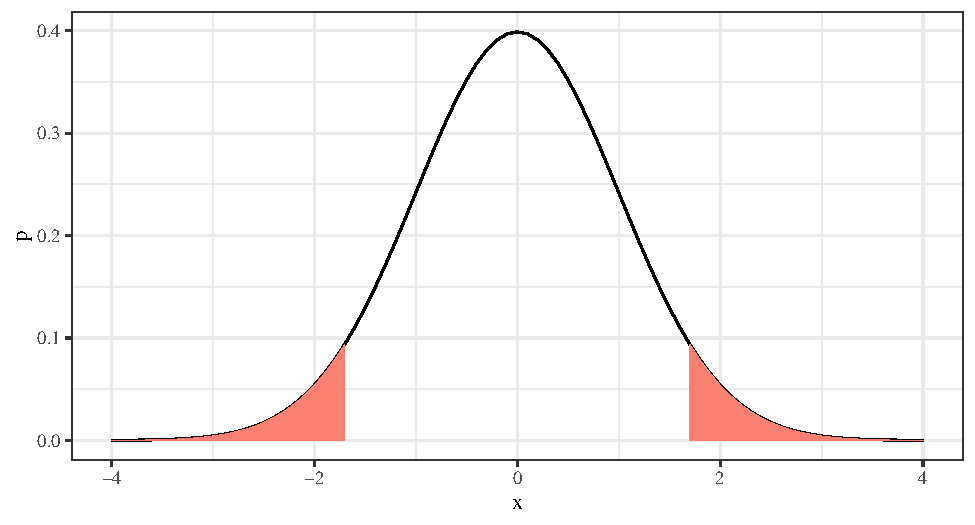
\includegraphics{R-anvisningar_files/figure-latex/unnamed-chunk-135-1} \end{center}

Areans yta kan tas fram med normalfördelningens fördelningsfunktion \texttt{pnorm()}.

\begin{Shaded}
\begin{Highlighting}[]
\DecValTok{2} \SpecialCharTok{*} \FunctionTok{pnorm}\NormalTok{(}\SpecialCharTok{{-}}\NormalTok{z\_value)}
\end{Highlighting}
\end{Shaded}

\begin{verbatim}
## [1] 0.1091769
\end{verbatim}

Testets p-värde är ungefär 11 procent. Vår observation är alltså inte ett orimligt utfall om den faktiska sannolikheten för bortaseger är 0.33 och vi kan inte förkasta nollhypotesen på femprocentsnivån.

Om man löste uppgiften för hand skulle man istället för att beräkna p-värdet jämföra z-värdet med ett kritisk värde ur en tabell. Det kritiska värdet för fem-procentig signifikans är 1.96. Vi kan också ta fram det genom \texttt{qnorm(0.975)}.

Vi kan jämföra den beräkning med den direkta R-funktionen.

\begin{Shaded}
\begin{Highlighting}[]
\FunctionTok{prop.test}\NormalTok{(}\AttributeTok{x =} \DecValTok{947}\NormalTok{, }\AttributeTok{n =} \DecValTok{2750}\NormalTok{, }\AttributeTok{p =} \FloatTok{0.33}\NormalTok{, }\AttributeTok{correct =}\NormalTok{ F)}
\end{Highlighting}
\end{Shaded}

\begin{verbatim}
## 
##  1-sample proportions test without continuity correction
## 
## data:  947 out of 2750, null probability 0.33
## X-squared = 2.5661, df = 1, p-value = 0.1092
## alternative hypothesis: true p is not equal to 0.33
## 95 percent confidence interval:
##  0.3268327 0.3623288
## sample estimates:
##         p 
## 0.3443636
\end{verbatim}

Den stegvisa beräkningen gav samma utfall som funktionen (\texttt{p-value\ =\ 0.01092}). Funktionen ger inte z-värdet utan ett chi-två-värde (2.5661). Här är det värdet lika med z-värdet i kvadrat.

\begin{Shaded}
\begin{Highlighting}[]
\NormalTok{z\_value}\SpecialCharTok{\^{}}\DecValTok{2}
\end{Highlighting}
\end{Shaded}

\begin{verbatim}
## [1] 2.566095
\end{verbatim}

\begin{exercise}[Ensidigt test]
Titta på hjälpsidan med \texttt{?prop.test}. Hur genomför man ett ensidigt test? Gör lämpligt tillägg för att testa om andelen bortasegrar är större än 0.33.
\end{exercise}

\begin{exercise}[Test för proportionen oavgjorda]

Samma gamla bollkunskap säger att 20 procent av matcher blir oavgjorda. I datan är 518 av 2750 matcher oavgjorda. Ställ upp hypoteser och fyll i koden nedan för att testa om bollkunskapen stämmer.

\begin{Shaded}
\begin{Highlighting}[]
\FunctionTok{prop.test}\NormalTok{(}\AttributeTok{x =}\NormalTok{ \_\_\_, }\AttributeTok{n =}\NormalTok{ \_\_\_, }\AttributeTok{p =}\NormalTok{ \_\_\_, }\AttributeTok{correct =}\NormalTok{ F)}
\end{Highlighting}
\end{Shaded}

\end{exercise}

\begin{exercise}[Test för proportionen hemmasegrar]

Slutligen är då resten av matcherna, 1285 av 2750, hemmasegrar. Gammal bollkunskap säger: \emph{47 procent av alla matcher är hemmasegrar}. Genomför ett z-test för att testa det påstående.

\begin{Shaded}
\begin{Highlighting}[]
\FunctionTok{prop.test}\NormalTok{(}\AttributeTok{x =}\NormalTok{ \_\_\_, }\AttributeTok{n =}\NormalTok{ \_\_\_, }\AttributeTok{p =}\NormalTok{ \_\_\_, }\AttributeTok{correct =}\NormalTok{ F)}
\end{Highlighting}
\end{Shaded}

\end{exercise}

\begin{exercise}[Population och stickprov]
Ett hypotestest bygger på en underliggande tanke med en population (med någon för oss okänd proportion positiva utfall) och ett stickprov (i vilket vi kan observera andelen positiva utfall). Det är inte alltid uppenbart vad som egentligen är populationen. I fallet med fotbollsdatan, vad kan ses som populationen? Hur långt skulle man kunna generalisera de slutsatser man kan dra från datan?
\end{exercise}

\begin{exercise}[Guldfiskgenetik]
(Fråga från Olsson, \emph{Biometri}) En teori inom genetik förutsäger att tre fjärdedelar i en grupp guldfiskar ska ha genomskinliga fjäll. Observationer ger att nittio av hundra har genomskinliga fjäll. Genomför ett test med \texttt{prop.test()} för att se om den faktiska proportionen skiljer sig från 0.75. Lös gärna först uppgiften för hand eller med miniräknare.
\end{exercise}

\begin{exercise}[Mer guldfiskgenetik]
(Fråga från Olsson, \emph{Biometri}) En konkurrerande teori inom genetik förutsäger att femton sextondelar (proportionen 0.9375) ska ha genomskinliga fjäll. Observationer ger att nittio av hundra har genomskinliga fjäll. Genomför ett test med \texttt{prop.test()} för att se om proportionen skiljer sig från 0.9375. Lös gärna först uppgiften för hand eller med miniräknare.
\end{exercise}

Hypotestestet för proportioner som används här, \emph{z-testet}, bygger på en normalapproximation av en binomialfördelning. Approximation blir bättre när antalet observationer är stort och nollhypotesens värde p0 ligger nära 0.5. En vanlig tumregel för när approximationen är giltig är att n gånger p0 gånger (1 - p0) ska vara större än 10. För fotbollsdatan över oavgjorda matcher ger det 2750 * 0.2 * 0.8 vilket är klart större än 10.

\begin{exercise}[Giltig approximation]
I det andra guldfiskexemplet är antalet observationer 100 och nollhypotesens värde 0.9375. Är normalapproximationen \emph{giltig} i det fallet?
\end{exercise}

\begin{exercise}[Fågelproportioner]
I ett naturreservat tror man fördelningen av tre fåglar (tärnmås, fiskmås och fisktärna) är 50, 30 respektive 20 procent. En studie ger antalen 115, 54 respektive 31. Genomför tre z-test för att testa den antagna andelarna. För tärnmås får man till exempel \texttt{prop.test(115,\ 200,\ p\ =\ 0.5,\ correct\ =\ F)}.
\end{exercise}

\begin{exercise}[Förbestämd signifikans]
En intressant egenskap hos proportionstest är att man redan i förväg kan beräkna vilka utfall som ger signifikanta resulat. Säg att man har möjlighet att göra 100 replikat. Ändra i stycket nedan för att hitta det högsta värde på x som ger ett \emph{icke}-signifikant utfall.

\begin{Shaded}
\begin{Highlighting}[]
\FunctionTok{prop.test}\NormalTok{(x, }\AttributeTok{n =} \DecValTok{100}\NormalTok{, }\AttributeTok{p =} \FloatTok{0.5}\NormalTok{, }\AttributeTok{correct =}\NormalTok{ F)}
\end{Highlighting}
\end{Shaded}

Det är möjligt att göra liknande beräkningar för ett t-test för normalfördelad data, men då måste man göra antaganden om standardavvikelsens storlek.
\end{exercise}

\section{Konfidensintervall för proportioner}\label{konfidensintervall-fuxf6r-proportioner}

Konstruktionen av ett konfidensintervall för en proportion är ganska lik konstruktionen för ett medelvärde. För en skattad proportion p och antal observationer n kan man beräkna p plus/minus ett z-värde från tabell gånger medelfelet, där medelfelet ges av roten ur p * (1 - p) / n.~För exemplet med bortasegrar i allsvenskan är p = 0.344 och n = 2750. Tabellvärdet hämtas från en tabell över kvantiler. För ett 95-procentigt konfidensintervall tar vi kvantilen 0.975 (2.5 procent i respektive svans) vilket ger värdet 1.96. Konfidensintervallet ges av

\begin{Shaded}
\begin{Highlighting}[]
\NormalTok{n }\OtherTok{\textless{}{-}} \DecValTok{947} \SpecialCharTok{+} \DecValTok{1803}
\NormalTok{p }\OtherTok{\textless{}{-}} \DecValTok{947} \SpecialCharTok{/}\NormalTok{ n}

\NormalTok{p }\SpecialCharTok{{-}} \FloatTok{1.96} \SpecialCharTok{*} \FunctionTok{sqrt}\NormalTok{(p }\SpecialCharTok{*}\NormalTok{ (}\DecValTok{1} \SpecialCharTok{{-}}\NormalTok{ p) }\SpecialCharTok{/}\NormalTok{ n)}
\end{Highlighting}
\end{Shaded}

\begin{verbatim}
## [1] 0.3266042
\end{verbatim}

\begin{Shaded}
\begin{Highlighting}[]
\NormalTok{p }\SpecialCharTok{+} \FloatTok{1.96} \SpecialCharTok{*} \FunctionTok{sqrt}\NormalTok{(p }\SpecialCharTok{*}\NormalTok{ (}\DecValTok{1} \SpecialCharTok{{-}}\NormalTok{ p) }\SpecialCharTok{/}\NormalTok{ n)}
\end{Highlighting}
\end{Shaded}

\begin{verbatim}
## [1] 0.3621231
\end{verbatim}

Notera att 0.33, det värde som var nollhypotesen i det tidigare testet, \emph{ingår} i intervallet. Om man tittar på utskriften från \texttt{prop.test()} kan man se ett konfidensintervall. Det intervallet är dock inte beräknat på samma sätt den formel som förekommer på föreläsningarna. För att få matchande utskrift kan vi använda paketet \texttt{binom} och funktionen \texttt{binom.asymp()}.

\begin{Shaded}
\begin{Highlighting}[]
\CommentTok{\#install.packages("binom")}
\FunctionTok{library}\NormalTok{(binom)}
\FunctionTok{binom.asymp}\NormalTok{(}\AttributeTok{x =} \DecValTok{947}\NormalTok{, }\AttributeTok{n =} \DecValTok{2750}\NormalTok{)}
\end{Highlighting}
\end{Shaded}

\begin{verbatim}
##       method   x    n      mean     lower     upper
## 1 asymptotic 947 2750 0.3443636 0.3266045 0.3621228
\end{verbatim}

\begin{exercise}[99-procentigt konfidensintervall]

Gör lämplig ändring i koden nedan för att beräkna ett 99-procentigt konfidensintervall för andelen bortasegrar.

\begin{Shaded}
\begin{Highlighting}[]
\FunctionTok{binom.asymp}\NormalTok{(}\AttributeTok{x =} \DecValTok{947}\NormalTok{, }\AttributeTok{n =} \DecValTok{2750}\NormalTok{, }\AttributeTok{conf.level =} \FloatTok{0.95}\NormalTok{)}
\end{Highlighting}
\end{Shaded}

\end{exercise}

\begin{exercise}[Perfekta utfall]
Vad händer om man försöker räkna ut ett konfidensintervall för ett perfekt utfall - t.ex. om man får 100 av 100 positiva utfall?
\end{exercise}

\begin{exercise}[Konfidensintervall för guldfiskar]
Använd funktionen \texttt{binom.asymp()} för att ta fram konfidensintervallet för andelen guldfiskar från den tidigare uppgiften. Hur förhåller sig resultatet till nollhypotesernas värden (0.75 respektive 0.9375)? Gör motsvarande beräkning med miniräknare.
\end{exercise}

\section{Chi-två-test för goodness-of-fit}\label{chi-tvuxe5-test-fuxf6r-goodness-of-fit}

Ett proportionstest kan ses som ett test av en variabel med två möjliga klasser som utfall. Ett \emph{goodness-of-fit}-test utvecklar det till valfritt antal klasser. Testet utförs som ett chi-två-test genom att beräkna ett observerat antal O och ett förväntat antal E för varje klass. Testvärdet ges av att man beräknar (O - E)\^{}2 / E för varje klass och sedan summerar. Testfunktionen är en chi-två-fördelning där antalet frihetsgrader beror på antalet klasser.

Låt oss göra ett exempel baserat på fotbollsdatan. Där hade vi utfallet 947, 518 och 1285 för bortaseger, oavgjort och hemmaseger. Klassisk bollkunskap gav oss sannolikheterna 33, 20 och 47 procent. Testets hypoteser ges av

H0: sannolikheterna för de olika utfallet ges av 33, 20 respektive 47 procent

H1: minst något utfall har en annan sannolikhet än 33, 20 respektive 47 procent

För att få de förväntade värdena E multipliceras nollhypotesens sannolikheter med det totala antalet matcher.

\begin{Shaded}
\begin{Highlighting}[]
\NormalTok{O }\OtherTok{\textless{}{-}} \FunctionTok{c}\NormalTok{(}\DecValTok{947}\NormalTok{, }\DecValTok{518}\NormalTok{, }\DecValTok{1285}\NormalTok{)}
\NormalTok{E }\OtherTok{\textless{}{-}} \FunctionTok{c}\NormalTok{(}\FloatTok{0.33}\NormalTok{,}\FloatTok{0.20}\NormalTok{,}\FloatTok{0.47}\NormalTok{) }\SpecialCharTok{*} \DecValTok{2750}
\end{Highlighting}
\end{Shaded}

\begin{exercise}[Granska E]
Skriv ut objektet \texttt{E} och jämför med de observerade värdena. Notera att de förväntade värdena inte måste vara heltal, trots att de observerade värdena förstås alltid kommer vara det.
\end{exercise}

Testvärdet beräknas genom formeln för varje term följt av summan.

\begin{Shaded}
\begin{Highlighting}[]
\NormalTok{chisq\_value }\OtherTok{\textless{}{-}} \FunctionTok{sum}\NormalTok{((O }\SpecialCharTok{{-}}\NormalTok{ E)}\SpecialCharTok{\^{}}\DecValTok{2} \SpecialCharTok{/}\NormalTok{ E)}
\end{Highlighting}
\end{Shaded}

P-värdet beräknas från en chi-två-fördelning. Antalet frihetsgrader ges av antalet klasser minus antalet skattade parametrar minus ett. I det här fallet har inga parametrar skattats från datan så antalet frihetsgrader blir två. Ett chi-två-test beräknas med kvadrater så vi är enbart intresserade av högra svansen.

\begin{Shaded}
\begin{Highlighting}[]
\NormalTok{dat\_chisq }\OtherTok{\textless{}{-}} \FunctionTok{data.frame}\NormalTok{(}\AttributeTok{x =} \FunctionTok{seq}\NormalTok{(}\DecValTok{0}\NormalTok{, }\DecValTok{10}\NormalTok{, }\FloatTok{0.1}\NormalTok{)) }\SpecialCharTok{\%\textgreater{}\%} 
  \FunctionTok{mutate}\NormalTok{(}\AttributeTok{p =} \FunctionTok{dchisq}\NormalTok{(x, }\AttributeTok{df =} \DecValTok{2}\NormalTok{))}

\FunctionTok{ggplot}\NormalTok{() }\SpecialCharTok{+}
  \FunctionTok{geom\_line}\NormalTok{(}\FunctionTok{aes}\NormalTok{(x, p), }\AttributeTok{data =}\NormalTok{ dat\_chisq) }\SpecialCharTok{+}
  \FunctionTok{geom\_ribbon}\NormalTok{(}\FunctionTok{aes}\NormalTok{(x, }\AttributeTok{ymin =} \DecValTok{0}\NormalTok{, }\AttributeTok{ymax =}\NormalTok{ p), }\AttributeTok{data =}\NormalTok{ dat\_chisq }\SpecialCharTok{\%\textgreater{}\%} \FunctionTok{filter}\NormalTok{(x }\SpecialCharTok{\textgreater{}}\NormalTok{ chisq\_value), }\AttributeTok{fill =} \StringTok{"salmon"}\NormalTok{)}
\end{Highlighting}
\end{Shaded}

\begin{center}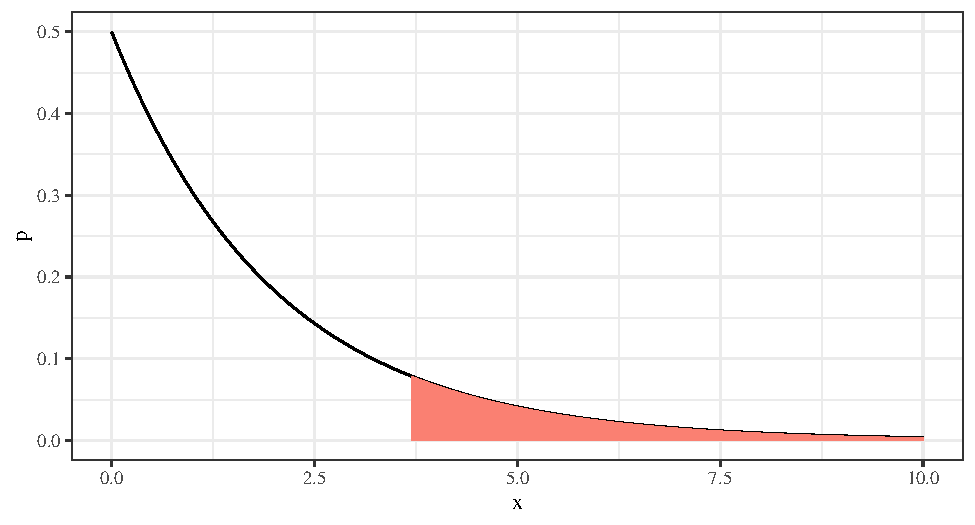
\includegraphics{R-anvisningar_files/figure-latex/unnamed-chunk-147-1} \end{center}

Man kan också beräkna ytan i svansen med \texttt{pchisq()}. Ett minus det resultatet ger den övre delen.

\begin{Shaded}
\begin{Highlighting}[]
\DecValTok{1} \SpecialCharTok{{-}} \FunctionTok{pchisq}\NormalTok{(chisq\_value, }\AttributeTok{df =} \DecValTok{2}\NormalTok{)}
\end{Highlighting}
\end{Shaded}

\begin{verbatim}
## [1] 0.1632763
\end{verbatim}

P-värdet är alltså 0.16, över den klassiska signifikansnivån på 5 procent, vilket ger att vi inte kan förkasta nollhypotesen. Om man gör ett chi-två-test för hand jämför man det observerade chi-två-värdet med ett tabellvärde över kvantiler. Tabellvärdet kan också hämtas med funktionen \texttt{qchisq()}, i det här fallet

\begin{Shaded}
\begin{Highlighting}[]
\FunctionTok{qchisq}\NormalTok{(}\FloatTok{0.95}\NormalTok{, }\AttributeTok{df =} \DecValTok{2}\NormalTok{)}
\end{Highlighting}
\end{Shaded}

\begin{verbatim}
## [1] 5.991465
\end{verbatim}

Notera att man tar 0.95 eftersom man alltid tittar på den yttre svansen i ett chi-två-test.

R har en inbyggd funktion för chi-två-test. Dess argument ges av observerade antal och sannolikheter.

\begin{Shaded}
\begin{Highlighting}[]
\FunctionTok{chisq.test}\NormalTok{(O, }\AttributeTok{p =} \FunctionTok{c}\NormalTok{(}\FloatTok{0.33}\NormalTok{, }\FloatTok{0.2}\NormalTok{, }\FloatTok{0.47}\NormalTok{))}
\end{Highlighting}
\end{Shaded}

\begin{verbatim}
## 
##  Chi-squared test for given probabilities
## 
## data:  O
## X-squared = 3.6246, df = 2, p-value = 0.1633
\end{verbatim}

Testet ger samma chi-två-värde och p-värde som beräknats ovan.

\begin{exercise}[Chi-två med två klasser]
Situationen med flera klasser kan som sagt ses som en generalisering av fallet med två klasser. Det är alltså logiskt att chi-två-test kan användas även när man har två klasser. Följande exempel ger samma test som vi sett tidigare av andelen bortasegrar.

\begin{Shaded}
\begin{Highlighting}[]
\FunctionTok{chisq.test}\NormalTok{(}\AttributeTok{x =} \FunctionTok{c}\NormalTok{(}\DecValTok{947}\NormalTok{, }\DecValTok{1803}\NormalTok{), }\AttributeTok{p =} \FunctionTok{c}\NormalTok{(}\FloatTok{0.33}\NormalTok{, }\FloatTok{0.67}\NormalTok{), }\AttributeTok{correct =}\NormalTok{ F)}
\end{Highlighting}
\end{Shaded}

\begin{verbatim}
## 
##  Chi-squared test for given probabilities
## 
## data:  c(947, 1803)
## X-squared = 2.5661, df = 1, p-value = 0.1092
\end{verbatim}

Likt \texttt{prop.test()} sätter vi \texttt{correct} till \texttt{FALSE} för att inte göra en korrektion. Notera att \texttt{x} här anges som positiva och negativa utfall istället för positiva utfall och totalt antal utfall, vilket var fallet i \texttt{prop.test()}.

Använd stycket ovan som mall för att göra uppgiften om guldfiskar som ett chi-två-test. Testa nollhypotesen att andelen positiva utfall är 0.75.
\end{exercise}

Chi-två-testet bygger på en underliggande normal-liknande approximation. En vanlig tumregel är att alla förväntade värden ska vara större än 5. R ger en varning om så inte är fallet.

\begin{Shaded}
\begin{Highlighting}[]
\FunctionTok{chisq.test}\NormalTok{(}\FunctionTok{c}\NormalTok{(}\DecValTok{6}\NormalTok{,}\DecValTok{4}\NormalTok{), }\AttributeTok{p =} \FunctionTok{c}\NormalTok{(}\FloatTok{0.51}\NormalTok{, }\FloatTok{0.49}\NormalTok{))}
\end{Highlighting}
\end{Shaded}

\begin{verbatim}
## 
##  Chi-squared test for given probabilities
## 
## data:  c(6, 4)
## X-squared = 0.32413, df = 1, p-value = 0.5691
\end{verbatim}

\begin{exercise}[Chi-två med lika sannolikheter]
En vanlig tillämpning av goodness-of-fit-testet är för att testa om alla klasser är lika sannolika. En jämn fördelning är grundinställning i \texttt{chisq.test()} så i det fallet behöver man bara ange de observerade värdena. En datainsamling om M\&M-godis gav följande antal.

\begin{Shaded}
\begin{Highlighting}[]
\NormalTok{dat\_mnm }\OtherTok{\textless{}{-}} \FunctionTok{data.frame}\NormalTok{(}\AttributeTok{Color =} \FunctionTok{c}\NormalTok{(}\StringTok{"blue"}\NormalTok{, }\StringTok{"brown"}\NormalTok{, }\StringTok{"green"}\NormalTok{, }\StringTok{"orange"}\NormalTok{, }\StringTok{"red"}\NormalTok{, }\StringTok{"yellow"}\NormalTok{),}
                      \AttributeTok{Count =} \FunctionTok{c}\NormalTok{(}\DecValTok{180}\NormalTok{, }\DecValTok{80}\NormalTok{, }\DecValTok{88}\NormalTok{, }\DecValTok{160}\NormalTok{, }\DecValTok{134}\NormalTok{, }\DecValTok{166}\NormalTok{))}

\FunctionTok{ggplot}\NormalTok{(dat\_mnm, }\FunctionTok{aes}\NormalTok{(Color, Count, }\AttributeTok{fill =}\NormalTok{ Color)) }\SpecialCharTok{+}
  \FunctionTok{geom\_col}\NormalTok{() }\SpecialCharTok{+}
  \FunctionTok{scale\_fill\_manual}\NormalTok{(}\AttributeTok{values =}\NormalTok{ dat\_mnm}\SpecialCharTok{$}\NormalTok{Color)}
\end{Highlighting}
\end{Shaded}

\begin{center}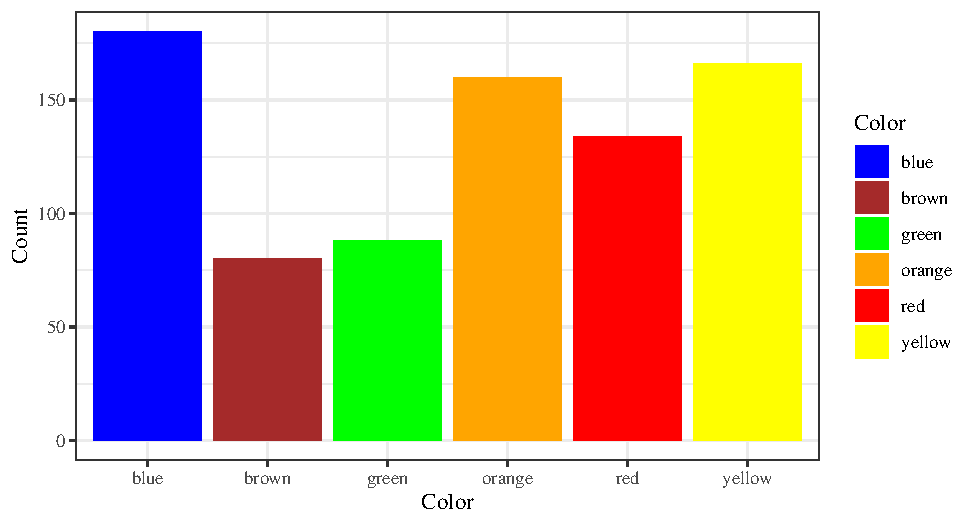
\includegraphics{R-anvisningar_files/figure-latex/unnamed-chunk-153-1} \end{center}

Använd de observerade värdena i kolumnen \texttt{Count} för att testa om alla godisfärger är lika vanliga.
\end{exercise}

Om man har flera klasser kan det vara värdefullt att se vilken klass som bidrar mest till chi-två-värdet. Det kan ge en bild av vilka klasser som är mest speciella. Ett enkelt sätt att göra det på är att spara utfallet av \texttt{chisq.test()} som ett objekt och därifrån hämta \texttt{observed} och \texttt{expected}. Som fortsättning på fotbollsexemplet:

\begin{Shaded}
\begin{Highlighting}[]
\NormalTok{test }\OtherTok{\textless{}{-}} \FunctionTok{chisq.test}\NormalTok{(}\FunctionTok{c}\NormalTok{(}\DecValTok{947}\NormalTok{, }\DecValTok{518}\NormalTok{, }\DecValTok{1285}\NormalTok{), }\AttributeTok{p =} \FunctionTok{c}\NormalTok{(}\FloatTok{0.33}\NormalTok{, }\FloatTok{0.2}\NormalTok{, }\FloatTok{0.47}\NormalTok{))}
\NormalTok{test}\SpecialCharTok{$}\NormalTok{expected}
\end{Highlighting}
\end{Shaded}

\begin{verbatim}
## [1]  907.5  550.0 1292.5
\end{verbatim}

\begin{Shaded}
\begin{Highlighting}[]
\NormalTok{test}\SpecialCharTok{$}\NormalTok{observed}
\end{Highlighting}
\end{Shaded}

\begin{verbatim}
## [1]  947  518 1285
\end{verbatim}

\begin{Shaded}
\begin{Highlighting}[]
\NormalTok{(test}\SpecialCharTok{$}\NormalTok{observed }\SpecialCharTok{{-}}\NormalTok{ test}\SpecialCharTok{$}\NormalTok{expected)}\SpecialCharTok{\^{}}\DecValTok{2} \SpecialCharTok{/}\NormalTok{ test}\SpecialCharTok{$}\NormalTok{expected}
\end{Highlighting}
\end{Shaded}

\begin{verbatim}
## [1] 1.71928375 1.86181818 0.04352031
\end{verbatim}

Antalet hemmavinster (det tredje värdet) ligger när den teoretiska sannolikheten medan de övriga två utfallen ligger längre från.

\begin{exercise}[Udda färger]
Spara testobjektet från testet på M\&M-färger för att se vilka färger som avviker mest från det väntade utfallet.
\end{exercise}

\begin{exercise}[Fågelproportioner som chi-två]
I naturreservatet från en tidigare uppgift tror man fördelningen av tre fåglar (tärnmås, fiskmås och fisktärna) är 50, 30 respektive 20 procent. En studie ger antalen 115, 54 respektive 31. Genomför ett chi-två-test för att testa de antagna andelarna. Är resultatet i linje med de separata testen från den tidigare uppgiften?
\end{exercise}

\begin{exercise}[Udda fåglar]
Spara testobjektet från chi-två-testet för fåglarna för att se vilka fågelarter som avviker mest från det väntade utfallet.
\end{exercise}

\section{Chi-två-test när någon parameter skattas från datan}\label{chi-tvuxe5-test-nuxe4r-nuxe5gon-parameter-skattas-fruxe5n-datan}

(Det här stycket är överkurs och kan läsas översiktligt eller hoppas över.)

I de exempel vi sett hittills har nollhypotesen direkt givit de sannolikheter vi vill testa. Ett annat vanligt fall är att man testar om värdena följer en viss fördelning, men parametervärden i den fördelningen skattas från den insamlade datan. Ta som exempel frågan om antal mål per match följer en poissonfördelning. Hypoteserna ges av

H0: antal mål följer en poissonfördelning,

H1: antal mål följer ej en poissonfördelning.

Här måste vi skatta medelvärdet från datan för att beräkna sannolikheter från fördelningen.

\begin{Shaded}
\begin{Highlighting}[]
\NormalTok{mean\_goals }\OtherTok{\textless{}{-}} \FunctionTok{mean}\NormalTok{(dat\_alls}\SpecialCharTok{$}\NormalTok{hemmamal }\SpecialCharTok{+}\NormalTok{ dat\_alls}\SpecialCharTok{$}\NormalTok{bortamal)}
\NormalTok{mean\_goals}
\end{Highlighting}
\end{Shaded}

\begin{verbatim}
## [1] 3.290182
\end{verbatim}

\begin{Shaded}
\begin{Highlighting}[]
\NormalTok{dat\_goals }\OtherTok{\textless{}{-}}\NormalTok{ dat\_alls }\SpecialCharTok{\%\textgreater{}\%} 
  \FunctionTok{count}\NormalTok{(Mål }\OtherTok{=}\NormalTok{ bortamal }\SpecialCharTok{+}\NormalTok{ hemmamal, }\AttributeTok{name =} \StringTok{"O"}\NormalTok{) }\SpecialCharTok{\%\textgreater{}\%} 
  \FunctionTok{mutate}\NormalTok{(}\AttributeTok{p =} \FunctionTok{dpois}\NormalTok{(Mål, }\AttributeTok{lambda =}\NormalTok{ mean\_goals),}
         \AttributeTok{E =}\NormalTok{ p }\SpecialCharTok{*} \DecValTok{2750}\NormalTok{)}
\NormalTok{dat\_goals}
\end{Highlighting}
\end{Shaded}

\begin{verbatim}
## # A tibble: 13 x 4
##      Mål     O        p       E
##    <dbl> <int>    <dbl>   <dbl>
##  1     0   138 0.0372   102.   
##  2     1   383 0.123    337.   
##  3     2   548 0.202    554.   
##  4     3   542 0.221    608.   
##  5     4   466 0.182    500.   
##  6     5   306 0.120    329.   
##  7     6   183 0.0656   180.   
##  8     7    97 0.0308    84.8  
##  9     8    42 0.0127    34.9  
## 10     9    29 0.00464   12.8  
## 11    10     6 0.00153    4.20 
## 12    11     5 0.000456   1.26 
## 13    12     5 0.000125   0.344
\end{verbatim}

En graf kan illustrera faktiska antal (som punkter) och den skattade poissonfördelningen (som linje).

\begin{exercise}[Målgraf]

Fyll i de saknade delarna i koden nedan för en graf med faktiska antal \texttt{O} som punkter och förväntade antal \texttt{E} som en linje.

\begin{Shaded}
\begin{Highlighting}[]
\FunctionTok{ggplot}\NormalTok{(dat\_goals) }\SpecialCharTok{+}
  \FunctionTok{geom\_point}\NormalTok{(}\FunctionTok{aes}\NormalTok{(}\AttributeTok{x =}\NormalTok{ Mål, }\AttributeTok{y =}\NormalTok{ \_\_\_)) }\SpecialCharTok{+}
  \FunctionTok{geom\_line}\NormalTok{(}\FunctionTok{aes}\NormalTok{(}\AttributeTok{x =}\NormalTok{ Mål, }\AttributeTok{y =}\NormalTok{ \_\_\_))}
\end{Highlighting}
\end{Shaded}

\end{exercise}

De faktiska observationerna är inte så långt från poissonfördelningen.

Ett problem med de förväntade antalen är att några av dem är under 5 - den gräns vi satte för en acceptabel chi-två-approximation. Det vanligaste sättet att hantera det är att slå ihop klasser. Här slås klasser över 9 ihop till en grupp. Det är inte så väsentligt hur det görs här, även om \texttt{ifelse()} kan vara ett nyttigt trick.

\begin{Shaded}
\begin{Highlighting}[]
\NormalTok{dat\_goals\_merged }\OtherTok{\textless{}{-}}\NormalTok{ dat\_goals }\SpecialCharTok{\%\textgreater{}\%} 
  \FunctionTok{mutate}\NormalTok{(Mål }\OtherTok{=} \FunctionTok{ifelse}\NormalTok{(Mål }\SpecialCharTok{\textgreater{}} \DecValTok{9}\NormalTok{, }\DecValTok{10}\NormalTok{, Mål)) }\SpecialCharTok{\%\textgreater{}\%} 
  \FunctionTok{group\_by}\NormalTok{(Mål) }\SpecialCharTok{\%\textgreater{}\%} 
  \FunctionTok{summarise}\NormalTok{(}\AttributeTok{O =} \FunctionTok{sum}\NormalTok{(O),}
            \AttributeTok{p =} \FunctionTok{sum}\NormalTok{(p),}
            \AttributeTok{E =} \FunctionTok{sum}\NormalTok{(E))}
\NormalTok{dat\_goals\_merged}
\end{Highlighting}
\end{Shaded}

\begin{verbatim}
## # A tibble: 11 x 4
##      Mål     O       p      E
##    <dbl> <int>   <dbl>  <dbl>
##  1     0   138 0.0372  102.  
##  2     1   383 0.123   337.  
##  3     2   548 0.202   554.  
##  4     3   542 0.221   608.  
##  5     4   466 0.182   500.  
##  6     5   306 0.120   329.  
##  7     6   183 0.0656  180.  
##  8     7    97 0.0308   84.8 
##  9     8    42 0.0127   34.9 
## 10     9    29 0.00464  12.8 
## 11    10    16 0.00211   5.80
\end{verbatim}

En sista svårighet är antalet frihetsgrader. I ett goodness-of-fit-test ges antalet frihetsgrader av antalet klasser minus antalet skattade parametrar minus 1. I det här fallet har vi nu 11 klasser och vi har skattat en parameter. Vi ska alltså ha 9 frihetsgrader i testet. Funktionen \texttt{chisq.test()} beräknar tyvärr antalet frihetsgrader internt som antalet klasser minus 1, så vi får beräkna chi-två-värde och p-värde på egen hand.

\begin{Shaded}
\begin{Highlighting}[]
\NormalTok{chisq\_value }\OtherTok{\textless{}{-}} \FunctionTok{sum}\NormalTok{((dat\_goals\_merged}\SpecialCharTok{$}\NormalTok{O }\SpecialCharTok{{-}}\NormalTok{ dat\_goals\_merged}\SpecialCharTok{$}\NormalTok{E)}\SpecialCharTok{\^{}}\DecValTok{2} \SpecialCharTok{/}\NormalTok{ dat\_goals\_merged}\SpecialCharTok{$}\NormalTok{E)}
\DecValTok{1} \SpecialCharTok{{-}} \FunctionTok{pchisq}\NormalTok{(chisq\_value, }\AttributeTok{df =} \DecValTok{9}\NormalTok{)}
\end{Highlighting}
\end{Shaded}

\begin{verbatim}
## [1] 6.984746e-12
\end{verbatim}

Chi-två-värdet blir extremt stort och p-värdet väldigt lågt. Nollhypotesen att antalet mål följer en poissonfördelning förkastas.

\section{Bonus. Interaktiva kartor med leaflet}\label{bonus.-interaktiva-kartor-med-leaflet}

Paketet \texttt{leaflet} (\url{https://rstudio.github.io/leaflet/}) kopplar R till leaflet - ett verktyg för interaktiva kartor som ofta använd för kartor online.

\begin{exercise}[Installera leaflet]

Installera och ladda `leaflet genom att fylla i och köra raden nedan.

\begin{Shaded}
\begin{Highlighting}[]
\FunctionTok{install.packages}\NormalTok{(}\StringTok{"leaflet"}\NormalTok{)}
\FunctionTok{library}\NormalTok{(leaflet)}
\end{Highlighting}
\end{Shaded}

\end{exercise}

Som en första kontroll kan vi köra den exempelkod som ges på hemsidan länkad till ovan.

\begin{Shaded}
\begin{Highlighting}[]
\NormalTok{m }\OtherTok{\textless{}{-}} \FunctionTok{leaflet}\NormalTok{() }\SpecialCharTok{\%\textgreater{}\%}
  \FunctionTok{addTiles}\NormalTok{() }\SpecialCharTok{\%\textgreater{}\%}
  \FunctionTok{addMarkers}\NormalTok{(}\AttributeTok{lng =} \FloatTok{174.768}\NormalTok{, }\AttributeTok{lat =} \SpecialCharTok{{-}}\FloatTok{36.852}\NormalTok{, }\AttributeTok{popup=}\StringTok{"The birthplace of R"}\NormalTok{)}
\NormalTok{m}
\end{Highlighting}
\end{Shaded}

På canvassidan finns en excelfil med data tillgänglig på Artportalen - \emph{Artportalen, feromoninventering, 2011-2013.xlsx}. Datan kommer från från ett inventeringsprojekt vid SLU.

\begin{exercise}[Importera datan]

Ladda ner excelfilen och läs in datan med \texttt{read\_excel()} från paketet \texttt{readxl}.

\begin{Shaded}
\begin{Highlighting}[]
\FunctionTok{library}\NormalTok{(readxl)}
\NormalTok{dat\_leaf }\OtherTok{\textless{}{-}} \FunctionTok{read\_excel}\NormalTok{(}\StringTok{"\_\_\_"}\NormalTok{)}
\end{Highlighting}
\end{Shaded}

\end{exercise}

Kartans utseende kan ändras genom att ange en källa och karttyp. Tillgängliga alternativ kan skrivas ut med \texttt{providers}.

\begin{Shaded}
\begin{Highlighting}[]
\FunctionTok{leaflet}\NormalTok{() }\SpecialCharTok{\%\textgreater{}\%} 
  \FunctionTok{addTiles}\NormalTok{() }\SpecialCharTok{\%\textgreater{}\%} 
  \FunctionTok{addProviderTiles}\NormalTok{(providers}\SpecialCharTok{$}\NormalTok{Stamen.Toner)}
\end{Highlighting}
\end{Shaded}

\begin{exercise}[Baskarta]
Skriv ut tillgängliga baskartor med \texttt{providers}. Välj ett alternativ slumpmässigt och ändra koden ovan för att se hur det ser ut.
\end{exercise}

För att lägga till datapunkter kan man använda \texttt{addCircleMarkers()}.

\begin{Shaded}
\begin{Highlighting}[]
\FunctionTok{leaflet}\NormalTok{() }\SpecialCharTok{\%\textgreater{}\%} 
  \FunctionTok{addTiles}\NormalTok{() }\SpecialCharTok{\%\textgreater{}\%} 
  \FunctionTok{addCircleMarkers}\NormalTok{(}\AttributeTok{lng =}\NormalTok{ dat\_leaf}\SpecialCharTok{$}\NormalTok{lng, }\AttributeTok{lat =}\NormalTok{ dat\_leaf}\SpecialCharTok{$}\NormalTok{lat, }\AttributeTok{radius =} \DecValTok{10}\NormalTok{)}
\end{Highlighting}
\end{Shaded}

\begin{exercise}[Cirkelstorlek]
Ändra storleken på cirklarna från \texttt{addCircleMarkers()} genom argumentet \texttt{radius}.
\end{exercise}

Slutligen kan vi lägga till en etikett för år med argumentet \texttt{popup}. Texten kommer upp när man klickar på en punkt.

\begin{Shaded}
\begin{Highlighting}[]
\FunctionTok{leaflet}\NormalTok{() }\SpecialCharTok{\%\textgreater{}\%} 
  \FunctionTok{addTiles}\NormalTok{() }\SpecialCharTok{\%\textgreater{}\%} 
  \FunctionTok{addCircleMarkers}\NormalTok{(}\AttributeTok{lng =}\NormalTok{ dat\_leaf}\SpecialCharTok{$}\NormalTok{lng, }\AttributeTok{lat =}\NormalTok{ dat\_leaf}\SpecialCharTok{$}\NormalTok{lat, }\AttributeTok{radius =} \DecValTok{10}\NormalTok{, }\AttributeTok{popup =}\NormalTok{ dat\_leaf}\SpecialCharTok{$}\NormalTok{Rödlistade)}
\end{Highlighting}
\end{Shaded}

\begin{exercise}[Artnamn]
Ändra i koden ovan för att ange artnamn som popup-text istället för rödlistestatus. Funktionen \texttt{paste()} kan också vara intressant för att ta med mer information i texten: \texttt{paste(dat\_leaf\$Rödlistade,\ dat\_leaf\$Antal)} skulle exempelvis ge både status och antal individer vid den specifika observationen.
\end{exercise}

\chapter{Test för två stickprov}\label{test-fuxf6r-tvuxe5-stickprov}

Datorövning 5 handlar om hypotestest och konfidensintervall för jämförelse av två stickprov. Efter övningen ska vi kunna genomföra och tolka

\begin{itemize}
\item
  t-test för jämförelse av två medelvärden,
\item
  z-test för jämförelse av två proportioner,
\item
  chi-två-test för jämförelse fördelningar mellan två eller flera grupper,
\item
  konfidensintervall för skillnaden mellan två medelvärden eller två proportioner.
\end{itemize}

\section{Repetition av datorövning 4}\label{repetition-av-datoruxf6vning-4}

När man startar en ny R-session bör man ladda de paket man vet kommer behövas med \texttt{library()}. Om paket inte finns installerade måste man först köra \texttt{install.packages()}.

\begin{Shaded}
\begin{Highlighting}[]
\CommentTok{\# install.packages("tidyverse")}
\FunctionTok{library}\NormalTok{(tidyverse)}
\end{Highlighting}
\end{Shaded}

I datorövning 5 tittade vi på tester som inte bygger på normalfördelning: dels tester för proportioner, där varje observation är något av två möjliga utfall; dels tester för kategoridata, där varje observation har ett ufall i någon av flera kategorier.

Proportioner kan testas med ett z-test. Säg att man testar om en doft har en effekt på en insekt, man skickar 20 insekter i ett y-rör och 16 går mot doften. Hypoteserna ges av

\begin{itemize}
\tightlist
\item
  H0: proportionen i populationen är 0.5,
\item
  H1: proportionen i populationen är inte 0.5.
\end{itemize}

I R genomförs ett z-test med \texttt{prop.test()}. Funktionen gör en korrektion som ger ett något bättre test än det man ofta beräknar för hand. Korrektionen kan sättas av med argumentet \texttt{correct}.

\begin{Shaded}
\begin{Highlighting}[]
\FunctionTok{prop.test}\NormalTok{(}\AttributeTok{x =} \DecValTok{16}\NormalTok{, }\AttributeTok{n =} \DecValTok{20}\NormalTok{, }\AttributeTok{p =} \FloatTok{0.5}\NormalTok{, }\AttributeTok{correct =}\NormalTok{ F)}
\end{Highlighting}
\end{Shaded}

\begin{verbatim}
## 
##  1-sample proportions test without continuity correction
## 
## data:  16 out of 20, null probability 0.5
## X-squared = 7.2, df = 1, p-value = 0.00729
## alternative hypothesis: true p is not equal to 0.5
## 95 percent confidence interval:
##  0.5839826 0.9193423
## sample estimates:
##   p 
## 0.8
\end{verbatim}

Ett lågt p-värde tyder på en signifikant skillnad från 0.5.

För att få samma konfidensintervall som det man beräknar för hand kan man använda \texttt{binom.asymp()} från paketet \texttt{binom}.

\begin{Shaded}
\begin{Highlighting}[]
\FunctionTok{library}\NormalTok{(binom)}
\FunctionTok{binom.asymp}\NormalTok{(}\DecValTok{16}\NormalTok{, }\DecValTok{20}\NormalTok{)}
\end{Highlighting}
\end{Shaded}

\begin{verbatim}
##       method  x  n mean     lower     upper
## 1 asymptotic 16 20  0.8 0.6246955 0.9753045
\end{verbatim}

Populationens proportion ligger med 95 procents konfidens mellan 0.62 och 0.98.

Om utfallen är mer än två kategorier kan en hypotes om datans fördelning testas med ett goodness-of-fit-test, vilket är ett slags chi-två-test. Testet bygger på att observerade antal (O) ställs mot förväntade antal (E). I R genomförs ett chi-två-test med \texttt{chisq.test()}. Säg som exempel att man studerar fågelpopulationer genom en observationsstudie. Observerade antal av fyra fågelarter är 102, 53, 75 och 12 och de förväntade andelarna av arterna är 50, 15, 25 och 10 procent. Testets hypoteser ges av

\begin{itemize}
\tightlist
\item
  H0: proportionerna följer den förväntade fördelningen,
\item
  H1: proportionerna följer inte den förväntade fördelningen,
\end{itemize}

och testet ges av

\begin{Shaded}
\begin{Highlighting}[]
\FunctionTok{chisq.test}\NormalTok{(}\FunctionTok{c}\NormalTok{(}\DecValTok{102}\NormalTok{, }\DecValTok{53}\NormalTok{, }\DecValTok{75}\NormalTok{, }\DecValTok{12}\NormalTok{), }\AttributeTok{p =} \FunctionTok{c}\NormalTok{(}\FloatTok{0.5}\NormalTok{, }\FloatTok{0.15}\NormalTok{, }\FloatTok{0.25}\NormalTok{, }\FloatTok{0.1}\NormalTok{))}
\end{Highlighting}
\end{Shaded}

\begin{verbatim}
## 
##  Chi-squared test for given probabilities
## 
## data:  c(102, 53, 75, 12)
## X-squared = 20.292, df = 3, p-value = 0.0001477
\end{verbatim}

Ett lågt p-värde tyder på att de antagna proportionerna inte stämmer. Antalet frihetsgrader ges i ett chi-två-test av antalet klasser minus antalet skattade parametrar minus ett. I det här fallet finns fyra klasser och ingen skattad parameter.

\section{Två stickprov och normalfördelad data}\label{tvuxe5-stickprov-och-normalfuxf6rdelad-data}

Vid normalfördelad data från två stickprov eller grupper vill vi nästan alltid testa om populationerna har samma medelvärde. Det kan också ses som att vi testar om differensen mellan medelvärdena är noll. Vi skiljer mellan två fall: \emph{matchade stickprov} - där varje observation i den ena gruppen är \emph{kopplad} till en observation i den andra gruppen; och \emph{oberoende stickprov} - där det inte finns någon sådan koppling mellan stickproven. Typiska exempel på matchade stickprov är när man mäter samma individ för och efter en behandling och syskonstudier där ett syskon får en behandling och den andra en annan behandling.

\subsection{t-test för två matchade stickprov}\label{t-test-fuxf6r-tvuxe5-matchade-stickprov}

Vid matchade stickprov kan varje observation i en behandlingsgrupp paras med en observation i den andra gruppen. Själva testet är ett t-test för \emph{ett} stickprov på differensserien beräknat från varje par. I R kan man antingen beräkna den differensserien eller använda \texttt{t.test()} med två dataserier och argumentet för parvisa observationer satt till sant, \texttt{paired\ =\ T}.
Som exempel ges följande data från en studie på äpple, där trädhöjd mätts före och efter en näringsbehandling.

\begin{Shaded}
\begin{Highlighting}[]
\NormalTok{dat\_apple }\OtherTok{\textless{}{-}} \FunctionTok{tibble}\NormalTok{(}\AttributeTok{Tree =} \DecValTok{1}\SpecialCharTok{:}\DecValTok{4}\NormalTok{, }
              \AttributeTok{Before =} \FunctionTok{c}\NormalTok{(}\DecValTok{48}\NormalTok{, }\DecValTok{43}\NormalTok{, }\DecValTok{30}\NormalTok{, }\DecValTok{47}\NormalTok{), }
              \AttributeTok{After =} \FunctionTok{c}\NormalTok{(}\DecValTok{51}\NormalTok{, }\DecValTok{44}\NormalTok{, }\DecValTok{42}\NormalTok{, }\DecValTok{54}\NormalTok{))}
\NormalTok{dat\_apple}
\end{Highlighting}
\end{Shaded}

\begin{verbatim}
## # A tibble: 4 x 3
##    Tree Before After
##   <int>  <dbl> <dbl>
## 1     1     48    51
## 2     2     43    44
## 3     3     30    42
## 4     4     47    54
\end{verbatim}

Datan kan illustreras med ett punktdiagram där en linje binder samman paret. För att enkelt skapa grafen i \texttt{ggplot2} kan man först omstrukturera datan till lång form genom \texttt{pivot\_longer}.

\begin{Shaded}
\begin{Highlighting}[]
\NormalTok{dat\_long }\OtherTok{\textless{}{-}}\NormalTok{ dat\_apple }\SpecialCharTok{\%\textgreater{}\%} \FunctionTok{pivot\_longer}\NormalTok{(}\SpecialCharTok{{-}}\NormalTok{Tree, }\AttributeTok{names\_to =} \StringTok{"Time"}\NormalTok{, }\AttributeTok{values\_to =} \StringTok{"Height"}\NormalTok{)}
\NormalTok{dat\_long}
\end{Highlighting}
\end{Shaded}

\begin{verbatim}
## # A tibble: 8 x 3
##    Tree Time   Height
##   <int> <chr>   <dbl>
## 1     1 Before     48
## 2     1 After      51
## 3     2 Before     43
## 4     2 After      44
## 5     3 Before     30
## 6     3 After      42
## 7     4 Before     47
## 8     4 After      54
\end{verbatim}

\begin{exercise}[Äppelgraf]

Fyll i kodstycket nedan för en graf av äppeldatan. Axlarna ges av \texttt{Time} och \texttt{Height}. Två observationer kan kopplas genom att sätta \texttt{Tree} som grupp.

\begin{Shaded}
\begin{Highlighting}[]
\FunctionTok{ggplot}\NormalTok{(dat\_long, }\FunctionTok{aes}\NormalTok{(\_\_\_, \_\_\_, }\AttributeTok{group =}\NormalTok{ \_\_\_)) }\SpecialCharTok{+}
  \FunctionTok{geom\_point}\NormalTok{() }\SpecialCharTok{+}
  \FunctionTok{geom\_line}\NormalTok{()}
\end{Highlighting}
\end{Shaded}

\end{exercise}

För att testa för skillnad före och efter behandling sätter vi upp hypoteser

\begin{itemize}
\tightlist
\item
  H0: mu före behandling är lika med mu efter behandling
\item
  H1: mu före behandling är skild från mu efter behandling
\end{itemize}

Testet kan antingen utföras som ett enkelt t-test på differensserien

\begin{Shaded}
\begin{Highlighting}[]
\FunctionTok{t.test}\NormalTok{(dat\_apple}\SpecialCharTok{$}\NormalTok{Before }\SpecialCharTok{{-}}\NormalTok{ dat\_apple}\SpecialCharTok{$}\NormalTok{After)}
\end{Highlighting}
\end{Shaded}

\begin{verbatim}
## 
##  One Sample t-test
## 
## data:  dat_apple$Before - dat_apple$After
## t = -2.3681, df = 3, p-value = 0.09868
## alternative hypothesis: true mean is not equal to 0
## 95 percent confidence interval:
##  -13.477405   1.977405
## sample estimates:
## mean of x 
##     -5.75
\end{verbatim}

eller som ett t-test för två stickprov där man särskilt anger att datan är parad

\begin{Shaded}
\begin{Highlighting}[]
\FunctionTok{t.test}\NormalTok{(dat\_apple}\SpecialCharTok{$}\NormalTok{Before, dat\_apple}\SpecialCharTok{$}\NormalTok{After, }\AttributeTok{paired =}\NormalTok{ T)}
\end{Highlighting}
\end{Shaded}

\begin{verbatim}
## 
##  Paired t-test
## 
## data:  dat_apple$Before and dat_apple$After
## t = -2.3681, df = 3, p-value = 0.09868
## alternative hypothesis: true mean difference is not equal to 0
## 95 percent confidence interval:
##  -13.477405   1.977405
## sample estimates:
## mean difference 
##           -5.75
\end{verbatim}

För bägge alternativen måste datan vara ordnad så att de två vektorerna matchar varandra parvis. Ett p-värde på \(0.0987\) ger att man inte förkastar vid en signifikansnivå på fem procent. Vi drar därmed slutsatsen att det inte finns någon signifikant skillnad före och efter behandling.

\begin{exercise}[Ensidigt test]
Gör ett tillägg till ett av kodstyckena med \texttt{t.test()} för att beräkna ett ensidigt test med mothypotesen att träden ökar i höjd efter behandling. Hjälpsidan för \texttt{t.test()} kan tas fram genom att köra \texttt{?t.test()}.
\end{exercise}

Konfidensintervallet beräknas från differenserna på samma sätt som vid ett stickprov med normalfördelad data. Tolkningen liknar den för ett stickprov: med 95 procents konfidens ligger den sanna skillnaden i medelvärden i intervallet.

\begin{exercise}[Lökimport]

Åtta monoglukosidmätningar på lök samlas in från fyra konventionella och fyra ekologiska ordlare. Resultatet finns i fliken \emph{Lökfärg} i excelfilen \emph{Uppgiftsdata.xlsx} på canvassidan. Ladda ner filen och importera datan genom att fylla i raden nedan.

\begin{Shaded}
\begin{Highlighting}[]
\FunctionTok{library}\NormalTok{(readxl)}
\NormalTok{dat\_onion }\OtherTok{\textless{}{-}} \FunctionTok{read\_excel}\NormalTok{(}\StringTok{"\_\_\_\_"}\NormalTok{, }\AttributeTok{sheet =} \StringTok{"Lökfärg"}\NormalTok{)}
\CommentTok{\# dat\_onion \textless{}{-} read\_csv("https://raw.githubusercontent.com/adamflr/ST0060/main/Data/Uppgiftsdata/Uppgift\_L\%C3\%B6kf\%C3\%A4rg.csv") \# Alternativ lösning}
\end{Highlighting}
\end{Shaded}

\end{exercise}

\begin{exercise}[Lökgraf]
Fyll i stycket nedan för en graf av lökdatan från föregående uppgift.

\begin{Shaded}
\begin{Highlighting}[]
\NormalTok{dat\_long }\OtherTok{\textless{}{-}}\NormalTok{ dat\_onion }\SpecialCharTok{\%\textgreater{}\%} 
  \FunctionTok{pivot\_longer}\NormalTok{(}\SpecialCharTok{{-}}\NormalTok{Odlare, }\AttributeTok{names\_to =} \StringTok{"Odlingstyp"}\NormalTok{, }\AttributeTok{values\_to =} \StringTok{"Utfall"}\NormalTok{)}
\NormalTok{dat\_long}

\FunctionTok{ggplot}\NormalTok{(dat\_long, }\FunctionTok{aes}\NormalTok{(\_\_\_, \_\_\_, }\AttributeTok{group =}\NormalTok{ Odlare)) }\SpecialCharTok{+}
  \FunctionTok{geom\_point}\NormalTok{() }\SpecialCharTok{+}
  \FunctionTok{geom\_line}\NormalTok{()}
\end{Highlighting}
\end{Shaded}

Tyder grafen på någon skillnad mellan odlingstyper?
\end{exercise}

\begin{exercise}[Löktest]
Använd lökdatan i föregående uppgift för att testa om det finns en signifikant skillnad mellan konventionell och ekologisk.
Formulera hypoteser och genomför testet med \texttt{t.test()}. Lös gärna uppgiften med miniräknare först.
\end{exercise}

\subsection{t-test för två oberoende stickprov}\label{t-test-fuxf6r-tvuxe5-oberoende-stickprov}

Ett t-test för två oberoende stickprov testar om två populationsmedelvärden är lika. Ta som exempel följande data på jordgubbsskörd vid två olika näringsbehandlingar (A och B). Här är stickproven inte matchade - det finns \textbf{ingen} direkt koppling mellan en observation i den ena behandlingsgruppen till någon observation i den andra.

\begin{Shaded}
\begin{Highlighting}[]
\NormalTok{dat\_berry }\OtherTok{\textless{}{-}} \FunctionTok{data.frame}\NormalTok{(}\AttributeTok{Behandling =} \FunctionTok{c}\NormalTok{(}\StringTok{"A"}\NormalTok{, }\StringTok{"A"}\NormalTok{, }\StringTok{"A"}\NormalTok{, }\StringTok{"A"}\NormalTok{, }\StringTok{"B"}\NormalTok{, }\StringTok{"B"}\NormalTok{, }\StringTok{"B"}\NormalTok{, }\StringTok{"B"}\NormalTok{),}
              \AttributeTok{Vikt =} \FunctionTok{c}\NormalTok{(}\DecValTok{40}\NormalTok{, }\FloatTok{48.2}\NormalTok{, }\FloatTok{39.2}\NormalTok{, }\FloatTok{47.9}\NormalTok{, }\FloatTok{57.5}\NormalTok{, }\FloatTok{61.5}\NormalTok{, }\DecValTok{58}\NormalTok{, }\FloatTok{66.5}\NormalTok{))}
\NormalTok{dat\_berry}
\end{Highlighting}
\end{Shaded}

\begin{verbatim}
##   Behandling Vikt
## 1          A 40.0
## 2          A 48.2
## 3          A 39.2
## 4          A 47.9
## 5          B 57.5
## 6          B 61.5
## 7          B 58.0
## 8          B 66.5
\end{verbatim}

Datan kan illustreras med ett enkelt punktdiagram.

\begin{Shaded}
\begin{Highlighting}[]
\FunctionTok{ggplot}\NormalTok{(dat\_berry, }\FunctionTok{aes}\NormalTok{(Behandling, Vikt)) }\SpecialCharTok{+}
  \FunctionTok{geom\_point}\NormalTok{()}
\end{Highlighting}
\end{Shaded}

\begin{center}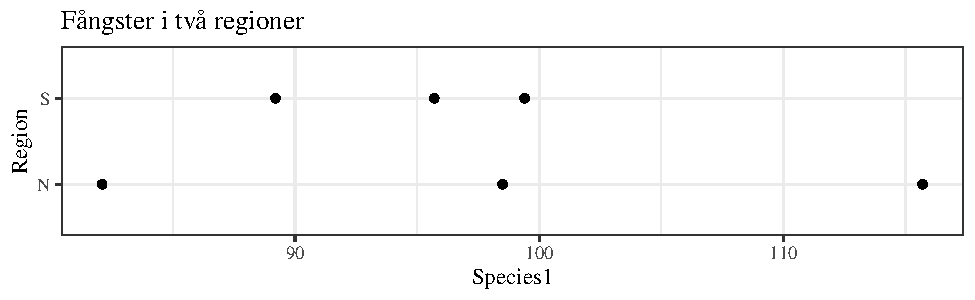
\includegraphics{R-anvisningar_files/figure-latex/unnamed-chunk-177-1} \end{center}

Ett t-test för två oberoende stickprov har nollhypotesen att grupperna har samma populationsmedelvärde och alternativhypotesen att populationsmedelvärdena är skilda (för det tvåsidiga fallet):

\begin{itemize}
\tightlist
\item
  H0: mu\_A är lika med mu\_B
\item
  H1: mu\_A är ej lika med mu\_B
\end{itemize}

Testet kan utföras i R genom funktionen \texttt{t.test()}. Data kan antingen anges som en formel med dess data \texttt{Vikt\ \textasciitilde{}\ Behandling,\ data\ =\ dat\_berry} (vilket man kan läsa som \emph{vikt uppdelat efter behandling}) eller som två skilda vektorer. Det förra alternativet är oftast enklare om man har datan på lång form - med en kolumn som anger grupp (i exemplet \emph{Behandling}) och en kolumn som anger utfallsvärdet (i exemplet \emph{Vikt}).

För formen med formel ger det

\begin{Shaded}
\begin{Highlighting}[]
\CommentTok{\# Formelskrivning}
\FunctionTok{t.test}\NormalTok{(Vikt }\SpecialCharTok{\textasciitilde{}}\NormalTok{ Behandling, }\AttributeTok{data =}\NormalTok{ dat\_berry, }\AttributeTok{var.equal =}\NormalTok{ T)}
\end{Highlighting}
\end{Shaded}

\begin{verbatim}
## 
##  Two Sample t-test
## 
## data:  Vikt by Behandling
## t = -5.3157, df = 6, p-value = 0.001803
## alternative hypothesis: true difference in means between group A and group B is not equal to 0
## 95 percent confidence interval:
##  -24.898417  -9.201583
## sample estimates:
## mean in group A mean in group B 
##          43.825          60.875
\end{verbatim}

och för formen med vektorer

\begin{Shaded}
\begin{Highlighting}[]
\CommentTok{\# Två separata vektorer}
\DocumentationTok{\#\# Filtrera ut data där behandling är A}
\NormalTok{Vikt\_A }\OtherTok{\textless{}{-}}\NormalTok{ dat\_berry}\SpecialCharTok{$}\NormalTok{Vikt[dat\_berry}\SpecialCharTok{$}\NormalTok{Behandling }\SpecialCharTok{==} \StringTok{"A"}\NormalTok{]}

\DocumentationTok{\#\# Filtrera ut data där behandling är B}
\NormalTok{Vikt\_B }\OtherTok{\textless{}{-}}\NormalTok{ dat\_berry}\SpecialCharTok{$}\NormalTok{Vikt[dat\_berry}\SpecialCharTok{$}\NormalTok{Behandling }\SpecialCharTok{==} \StringTok{"B"}\NormalTok{]}

\FunctionTok{t.test}\NormalTok{(Vikt\_A, Vikt\_B, }\AttributeTok{var.equal =}\NormalTok{ T)}
\end{Highlighting}
\end{Shaded}

\begin{verbatim}
## 
##  Two Sample t-test
## 
## data:  Vikt_A and Vikt_B
## t = -5.3157, df = 6, p-value = 0.001803
## alternative hypothesis: true difference in means is not equal to 0
## 95 percent confidence interval:
##  -24.898417  -9.201583
## sample estimates:
## mean of x mean of y 
##    43.825    60.875
\end{verbatim}

Argumentet \texttt{var.equal\ =\ T} används för att beräkna testet där gruppernas varianser antas vara lika. Grundinställningen är testet där varianser inte antas vara lika, så \texttt{t.test(Vikt\ \textasciitilde{}\ Behandling,\ data\ =\ dat)} ger ett lite annat resultat.

\begin{exercise}[Ej lika varianser]
Vilka resultatvärden ändras i utskriften om man sätter \texttt{var.equal\ =\ F}?
\end{exercise}

Testet ger ett p-värde på \(0.0018\), vilket leder till att nollhypotesen förkastas på enprocentsnivån. Detta tyder på att det finns en viktskillnad mellan behandlingarna. Utskriften ger också ett 95-procentigt konfidensintervall på \((-24.898, -9.202)\). Tolkningen är att skillnaden mellan populationsmedelvärden ligger i intervallet med 95 procents konfidens. Notera att värdet noll inte ligger i intervallet.

\begin{exercise}[Ensidigt test]

Gör lämpliga tillägg till kodstycket nedan för att göra ett ensidigt test (om B ger högre vikt än A).

\begin{Shaded}
\begin{Highlighting}[]
\FunctionTok{t.test}\NormalTok{(Vikt }\SpecialCharTok{\textasciitilde{}}\NormalTok{ Behandling, }\AttributeTok{data =}\NormalTok{ dat\_berry, }\AttributeTok{var.equal =}\NormalTok{ T, }\AttributeTok{alternative =} \StringTok{"two.sided"}\NormalTok{)}
\end{Highlighting}
\end{Shaded}

\end{exercise}

Om man har fler än två grupper kan man vilja göra parvisa t-test - alltså ett t-test för varje par av grupper.
Ett exempel på funktionen \texttt{pairwise.t.test()} ges nedan. Funktionen bygger på att datan är i \emph{lång} form, med en kolumn som anger det numeriska utfallet och en kolumn som anger behandlingen.

\begin{Shaded}
\begin{Highlighting}[]
\FunctionTok{pairwise.t.test}\NormalTok{(dat\_berry}\SpecialCharTok{$}\NormalTok{Vikt, dat\_berry}\SpecialCharTok{$}\NormalTok{Behandling, }\AttributeTok{p.adjust.method =} \StringTok{"none"}\NormalTok{, }\AttributeTok{pool.sd =}\NormalTok{ F)}
\end{Highlighting}
\end{Shaded}

\begin{verbatim}
## 
##  Pairwise comparisons using t tests with non-pooled SD 
## 
## data:  dat_berry$Vikt and dat_berry$Behandling 
## 
##   A    
## B 0.002
## 
## P value adjustment method: none
\end{verbatim}

\emph{Matchade} observationer kan också kallas \emph{parade} (eng. paired) så se upp med terminologin. Funktionen \texttt{pairwise.t.test()} för \emph{parvisa jämförelse} mellan behandlingar, men testerna är t-test för oberoende stickprov.

\begin{exercise}[Ekorrdata]

I en undersökning av hur den europeiska ekorren (Sciurus vulgaris) förändras i vikt under övervintring mäts 7 slumpmässigt valda ekorrar före och 5 slumpmässigt valda ekorrar efter övervintring. Datan finns tillgänglig i excelfilen \emph{Uppgiftsdata.xlsx} på canvassidan, i fliken \emph{Ekorrar}. Ladda ner filen och fyll i stycket nedan för att importera datan.

\begin{Shaded}
\begin{Highlighting}[]
\NormalTok{dat\_sq }\OtherTok{\textless{}{-}} \FunctionTok{read\_excel}\NormalTok{(}\StringTok{"\_\_\_"}\NormalTok{, }\AttributeTok{sheet =} \StringTok{"Ekorrar"}\NormalTok{)}
\NormalTok{dat\_sq}

\CommentTok{\# dat\_sq \textless{}{-} read\_csv("https://raw.githubusercontent.com/adamflr/ST0060/main/Data/Uppgiftsdata/Uppgift\_Ekorrar.csv") \# Alternativ lösning}
\end{Highlighting}
\end{Shaded}

\end{exercise}

\begin{exercise}[Ekorrgraf]
Fyll i följande stycke för en lämplig graf för att jämföra mätningarna före och mätningarna efter.

\begin{Shaded}
\begin{Highlighting}[]
\FunctionTok{ggplot}\NormalTok{(dat\_sq, }\FunctionTok{aes}\NormalTok{(}\AttributeTok{x =}\NormalTok{ \_\_\_, }\AttributeTok{y =}\NormalTok{ \_\_\_)) }\SpecialCharTok{+}
  \FunctionTok{\_\_\_}\NormalTok{()}
\end{Highlighting}
\end{Shaded}

Finns det någon synlig viktskillnad?
\end{exercise}

\begin{exercise}[Ekorrtest]

Genomför ett t-test för två oberoende stickprov på ekorrdatan genom att fylla i kodstycket nedan. Formulera tydliga hypoteser och dra en klar slutsats.

\begin{Shaded}
\begin{Highlighting}[]
\FunctionTok{t.test}\NormalTok{(\_\_\_ }\SpecialCharTok{\textasciitilde{}}\NormalTok{ \_\_\_, }\AttributeTok{data =}\NormalTok{ dat\_sq, }\AttributeTok{var.equal =}\NormalTok{ \_\_\_)}
\end{Highlighting}
\end{Shaded}

\end{exercise}

\begin{exercise}[Ekorrdesign]
Ett problem med att mäta skilda individer före och efter övervintring är att det kan finnas en stor skillnad i vikt mellan individuella ekorrar. Kan man lägga upp försöket på ett sätt som reducerar det problemet?
\end{exercise}

\section{z-test och konfidensintervall för två proportioner}\label{z-test-och-konfidensintervall-fuxf6r-tvuxe5-proportioner}

Om man vill jämföra två proportioner kan man använda z-testet för två stickprov. Säg till exempel att man har två sorter av någon planta och vill se hur stor proportion som är infekterad av bladmögel. I den ena gruppen (sort A) är 17 av 50 infektera och i den andra (sort B) är 26 av 60 infekterade. Testets hypoteser är i det tvåsidiga fallet

\begin{itemize}
\tightlist
\item
  H0: proportion A är lika med proportion B
\item
  H1: proportion A är skild från proportion B
\end{itemize}

I R kan testet genomföras med \texttt{prop.test}-funktionen. Funktionens första argument är antalen infekterade, som en vektor med två värden, och dess andra argument är totalerna. Likt testet med ett stickprov finns en möjlighet att göra en kontinuitetskorrektion med \texttt{correct}-argumentet. För att få samma resultat som räkning för hand anger vi att korrektion inte ska göras med \texttt{correct\ =\ F}.

\begin{Shaded}
\begin{Highlighting}[]
\FunctionTok{prop.test}\NormalTok{(}\FunctionTok{c}\NormalTok{(}\DecValTok{17}\NormalTok{, }\DecValTok{26}\NormalTok{), }\FunctionTok{c}\NormalTok{(}\DecValTok{50}\NormalTok{, }\DecValTok{60}\NormalTok{), }\AttributeTok{correct =}\NormalTok{ F)}
\end{Highlighting}
\end{Shaded}

\begin{verbatim}
## 
##  2-sample test for equality of proportions without continuity correction
## 
## data:  c(17, 26) out of c(50, 60)
## X-squared = 0.9978, df = 1, p-value = 0.3178
## alternative hypothesis: two.sided
## 95 percent confidence interval:
##  -0.27488771  0.08822105
## sample estimates:
##    prop 1    prop 2 
## 0.3400000 0.4333333
\end{verbatim}

Notera att funktionen inte ger ett z-värde utan ett \(\chi^2\)-värde (utskrivet \texttt{X-squared}). Det beror på att funktionen beräknar z-testet som ett likvärdigt \(\chi^2\)-test. Det z-värde man får om man genomför testet som ett z-test är detsamma som roten ur utskriftens \(\chi^2\)-värde. Testet ger ett högt p-värde på 0.32 vilket innebär att nollhypotesen inte förkastas: det finns ingen signifikant skillnad i infektionsproportion.

Funktionen \texttt{prop.test()} ger också en utskrift av konfidensintervallet. Tolkning är att skillnaden i proportioner mellan populationerna ligger i intervallet med 95 procents konfidens. Notera att nollan ingår i intervallet.

\begin{exercise}[Lämplig approximation?]
Z-test bygger på en normalapproximation. Som tumregel för när approximationen är rimlig används ofta att n * p * (1 - p) ska vara större än 10 för bägge stickproven. Gör beräkningen för datan i exemplet (17 av 50 respektive 26 av 60).
\end{exercise}

\begin{exercise}[Burfågel]
Det finns en förvånansvärt stor mängd studier på kopplingen mellan innehav av burfågel och lungcancer. En sådan studie (Kohlmeier et al 1992) ger följande antal för burfågelägande och lungcancer.

\begin{Shaded}
\begin{Highlighting}[]
\NormalTok{dat\_bird }\OtherTok{\textless{}{-}} \FunctionTok{data.frame}\NormalTok{(Burfågel }\OtherTok{=} \FunctionTok{c}\NormalTok{(}\StringTok{"Burfågel"}\NormalTok{, }\StringTok{"Ej\_burfågel"}\NormalTok{),}
              \AttributeTok{Lungcancer =} \FunctionTok{c}\NormalTok{(}\DecValTok{98}\NormalTok{, }\DecValTok{141}\NormalTok{),}
              \AttributeTok{Ej\_lungcancer =} \FunctionTok{c}\NormalTok{(}\DecValTok{101}\NormalTok{, }\DecValTok{328}\NormalTok{))}
\NormalTok{dat\_bird}
\end{Highlighting}
\end{Shaded}

\begin{verbatim}
##      Burfågel Lungcancer Ej_lungcancer
## 1    Burfågel         98           101
## 2 Ej_burfågel        141           328
\end{verbatim}

Datan tyder på att människor med burfågel har en förhöjd risk att drabbas av lungcancer. Genomför ett z-test för att se om andelen burfågelägare än densamma i de två patientgrupperna.

\begin{Shaded}
\begin{Highlighting}[]
\FunctionTok{prop.test}\NormalTok{(}\AttributeTok{x =} \FunctionTok{c}\NormalTok{(\_\_\_, \_\_\_), }\AttributeTok{n =} \FunctionTok{c}\NormalTok{(\_\_\_, \_\_\_), }\AttributeTok{correct =}\NormalTok{ F)}
\end{Highlighting}
\end{Shaded}

Genomför ett z-test för att se om andelen cancerdrabbade är densamma i de två burfågelsgrupperna. Hur förhåller sig p-värdena i de bägge testerna till varandra?

\begin{Shaded}
\begin{Highlighting}[]
\FunctionTok{prop.test}\NormalTok{(}\AttributeTok{x =} \FunctionTok{c}\NormalTok{(\_\_\_, \_\_\_), }\AttributeTok{n =} \FunctionTok{c}\NormalTok{(\_\_\_, \_\_\_), }\AttributeTok{correct =}\NormalTok{ F)}
\end{Highlighting}
\end{Shaded}

Finns det någon industri som kan ha ett intresse av att finansiera forskning som söker alternativa riskfaktorer för lungcancer?
\end{exercise}

\section{Chi-två-test för korstabeller}\label{chi-tvuxe5-test-fuxf6r-korstabeller}

Data med två kategoriska variabler kan presenteras med en korstabell. Ta som (ett något deppigt) exempel överlevnadsdata från Titanic. Datan finns tillgänglig i R som \texttt{Titanic}. I detta fall ges överlevnad filtrerad på vuxna män, uppdelat efter klass.

\begin{Shaded}
\begin{Highlighting}[]
\NormalTok{dat\_titanic }\OtherTok{\textless{}{-}}\NormalTok{ Titanic }\SpecialCharTok{\%\textgreater{}\%} \FunctionTok{data.frame}\NormalTok{() }\SpecialCharTok{\%\textgreater{}\%} \FunctionTok{filter}\NormalTok{(Sex }\SpecialCharTok{==} \StringTok{"Male"}\NormalTok{, Age }\SpecialCharTok{==} \StringTok{"Adult"}\NormalTok{)}
\NormalTok{dat\_titanic}
\end{Highlighting}
\end{Shaded}

\begin{verbatim}
##   Class  Sex   Age Survived Freq
## 1   1st Male Adult       No  118
## 2   2nd Male Adult       No  154
## 3   3rd Male Adult       No  387
## 4  Crew Male Adult       No  670
## 5   1st Male Adult      Yes   57
## 6   2nd Male Adult      Yes   14
## 7   3rd Male Adult      Yes   75
## 8  Crew Male Adult      Yes  192
\end{verbatim}

En korstabell kan konstrueras med \texttt{pivot\_wider}.

\begin{Shaded}
\begin{Highlighting}[]
\NormalTok{dat\_wide }\OtherTok{\textless{}{-}}\NormalTok{ dat\_titanic }\SpecialCharTok{\%\textgreater{}\%} 
  \FunctionTok{pivot\_wider}\NormalTok{(}\AttributeTok{names\_from =}\NormalTok{ Survived, }\AttributeTok{values\_from =}\NormalTok{ Freq)}
\NormalTok{dat\_wide}
\end{Highlighting}
\end{Shaded}

\begin{verbatim}
## # A tibble: 4 x 5
##   Class Sex   Age      No   Yes
##   <fct> <fct> <fct> <dbl> <dbl>
## 1 1st   Male  Adult   118    57
## 2 2nd   Male  Adult   154    14
## 3 3rd   Male  Adult   387    75
## 4 Crew  Male  Adult   670   192
\end{verbatim}

Datan tyder på att överlevnad är beroende av klass. Datan kan illustreras med uppdelade staplar

\begin{Shaded}
\begin{Highlighting}[]
\FunctionTok{ggplot}\NormalTok{(dat\_titanic, }\FunctionTok{aes}\NormalTok{(Class, Freq, }\AttributeTok{fill =}\NormalTok{ Survived)) }\SpecialCharTok{+}
  \FunctionTok{geom\_col}\NormalTok{(}\AttributeTok{position =} \FunctionTok{position\_fill}\NormalTok{(), }\AttributeTok{color =} \StringTok{"black"}\NormalTok{) }\SpecialCharTok{+}
  \FunctionTok{scale\_fill\_manual}\NormalTok{(}\AttributeTok{values =} \FunctionTok{c}\NormalTok{(}\StringTok{"red4"}\NormalTok{, }\StringTok{"white"}\NormalTok{))}
\end{Highlighting}
\end{Shaded}

\begin{center}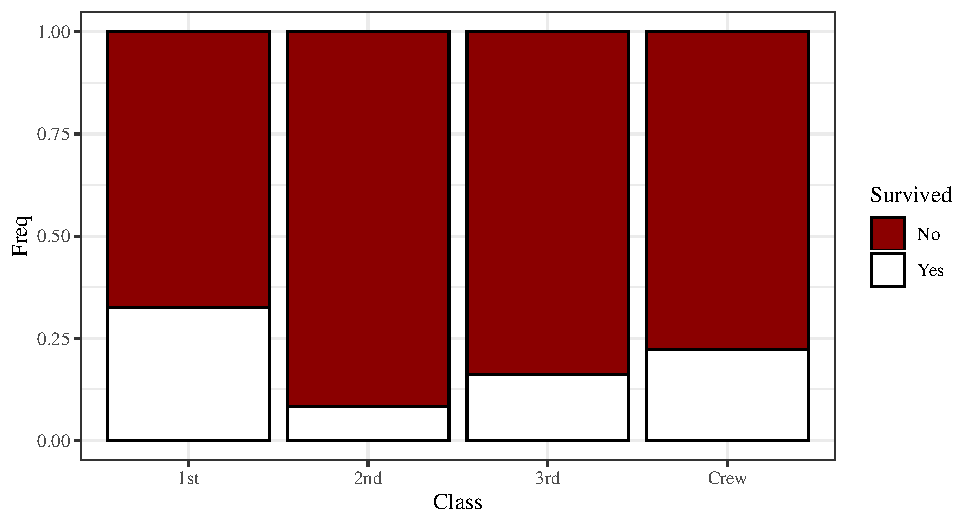
\includegraphics{R-anvisningar_files/figure-latex/unnamed-chunk-191-1} \end{center}

Argumentet \texttt{position} i \texttt{geom\_bar} används för att skapa proportionella staplar.

Ett chi-två-test på en korstabell har nollhypotesen att det inte finns något samband mellan variabeln för rader och variabeln för kolumner. Antal frihetsgrader ges av antal rader minus ett gånger antal kolumner minus ett. Testet kan enkelt göras med \texttt{chisq.test()}. Som ingångsvärde kan man plocka ut kolumnerna med numeriska värden genom hakparenteser.

\begin{Shaded}
\begin{Highlighting}[]
\NormalTok{dat\_wide[, }\DecValTok{4}\SpecialCharTok{:}\DecValTok{5}\NormalTok{] }\CommentTok{\# De två numeriska kolumnerna}
\end{Highlighting}
\end{Shaded}

\begin{verbatim}
## # A tibble: 4 x 2
##      No   Yes
##   <dbl> <dbl>
## 1   118    57
## 2   154    14
## 3   387    75
## 4   670   192
\end{verbatim}

\begin{Shaded}
\begin{Highlighting}[]
\FunctionTok{chisq.test}\NormalTok{(dat\_wide[, }\DecValTok{4}\SpecialCharTok{:}\DecValTok{5}\NormalTok{])}
\end{Highlighting}
\end{Shaded}

\begin{verbatim}
## 
##  Pearson's Chi-squared test
## 
## data:  dat_wide[, 4:5]
## X-squared = 37.988, df = 3, p-value = 2.843e-08
\end{verbatim}

Utskriften ger teststorheten, antal frihetsgrader, och p-värdet. I det här fallet är p-värdet mycket litet och slutsatsen blir att nollhypotesen förkastas - det finns ett samband mellan klass och överlevnad. Antalet frihetsgrader ges av antalet rader minus ett gånger antalet kolumner minus ett (här (4-1) * (2-1) = 3).

Chi-två-testet är ett asymptotiskt test - dess egenskaper är beroende av \emph{stora} stickprov. Som gräns för storleken används ofta att samtliga förväntade antal ska vara större än 5. Funktionen ger en varning om förväntade värden är små. En möjlig lösning i sådana fall är att slå ihop klasser.

\begin{Shaded}
\begin{Highlighting}[]
\NormalTok{test\_result }\OtherTok{\textless{}{-}} \FunctionTok{chisq.test}\NormalTok{(dat\_wide[, }\DecValTok{4}\SpecialCharTok{:}\DecValTok{5}\NormalTok{])}
\NormalTok{test\_result}\SpecialCharTok{$}\NormalTok{expected }\CommentTok{\# Samtliga förväntade värden över 5}
\end{Highlighting}
\end{Shaded}

\begin{verbatim}
##            No       Yes
## [1,] 139.5171  35.48290
## [2,] 133.9364  34.06359
## [3,] 368.3251  93.67487
## [4,] 687.2214 174.77864
\end{verbatim}

Om detta krav inte är uppfyllt skriver funktionen ut en varning.

\begin{exercise}[Ogiltig approximation]

Ta följande lilla korstabell och kör \texttt{chisq.test()} för att få ett felmeddelande.

\begin{Shaded}
\begin{Highlighting}[]
\NormalTok{dat }\OtherTok{\textless{}{-}} \FunctionTok{matrix}\NormalTok{(}\FunctionTok{c}\NormalTok{(}\DecValTok{4}\NormalTok{,}\DecValTok{2}\NormalTok{,}\DecValTok{5}\NormalTok{,}\DecValTok{1}\NormalTok{), }\DecValTok{2}\NormalTok{)}
\NormalTok{dat}
\end{Highlighting}
\end{Shaded}

\begin{verbatim}
##      [,1] [,2]
## [1,]    4    5
## [2,]    2    1
\end{verbatim}

\end{exercise}

\begin{exercise}[Burfågeln återvänder]

En svensk studie på koppling mellan burfågel och lungcancer (Modigh et al, 1996) ger följande antal (för män).

\begin{Shaded}
\begin{Highlighting}[]
\NormalTok{dat\_bird\_swe }\OtherTok{\textless{}{-}} \FunctionTok{data.frame}\NormalTok{(Burfågel }\OtherTok{=} \FunctionTok{c}\NormalTok{(}\StringTok{"Burfågel"}\NormalTok{, }\StringTok{"Ej\_burfågel"}\NormalTok{),}
              \AttributeTok{Lungcancer =} \FunctionTok{c}\NormalTok{(}\DecValTok{108}\NormalTok{, }\DecValTok{144}\NormalTok{),}
              \AttributeTok{Ej\_lungcancer =} \FunctionTok{c}\NormalTok{(}\DecValTok{171}\NormalTok{, }\DecValTok{256}\NormalTok{))}
\NormalTok{dat\_bird\_swe}
\end{Highlighting}
\end{Shaded}

\begin{verbatim}
##      Burfågel Lungcancer Ej_lungcancer
## 1    Burfågel        108           171
## 2 Ej_burfågel        144           256
\end{verbatim}

Genomför ett chi-två-test för att se om andelen cancerdrabbade än densamma i de två burfågelsgrupperna. Formulera tydliga hypoteser. För att få utfall som stämmer med en handräkning kan man sätta \texttt{correct\ =\ F}.

\begin{Shaded}
\begin{Highlighting}[]
\NormalTok{dat\_bird\_swe[, }\FunctionTok{c}\NormalTok{(}\DecValTok{2}\NormalTok{,}\DecValTok{3}\NormalTok{)]}
\FunctionTok{chisq.test}\NormalTok{(\_\_\_, }\AttributeTok{correct =}\NormalTok{ F)}
\end{Highlighting}
\end{Shaded}

\end{exercise}

Chi-två-testet kan tillämpas på korstabeller med godtyckligt antal rader och kolumner.

\begin{exercise}[Po-ta-toes-import]

I en undersökning på potatis används fyra behandlingar (a1b1, a1b2, a2b1 och a2b2). 125 potatisar från varje behandling sorteras in i fyra olika färggrupper (A, B, C och D). Datan finns i fliken \emph{Po-ta-toes} i excelfilen \emph{Uppgiftsdata.xlsx} på canvassidan. Ladda ned filen och läs in datan genom att fylla i stycket nedan.

\begin{Shaded}
\begin{Highlighting}[]
\NormalTok{dat\_pot }\OtherTok{\textless{}{-}} \FunctionTok{read\_excel}\NormalTok{(}\StringTok{"\_\_\_"}\NormalTok{, }\AttributeTok{sheet =} \StringTok{"Po{-}ta{-}toes"}\NormalTok{)}
\NormalTok{dat\_pot}

\CommentTok{\# dat\_pot \textless{}{-} read\_csv("https://raw.githubusercontent.com/adamflr/ST0060/main/Data/Uppgiftsdata/Uppgift\_Po{-}ta{-}toes.csv")}
\end{Highlighting}
\end{Shaded}

\end{exercise}

\begin{exercise}[Po-ta-toes-graf]
För att göra en graf kan man pivotera datan till lång form.

\begin{Shaded}
\begin{Highlighting}[]
\NormalTok{dat\_long }\OtherTok{\textless{}{-}}\NormalTok{ dat\_pot }\SpecialCharTok{\%\textgreater{}\%} \FunctionTok{pivot\_longer}\NormalTok{(}\SpecialCharTok{{-}}\NormalTok{Färg, }\AttributeTok{values\_to =} \StringTok{"Antal"}\NormalTok{, }\AttributeTok{names\_to =} \StringTok{"Behandling"}\NormalTok{)}
\NormalTok{dat\_long}
\end{Highlighting}
\end{Shaded}

Skapa ett stapeldiagram med uppdelade staplar genom att fylla i kodstycket nedan. Behandling ska vara på x-axeln och ifylld färg ska ges av \texttt{Färg}.

\begin{Shaded}
\begin{Highlighting}[]
\FunctionTok{ggplot}\NormalTok{(dat\_long, }\FunctionTok{aes}\NormalTok{(}\AttributeTok{x =}\NormalTok{ \_\_\_, }\AttributeTok{y =}\NormalTok{ \_\_\_, }\AttributeTok{fill =}\NormalTok{ \_\_\_)) }\SpecialCharTok{+}
  \FunctionTok{geom\_col}\NormalTok{(}\AttributeTok{col =} \StringTok{"black"}\NormalTok{, }\AttributeTok{width =} \FloatTok{0.6}\NormalTok{) }\SpecialCharTok{+}
  \FunctionTok{scale\_fill\_brewer}\NormalTok{(}\AttributeTok{palette =} \StringTok{"Reds"}\NormalTok{)}
\end{Highlighting}
\end{Shaded}

Finns det några synbara skillnader mellan behandlingar?
\end{exercise}

\begin{exercise}[Po-ta-toes-test]

Beräkna ett chi-två-test på potatisdatan för att se om det finns färgskillnader mellan behandlingarna. Formulera tydliga hypoteser och ge ett tydligt svar.

\begin{Shaded}
\begin{Highlighting}[]
\NormalTok{dat\_pot[,}\SpecialCharTok{{-}}\DecValTok{1}\NormalTok{]}
\FunctionTok{chisq.test}\NormalTok{(\_\_\_)}
\end{Highlighting}
\end{Shaded}

\end{exercise}

\begin{exercise}[Hemmasegrar över årtionden]

Vi vill undersöka om andelen hemmasegrar i herrallsvenskan förändrats över tid. Vi importerar data över matchresultat sedan 1920-talet.

\begin{Shaded}
\begin{Highlighting}[]
\NormalTok{dat\_alls }\OtherTok{\textless{}{-}} \FunctionTok{read\_csv}\NormalTok{(}\StringTok{"https://raw.githubusercontent.com/adamflr/ST0060/main/Data/Allsvenskan\%2C\%20herrar\%2C\%201924{-}2020.csv"}\NormalTok{)}
\NormalTok{dat\_alls}
\end{Highlighting}
\end{Shaded}

\begin{verbatim}
## # A tibble: 15,236 x 9
##    Hemmalag     Bortalag Hemmamål Bortamål Publik Domare Arena Datum      Säsong
##    <chr>        <chr>       <dbl>    <dbl>  <dbl> <chr>  <chr> <date>     <chr> 
##  1 Örgryte      Hammarby        5        1   4000 Carl ~ <NA>  1924-08-03 1924_~
##  2 IFK Norrköp~ Landskr~        0        1   1500 Ivar ~ <NA>  1924-08-03 1924_~
##  3 IFK Malmö    IFK Göt~        1        1   3276 Johan~ <NA>  1924-08-03 1924_~
##  4 Helsingborg  Gais            1        2   3000 Carl ~ <NA>  1924-08-03 1924_~
##  5 Eskilstuna   Sleipner        1        3    700 Oscar~ <NA>  1924-08-03 1924_~
##  6 AIK          Västerå~        5        1   2000 Arne ~ <NA>  1924-08-03 1924_~
##  7 IFK Göteborg Gais            1        3   3600 Sigfr~ <NA>  1924-08-08 1924_~
##  8 Västerås IK  Eskilst~        0        1    600 Berti~ <NA>  1924-08-10 1924_~
##  9 Sleipner     Örgryte         0        1   2280 Ernfr~ <NA>  1924-08-10 1924_~
## 10 Landskrona   IFK Göt~        0        4   1000 Gusta~ <NA>  1924-08-10 1924_~
## # i 15,226 more rows
\end{verbatim}

Följande kod skapar en variabel för årtionde, en variabel för hemmaseger, och räknar ut antalen hemmasegrar per årtionde. Detaljer är oviktiga här.

\begin{Shaded}
\begin{Highlighting}[]
\FunctionTok{library}\NormalTok{(lubridate)}
\NormalTok{dat\_hemma }\OtherTok{\textless{}{-}}\NormalTok{ dat\_alls }\SpecialCharTok{\%\textgreater{}\%} 
  \FunctionTok{mutate}\NormalTok{(Å}\AttributeTok{r =} \FunctionTok{year}\NormalTok{(Datum),}
\NormalTok{         Å}\AttributeTok{rtionde =} \FunctionTok{floor}\NormalTok{(År }\SpecialCharTok{/} \DecValTok{10}\NormalTok{) }\SpecialCharTok{*} \DecValTok{10}\NormalTok{,}
         \AttributeTok{Hemmaseger =} \FunctionTok{ifelse}\NormalTok{(Hemmamål }\SpecialCharTok{\textgreater{}}\NormalTok{ Bortamål, }\StringTok{"Hemmaseger"}\NormalTok{, }\StringTok{"Ej\_hemmaseger"}\NormalTok{)) }\SpecialCharTok{\%\textgreater{}\%} 
  \FunctionTok{count}\NormalTok{(Årtionde, Hemmaseger) }\SpecialCharTok{\%\textgreater{}\%} 
  \FunctionTok{pivot\_wider}\NormalTok{(}\AttributeTok{values\_from =}\NormalTok{ n, }\AttributeTok{names\_from =}\NormalTok{ Hemmaseger) }\SpecialCharTok{\%\textgreater{}\%} 
  \FunctionTok{mutate}\NormalTok{(}\AttributeTok{Total =}\NormalTok{ Hemmaseger }\SpecialCharTok{+}\NormalTok{ Ej\_hemmaseger,}
         \AttributeTok{Proportion =}\NormalTok{ Hemmaseger }\SpecialCharTok{/}\NormalTok{ (Hemmaseger }\SpecialCharTok{+}\NormalTok{ Ej\_hemmaseger))}
\end{Highlighting}
\end{Shaded}

Fyll i koden nedan för att skapa en tidsserie (en linjegraf med tid på x-axeln) för andelen \texttt{Proportion}.

\begin{Shaded}
\begin{Highlighting}[]
\FunctionTok{ggplot}\NormalTok{(dat\_hemma, }\FunctionTok{aes}\NormalTok{(}\AttributeTok{x =}\NormalTok{ \_\_\_, }\AttributeTok{y =}\NormalTok{ \_\_\_)) }\SpecialCharTok{+}
  \FunctionTok{\_\_\_}\NormalTok{()}
\end{Highlighting}
\end{Shaded}

\end{exercise}

\begin{exercise}[1920-talet mot 1960-talet]

Använd ett z-test för att se om proportionen hemmasegrar under 1920-talet (371 av 738) är skild från 1960-talet (590 av 1320).

\begin{Shaded}
\begin{Highlighting}[]
\FunctionTok{prop.test}\NormalTok{(}\FunctionTok{c}\NormalTok{(\_\_\_, \_\_\_), }\AttributeTok{n =} \FunctionTok{c}\NormalTok{(\_\_\_, \_\_\_), }\AttributeTok{correct =}\NormalTok{ F)}
\end{Highlighting}
\end{Shaded}

\end{exercise}

\section{Bonus. Bilder i R}\label{bonus.-bilder-i-r}

Det finns en stor mängd paket som kan hantera bilder. Låt oss ta en titt på ett av dem - \texttt{magick} - vilket bygger på en koppling till ImageMagick (\url{https://imagemagick.org/}).

\begin{Shaded}
\begin{Highlighting}[]
\CommentTok{\# install.packages("magick")}
\FunctionTok{library}\NormalTok{(magick)}
\end{Highlighting}
\end{Shaded}

Med funktionen \texttt{image\_read()} kan man läsa in en bild, antingen från lokal hårddisk eller från en internetaddress. Här hämtar vi en bild av Nils Dardels \emph{Den döende dandyn} (1918) från Wikipedia.

\begin{Shaded}
\begin{Highlighting}[]
\NormalTok{url }\OtherTok{\textless{}{-}} \StringTok{"https://upload.wikimedia.org/wikipedia/commons/thumb/2/2a/Nils\_Dardel\_D\%C3\%B6ende\_dandyn.jpg/1920px{-}Nils\_Dardel\_D\%C3\%B6ende\_dandyn.jpg"}
\NormalTok{img }\OtherTok{\textless{}{-}} \FunctionTok{image\_read}\NormalTok{(url)}
\NormalTok{img}
\end{Highlighting}
\end{Shaded}

\begin{exercise}[Någon annan bild]
Hitta någon annan bild online, vad som helst. Gör lämplig ändring i stycken ovan för att läsa in bilden med \texttt{image\_read()}.
\end{exercise}

Låt oss börja med att ändra storleken med \texttt{image\_resize()}. Följande ger en bild där den kortaste av höjd och bredd är 500 pixlar.

\begin{Shaded}
\begin{Highlighting}[]
\NormalTok{img }\OtherTok{\textless{}{-}}\NormalTok{ img }\SpecialCharTok{\%\textgreater{}\%} 
  \FunctionTok{image\_resize}\NormalTok{(}\StringTok{"500"}\NormalTok{)}
\NormalTok{img}
\end{Highlighting}
\end{Shaded}

\begin{exercise}[Storlek]
Vad kan vara koden för att sätta en bild till halva storleken, alltså 50\% av den ursprungliga bilden?
\end{exercise}

Man kan också manipulera egenskaper som kontrast, mättnad och färgton.

\begin{Shaded}
\begin{Highlighting}[]
\NormalTok{img }\SpecialCharTok{\%\textgreater{}\%} 
  \FunctionTok{image\_modulate}\NormalTok{(}\AttributeTok{saturation =} \DecValTok{50}\NormalTok{) }\SpecialCharTok{\%\textgreater{}\%} 
  \FunctionTok{image\_modulate}\NormalTok{(}\AttributeTok{hue =} \DecValTok{50}\NormalTok{)}
\end{Highlighting}
\end{Shaded}

För mer information av tillgängliga funktioner, titta på paketets hjälpsida med \texttt{?magick} och introduktionen på \url{https://docs.ropensci.org/magick/articles/intro.html}.

En enkel vetenskaplig tillämpning av bildanalys kan baseras på de relativa andelarna av olika färger. Det kan till exempel användas för att beräkna skadegrad på löv (som efter färgning kan ha specifika färger för skadade delar) eller storlek på trädkronor. Funktionen \texttt{image\_quantize()} kan minska antalet färger i en bild till ett mer hanterbart antal.

\begin{Shaded}
\begin{Highlighting}[]
\NormalTok{img }\SpecialCharTok{\%\textgreater{}\%} \FunctionTok{image\_quantize}\NormalTok{(}\AttributeTok{max =} \DecValTok{10}\NormalTok{)}
\end{Highlighting}
\end{Shaded}

\begin{exercise}[Antal färger]
Med 50 enskilda färger blir \emph{Den döende dandyn} något mattare, men karaktärernas klädsel har klara färger. Hur få måste det totala antalet färger bli innan \emph{du} ser en klar försämring av bilden?
\end{exercise}

Funktionen \texttt{image\_data()} kan användas för att ta ut färgvärdet för varje pixel. Därefter kan man enkelt beräkna andelen för olika färger. Följande stycke förenklar bilden till tio färger, extraherar datan och beräknar antalet pixlar med respektive färg. Den exakta koden är inte så viktig här och kan läsas kursivt.

\begin{Shaded}
\begin{Highlighting}[]
\NormalTok{img }\OtherTok{\textless{}{-}}\NormalTok{ img }\SpecialCharTok{\%\textgreater{}\%} \FunctionTok{image\_quantize}\NormalTok{(}\AttributeTok{max =} \DecValTok{10}\NormalTok{)}
\NormalTok{info }\OtherTok{\textless{}{-}}\NormalTok{ img }\SpecialCharTok{\%\textgreater{}\%} \FunctionTok{image\_info}\NormalTok{()}
\NormalTok{pixel\_values }\OtherTok{\textless{}{-}}\NormalTok{ img }\SpecialCharTok{\%\textgreater{}\%} \FunctionTok{image\_data}\NormalTok{() }\SpecialCharTok{\%\textgreater{}\%} \FunctionTok{as.vector}\NormalTok{()}

\NormalTok{dat\_pix }\OtherTok{\textless{}{-}} \FunctionTok{expand\_grid}\NormalTok{(}\AttributeTok{y =}\NormalTok{ info}\SpecialCharTok{$}\NormalTok{height}\SpecialCharTok{:}\DecValTok{1}\NormalTok{, }\AttributeTok{x =} \DecValTok{1}\SpecialCharTok{:}\NormalTok{info}\SpecialCharTok{$}\NormalTok{width, }\AttributeTok{color =} \FunctionTok{c}\NormalTok{(}\StringTok{"R"}\NormalTok{, }\StringTok{"G"}\NormalTok{, }\StringTok{"B"}\NormalTok{)) }\SpecialCharTok{\%\textgreater{}\%} 
  \FunctionTok{mutate}\NormalTok{(}\AttributeTok{value =}\NormalTok{ pixel\_values) }\SpecialCharTok{\%\textgreater{}\%} 
  \FunctionTok{pivot\_wider}\NormalTok{(}\AttributeTok{values\_from =}\NormalTok{ value, }\AttributeTok{names\_from =}\NormalTok{ color) }\SpecialCharTok{\%\textgreater{}\%} 
  \FunctionTok{mutate}\NormalTok{(}\AttributeTok{hex =} \FunctionTok{paste0}\NormalTok{(}\StringTok{"\#"}\NormalTok{, R, G, B))}

\NormalTok{dat\_pix}
\end{Highlighting}
\end{Shaded}

Den konstruerade datan innehåller koordinater med x och y samt färgvärden i tre färgband och en hexkod som anger färgen. Härifrån kan vi göra en grafversion av bilden med \texttt{geom\_raster()}.

\begin{Shaded}
\begin{Highlighting}[]
\FunctionTok{ggplot}\NormalTok{(dat\_pix, }\FunctionTok{aes}\NormalTok{(x, y)) }\SpecialCharTok{+}
  \FunctionTok{geom\_raster}\NormalTok{(}\AttributeTok{fill =}\NormalTok{ dat\_pix}\SpecialCharTok{$}\NormalTok{hex)}
\end{Highlighting}
\end{Shaded}

Notera att vi sätter \texttt{fill} i geom-funktionen, eftersom målet är att sätta färgen till den som anges i kolumnen hex.

\begin{exercise}[Färg som aesthetic]
Vad händer om man sätter \texttt{fill\ =\ hex} inom \texttt{aes()}-funktionen istället?

\begin{Shaded}
\begin{Highlighting}[]
\FunctionTok{ggplot}\NormalTok{(dat\_pix, }\FunctionTok{aes}\NormalTok{(x, y, }\AttributeTok{fill =}\NormalTok{ \_\_\_)) }\SpecialCharTok{+}
  \FunctionTok{geom\_raster}\NormalTok{()}
\end{Highlighting}
\end{Shaded}

Funktionen \texttt{scale\_fill\_manual()} kan styra färgvalet i det fallet.

\begin{Shaded}
\begin{Highlighting}[]
\FunctionTok{ggplot}\NormalTok{(dat\_pix, }\FunctionTok{aes}\NormalTok{(x, y, }\AttributeTok{fill =}\NormalTok{ \_\_\_)) }\SpecialCharTok{+}
  \FunctionTok{geom\_raster}\NormalTok{() }\SpecialCharTok{+}
  \FunctionTok{scale\_fill\_manual}\NormalTok{(}\AttributeTok{values =} \FunctionTok{c}\NormalTok{(}\StringTok{\textquotesingle{}white\textquotesingle{}}\NormalTok{, }\StringTok{\textquotesingle{}aliceblue\textquotesingle{}}\NormalTok{, }
                               \StringTok{\textquotesingle{}antiquewhite\textquotesingle{}}\NormalTok{, }\StringTok{\textquotesingle{}antiquewhite1\textquotesingle{}}\NormalTok{, }
                               \StringTok{\textquotesingle{}antiquewhite2\textquotesingle{}}\NormalTok{, }\StringTok{\textquotesingle{}antiquewhite3\textquotesingle{}}\NormalTok{, }
                               \StringTok{\textquotesingle{}antiquewhite4\textquotesingle{}}\NormalTok{, }\StringTok{\textquotesingle{}aquamarine\textquotesingle{}}\NormalTok{, }
                               \StringTok{\textquotesingle{}aquamarine1\textquotesingle{}}\NormalTok{, }\StringTok{\textquotesingle{}aquamarine2\textquotesingle{}}\NormalTok{)) }\SpecialCharTok{+}
  \FunctionTok{theme\_void}\NormalTok{()}
\end{Highlighting}
\end{Shaded}

Tillgängliga färger kan tas fram med \texttt{colors()}.
\end{exercise}

Slutligen kan vi nu göra en enkel bildanalys genom att räkna antal eller andel pixlar med en viss färg.

\begin{Shaded}
\begin{Highlighting}[]
\NormalTok{dat\_pix\_count }\OtherTok{\textless{}{-}}\NormalTok{ dat\_pix }\SpecialCharTok{\%\textgreater{}\%} 
  \FunctionTok{count}\NormalTok{(hex) }\SpecialCharTok{\%\textgreater{}\%} 
  \FunctionTok{mutate}\NormalTok{(}\AttributeTok{hex =} \FunctionTok{reorder}\NormalTok{(hex, n))}

\FunctionTok{ggplot}\NormalTok{(dat\_pix\_count, (}\FunctionTok{aes}\NormalTok{(n, hex))) }\SpecialCharTok{+}
  \FunctionTok{geom\_col}\NormalTok{(}\AttributeTok{fill =}\NormalTok{ dat\_pix\_count}\SpecialCharTok{$}\NormalTok{hex)}
\end{Highlighting}
\end{Shaded}

\begin{exercise}[Avslutande proportionstest]
Låt oss ta ett mindre stickprov från bilden. Funktionen \texttt{set.seed()} sätter ett startvärde för slumtalsgeneratorn, vilket är bra om man vill reproducera ett visst utfall.

\begin{Shaded}
\begin{Highlighting}[]
\FunctionTok{set.seed}\NormalTok{(}\DecValTok{1573}\NormalTok{)}
\NormalTok{dat\_sample }\OtherTok{\textless{}{-}}\NormalTok{ dat\_pix }\SpecialCharTok{\%\textgreater{}\%} \FunctionTok{slice\_sample}\NormalTok{(}\AttributeTok{n =} \DecValTok{100}\NormalTok{)}
\NormalTok{dat\_sample }\SpecialCharTok{\%\textgreater{}\%} \FunctionTok{count}\NormalTok{(hex)}

\FunctionTok{ggplot}\NormalTok{(dat\_sample, }\FunctionTok{aes}\NormalTok{(x, y)) }\SpecialCharTok{+}
  \FunctionTok{geom\_point}\NormalTok{(}\AttributeTok{color =}\NormalTok{ dat\_sample}\SpecialCharTok{$}\NormalTok{hex, }\AttributeTok{size =} \DecValTok{8}\NormalTok{)}
\end{Highlighting}
\end{Shaded}

I stickprovet är 62 av 100 pixlar en mörkblå färg. Genomför ett test med \texttt{prop.test()} för att se om andelen i populationen (som i detta fall är hela tavlan) är skild från 0.7. Jämför med proportionen i den större datamängden \texttt{dat\_pix}.
\end{exercise}

\chapter{Variansanalys}\label{variansanalys}

Datorövning 6 handlar om variansanalys. Efter övningen ska vi kunna

\begin{itemize}
\item
  beräkna en anova-modell i R,
\item
  ta fram och tolka en anova-tabell,
\item
  göra lämpliga tester av modellantaganden,
\item
  göra parvisa jämförelser mellan behandlingar.
\end{itemize}

\section{Repetition av datorövning 5}\label{repetition-av-datoruxf6vning-5}

När man startar en ny R-session bör man ladda de paket man vet kommer behövas med \texttt{library()}. Om paket inte finns installerade måste man först köra \texttt{install.packages()}.

\begin{Shaded}
\begin{Highlighting}[]
\CommentTok{\# install.packages("tidyverse")}
\FunctionTok{library}\NormalTok{(tidyverse)}
\end{Highlighting}
\end{Shaded}

I datorövning 6 tittade vi på tester för två stickprov. För normalfördelad data kan man då använda ett t-test för två stickprov (för två matchade stickprov eller för två oberoende stickprov beroende på situation) för data med utfall i två eller flera kategorier kan man använda ett z-test för två stickprov eller ett chi-två-test för en korstabell.

Ett t-test för matchade stickprov används när de två grupper man jämför är matchade så att en observation i den ena gruppen är kopplad till en observation i den andra gruppen. Ett t-test för oberoende stickprov används om man inte har matchade stickprov, det vill säga då det inte finns någon koppling mellan behandlinggrupperna.

Ta som exempel följande fiskefångster för sex båtar från två regioner och två fiskearter.

\begin{Shaded}
\begin{Highlighting}[]
\NormalTok{dat\_fish }\OtherTok{\textless{}{-}} \FunctionTok{data.frame}\NormalTok{(}\AttributeTok{Vessel =} \FunctionTok{c}\NormalTok{(}\StringTok{"A"}\NormalTok{, }\StringTok{"B"}\NormalTok{, }\StringTok{"C"}\NormalTok{, }\StringTok{"D"}\NormalTok{, }\StringTok{"E"}\NormalTok{, }\StringTok{"F"}\NormalTok{),}
                       \AttributeTok{Region =} \FunctionTok{c}\NormalTok{(}\StringTok{"N"}\NormalTok{, }\StringTok{"N"}\NormalTok{, }\StringTok{"N"}\NormalTok{, }\StringTok{"S"}\NormalTok{, }\StringTok{"S"}\NormalTok{, }\StringTok{"S"}\NormalTok{),}
                       \AttributeTok{Species1 =} \FunctionTok{c}\NormalTok{(}\FloatTok{115.7}\NormalTok{, }\FloatTok{98.5}\NormalTok{, }\FloatTok{82.1}\NormalTok{, }\FloatTok{89.2}\NormalTok{, }\FloatTok{95.7}\NormalTok{, }\FloatTok{99.4}\NormalTok{),}
                       \AttributeTok{Species2 =} \FunctionTok{c}\NormalTok{(}\FloatTok{122.8}\NormalTok{, }\FloatTok{105.3}\NormalTok{, }\FloatTok{99.8}\NormalTok{, }\FloatTok{106.8}\NormalTok{, }\DecValTok{114}\NormalTok{, }\FloatTok{102.7}\NormalTok{))}
\end{Highlighting}
\end{Shaded}

Vi vill här testa om det finns en skillnad mellan arter och om det finns skillnad mellan regioner.

\begin{Shaded}
\begin{Highlighting}[]
\NormalTok{dat\_long }\OtherTok{\textless{}{-}}\NormalTok{ dat\_fish }\SpecialCharTok{\%\textgreater{}\%} 
  \FunctionTok{pivot\_longer}\NormalTok{(}\SpecialCharTok{{-}}\FunctionTok{c}\NormalTok{(Vessel, Region), }\AttributeTok{names\_to =} \StringTok{"Species"}\NormalTok{, }\AttributeTok{values\_to =} \StringTok{"Catch"}\NormalTok{)}
\FunctionTok{ggplot}\NormalTok{(dat\_long, }\FunctionTok{aes}\NormalTok{(Species, Catch, }\AttributeTok{group =}\NormalTok{ Vessel)) }\SpecialCharTok{+} 
  \FunctionTok{geom\_point}\NormalTok{() }\SpecialCharTok{+} 
  \FunctionTok{geom\_line}\NormalTok{() }\SpecialCharTok{+}
  \FunctionTok{labs}\NormalTok{(}\AttributeTok{title =} \StringTok{"Fångster av två arter"}\NormalTok{, }\AttributeTok{subtitle =} \StringTok{"Linje sammanbinder observationer från samma fartyg"}\NormalTok{)}
\end{Highlighting}
\end{Shaded}

\begin{center}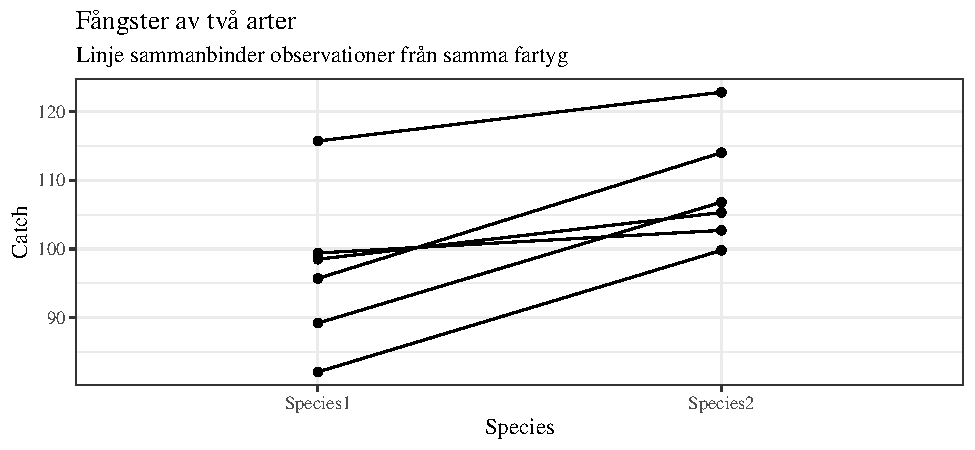
\includegraphics{R-anvisningar_files/figure-latex/unnamed-chunk-218-1} \end{center}

\begin{Shaded}
\begin{Highlighting}[]
\FunctionTok{ggplot}\NormalTok{(dat\_fish, }\FunctionTok{aes}\NormalTok{(Species1, Region)) }\SpecialCharTok{+} 
  \FunctionTok{geom\_point}\NormalTok{() }\SpecialCharTok{+}
  \FunctionTok{labs}\NormalTok{(}\AttributeTok{title =} \StringTok{"Fångster i två regioner"}\NormalTok{)}
\end{Highlighting}
\end{Shaded}

\begin{center}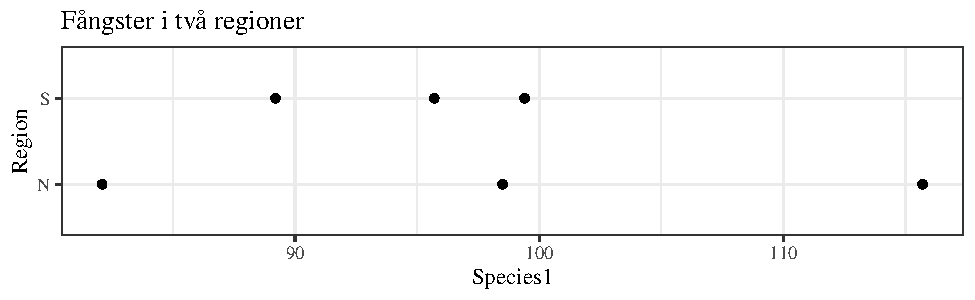
\includegraphics{R-anvisningar_files/figure-latex/unnamed-chunk-219-1} \end{center}

För arterna har vi matchad data - varje observation av den ena arten är kopplad till en observation från den andra arten eftersom den kommer från samma båt - och vi kan testa om medelfångsterna av de två arterna är lika med ett t-test. Hypoteserna ges av

\begin{itemize}
\tightlist
\item
  H0: populationsmedelvärdet av fångster för art 1 är lika med det för art 2,
\item
  H1: populationsmedelvärdena är ej lika.
\end{itemize}

I R kan ett test för matchad data genomföras med \texttt{t.test()} och argumentet \texttt{paired}, eller genom att beräkna differensen per båt och göra ett t-test för ett stickprov.

\begin{Shaded}
\begin{Highlighting}[]
\FunctionTok{t.test}\NormalTok{(dat\_fish}\SpecialCharTok{$}\NormalTok{Species1, dat\_fish}\SpecialCharTok{$}\NormalTok{Species2, }\AttributeTok{paired =}\NormalTok{ T)}
\end{Highlighting}
\end{Shaded}

\begin{verbatim}
## 
##  Paired t-test
## 
## data:  dat_fish$Species1 and dat_fish$Species2
## t = -4.2613, df = 5, p-value = 0.008005
## alternative hypothesis: true mean difference is not equal to 0
## 95 percent confidence interval:
##  -18.918238  -4.681762
## sample estimates:
## mean difference 
##           -11.8
\end{verbatim}

\begin{Shaded}
\begin{Highlighting}[]
\CommentTok{\# Alternativt}
\CommentTok{\# t.test(dat\_fish$Species1 {-} dat\_fish$Species2)}
\end{Highlighting}
\end{Shaded}

Det beräknade p-värdet ställs mot en signifikansnivå, vanligen fem procent, och om p-värdet är under signifikansnivån förkastar vi nollhypotesen. I det här exemplet tyder på värdet på att nollhypotesen inte stämmer - en art är vanligare än den andra.

För att jämföra regioner kan vi göra ett t-test för två oberoende stickprov. Hypoteser ges av

\begin{itemize}
\tightlist
\item
  H0: populationsmedelvärdet av fångster är lika mellan regioner,
\item
  H1: populationsmedelvärdet av fångster är ej lika mellan regioner.
\end{itemize}

Testet kan genomföras med \texttt{t.test()} och kan antingen göras med ett antagande om lika varianser (vilket motsvarar det som görs för hand under kursen) eller utan det antagandet. Variabler kan anges med en formel som \texttt{Species1\ \textasciitilde{}\ Group}, vilket vi kan tänka på som värden för art 1 uppdelat efter grupp.

\begin{Shaded}
\begin{Highlighting}[]
\FunctionTok{t.test}\NormalTok{(Species1 }\SpecialCharTok{\textasciitilde{}}\NormalTok{ Region, }\AttributeTok{data =}\NormalTok{ dat\_fish, }\AttributeTok{var.equal =}\NormalTok{ T)}
\end{Highlighting}
\end{Shaded}

\begin{verbatim}
## 
##  Two Sample t-test
## 
## data:  Species1 by Region
## t = 0.39416, df = 4, p-value = 0.7136
## alternative hypothesis: true difference in means between group N and group S is not equal to 0
## 95 percent confidence interval:
##  -24.17586  32.17586
## sample estimates:
## mean in group N mean in group S 
##        98.76667        94.76667
\end{verbatim}

Ett högt p-värde tyder på att det inte finns någon skillnad i fångst mellan regioner.

För data där utfallen är två eller flera kategorier kan ett chi-två-test testa om det finns något samband mellan två variabler. Följande data anger vilka partier ett urval väljare från tre kommuner planerar rösta på i nästa riksdagsval.

\begin{Shaded}
\begin{Highlighting}[]
\NormalTok{dat\_parti }\OtherTok{\textless{}{-}} \FunctionTok{data.frame}\NormalTok{(}\AttributeTok{Kommun =} \FunctionTok{c}\NormalTok{(}\StringTok{"Malmö"}\NormalTok{, }\StringTok{"Lund"}\NormalTok{, }\StringTok{"Kävlinge"}\NormalTok{),}
                        \AttributeTok{S =} \FunctionTok{c}\NormalTok{(}\DecValTok{54}\NormalTok{, }\DecValTok{102}\NormalTok{, }\DecValTok{40}\NormalTok{),}
                        \AttributeTok{M =} \FunctionTok{c}\NormalTok{(}\DecValTok{30}\NormalTok{, }\DecValTok{98}\NormalTok{, }\DecValTok{53}\NormalTok{),}
                        \AttributeTok{MP =} \FunctionTok{c}\NormalTok{(}\DecValTok{7}\NormalTok{, }\DecValTok{50}\NormalTok{, }\DecValTok{5}\NormalTok{))}
\NormalTok{dat\_parti}
\end{Highlighting}
\end{Shaded}

\begin{verbatim}
##     Kommun   S  M MP
## 1    Malmö  54 30  7
## 2     Lund 102 98 50
## 3 Kävlinge  40 53  5
\end{verbatim}

För att testa om det finns något samband mellan kommun och parti sätter vi upp hypoteserna

\begin{itemize}
\tightlist
\item
  H0: det finns inget samband mellan parti och kommun (ingen skillnad mellan kommuner),
\item
  H1: det finns något samband mellan parti och kommun.
\end{itemize}

Detta kan testas med ett chi-två-test med funktionen \texttt{chisq.test()}. Som argument ges den numeriska delen av korstabellen - vi tar alltså bort den första kolumnen för kommun.

\begin{Shaded}
\begin{Highlighting}[]
\FunctionTok{chisq.test}\NormalTok{(dat\_parti[, }\SpecialCharTok{{-}}\DecValTok{1}\NormalTok{])}
\end{Highlighting}
\end{Shaded}

\begin{verbatim}
## 
##  Pearson's Chi-squared test
## 
## data:  dat_parti[, -1]
## X-squared = 25.659, df = 4, p-value = 3.706e-05
\end{verbatim}

Det låga p-värdet på 0.000037 ger att vi förkastar nollhypotesen och drar slutsatsen att det finns ett samband mellan kommun och parti.

\section{Allmänt}\label{allmuxe4nt}

Variansanalys (eller \emph{anova-modellen}) är en statistisk modell där medelvärdet varierar beroende på en behandling och ett normalfördelat slumpfel. Från en anova-modell kan man beräkna ett F-test, som testar om det finns någon övergripande gruppskillnad, och post-hoc-test, som jämför specifika grupper med varandra.

Den specifika modellen beror på försöksupplägget. Här ges exempel på variansanalys med en faktor, en faktor med block, och två faktorer.

\section{Variansanalys. En faktor}\label{variansanalys.-en-faktor}

Vid variansanalys med en faktor har man observationer av en kontinuerlig utfallsvariabel från två eller flera behandlingsgrupper. Som exempel används en datamängd på ett odlingsförsök med tre behandlingar (varav en kontroll). Exemplet finns tillgängligt i R som \texttt{PlantGrowth}.

\begin{Shaded}
\begin{Highlighting}[]
\NormalTok{PlantGrowth}
\end{Highlighting}
\end{Shaded}

\begin{verbatim}
##    weight group
## 1    4.17  ctrl
## 2    5.58  ctrl
## 3    5.18  ctrl
## 4    6.11  ctrl
## 5    4.50  ctrl
## 6    4.61  ctrl
## 7    5.17  ctrl
## 8    4.53  ctrl
## 9    5.33  ctrl
## 10   5.14  ctrl
## 11   4.81  trt1
## 12   4.17  trt1
## 13   4.41  trt1
## 14   3.59  trt1
## 15   5.87  trt1
## 16   3.83  trt1
## 17   6.03  trt1
## 18   4.89  trt1
## 19   4.32  trt1
## 20   4.69  trt1
## 21   6.31  trt2
## 22   5.12  trt2
## 23   5.54  trt2
## 24   5.50  trt2
## 25   5.37  trt2
## 26   5.29  trt2
## 27   4.92  trt2
## 28   6.15  trt2
## 29   5.80  trt2
## 30   5.26  trt2
\end{verbatim}

Datan har 30 observationer av vikt \texttt{weight} och varje observation tillhör någon specifik behandling \texttt{group}. Datan kan illustreras med ett spridningsdiagram.

\begin{Shaded}
\begin{Highlighting}[]
\FunctionTok{ggplot}\NormalTok{(PlantGrowth, }\FunctionTok{aes}\NormalTok{(group, weight)) }\SpecialCharTok{+}
  \FunctionTok{geom\_point}\NormalTok{()}
\end{Highlighting}
\end{Shaded}

\begin{center}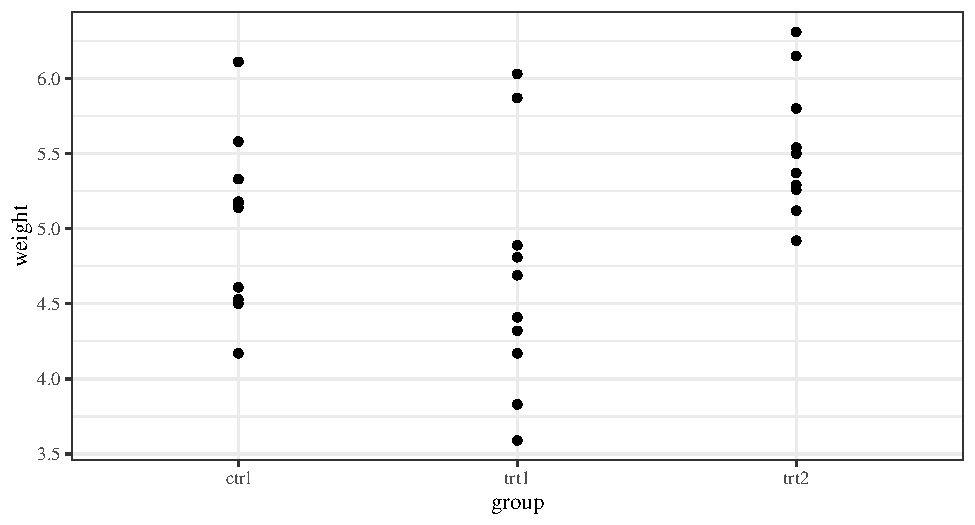
\includegraphics{R-anvisningar_files/figure-latex/unnamed-chunk-225-1} \end{center}

Behandling 1 verkar vara något lägre än kontrollen medan behandling 2 verkar vara något högre.

En anova-modell kan i R skattas med funktionen \texttt{lm()} (för \emph{linjär modell}). Från modellobjektet kan man sedan plocka fram en anova-tabell (som bland annat anger utfallet av F-testet) och genomföra parvisa jämförelser genom \texttt{emmeans}.

\begin{Shaded}
\begin{Highlighting}[]
\NormalTok{mod }\OtherTok{\textless{}{-}} \FunctionTok{lm}\NormalTok{(weight }\SpecialCharTok{\textasciitilde{}}\NormalTok{ group, }\AttributeTok{data =}\NormalTok{ PlantGrowth)}
\end{Highlighting}
\end{Shaded}

Modellen anges som en formel \texttt{weight\ \textasciitilde{}\ group}, vilket kan utläsas \emph{vikt beroende på behandlingsgrupp}. Därefter anges data med argumentet \texttt{data}.

För anova-tabellen finns flera alternativ. Här används funktionen \texttt{Anova()} från paketet \texttt{car}.

\begin{Shaded}
\begin{Highlighting}[]
\FunctionTok{library}\NormalTok{(car)}
\FunctionTok{Anova}\NormalTok{(mod)}
\end{Highlighting}
\end{Shaded}

\begin{verbatim}
## Anova Table (Type II tests)
## 
## Response: weight
##            Sum Sq Df F value  Pr(>F)  
## group      3.7663  2  4.8461 0.01591 *
## Residuals 10.4921 27                  
## ---
## Signif. codes:  0 '***' 0.001 '**' 0.01 '*' 0.05 '.' 0.1 ' ' 1
\end{verbatim}

Anova-tabellen ger kvadratsummor (\texttt{Sum\ Sq}), frihetsgrader (\texttt{Df}) och utfallet av ett F-test. Testets hypoteser ges av

H0: alla behandlingsgrupper har samma medelvärde
H1: alla behandlingsgrupper har inte samma medelvärde

Det låga p-värdet tyder på att nollhypotesen bör förkastas, vilket alltså pekar på att det finns någon eller några skillnader i medelvärde.

\begin{exercise}[Anova för hand]
Anovatabell från \texttt{Anova()} ger kvadratsummor och frihetsgrader. Använd den informationen för att, för hand, beräkna medelkvadratsummor och F-värdet.
\end{exercise}

\begin{exercise}[Tabellvärde för F-fördelningen]

Anova-tabellen ger ett p-värde från vilket vi kan dra en direkt slutsats. Om man istället löser uppgiften för hand ställer man det beräknade F-värdet mot ett kritiskt värde från en tabell över F-fördelningen. Se efter om man kan hitta ett lämpligt tabellvärde för det aktuella testet (med 2 och 27 frihetsgrader). Det är möjligt att det inte finns en rad för 27 i en vanlig F-fördelningstabell, använd isåfall värdet på närmast övre rad (t.ex. 26 eller 25). I R kan kvantiler för F-fördelningen tas fram med \texttt{qf()}, t.ex.

\begin{Shaded}
\begin{Highlighting}[]
\FunctionTok{qf}\NormalTok{(}\FloatTok{0.95}\NormalTok{, }\DecValTok{2}\NormalTok{, }\DecValTok{27}\NormalTok{)}
\end{Highlighting}
\end{Shaded}

\begin{verbatim}
## [1] 3.354131
\end{verbatim}

\end{exercise}

En naturlig följdfråga är vilka behandlingsgrupper som skiljer sig åt. För att besvara det krävs \emph{parvisa jämförelser} där behandlingarna jämförs två och två. Parvisa jämförelse kan göras med paketet \texttt{emmeans} och funktionen med samma namn. Funktionen tar modellobjektet som första argument och en formel för jämförelsetyp som andra argument (här \texttt{pairwise\ \textasciitilde{}\ group}, en parvis jämförelse mellan nivåer i \texttt{group}).

\begin{Shaded}
\begin{Highlighting}[]
\CommentTok{\# install.packages("emmeans")}
\FunctionTok{library}\NormalTok{(emmeans)}
\FunctionTok{emmeans}\NormalTok{(mod, pairwise }\SpecialCharTok{\textasciitilde{}}\NormalTok{ group)}
\end{Highlighting}
\end{Shaded}

\begin{verbatim}
## $emmeans
##  group emmean    SE df lower.CL upper.CL
##  ctrl    5.03 0.197 27     4.63     5.44
##  trt1    4.66 0.197 27     4.26     5.07
##  trt2    5.53 0.197 27     5.12     5.93
## 
## Confidence level used: 0.95 
## 
## $contrasts
##  contrast    estimate    SE df t.ratio p.value
##  ctrl - trt1    0.371 0.279 27   1.331  0.3909
##  ctrl - trt2   -0.494 0.279 27  -1.772  0.1980
##  trt1 - trt2   -0.865 0.279 27  -3.103  0.0120
## 
## P value adjustment: tukey method for comparing a family of 3 estimates
\end{verbatim}

I den nedre tabellen med jämförelser ges alla parvisa jämförelser. Nollhypotesen är att de två grupper som jämförs har samma medelvärde - ett lågt p-värde tyder alltså på att de två grupperna är signifikant skilda. Notera också att p-värden justeras med tukey-metoden, även känt som Tukeys HSD.

Om man istället vill använda Fishers LSD kan man styra justeringen med argumentet \texttt{adjust}.

\begin{Shaded}
\begin{Highlighting}[]
\FunctionTok{emmeans}\NormalTok{(mod, pairwise }\SpecialCharTok{\textasciitilde{}}\NormalTok{ group, }\AttributeTok{adjust =} \StringTok{"none"}\NormalTok{)}
\end{Highlighting}
\end{Shaded}

\begin{verbatim}
## $emmeans
##  group emmean    SE df lower.CL upper.CL
##  ctrl    5.03 0.197 27     4.63     5.44
##  trt1    4.66 0.197 27     4.26     5.07
##  trt2    5.53 0.197 27     5.12     5.93
## 
## Confidence level used: 0.95 
## 
## $contrasts
##  contrast    estimate    SE df t.ratio p.value
##  ctrl - trt1    0.371 0.279 27   1.331  0.1944
##  ctrl - trt2   -0.494 0.279 27  -1.772  0.0877
##  trt1 - trt2   -0.865 0.279 27  -3.103  0.0045
\end{verbatim}

Parvisa jämförelser presenteras ofta med signifikansbokstäver (en. \emph{compact letter display, cld}). Dessa kan plockas fram med \texttt{multcomp}-paketet och funktionen \texttt{cld()}.

\begin{Shaded}
\begin{Highlighting}[]
\NormalTok{em }\OtherTok{\textless{}{-}} \FunctionTok{emmeans}\NormalTok{(mod, pairwise }\SpecialCharTok{\textasciitilde{}}\NormalTok{ group)}

\FunctionTok{library}\NormalTok{(multcomp)}
\FunctionTok{cld}\NormalTok{(em, }\AttributeTok{Letters =}\NormalTok{ letters)}
\end{Highlighting}
\end{Shaded}

\begin{verbatim}
##  group emmean    SE df lower.CL upper.CL .group
##  trt1    4.66 0.197 27     4.26     5.07  a    
##  ctrl    5.03 0.197 27     4.63     5.44  ab   
##  trt2    5.53 0.197 27     5.12     5.93   b   
## 
## Confidence level used: 0.95 
## P value adjustment: tukey method for comparing a family of 3 estimates 
## significance level used: alpha = 0.05 
## NOTE: If two or more means share the same grouping symbol,
##       then we cannot show them to be different.
##       But we also did not show them to be the same.
\end{verbatim}

Tolkning av grupperingen till höger är att grupper som delar en bokstav inte är signifikant skilda. I det här fallet är den lägsta nivån skild från de två högsta. I övrigt finns inga signifikanta skillnader. Jämför gärna med p-värdena från tabellen med parvisa jämförelser. Man bör se att parvisa jämförelser med ett p-värde under fem procent motsvaras av att de behandlingarna inte delar någon bokstav i bokstavstabellen.

\begin{exercise}[Anova med två behandlingar]

Följande kod skapar en datamängd med två behandlingar.

\begin{Shaded}
\begin{Highlighting}[]
\NormalTok{dat\_two }\OtherTok{\textless{}{-}}\NormalTok{ PlantGrowth }\SpecialCharTok{\%\textgreater{}\%} \FunctionTok{filter}\NormalTok{(group }\SpecialCharTok{\%in\%} \FunctionTok{c}\NormalTok{(}\StringTok{"trt1"}\NormalTok{, }\StringTok{"trt2"}\NormalTok{))}
\end{Highlighting}
\end{Shaded}

Använd den datan för att göra ett t-test för två oberoende stickprov med lika varians, ett t-test för två oberoende stickprov utan antagande om lika varians, och ett F-test (ofullständig exempelkod nedan). Vad kan sägas om p-värdena från de tre testen?

\begin{Shaded}
\begin{Highlighting}[]
\FunctionTok{t.test}\NormalTok{(\_\_\_ }\SpecialCharTok{\textasciitilde{}}\NormalTok{ group, }\AttributeTok{data =}\NormalTok{ dat\_two, }\AttributeTok{var.equal =}\NormalTok{ T)}
\FunctionTok{t.test}\NormalTok{(weight }\SpecialCharTok{\textasciitilde{}}\NormalTok{ \_\_\_, }\AttributeTok{data =}\NormalTok{ dat\_two, }\AttributeTok{var.equal =}\NormalTok{ F)}

\NormalTok{mod }\OtherTok{\textless{}{-}} \FunctionTok{lm}\NormalTok{(weight }\SpecialCharTok{\textasciitilde{}}\NormalTok{ group, }\AttributeTok{data =}\NormalTok{ \_\_\_)}
\FunctionTok{Anova}\NormalTok{(mod)}
\end{Highlighting}
\end{Shaded}

\end{exercise}

\begin{exercise}[Mass-signifikans]
Anledning till att vi justerar p-värden är att man vid varje test har en sannolikhet att förkasta. Om man gör ett stort antal tester är man nästan garanterad att få något (falskt) signifikant resultat. Justering höjer p-värdena för att minska den risken. Följande kod simulerar data med 5 grupper och producerar de parvisa jämförelserna.

\begin{Shaded}
\begin{Highlighting}[]
\NormalTok{n\_groups }\OtherTok{\textless{}{-}} \DecValTok{5}
\NormalTok{dat\_sim }\OtherTok{\textless{}{-}} \FunctionTok{expand\_grid}\NormalTok{(}\AttributeTok{obs =} \DecValTok{1}\SpecialCharTok{:}\DecValTok{10}\NormalTok{, }\AttributeTok{group =}\NormalTok{ letters[}\DecValTok{1}\SpecialCharTok{:}\NormalTok{n\_groups]) }\SpecialCharTok{\%\textgreater{}\%} \FunctionTok{mutate}\NormalTok{(}\AttributeTok{y =} \FunctionTok{rnorm}\NormalTok{(}\FunctionTok{n}\NormalTok{()))}
\NormalTok{mod }\OtherTok{\textless{}{-}} \FunctionTok{lm}\NormalTok{(y }\SpecialCharTok{\textasciitilde{}}\NormalTok{ group, dat\_sim)}
\FunctionTok{emmeans}\NormalTok{(mod, pairwise }\SpecialCharTok{\textasciitilde{}}\NormalTok{ group, }\AttributeTok{adjust =} \StringTok{"none"}\NormalTok{)}
\end{Highlighting}
\end{Shaded}

\begin{verbatim}
## $emmeans
##  group  emmean    SE df lower.CL upper.CL
##  a      0.3102 0.344 45   -0.382    1.003
##  b      0.1899 0.344 45   -0.503    0.882
##  c     -0.2747 0.344 45   -0.967    0.418
##  d     -0.3239 0.344 45   -1.016    0.369
##  e      0.0984 0.344 45   -0.594    0.791
## 
## Confidence level used: 0.95 
## 
## $contrasts
##  contrast estimate    SE df t.ratio p.value
##  a - b      0.1204 0.486 45   0.248  0.8056
##  a - c      0.5849 0.486 45   1.203  0.2352
##  a - d      0.6341 0.486 45   1.304  0.1988
##  a - e      0.2119 0.486 45   0.436  0.6651
##  b - c      0.4645 0.486 45   0.956  0.3444
##  b - d      0.5137 0.486 45   1.057  0.2963
##  b - e      0.0915 0.486 45   0.188  0.8515
##  c - d      0.0492 0.486 45   0.101  0.9198
##  c - e     -0.3730 0.486 45  -0.767  0.4469
##  d - e     -0.4222 0.486 45  -0.868  0.3897
\end{verbatim}

Kör koden tio gånger. Hur många gånger av de tio ger de parvisa jämförelserna \emph{någon} signifikant skillnad (det vill säga något p-värde under 0.05)?

En passande xkcd-serie: \url{https://xkcd.com/882/}
\end{exercise}

\begin{exercise}[Äppelinfektionsimport]
En studie har givit ett mått på infektion hos äppelträd. Fyra sorter jämförs med tre replikat per sort. Data finns i fliken \emph{Äppelangrepp} i excelfilen \emph{Uppgiftsdata.xslx} på canvassidan. Fyll i kodstycket nedan för att importera datan.
\end{exercise}

\begin{exercise}[Äppelinfektionsgraf]

Fyll i kodstycket nedan för att skapa en graf av äppeldatan.

\begin{Shaded}
\begin{Highlighting}[]
\FunctionTok{ggplot}\NormalTok{(\_\_\_, }\FunctionTok{aes}\NormalTok{(}\AttributeTok{x =}\NormalTok{ \_\_\_, }\AttributeTok{y =}\NormalTok{ \_\_\_)) }\SpecialCharTok{+}
  \FunctionTok{geom\_point}\NormalTok{()}
\end{Highlighting}
\end{Shaded}

\end{exercise}

\begin{exercise}[Äppelinfektionsmodell]

Fyll i kodstycket nedan för att skatta en anovamodell och ta fram anovatabellen. Vad är F-testets noll- och alternativhypotes? Vilken slutsats kan man dra från testet?

\begin{Shaded}
\begin{Highlighting}[]
\NormalTok{mod }\OtherTok{\textless{}{-}} \FunctionTok{lm}\NormalTok{(\_\_\_ }\SpecialCharTok{\textasciitilde{}}\NormalTok{ \_\_\_, }\AttributeTok{data =}\NormalTok{ dat\_apple)}
\FunctionTok{Anova}\NormalTok{(mod)}
\end{Highlighting}
\end{Shaded}

\end{exercise}

\section{Variansanalys. En faktor med block}\label{variansanalys.-en-faktor-med-block}

I en blockdesign delas försöksobjekten (de enheter man ger en behandling och sedan mäter, t.ex. en försöksruta eller en planta) in i grupper av lika objekt (ett \emph{block}). Sedan ger man enheterna inom blocket varsin behandling. Blockförsök är ofta balanserade, så att varje behandling förekommer en gång i varje block.

Som exempel på ett blockförsök kan vi titta på datan \texttt{oats} från paketet \texttt{MASS}. Datan kommer från ett agrikulturellt försök och blockdesignen sker genom att man delar in ett fält i flera delar (blocken) och sätter varje behandling i varje block. Datan har två faktorer (kväve \texttt{N} och sort \texttt{V}), men låt oss i den här första delen titta på en specifik sort.

\begin{Shaded}
\begin{Highlighting}[]
\FunctionTok{library}\NormalTok{(MASS)}
\NormalTok{oats\_marvel }\OtherTok{\textless{}{-}}\NormalTok{ oats }\SpecialCharTok{\%\textgreater{}\%} \FunctionTok{filter}\NormalTok{(V }\SpecialCharTok{==} \StringTok{"Marvellous"}\NormalTok{)}
\NormalTok{oats\_marvel}
\end{Highlighting}
\end{Shaded}

\begin{verbatim}
##      B          V      N   Y
## 1    I Marvellous 0.0cwt 105
## 2    I Marvellous 0.2cwt 140
## 3    I Marvellous 0.4cwt 118
## 4    I Marvellous 0.6cwt 156
## 5   II Marvellous 0.0cwt  96
## 6   II Marvellous 0.2cwt 124
## 7   II Marvellous 0.4cwt 121
## 8   II Marvellous 0.6cwt 144
## 9  III Marvellous 0.0cwt  89
## 10 III Marvellous 0.2cwt 129
## 11 III Marvellous 0.4cwt 132
## 12 III Marvellous 0.6cwt 124
## 13  IV Marvellous 0.0cwt  70
## 14  IV Marvellous 0.2cwt  89
## 15  IV Marvellous 0.4cwt 104
## 16  IV Marvellous 0.6cwt 117
## 17   V Marvellous 0.0cwt  63
## 18   V Marvellous 0.2cwt  70
## 19   V Marvellous 0.4cwt 109
## 20   V Marvellous 0.6cwt  99
## 21  VI Marvellous 0.0cwt  97
## 22  VI Marvellous 0.2cwt  99
## 23  VI Marvellous 0.4cwt 119
## 24  VI Marvellous 0.6cwt 121
\end{verbatim}

En vanlig illustration av ett blockförsök är ett punktdiagram kombinerat med ett linjediagram.

\begin{Shaded}
\begin{Highlighting}[]
\FunctionTok{ggplot}\NormalTok{(oats\_marvel, }\FunctionTok{aes}\NormalTok{(N, Y, }\AttributeTok{color =}\NormalTok{ B, }\AttributeTok{group =}\NormalTok{ B)) }\SpecialCharTok{+}
  \FunctionTok{geom\_point}\NormalTok{(}\AttributeTok{size =} \DecValTok{4}\NormalTok{) }\SpecialCharTok{+}
  \FunctionTok{geom\_line}\NormalTok{()}
\end{Highlighting}
\end{Shaded}

\begin{center}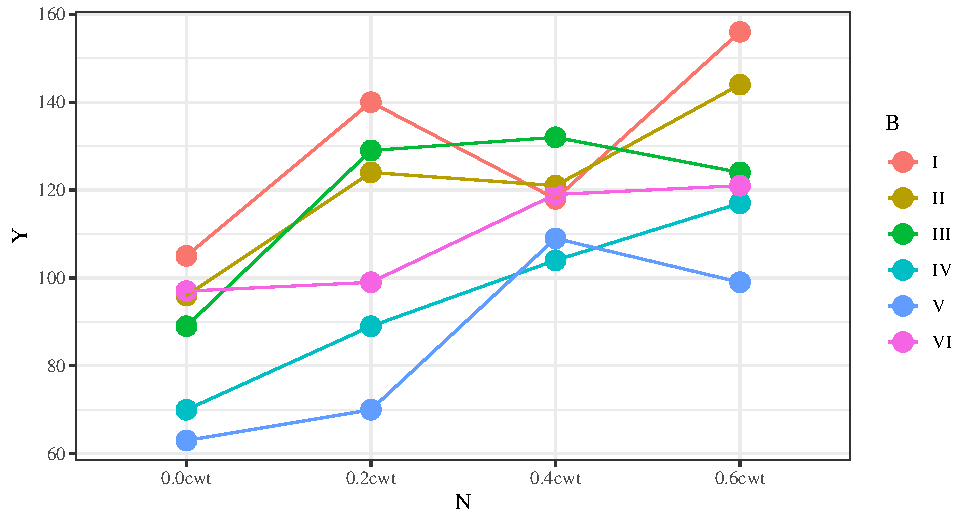
\includegraphics{R-anvisningar_files/figure-latex/unnamed-chunk-239-1} \end{center}

Färg och linje sammanbinder observationer från samma block. Det finns tecken på en blockeffekt: block I är nästan alltid högst och block V är nästan alltid lägst. Det finns också en tydlig behandlingseffekt i att högre kväve ger högre skörd.

Blockeffekten kan enkelt föras in i modellen genom att lägga till variabeln \texttt{B} i \texttt{lm}-funktionen. Anova-tabellen och parvisa jämförelser kan göras på samma sätt som tidigare. Resultaten påverkas av att modellen har en blockfaktor; man behöver vanligen inte ange det explicit.

\begin{Shaded}
\begin{Highlighting}[]
\NormalTok{mod\_bl }\OtherTok{\textless{}{-}} \FunctionTok{lm}\NormalTok{(Y }\SpecialCharTok{\textasciitilde{}}\NormalTok{ N }\SpecialCharTok{+}\NormalTok{ B, }\AttributeTok{data =}\NormalTok{ oats\_marvel)}
\FunctionTok{Anova}\NormalTok{(mod\_bl)}
\end{Highlighting}
\end{Shaded}

\begin{verbatim}
## Anova Table (Type II tests)
## 
## Response: Y
##           Sum Sq Df F value    Pr(>F)    
## N         5287.5  3 14.6241 0.0001004 ***
## B         5708.7  5  9.4735 0.0003106 ***
## Residuals 1807.8 15                      
## ---
## Signif. codes:  0 '***' 0.001 '**' 0.01 '*' 0.05 '.' 0.1 ' ' 1
\end{verbatim}

P-värdet från F-testet på variabeln N är nu klart mindre än tidigare. Detta beror på att en stor del av variationen kan förklaras med blockeffekten, vilket är tydligt i att blockeffekten också har ett litet p-värde i F-testet.

Det kan vara intressant att jämföra med modellen utan block.

\begin{Shaded}
\begin{Highlighting}[]
\NormalTok{mod\_wo\_block }\OtherTok{\textless{}{-}} \FunctionTok{lm}\NormalTok{(Y }\SpecialCharTok{\textasciitilde{}}\NormalTok{ N, }\AttributeTok{data =}\NormalTok{ oats\_marvel)}
\FunctionTok{Anova}\NormalTok{(mod\_wo\_block)}
\end{Highlighting}
\end{Shaded}

\begin{verbatim}
## Anova Table (Type II tests)
## 
## Response: Y
##           Sum Sq Df F value  Pr(>F)  
## N         5287.5  3  4.6896 0.01227 *
## Residuals 7516.5 20                  
## ---
## Signif. codes:  0 '***' 0.001 '**' 0.01 '*' 0.05 '.' 0.1 ' ' 1
\end{verbatim}

Det som är residualens kvadratsumma i modellen utan block är i blockmodellen uppdelat i en blockeffekt och en residualterm. Eftersom F-testet bygger på en jämförelse mellan behandlingseffekten och residualtermen leder blockdesignen till starkare signifikans i blockmodellen. Å andra sidan kostar blockfaktorn frihetsgrader vilket ger oss ett svagare test. Effekten av att ta med ett block beror alltså på om det finns en verklig skillnad mellan blocken eller ej.

Vi kan gå vidare med att titta på parvisa jämförelser mellan kvävenivåer. Funktionen \texttt{emmeans()} och \texttt{cld()} fungerar som tidigare.

\begin{Shaded}
\begin{Highlighting}[]
\FunctionTok{cld}\NormalTok{(}\FunctionTok{emmeans}\NormalTok{(mod\_bl, }\SpecialCharTok{\textasciitilde{}}\NormalTok{ N), }\AttributeTok{Letters =}\NormalTok{ letters)}
\end{Highlighting}
\end{Shaded}

\begin{verbatim}
##  N      emmean   SE df lower.CL upper.CL .group
##  0.0cwt   86.7 4.48 15     77.1     96.2  a    
##  0.2cwt  108.5 4.48 15     98.9    118.1   b   
##  0.4cwt  117.2 4.48 15    107.6    126.7   bc  
##  0.6cwt  126.8 4.48 15    117.3    136.4    c  
## 
## Results are averaged over the levels of: B 
## Confidence level used: 0.95 
## P value adjustment: tukey method for comparing a family of 4 estimates 
## significance level used: alpha = 0.05 
## NOTE: If two or more means share the same grouping symbol,
##       then we cannot show them to be different.
##       But we also did not show them to be the same.
\end{verbatim}

Signifikansbokstäver anger att den lägsta nivån är skild från övriga och att den näst lägsta är skild från den högsta. Även här kan det vara intressant att jämföra med modellen utan block.

\begin{Shaded}
\begin{Highlighting}[]
\FunctionTok{cld}\NormalTok{(}\FunctionTok{emmeans}\NormalTok{(mod\_wo\_block, }\SpecialCharTok{\textasciitilde{}}\NormalTok{ N), }\AttributeTok{Letters =}\NormalTok{ letters)}
\end{Highlighting}
\end{Shaded}

\begin{verbatim}
##  N      emmean   SE df lower.CL upper.CL .group
##  0.0cwt   86.7 7.91 20     70.2      103  a    
##  0.2cwt  108.5 7.91 20     92.0      125  ab   
##  0.4cwt  117.2 7.91 20    100.7      134  ab   
##  0.6cwt  126.8 7.91 20    110.3      143   b   
## 
## Confidence level used: 0.95 
## P value adjustment: tukey method for comparing a family of 4 estimates 
## significance level used: alpha = 0.05 
## NOTE: If two or more means share the same grouping symbol,
##       then we cannot show them to be different.
##       But we also did not show them to be the same.
\end{verbatim}

Modellen utan block ger samma medelvärden \texttt{emmean} men större medelfel \texttt{SE} och färre signifikanta skillnader.

\begin{exercise}[Block med två behandlingar. Graf]

Det minsta möjliga blocket är det med två behandlingar. Vi filtrerar havredatan för att den situationen.

\begin{Shaded}
\begin{Highlighting}[]
\NormalTok{dat\_small\_block }\OtherTok{\textless{}{-}}\NormalTok{ oats }\SpecialCharTok{\%\textgreater{}\%} \FunctionTok{filter}\NormalTok{(V }\SpecialCharTok{==} \StringTok{"Marvellous"}\NormalTok{, N }\SpecialCharTok{\%in\%} \FunctionTok{c}\NormalTok{(}\StringTok{"0.6cwt"}\NormalTok{, }\StringTok{"0.0cwt"}\NormalTok{))}
\NormalTok{dat\_small\_block}
\end{Highlighting}
\end{Shaded}

\begin{verbatim}
##      B          V      N   Y
## 1    I Marvellous 0.0cwt 105
## 2    I Marvellous 0.6cwt 156
## 3   II Marvellous 0.0cwt  96
## 4   II Marvellous 0.6cwt 144
## 5  III Marvellous 0.0cwt  89
## 6  III Marvellous 0.6cwt 124
## 7   IV Marvellous 0.0cwt  70
## 8   IV Marvellous 0.6cwt 117
## 9    V Marvellous 0.0cwt  63
## 10   V Marvellous 0.6cwt  99
## 11  VI Marvellous 0.0cwt  97
## 12  VI Marvellous 0.6cwt 121
\end{verbatim}

Fyll i stycket nedan för att skapa en graf med \texttt{N} på x-axeln, \texttt{Y} på y-axeln och en gruppering som länkar observationer från samma block.

\begin{Shaded}
\begin{Highlighting}[]
\FunctionTok{ggplot}\NormalTok{(dat\_small\_block, }\FunctionTok{aes}\NormalTok{(}\AttributeTok{x =}\NormalTok{ \_\_\_, }\AttributeTok{y =}\NormalTok{ \_\_\_, }\AttributeTok{group =}\NormalTok{ \_\_\_)) }\SpecialCharTok{+}
  \FunctionTok{geom\_point}\NormalTok{() }\SpecialCharTok{+}
  \FunctionTok{geom\_line}\NormalTok{()}
\end{Highlighting}
\end{Shaded}

\end{exercise}

\begin{exercise}[Block med två behandlingar. Test]

Eftersom det är ett försök med en förklarande faktor och block kan man modellera det med den tidigare blockmodellen. Men eftersom man bara har två observationer per block kan man också se det som matchade stickprov, vilket kan lösas med ett t-test. Fyll i stycket nedan för att göra de två testen - utfallsvariabeln är skörd \texttt{Y} och den förklarande faktorn är kvävenivån \texttt{N}. Jämför resultaten.

\begin{Shaded}
\begin{Highlighting}[]
\NormalTok{mod }\OtherTok{\textless{}{-}} \FunctionTok{lm}\NormalTok{(\_\_\_ }\SpecialCharTok{\textasciitilde{}}\NormalTok{ \_\_\_ }\SpecialCharTok{+}\NormalTok{ B, }\AttributeTok{data =}\NormalTok{ dat\_small\_block)}
\FunctionTok{Anova}\NormalTok{(mod)}

\FunctionTok{t.test}\NormalTok{(\_\_\_ }\SpecialCharTok{\textasciitilde{}}\NormalTok{ \_\_\_, }\AttributeTok{data =}\NormalTok{ dat\_small\_block, }\AttributeTok{paired =}\NormalTok{ \_\_\_)}
\end{Highlighting}
\end{Shaded}

\end{exercise}

\begin{exercise}[Majshybridimport]

I fliken \emph{Majshybrider} i excelfilen \emph{Uppgiftsdata.xlsx} finns data på fyra majssorter, vardera sorterad på fem platser (som agerar som block). Importera datan med funktionen \texttt{read\_excel()} genom att fylla i kodstycket nedan.

\begin{Shaded}
\begin{Highlighting}[]
\NormalTok{dat\_corn }\OtherTok{\textless{}{-}} \FunctionTok{read\_excel}\NormalTok{(}\StringTok{""}\NormalTok{, }\AttributeTok{sheet =}\NormalTok{ \_\_\_)}
\end{Highlighting}
\end{Shaded}

\end{exercise}

\begin{exercise}[Majshybridgraf]
Skapa en lämplig graf av datan på majshybrider. Grafen ska illustrera både jämförelsen mellan hybrider och jämförelsen mellan platser. Se exemplet ovan som guide.
\end{exercise}

\begin{exercise}[Majshybridmodell]

Fyll i koden nedan för att skatta en anova-modell med block för datan på majshybrider. Ta fram anovatabellen med \texttt{Anova()}. Vilka slutsatser kan man dra från anovatabellen?

\begin{Shaded}
\begin{Highlighting}[]
\NormalTok{mod }\OtherTok{\textless{}{-}} \FunctionTok{lm}\NormalTok{(\_\_\_ }\SpecialCharTok{\textasciitilde{}}\NormalTok{ \_\_\_ }\SpecialCharTok{+}\NormalTok{ Plats, }\AttributeTok{data =}\NormalTok{ dat\_corn)}
\FunctionTok{Anova}\NormalTok{(mod)}
\end{Highlighting}
\end{Shaded}

\end{exercise}

\begin{exercise}[Majshybridjämförelser]

Gör lämplig ändring i koden nedan för att jämföra hybrider, istället för platser.

\begin{Shaded}
\begin{Highlighting}[]
\FunctionTok{emmeans}\NormalTok{(mod, pairwise }\SpecialCharTok{\textasciitilde{}}\NormalTok{ Plats)}
\end{Highlighting}
\end{Shaded}

\end{exercise}

\section{Variansanalys. Två faktorer med block}\label{variansanalys.-tvuxe5-faktorer-med-block}

Exempeldata på havre tar med två förklarande faktorer och ett block. Datan kan illustreras med ett punktdiagram där \texttt{facet\_wrap} delar grafen efter sort.

\begin{Shaded}
\begin{Highlighting}[]
\FunctionTok{ggplot}\NormalTok{(oats, }\FunctionTok{aes}\NormalTok{(N, Y, }\AttributeTok{color =}\NormalTok{ B)) }\SpecialCharTok{+}
  \FunctionTok{geom\_point}\NormalTok{(}\AttributeTok{size =} \DecValTok{4}\NormalTok{) }\SpecialCharTok{+}
  \FunctionTok{facet\_wrap}\NormalTok{(}\SpecialCharTok{\textasciitilde{}}\NormalTok{ V)}
\end{Highlighting}
\end{Shaded}

\begin{center}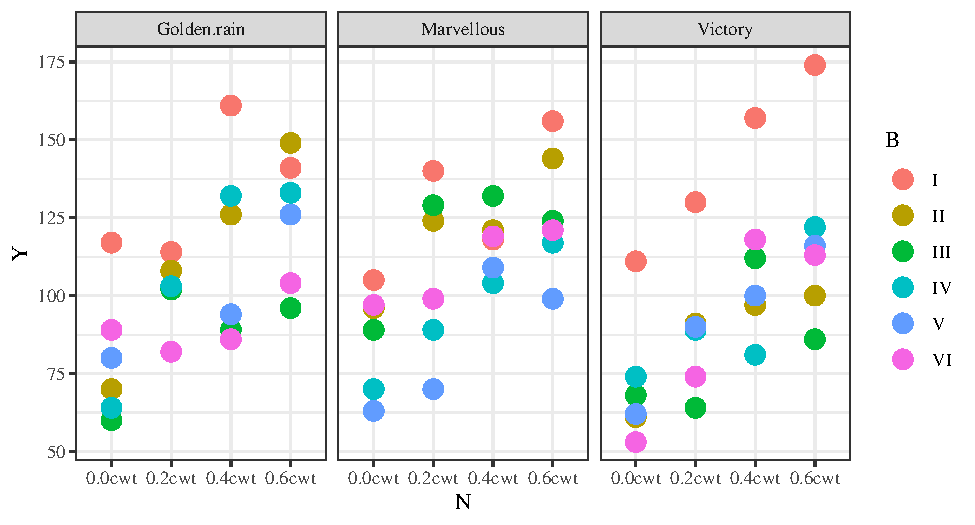
\includegraphics{R-anvisningar_files/figure-latex/unnamed-chunk-250-1} \end{center}

Grafen visar samma kvävesamband som tidigare. Det finns inga tydliga skillnader mellan sorter, möjligen har sorten Victory givit något lägre skörd än övriga. Det finns fortfarande en tydlig blockeffekt, till exempel har block I höga värden och block V låga värden.

Modellen skattas genom att lägga till variabeln för sort (V för variety) i \texttt{lm}-formeln. En modell med två faktorer kan antingen vara med eller utan en \emph{interaktion}. Interaktionstermen fångar påverkan mellan faktorerna. Ett exempel hade varit om någon sort svarat starkare på ökad kväve än någon annan. Standardmodellen är att ta med interaktionen, vilket vi anger genom att sätta \texttt{N\ *\ V} istället för \texttt{N\ +\ V}. Blocket tas fortfarande med som en adderad faktor

\begin{Shaded}
\begin{Highlighting}[]
\NormalTok{mod\_two\_fact }\OtherTok{\textless{}{-}} \FunctionTok{lm}\NormalTok{(Y }\SpecialCharTok{\textasciitilde{}}\NormalTok{ N }\SpecialCharTok{*}\NormalTok{ V }\SpecialCharTok{+}\NormalTok{ B, }\AttributeTok{data =}\NormalTok{ oats)}
\end{Highlighting}
\end{Shaded}

Anovatabellen kan plockas fram på samma sätt som tidigare.

\begin{Shaded}
\begin{Highlighting}[]
\FunctionTok{Anova}\NormalTok{(mod\_two\_fact)}
\end{Highlighting}
\end{Shaded}

\begin{verbatim}
## Anova Table (Type II tests)
## 
## Response: Y
##            Sum Sq Df F value    Pr(>F)    
## N         20020.5  3 26.2510 1.135e-10 ***
## V          1786.4  2  3.5134   0.03665 *  
## B         15875.3  5 12.4894 4.093e-08 ***
## N:V         321.7  6  0.2109   0.97187    
## Residuals 13982.1 55                      
## ---
## Signif. codes:  0 '***' 0.001 '**' 0.01 '*' 0.05 '.' 0.1 ' ' 1
\end{verbatim}

Raden \texttt{N:V} gäller interaktionseffekten mellan kväve och sort. I det här fallet är det ingen signifikant interaktion - vilket tyder på att sorterna svarar på kvävebehandling på liknande sätt. Samtliga huvudeffekter (raderna för N, V och B) är signifikanta. Kvadratsummorna och p-värdena tyder på att kväve förklarar mer av variationen än sort, vilket också är i linje med grafen ovan.

Vid flerfaktoriella försök kan man presentera parvisa jämförelser på flera olika sätt. Man kan ange huvudeffekter för en faktor utan att ange den andra faktorn, man kan ange medelvärden för samtliga kombinationer av två faktorer, och man kan ange medelvärden uppdelat efter nivåer i en annan faktor.

\begin{Shaded}
\begin{Highlighting}[]
\FunctionTok{emmeans}\NormalTok{(mod\_two\_fact, }\SpecialCharTok{\textasciitilde{}}\NormalTok{ N)}
\end{Highlighting}
\end{Shaded}

\begin{verbatim}
##  N      emmean   SE df lower.CL upper.CL
##  0.0cwt   79.4 3.76 55     71.9     86.9
##  0.2cwt   98.9 3.76 55     91.4    106.4
##  0.4cwt  114.2 3.76 55    106.7    121.8
##  0.6cwt  123.4 3.76 55    115.9    130.9
## 
## Results are averaged over the levels of: V, B 
## Confidence level used: 0.95
\end{verbatim}

\begin{Shaded}
\begin{Highlighting}[]
\FunctionTok{emmeans}\NormalTok{(mod\_two\_fact, }\SpecialCharTok{\textasciitilde{}}\NormalTok{ N }\SpecialCharTok{+}\NormalTok{ V)}
\end{Highlighting}
\end{Shaded}

\begin{verbatim}
##  N      V           emmean   SE df lower.CL upper.CL
##  0.0cwt Golden.rain   80.0 6.51 55     67.0     93.0
##  0.2cwt Golden.rain   98.5 6.51 55     85.5    111.5
##  0.4cwt Golden.rain  114.7 6.51 55    101.6    127.7
##  0.6cwt Golden.rain  124.8 6.51 55    111.8    137.9
##  0.0cwt Marvellous    86.7 6.51 55     73.6     99.7
##  0.2cwt Marvellous   108.5 6.51 55     95.5    121.5
##  0.4cwt Marvellous   117.2 6.51 55    104.1    130.2
##  0.6cwt Marvellous   126.8 6.51 55    113.8    139.9
##  0.0cwt Victory       71.5 6.51 55     58.5     84.5
##  0.2cwt Victory       89.7 6.51 55     76.6    102.7
##  0.4cwt Victory      110.8 6.51 55     97.8    123.9
##  0.6cwt Victory      118.5 6.51 55    105.5    131.5
## 
## Results are averaged over the levels of: B 
## Confidence level used: 0.95
\end{verbatim}

\begin{Shaded}
\begin{Highlighting}[]
\FunctionTok{emmeans}\NormalTok{(mod\_two\_fact, }\SpecialCharTok{\textasciitilde{}}\NormalTok{ N }\SpecialCharTok{|}\NormalTok{ V)}
\end{Highlighting}
\end{Shaded}

\begin{verbatim}
## V = Golden.rain:
##  N      emmean   SE df lower.CL upper.CL
##  0.0cwt   80.0 6.51 55     67.0     93.0
##  0.2cwt   98.5 6.51 55     85.5    111.5
##  0.4cwt  114.7 6.51 55    101.6    127.7
##  0.6cwt  124.8 6.51 55    111.8    137.9
## 
## V = Marvellous:
##  N      emmean   SE df lower.CL upper.CL
##  0.0cwt   86.7 6.51 55     73.6     99.7
##  0.2cwt  108.5 6.51 55     95.5    121.5
##  0.4cwt  117.2 6.51 55    104.1    130.2
##  0.6cwt  126.8 6.51 55    113.8    139.9
## 
## V = Victory:
##  N      emmean   SE df lower.CL upper.CL
##  0.0cwt   71.5 6.51 55     58.5     84.5
##  0.2cwt   89.7 6.51 55     76.6    102.7
##  0.4cwt  110.8 6.51 55     97.8    123.9
##  0.6cwt  118.5 6.51 55    105.5    131.5
## 
## Results are averaged over the levels of: B 
## Confidence level used: 0.95
\end{verbatim}

Även här kan man göra jämförelser mellan nivåer genom att sätta \texttt{pairwise\ \textasciitilde{}\ N\ +\ V} eller beräkna signifikansbokstäver med \texttt{cld}. Följande kod jämför kvävenivåer \emph{inom} sort.

\begin{exercise}[Sort uppdelat efter kvävenivå]
Gör lämplig ändring i koden ovan för att jämföra sorter \emph{inom} kvävenivå. Finns det några signifikanta skillnader?
\end{exercise}

\begin{exercise}[Interaktion med ett block]

I modellen ovan är block en \emph{additiv} faktor - den ingår inte i någon interaktionseffekt. Vad händer med testerna om man skattar modellen där samtliga interaktioner tas med? Varför?

\begin{Shaded}
\begin{Highlighting}[]
\NormalTok{mod\_two\_fact }\OtherTok{\textless{}{-}} \FunctionTok{lm}\NormalTok{(Y }\SpecialCharTok{\textasciitilde{}}\NormalTok{ N }\SpecialCharTok{*}\NormalTok{ V }\SpecialCharTok{*}\NormalTok{ B, }\AttributeTok{data =}\NormalTok{ oats)}
\end{Highlighting}
\end{Shaded}

\end{exercise}

\section{Modellantaganden och residualer}\label{modellantaganden-och-residualer}

Samtliga anovamodeller har samma grundläggande antaganden: feltermerna (den kvarvarande slumpmässigheten) är normalfördelade, sinsemellan oberoende, och variansen är samma för samtliga behandlingsgrupper. Antagandena testas oftast genom att titta på modellens \emph{residualer} - skillnaden mellan det faktiska värdet och det skattade värdet. För en skattad modell kan man ta upp residualerna med \texttt{residuals()} och de skattade värdena med \texttt{fitted()}. Vi kan lägga till residualer och skattningar till datan med ett \texttt{mutate()}-steg.

\begin{Shaded}
\begin{Highlighting}[]
\NormalTok{oats }\OtherTok{\textless{}{-}}\NormalTok{ oats }\SpecialCharTok{\%\textgreater{}\%} 
  \FunctionTok{mutate}\NormalTok{(}\AttributeTok{Residualer =} \FunctionTok{residuals}\NormalTok{(mod\_two\_fact),}
         \AttributeTok{Skattade =} \FunctionTok{fitted}\NormalTok{(mod\_two\_fact))}
\end{Highlighting}
\end{Shaded}

Normalfördelning kan undersökas grafiskt med ett histogram eller en QQ-graf.

\begin{Shaded}
\begin{Highlighting}[]
\NormalTok{g\_hist }\OtherTok{\textless{}{-}} \FunctionTok{ggplot}\NormalTok{(oats, }\FunctionTok{aes}\NormalTok{(Residualer)) }\SpecialCharTok{+} \FunctionTok{geom\_histogram}\NormalTok{(}\AttributeTok{bins =} \DecValTok{20}\NormalTok{)}
\NormalTok{g\_qq }\OtherTok{\textless{}{-}} \FunctionTok{ggplot}\NormalTok{(oats, }\FunctionTok{aes}\NormalTok{(}\AttributeTok{sample =}\NormalTok{ Residualer)) }\SpecialCharTok{+} \FunctionTok{geom\_qq}\NormalTok{() }\SpecialCharTok{+} \FunctionTok{geom\_qq\_line}\NormalTok{()}

\FunctionTok{library}\NormalTok{(patchwork)}
\NormalTok{g\_hist }\SpecialCharTok{+}\NormalTok{ g\_qq}
\end{Highlighting}
\end{Shaded}

\begin{center}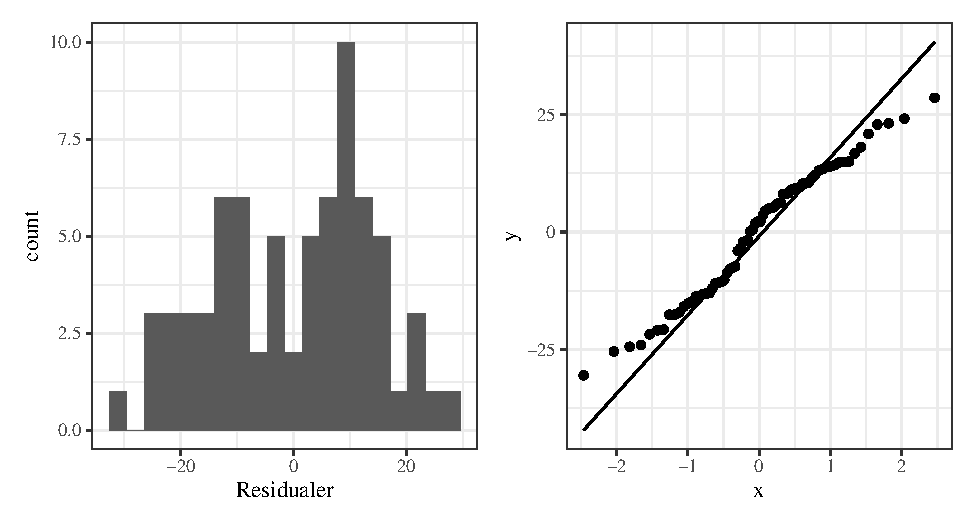
\includegraphics{R-anvisningar_files/figure-latex/unnamed-chunk-257-1} \end{center}

Punkterna avviker något från normalfördelningen i svansarna, men det är förstås alltid en bedömningsfråga.

Lika varians undersöks ofta med ett spridningsdiagram med de skattade värdena på x-axeln och residualerna på y-axeln.

\begin{Shaded}
\begin{Highlighting}[]
\FunctionTok{ggplot}\NormalTok{(oats, }\FunctionTok{aes}\NormalTok{(}\AttributeTok{x =}\NormalTok{ Skattade, }\AttributeTok{y =}\NormalTok{ Residualer)) }\SpecialCharTok{+}
  \FunctionTok{geom\_point}\NormalTok{() }\SpecialCharTok{+}
  \FunctionTok{geom\_hline}\NormalTok{(}\AttributeTok{yintercept =} \DecValTok{0}\NormalTok{, }\AttributeTok{alpha =} \FloatTok{0.3}\NormalTok{)}
\end{Highlighting}
\end{Shaded}

\begin{center}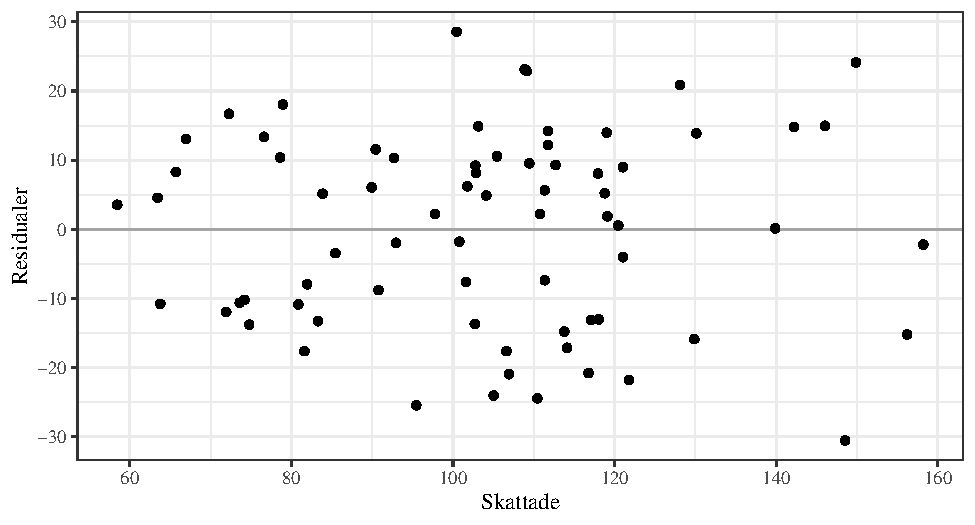
\includegraphics{R-anvisningar_files/figure-latex/unnamed-chunk-258-1} \end{center}

Om datan är i linje med antaganden ska diagrammet se ut som slumpmässigt placerade punkter med ungefär lika stor spridning kring noll-linjen för samtliga nivåer på x-axeln. För det här exemplet ser det okej ut.

\begin{exercise}[Bakterieimport]

Fliken \emph{Bakterier} i filen \emph{Uppgiftsdata.xlsx} innehåller data om tillväxt hos gräs efter inokulering av bakterier. Ladda ner filen och importera datan genom att fylla i koden nedan.

\begin{Shaded}
\begin{Highlighting}[]
\NormalTok{dat\_bact }\OtherTok{\textless{}{-}} \FunctionTok{read\_excel}\NormalTok{(}\StringTok{"\_\_\_"}\NormalTok{, }\AttributeTok{sheet =} \StringTok{"Bakterier"}\NormalTok{)}
\end{Highlighting}
\end{Shaded}

\end{exercise}

\begin{exercise}[Bakterieimport]

Illustrera datan med en lämplig graf, till exempel ett spridningsdiagram med \texttt{Inoculation} på x-axeln, \texttt{Dry\ weight} på y-axeln, småfönster efter \texttt{Cultivar} och färg efter \texttt{Block}.

\begin{Shaded}
\begin{Highlighting}[]
\FunctionTok{ggplot}\NormalTok{(dat\_bact, }\FunctionTok{aes}\NormalTok{(}\AttributeTok{x =}\NormalTok{ \_\_\_, }\AttributeTok{y =} \StringTok{\textasciigrave{}}\AttributeTok{\_\_\_}\StringTok{\textasciigrave{}}\NormalTok{, }\AttributeTok{color =}\NormalTok{ Block)) }\SpecialCharTok{+}
  \FunctionTok{geom\_point}\NormalTok{(}\AttributeTok{size =} \DecValTok{6}\NormalTok{) }\SpecialCharTok{+}
  \FunctionTok{facet\_wrap}\NormalTok{(}\SpecialCharTok{\textasciitilde{}}\NormalTok{ \_\_\_)}
\end{Highlighting}
\end{Shaded}

Hur blev färgerna för blocket? Om de inte blev distinkta färger kan variabeln \texttt{Block} ha blivit inläst som numerisk. Transformera variabeln med \texttt{as.character()} och gör om grafen. Ändras färgerna?

\begin{Shaded}
\begin{Highlighting}[]
\NormalTok{dat\_bact }\OtherTok{\textless{}{-}}\NormalTok{ dat\_bact }\SpecialCharTok{\%\textgreater{}\%} 
  \FunctionTok{mutate}\NormalTok{(}\AttributeTok{Block =} \FunctionTok{as.character}\NormalTok{(Block))}
\end{Highlighting}
\end{Shaded}

\end{exercise}

\begin{exercise}[Bakteriemodell]

Bakteriedatan har två faktorer och en blockfaktor. Skatta en anova-modell med interaktion och block genom att fylla i stycket nedan. Ta fram anovatabell och dra en slutsats från F-testen. Ligger slutsatsen i linje med grafen?

\begin{Shaded}
\begin{Highlighting}[]
\NormalTok{mod }\OtherTok{\textless{}{-}} \FunctionTok{lm}\NormalTok{(}\StringTok{\textasciigrave{}}\AttributeTok{\_\_\_}\StringTok{\textasciigrave{}} \SpecialCharTok{\textasciitilde{}}\NormalTok{ \_\_\_ }\SpecialCharTok{*}\NormalTok{ \_\_\_ }\SpecialCharTok{+}\NormalTok{ \_\_\_, }\AttributeTok{data =}\NormalTok{ dat\_bact)}
\FunctionTok{Anova}\NormalTok{(mod)}
\end{Highlighting}
\end{Shaded}

\end{exercise}

\begin{exercise}[Bakteriejämförelser]

Använd \texttt{emmeans()} för parvisa jämförelser mellan inokuleringsmetoder. Vilka par är signifikant åtskilda?

\begin{Shaded}
\begin{Highlighting}[]
\FunctionTok{emmeans}\NormalTok{(mod, pairwise }\SpecialCharTok{\textasciitilde{}}\NormalTok{ \_\_\_)}
\end{Highlighting}
\end{Shaded}

\end{exercise}

\begin{exercise}[Bakterieresidualer]
Vi använder den skattade modellen för att ta fram skattade värden och residualer.

\begin{Shaded}
\begin{Highlighting}[]
\NormalTok{dat\_bact }\OtherTok{\textless{}{-}}\NormalTok{ dat\_bact }\SpecialCharTok{\%\textgreater{}\%} 
  \FunctionTok{mutate}\NormalTok{(}\AttributeTok{Residualer =} \FunctionTok{residuals}\NormalTok{(mod),}
         \AttributeTok{Skattade =} \FunctionTok{fitted}\NormalTok{(mod))}
\end{Highlighting}
\end{Shaded}

Använd exemplet på residualtester ovan för att undersöka antagandet om normalfördelade residualer.
\end{exercise}

\section{Bonus. Statistik för ekologi}\label{bonus.-statistik-fuxf6r-ekologi}

Här tittar vi på några statistiska metoder som är vanliga inom ekologin, men går bortom materialet på en statistisk grundkurs. Vi börjar med datastruktur och visualisering för populationsdata, för att sedan titta på diversitetsmått, principalkomponentanalys (PCA) och hierarkisk klustering. Det vanligaste paketet för ekologi är \texttt{vegan}, så vi kan börja med att installera och ladda det. Vi kommer också använda \texttt{factoextra} för en graf.

\begin{Shaded}
\begin{Highlighting}[]
\CommentTok{\# install.packages("vegan")}
\FunctionTok{library}\NormalTok{(vegan)}

\CommentTok{\# install.packages("factoextra")}
\FunctionTok{library}\NormalTok{(factoextra)}
\end{Highlighting}
\end{Shaded}

Data för ekologiska populationer för flera platser eller tillfällen ordnas oftast i en tabell med plats som rad och arter som kolumner. Värdena i tabellen anger antingen antalet observerade individer eller ett binärt utfall (1 för förekomst, 0 för ingen förekomst). Exempeldatan \texttt{dune}, som kan laddas med funktionen \texttt{data()}, ger ett exempel. För att illustrera en typisk jämförelsestudie skapar vi en kolumn för platstyp och lägger till ett plats-id.

\begin{Shaded}
\begin{Highlighting}[]
\FunctionTok{data}\NormalTok{(dune)}
\NormalTok{dune }\OtherTok{\textless{}{-}}\NormalTok{ dune }\SpecialCharTok{\%\textgreater{}\%} 
  \FunctionTok{mutate}\NormalTok{(}\AttributeTok{Site =} \DecValTok{1}\SpecialCharTok{:}\FunctionTok{n}\NormalTok{(), }
         \AttributeTok{Type =} \FunctionTok{rep}\NormalTok{(}\FunctionTok{c}\NormalTok{(}\StringTok{"A"}\NormalTok{, }\StringTok{"B"}\NormalTok{), }\AttributeTok{each =} \DecValTok{10}\NormalTok{))}
\end{Highlighting}
\end{Shaded}

Vi kan illustrera data genom att pivotera till långt format och göra en graf med \texttt{ggplot()}. En heatmap eller ett spridningsdiagram med storlek för antal observationer kan vara lämpliga grafer. Tolkning kräver förstås kod artkännedom och beror på den vetenskapliga frågan.

\begin{Shaded}
\begin{Highlighting}[]
\NormalTok{dune\_long }\OtherTok{\textless{}{-}}\NormalTok{ dune }\SpecialCharTok{\%\textgreater{}\%}
  \FunctionTok{pivot\_longer}\NormalTok{(}\SpecialCharTok{{-}}\FunctionTok{c}\NormalTok{(Site, Type), }\AttributeTok{names\_to =} \StringTok{"Species"}\NormalTok{, }\AttributeTok{values\_to =} \StringTok{"Abundance"}\NormalTok{)}

\FunctionTok{ggplot}\NormalTok{(dune\_long, }\FunctionTok{aes}\NormalTok{(Site, Species, }\AttributeTok{fill =}\NormalTok{ Abundance)) }\SpecialCharTok{+}
  \FunctionTok{geom\_tile}\NormalTok{() }\SpecialCharTok{+}
  \FunctionTok{scale\_fill\_gradient2}\NormalTok{() }\SpecialCharTok{+}
  \FunctionTok{theme\_minimal}\NormalTok{()}
\end{Highlighting}
\end{Shaded}

\begin{center}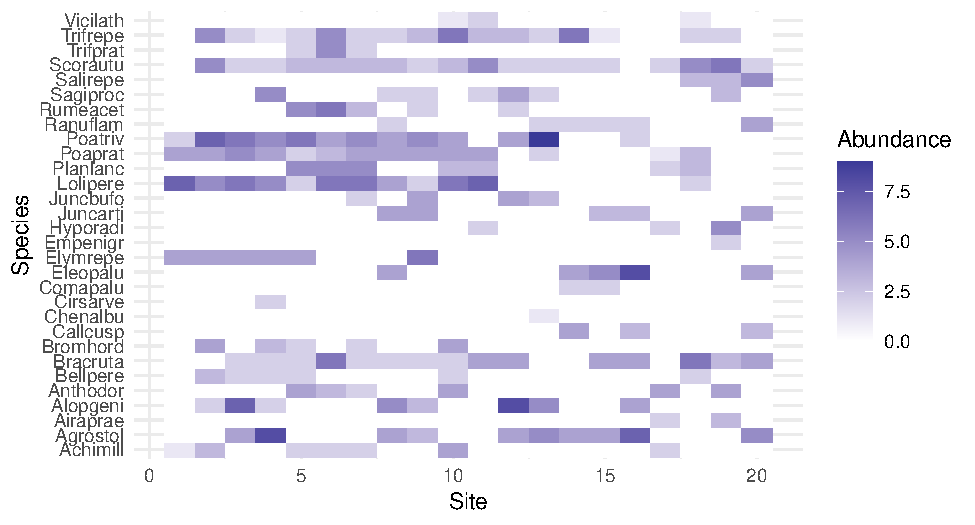
\includegraphics{R-anvisningar_files/figure-latex/unnamed-chunk-267-1} \end{center}

\begin{Shaded}
\begin{Highlighting}[]
\FunctionTok{ggplot}\NormalTok{(dune\_long }\SpecialCharTok{\%\textgreater{}\%} \FunctionTok{filter}\NormalTok{(Abundance }\SpecialCharTok{\textgreater{}} \DecValTok{0}\NormalTok{), }\FunctionTok{aes}\NormalTok{(Site, Species, }\AttributeTok{size =}\NormalTok{ Abundance, }\AttributeTok{color =}\NormalTok{ Type)) }\SpecialCharTok{+}
  \FunctionTok{geom\_point}\NormalTok{()}
\end{Highlighting}
\end{Shaded}

\begin{center}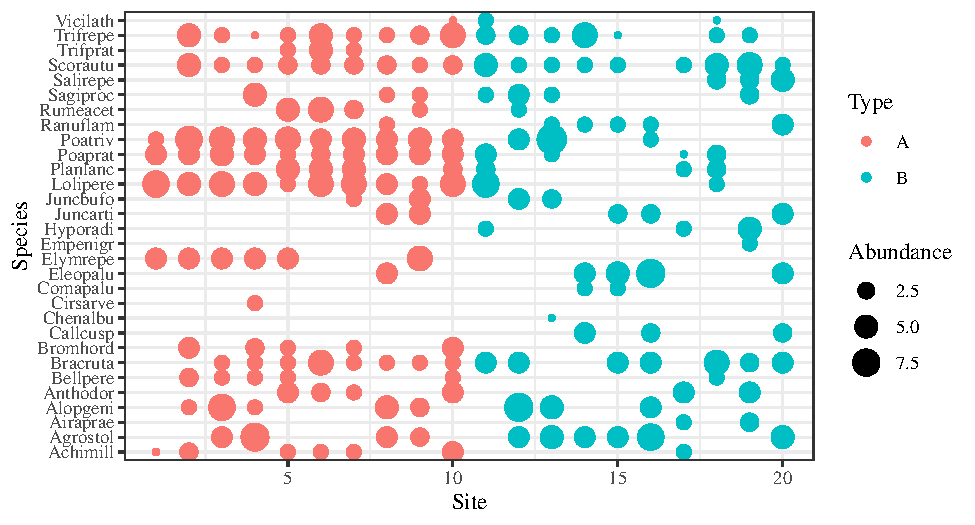
\includegraphics{R-anvisningar_files/figure-latex/unnamed-chunk-267-2} \end{center}

Ytterligare alternativ kan vara upprepade lådagram eller staplar med småfönster per art.

\begin{exercise}[Populationsgrafer]

Vad måste läggas till i stycket nedan för göra ett lådagram (med art på y-axeln och abundans på x-axeln) och ett stapeldiagram (med platstyp på x-axeln och abundans på y-axeln)?

\begin{Shaded}
\begin{Highlighting}[]
\NormalTok{dune\_long}
\FunctionTok{ggplot}\NormalTok{(dune\_long, }\FunctionTok{aes}\NormalTok{(}\AttributeTok{x =}\NormalTok{ \_\_\_, }\AttributeTok{y =}\NormalTok{ \_\_\_, }\AttributeTok{fill =}\NormalTok{ Type)) }\SpecialCharTok{+}
  \FunctionTok{geom\_boxplot}\NormalTok{()}

\FunctionTok{ggplot}\NormalTok{(dune\_long, }\FunctionTok{aes}\NormalTok{(}\AttributeTok{x =}\NormalTok{ \_\_\_, }\AttributeTok{y =}\NormalTok{ \_\_\_, }\AttributeTok{fill =}\NormalTok{ Type)) }\SpecialCharTok{+}
  \FunctionTok{geom\_col}\NormalTok{() }\SpecialCharTok{+}
  \FunctionTok{facet\_wrap}\NormalTok{(}\SpecialCharTok{\textasciitilde{}}\NormalTok{ \_\_\_, }\AttributeTok{nrow =} \DecValTok{2}\NormalTok{)}
\end{Highlighting}
\end{Shaded}

\end{exercise}

Ekologiska populationer kan analyseras genom \emph{heirarkisk klustring} - metoder där platser (rader) eller arter (kolumner) sorteras efter hur lika de är. Först beräknas ett avstånd mellan samtliga enheter (platser eller arter) och därefter sker klustringen genom att slå ihop enheter som ligger \emph{nära} varandra. Resultatet illustreras med ett träddiagram.

\begin{Shaded}
\begin{Highlighting}[]
\NormalTok{dune\_data }\OtherTok{\textless{}{-}}\NormalTok{ dune }\SpecialCharTok{\%\textgreater{}\%}\NormalTok{ dplyr}\SpecialCharTok{::}\FunctionTok{select}\NormalTok{(}\SpecialCharTok{{-}}\NormalTok{Site, }\SpecialCharTok{{-}}\NormalTok{Type)}
\NormalTok{d }\OtherTok{\textless{}{-}} \FunctionTok{dist}\NormalTok{(dune\_data, }\AttributeTok{method =} \StringTok{"euclidean"}\NormalTok{)}
\NormalTok{hc }\OtherTok{\textless{}{-}} \FunctionTok{hclust}\NormalTok{(d)}
\FunctionTok{plot}\NormalTok{(hc, }\AttributeTok{hang =} \SpecialCharTok{{-}}\DecValTok{1}\NormalTok{, }\AttributeTok{labels =}\NormalTok{ dune}\SpecialCharTok{$}\NormalTok{Type, }
     \AttributeTok{axes =}\NormalTok{ F, }\AttributeTok{xlab =} \StringTok{""}\NormalTok{, }\AttributeTok{ylab =} \StringTok{""}\NormalTok{, }\AttributeTok{ann =}\NormalTok{ F)}
\end{Highlighting}
\end{Shaded}

\begin{center}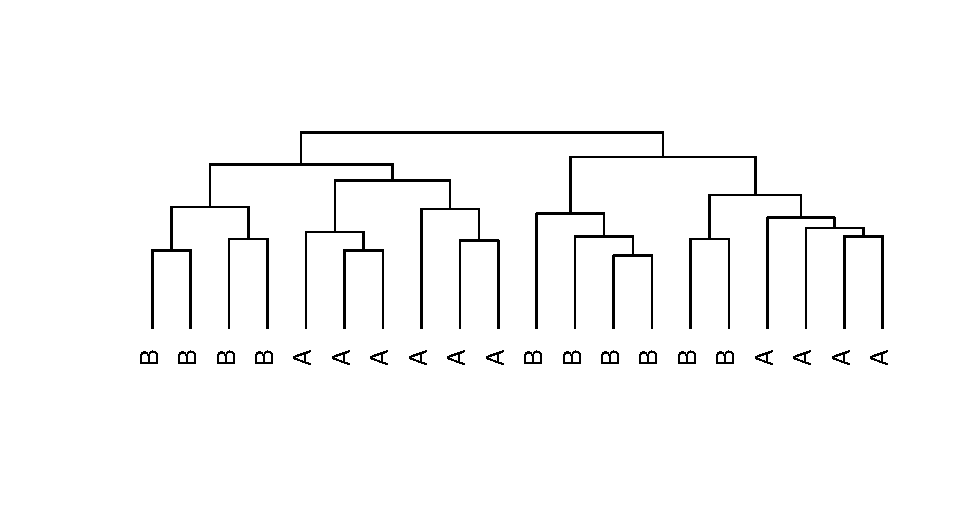
\includegraphics{R-anvisningar_files/figure-latex/unnamed-chunk-269-1} \end{center}

\begin{exercise}[Avståndsmått]
Ta upp hjälpsidan till distansfunktionen med \texttt{?dist}. Under \texttt{method} finns flera möjliga avståndsmått. Vad måste ändras i kodstycket ovan för att ange ett Manhattan-avstånd? Har avståndet någon betydande effekt på träddiagrammet?
\end{exercise}

För att göra en klustring av arter kan man \emph{transponera} data så att rader och kolumner byter plats med varandra. Här kommer artnamn automatisk med eftersom raderna i datan har namn. Det är inte alltid fallet, så det kan vara nödvändigt att sätta etiketter med argumentet \texttt{labels} i \texttt{plot()}.

\begin{Shaded}
\begin{Highlighting}[]
\NormalTok{dune\_data }\OtherTok{\textless{}{-}} \FunctionTok{t}\NormalTok{(dune\_data)}
\NormalTok{d }\OtherTok{\textless{}{-}} \FunctionTok{dist}\NormalTok{(dune\_data, }\AttributeTok{method =} \StringTok{"euclidean"}\NormalTok{)}
\NormalTok{hc }\OtherTok{\textless{}{-}} \FunctionTok{hclust}\NormalTok{(d)}
\FunctionTok{plot}\NormalTok{(hc, }\AttributeTok{hang =} \SpecialCharTok{{-}}\DecValTok{1}\NormalTok{,}
     \AttributeTok{axes =}\NormalTok{ F, }\AttributeTok{xlab =} \StringTok{""}\NormalTok{, }\AttributeTok{ylab =} \StringTok{""}\NormalTok{, }\AttributeTok{ann =}\NormalTok{ F)}
\end{Highlighting}
\end{Shaded}

\begin{center}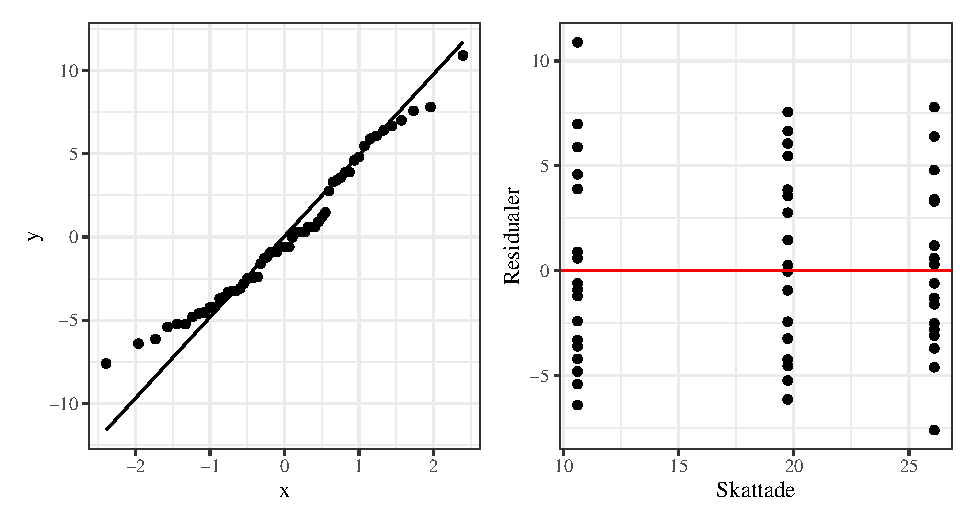
\includegraphics{R-anvisningar_files/figure-latex/unnamed-chunk-270-1} \end{center}

Träddiagrammet tolkas så att enheter vars koppling ligger lågt är mer lika varandra - arterna förekommer ofta på samma plats.

En annan vanlig metod för \emph{multivariat} data, vilket populationsdata är ett exempel på, är \emph{principalkomponentsanalys} (PCA, Principal Component Analysis). En PCA är ett försök att sammanfatta den ursprungliga datans 30 variabler (en per art) med ett mindre antal variabler. De nya variablerna - \emph{komponenterna} - skapas genom att väga och addera de ursprungliga variablerna på ett sätt som förklarar så mycket som möjligt av variationen med minsta möjliga antal variabler. Resultatet illustreras vanligen med en \emph{biplot} - ett spridningsdiagram som placerar ut både platser och arter.

I R kan en PCA göras med \texttt{prcomp()} och en biplot kan göras med \texttt{fviz\_pca\_biplot()} från \texttt{factoextra}.

\begin{Shaded}
\begin{Highlighting}[]
\NormalTok{dune\_data }\OtherTok{\textless{}{-}}\NormalTok{ dune }\SpecialCharTok{\%\textgreater{}\%}\NormalTok{ dplyr}\SpecialCharTok{::}\FunctionTok{select}\NormalTok{(}\SpecialCharTok{{-}}\NormalTok{Site, }\SpecialCharTok{{-}}\NormalTok{Type)}
\NormalTok{pca }\OtherTok{\textless{}{-}} \FunctionTok{prcomp}\NormalTok{(dune\_data, }\AttributeTok{scale. =}\NormalTok{ F)}
\FunctionTok{fviz\_pca\_biplot}\NormalTok{(pca, }\AttributeTok{geom.ind =} \StringTok{"point"}\NormalTok{, }\AttributeTok{habillage =}\NormalTok{ dune}\SpecialCharTok{$}\NormalTok{Type, }\AttributeTok{labelsize =} \DecValTok{3}\NormalTok{)}
\end{Highlighting}
\end{Shaded}

\begin{center}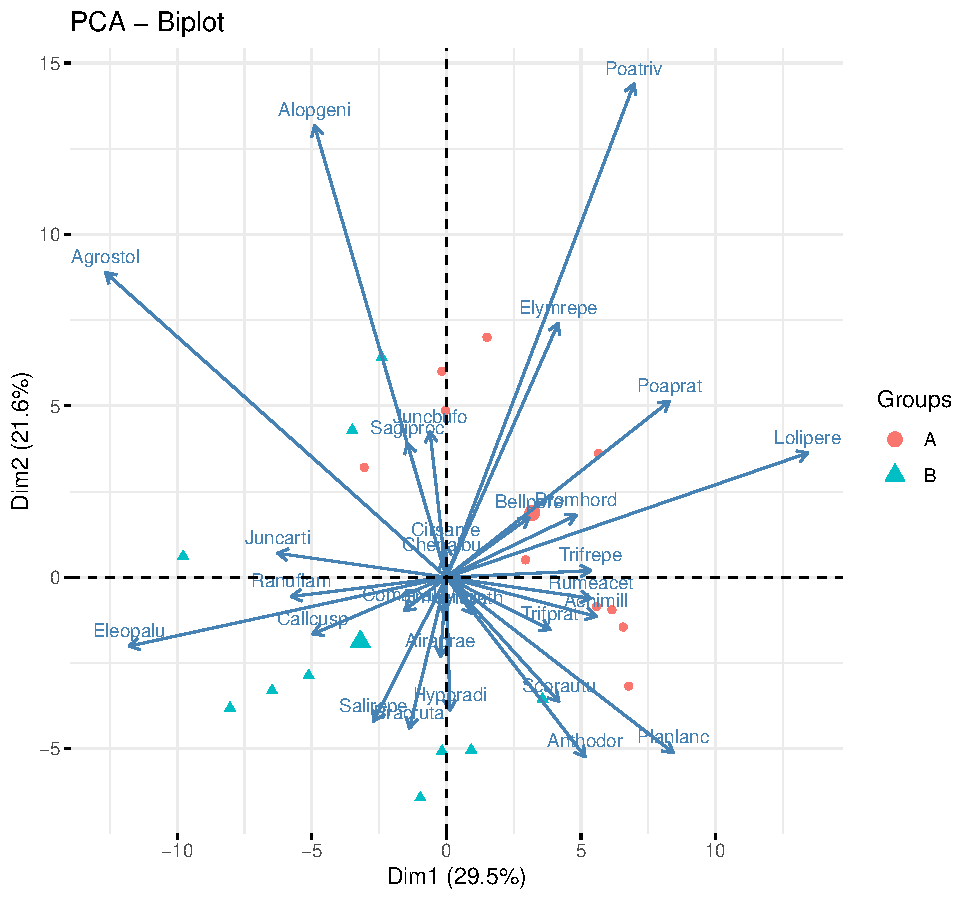
\includegraphics{R-anvisningar_files/figure-latex/unnamed-chunk-271-1} \end{center}

Platserna illustreras med punkter och arterna med pilar. Pilar i samma riktning motsvarar arter som är lika (de finns på samma platser), närliggande punkter motsvarar lika platser (de har samma arter), och punkter i samma riktning som en pil har höga värden för den arten.

\begin{exercise}[Skalning i en PCA]
En PCA kan göras med och utan att skala variablerna. Om variablerna skalas får en variabel som varierar mycket samma vikt som en variabel som varierar lite. Det kan vara bra om man har variabler som är mätta på olika sätt, till exempel om en variabel är i meter och en är i centimeter. Gör lämplig ändring i kodstycket ovan för att skala variablerna i \texttt{prcomp()}. Har det någon effekt på grafen?
\end{exercise}

Den sista ansatsen vi ska titta på är att sammanfatta en population i ett enskilt tal - ett diversitetsindex. Genom att beräkna ett index kan man reducera datan till en observation på plats. Man kan därifrån tillämpa de metoder vi sett i övriga delar av kursen (t-test och variansanalys). Det finns en stor mängd olika index. Det vanligaste än Shannon-Weaver indexet (eller entropi), vilket beräknas genom att ta andelen per art, multiplicera med logaritmen av andelen, summera över arter, och multiplicera med minus ett. Om man har tre arter med andelarna 0.3, 0.5 och 0.2 ges Shannon-Weaver alltså av

\begin{Shaded}
\begin{Highlighting}[]
\SpecialCharTok{{-}}\NormalTok{(}\FloatTok{0.3} \SpecialCharTok{*} \FunctionTok{log}\NormalTok{(}\FloatTok{0.3}\NormalTok{) }\SpecialCharTok{+} \FloatTok{0.5} \SpecialCharTok{*} \FunctionTok{log}\NormalTok{(}\FloatTok{0.5}\NormalTok{) }\SpecialCharTok{+} \FloatTok{0.2} \SpecialCharTok{*} \FunctionTok{log}\NormalTok{(}\FloatTok{0.2}\NormalTok{))}
\end{Highlighting}
\end{Shaded}

\begin{verbatim}
## [1] 1.029653
\end{verbatim}

Indexet ökar om det finns många arter och om andelen per art är samma. En population med \emph{en} dominant art kommer alltså ha ett lågt index.

För en tabell med data kan index beräknas med \texttt{diversity()}.

\begin{Shaded}
\begin{Highlighting}[]
\NormalTok{diver }\OtherTok{\textless{}{-}} \FunctionTok{diversity}\NormalTok{(dune\_data, }\AttributeTok{index =} \StringTok{"shannon"}\NormalTok{)}
\NormalTok{dune }\OtherTok{\textless{}{-}}\NormalTok{ dune }\SpecialCharTok{\%\textgreater{}\%} \FunctionTok{mutate}\NormalTok{(}\AttributeTok{Diversity =}\NormalTok{ diver)}
\end{Highlighting}
\end{Shaded}

Diversitetsindexen kan sedan illustreras och analyseras som vilken numerisk variabel som helst.

\begin{Shaded}
\begin{Highlighting}[]
\FunctionTok{ggplot}\NormalTok{(dune, }\FunctionTok{aes}\NormalTok{(Diversity, Type)) }\SpecialCharTok{+} \FunctionTok{geom\_point}\NormalTok{()}
\end{Highlighting}
\end{Shaded}

\begin{center}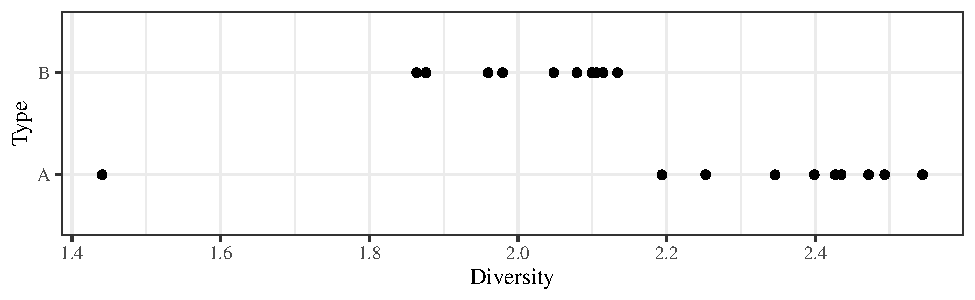
\includegraphics{R-anvisningar_files/figure-latex/unnamed-chunk-274-1} \end{center}

\begin{Shaded}
\begin{Highlighting}[]
\NormalTok{mod }\OtherTok{\textless{}{-}} \FunctionTok{lm}\NormalTok{(Diversity }\SpecialCharTok{\textasciitilde{}}\NormalTok{ Type, }\AttributeTok{data =}\NormalTok{ dune)}
\FunctionTok{Anova}\NormalTok{(mod)}
\end{Highlighting}
\end{Shaded}

\begin{verbatim}
## Anova Table (Type II tests)
## 
## Response: Diversity
##            Sum Sq Df F value  Pr(>F)  
## Type      0.37586  1  6.6647 0.01881 *
## Residuals 1.01513 18                  
## ---
## Signif. codes:  0 '***' 0.001 '**' 0.01 '*' 0.05 '.' 0.1 ' ' 1
\end{verbatim}

\begin{Shaded}
\begin{Highlighting}[]
\FunctionTok{emmeans}\NormalTok{(mod, }\SpecialCharTok{\textasciitilde{}}\NormalTok{ Type)}
\end{Highlighting}
\end{Shaded}

\begin{verbatim}
##  Type emmean     SE df lower.CL upper.CL
##  A      2.30 0.0751 18     2.14     2.46
##  B      2.03 0.0751 18     1.87     2.18
## 
## Confidence level used: 0.95
\end{verbatim}

Här finns en signifikant skillnad med platstyper.

\begin{exercise}[Diversitetsindex]
Ta upp hjälpsidan till funktionen \texttt{diversity()}. Hur anger man att funktionen ska ge Simpsons index?
\end{exercise}

\begin{exercise}[Test på nytt index]
Gör om analysen på diversitet (anovamodellen och F-testet) med Simpsons index istället för Shannon-Weaver. Påverkar valet av diversitetsindex utfallet av testet?
\end{exercise}

\chapter{Regression och korrelation}\label{regression-och-korrelation}

Datorövning 7 handlar om regression och korrelation. Efter övningen ska vi kunna

\begin{itemize}
\item
  skatta en regressionsmodell i R,
\item
  testa parametrar i modellen med F-test och t-test,
\item
  göra lämpliga tester av modellantaganden,
\item
  beräkna och tolka korrelationen mellan två variabler.
\end{itemize}

\section{Repetition av datorövning 6}\label{repetition-av-datoruxf6vning-6}

När man startar en ny R-session bör man ladda de paket man vet kommer behövas med \texttt{library()}. Om paket inte finns installerade måste man först köra \texttt{install.packages()}.

\begin{Shaded}
\begin{Highlighting}[]
\CommentTok{\# install.packages("tidyverse")}
\FunctionTok{library}\NormalTok{(tidyverse)}
\end{Highlighting}
\end{Shaded}

I datorövning 7 tittade vi på variansanalys - en metod som gör det möjligt att utvidga t-testet för två grupper till ett godtyckligt antal grupper eller kombinationer av faktorer. I variansanalys skattar man en modell som förklarar ett datautfall. Utifrån modellen sätter man upp en anova-tabell som delar upp den totala variansen i en förklarad del och en kvarvarande residualdel. Anova-tabell ger också ett F-test som testar om det finns några skillnader mellan grupper. Från en skattad modell kan man sedan göra parvisa jämförelser mellan specifika grupper och testa modellantaganden (främst antagande om normalfördelning och lika varians inom grupper).

Ta som exempel följande data på tandtillväxt (\texttt{len}) hos marsvin under C-vitaminbehandling i olika doser (\texttt{dose}) och två olika metoder (\texttt{supp}), tillgängligt i R som objektet \texttt{ToothGrowth}.

\begin{Shaded}
\begin{Highlighting}[]
\NormalTok{ToothGrowth }\OtherTok{\textless{}{-}}\NormalTok{ ToothGrowth }\SpecialCharTok{\%\textgreater{}\%} \FunctionTok{mutate}\NormalTok{(}\AttributeTok{dose =} \FunctionTok{as.character}\NormalTok{(dose))}

\FunctionTok{ggplot}\NormalTok{(ToothGrowth, }\FunctionTok{aes}\NormalTok{(len, supp, }\AttributeTok{fill =}\NormalTok{ dose)) }\SpecialCharTok{+} 
  \FunctionTok{geom\_boxplot}\NormalTok{()}
\end{Highlighting}
\end{Shaded}

\begin{center}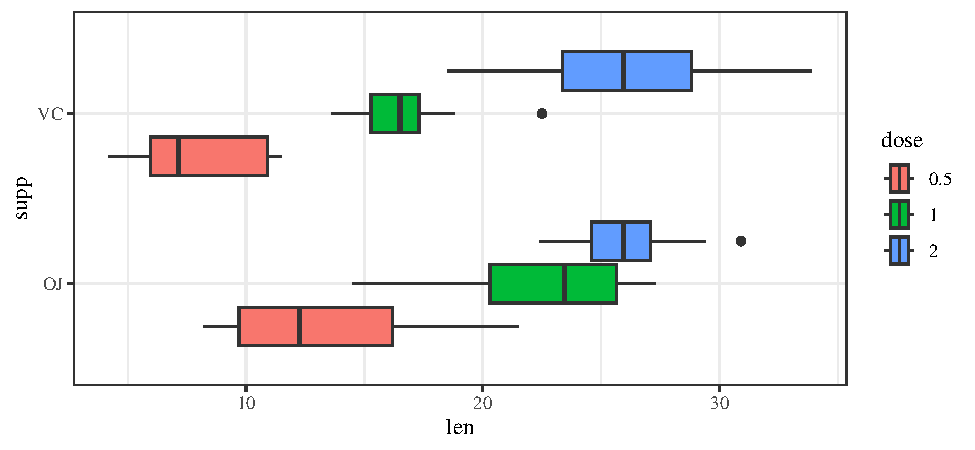
\includegraphics{R-anvisningar_files/figure-latex/unnamed-chunk-276-1} \end{center}

Ett lådagram visar en klar skillnad mellan doser och en svagare skillnad mellan metoder. Det finns också tecken på att metoderna svarar olika på dos i att metoden \emph{VC} ligger lägre än \emph{OJ} vid de låga doserna men över (eller iallafall lika) vid den höga dosen.

En envägsanova-modell (en modell med en faktor) kan skattas med \texttt{lm()} och en anovatabell kan tas fram med \texttt{Anova()} från paketet \texttt{car}.

\begin{Shaded}
\begin{Highlighting}[]
\NormalTok{mod }\OtherTok{\textless{}{-}} \FunctionTok{lm}\NormalTok{(len }\SpecialCharTok{\textasciitilde{}}\NormalTok{ dose, }\AttributeTok{data =}\NormalTok{ ToothGrowth)}

\FunctionTok{library}\NormalTok{(car)}
\FunctionTok{Anova}\NormalTok{(mod)}
\end{Highlighting}
\end{Shaded}

\begin{verbatim}
## Anova Table (Type II tests)
## 
## Response: len
##           Sum Sq Df F value    Pr(>F)    
## dose      2426.4  2  67.416 9.533e-16 ***
## Residuals 1025.8 57                      
## ---
## Signif. codes:  0 '***' 0.001 '**' 0.01 '*' 0.05 '.' 0.1 ' ' 1
\end{verbatim}

F-testets nollhypotes är att alla grupper (här alla doser) har samma populationsmedelvärde. Det låga p-värdet pekar på en klar skillnad mellan doser.

En anovamodell bygger på antaganden om normalfördelning och lika varianser. Normalfördelningsantagandet kan undersökas med en QQ-graf över residualerna och variansantagandet kan undersökas med en spridningsgraf över skattade värden och residualer.

\begin{Shaded}
\begin{Highlighting}[]
\FunctionTok{library}\NormalTok{(patchwork)}
\NormalTok{ToothGrowth }\OtherTok{\textless{}{-}}\NormalTok{ ToothGrowth }\SpecialCharTok{\%\textgreater{}\%} 
  \FunctionTok{mutate}\NormalTok{(}\AttributeTok{Skattade =} \FunctionTok{fitted}\NormalTok{(mod),}
         \AttributeTok{Residualer =} \FunctionTok{residuals}\NormalTok{(mod))}
\NormalTok{g1 }\OtherTok{\textless{}{-}} \FunctionTok{ggplot}\NormalTok{(ToothGrowth, }\FunctionTok{aes}\NormalTok{(}\AttributeTok{sample =}\NormalTok{ Residualer)) }\SpecialCharTok{+} \FunctionTok{geom\_qq}\NormalTok{() }\SpecialCharTok{+} \FunctionTok{geom\_qq\_line}\NormalTok{()}
\NormalTok{g2 }\OtherTok{\textless{}{-}} \FunctionTok{ggplot}\NormalTok{(ToothGrowth, }\FunctionTok{aes}\NormalTok{(Skattade, Residualer)) }\SpecialCharTok{+}
  \FunctionTok{geom\_point}\NormalTok{() }\SpecialCharTok{+}
  \FunctionTok{geom\_hline}\NormalTok{(}\AttributeTok{yintercept =} \DecValTok{0}\NormalTok{, }\AttributeTok{color =} \StringTok{"red"}\NormalTok{)}
\NormalTok{g1 }\SpecialCharTok{+}\NormalTok{ g2}
\end{Highlighting}
\end{Shaded}

\begin{center}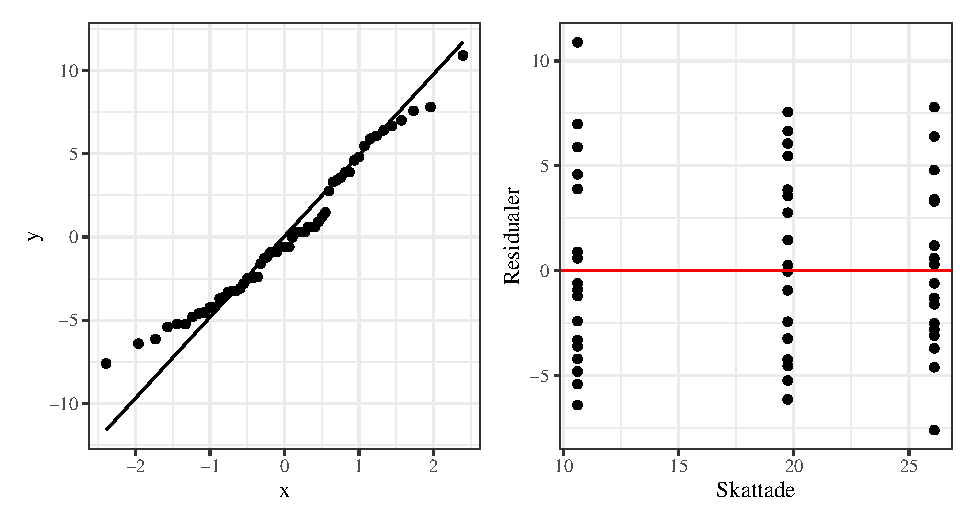
\includegraphics{R-anvisningar_files/figure-latex/unnamed-chunk-278-1} \end{center}

Punkterna ligger ungefär på linjen i QQ-grafen och punkterna har ungefär samma spridning för alla nivåer av det skattade värdet.

Anova-modeller kan lätt byggas ut genom att lägga till fler faktorer. Här är det till exempel naturligt att skatta en modell med både metod och dos, vilket kan göras genom att lägga till \texttt{supp} till formeln i \texttt{lm()}.

\begin{Shaded}
\begin{Highlighting}[]
\NormalTok{mod }\OtherTok{\textless{}{-}} \FunctionTok{lm}\NormalTok{(len }\SpecialCharTok{\textasciitilde{}}\NormalTok{ dose }\SpecialCharTok{*}\NormalTok{ supp, ToothGrowth)}
\FunctionTok{Anova}\NormalTok{(mod)}
\end{Highlighting}
\end{Shaded}

\begin{verbatim}
## Anova Table (Type II tests)
## 
## Response: len
##            Sum Sq Df F value    Pr(>F)    
## dose      2426.43  2  92.000 < 2.2e-16 ***
## supp       205.35  1  15.572 0.0002312 ***
## dose:supp  108.32  2   4.107 0.0218603 *  
## Residuals  712.11 54                      
## ---
## Signif. codes:  0 '***' 0.001 '**' 0.01 '*' 0.05 '.' 0.1 ' ' 1
\end{verbatim}

Resultaten är i linje med grafen - dos har en stor effekt medan metod och interaktionen mellan dos och metod är något svagare, om än signifikanta.

En anovamodell kan användas för parvisa jämförelse, vilket ibland kallas post-hoc-test. Den vanligaste är Tukey-testet, men andra tester kan också förekomma. Testet kan utföras med \texttt{emmeans()} från paketet med samma namn. Följande ger en jämförelse mellan doser uppdelat efter metod.

\begin{Shaded}
\begin{Highlighting}[]
\FunctionTok{library}\NormalTok{(emmeans)}
\FunctionTok{emmeans}\NormalTok{(mod, pairwise }\SpecialCharTok{\textasciitilde{}}\NormalTok{ dose }\SpecialCharTok{|}\NormalTok{ supp)}
\end{Highlighting}
\end{Shaded}

\begin{verbatim}
## $emmeans
## supp = OJ:
##  dose emmean   SE df lower.CL upper.CL
##  0.5   13.23 1.15 54    10.93     15.5
##  1     22.70 1.15 54    20.40     25.0
##  2     26.06 1.15 54    23.76     28.4
## 
## supp = VC:
##  dose emmean   SE df lower.CL upper.CL
##  0.5    7.98 1.15 54     5.68     10.3
##  1     16.77 1.15 54    14.47     19.1
##  2     26.14 1.15 54    23.84     28.4
## 
## Confidence level used: 0.95 
## 
## $contrasts
## supp = OJ:
##  contrast        estimate   SE df t.ratio p.value
##  dose0.5 - dose1    -9.47 1.62 54  -5.831  <.0001
##  dose0.5 - dose2   -12.83 1.62 54  -7.900  <.0001
##  dose1 - dose2      -3.36 1.62 54  -2.069  0.1060
## 
## supp = VC:
##  contrast        estimate   SE df t.ratio p.value
##  dose0.5 - dose1    -8.79 1.62 54  -5.413  <.0001
##  dose0.5 - dose2   -18.16 1.62 54 -11.182  <.0001
##  dose1 - dose2      -9.37 1.62 54  -5.770  <.0001
## 
## P value adjustment: tukey method for comparing a family of 3 estimates
\end{verbatim}

\section{Regression}\label{regression}

I en regression modelleras en numerisk variabel som en funktion av en annan numerisk variabel. Vid enkel linjär regression finns \emph{en} sådan \emph{förklarande variabel} och förhållandet mellan variablerna antas vara linjärt.

Ta som exempel data på förväntad medellivslängd och bnp per capita. Datan hämtas från \texttt{gapminder}-paketet. Paketet \texttt{ggrepel} och funktionen \texttt{geom\_text\_repel()} kan användas för att sätta punktetiketter som inte överlappar. För enklare tolkning av modellen transformeras bnp per capita till att vara i tusen dollar, snarare än dollar.

\begin{Shaded}
\begin{Highlighting}[]
\FunctionTok{library}\NormalTok{(gapminder)}
\NormalTok{dat\_eu07 }\OtherTok{\textless{}{-}}\NormalTok{ gapminder }\SpecialCharTok{\%\textgreater{}\%} 
  \FunctionTok{filter}\NormalTok{(year }\SpecialCharTok{==} \DecValTok{2007}\NormalTok{, continent }\SpecialCharTok{==} \StringTok{"Europe"}\NormalTok{) }\SpecialCharTok{\%\textgreater{}\%} 
  \FunctionTok{mutate}\NormalTok{(}\AttributeTok{gdpPercap =}\NormalTok{ gdpPercap }\SpecialCharTok{/} \DecValTok{1000}\NormalTok{)}

\FunctionTok{library}\NormalTok{(ggrepel)}
\FunctionTok{ggplot}\NormalTok{(dat\_eu07, }\FunctionTok{aes}\NormalTok{(gdpPercap, lifeExp)) }\SpecialCharTok{+}
  \FunctionTok{geom\_point}\NormalTok{() }\SpecialCharTok{+}
  \FunctionTok{geom\_text\_repel}\NormalTok{(}\FunctionTok{aes}\NormalTok{(}\AttributeTok{label =}\NormalTok{ country), }\AttributeTok{size =} \DecValTok{3}\NormalTok{)}
\end{Highlighting}
\end{Shaded}

\begin{center}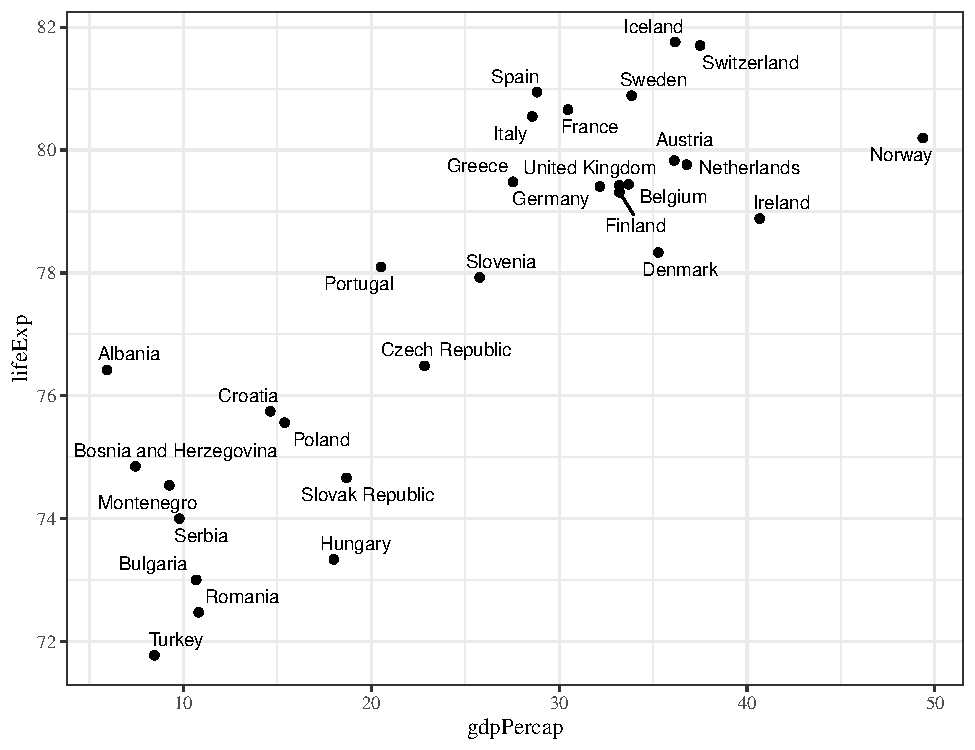
\includegraphics{R-anvisningar_files/figure-latex/unnamed-chunk-281-1} \end{center}

Datan visar ett positivt samband mellan variablerna - högre bnp per capita är kopplat till högre medellivslängd.

\begin{exercise}[Data för 1957]

Vad måste ändras i stycket nedan för att plocka ut data och göra en graf för Europa 1957?

\begin{Shaded}
\begin{Highlighting}[]
\NormalTok{dat\_eu57 }\OtherTok{\textless{}{-}}\NormalTok{ gapminder }\SpecialCharTok{\%\textgreater{}\%} 
  \FunctionTok{filter}\NormalTok{(year }\SpecialCharTok{==} \DecValTok{2007}\NormalTok{, continent }\SpecialCharTok{==} \StringTok{"Europe"}\NormalTok{) }\SpecialCharTok{\%\textgreater{}\%} 
  \FunctionTok{mutate}\NormalTok{(}\AttributeTok{gdpPercap =}\NormalTok{ gdpPercap }\SpecialCharTok{/} \DecValTok{1000}\NormalTok{)}

\FunctionTok{ggplot}\NormalTok{(dat\_eu57, }\FunctionTok{aes}\NormalTok{(gdpPercap, lifeExp)) }\SpecialCharTok{+}
  \FunctionTok{geom\_point}\NormalTok{() }\SpecialCharTok{+}
  \FunctionTok{geom\_text\_repel}\NormalTok{(}\FunctionTok{aes}\NormalTok{(}\AttributeTok{label =}\NormalTok{ country), }\AttributeTok{size =} \DecValTok{3}\NormalTok{)}
\end{Highlighting}
\end{Shaded}

\end{exercise}

En regressionmodell kan i R skattas med \texttt{lm}-funktionen. Syntaxen är väldigt lik den för anovamodellen, men istället för en faktor som förklarande variabel används nu en kontinuerlig variabel.

\begin{Shaded}
\begin{Highlighting}[]
\NormalTok{mod }\OtherTok{\textless{}{-}} \FunctionTok{lm}\NormalTok{(lifeExp }\SpecialCharTok{\textasciitilde{}}\NormalTok{ gdpPercap, }\AttributeTok{data =}\NormalTok{ dat\_eu07)}
\FunctionTok{summary}\NormalTok{(mod)}
\end{Highlighting}
\end{Shaded}

\begin{verbatim}
## 
## Call:
## lm(formula = lifeExp ~ gdpPercap, data = dat_eu07)
## 
## Residuals:
##      Min       1Q   Median       3Q      Max 
## -2.79839 -1.30472  0.00807  1.33443  2.87766 
## 
## Coefficients:
##             Estimate Std. Error t value Pr(>|t|)    
## (Intercept) 72.27106    0.69416 104.113  < 2e-16 ***
## gdpPercap    0.21463    0.02514   8.537  2.8e-09 ***
## ---
## Signif. codes:  0 '***' 0.001 '**' 0.01 '*' 0.05 '.' 0.1 ' ' 1
## 
## Residual standard error: 1.598 on 28 degrees of freedom
## Multiple R-squared:  0.7225, Adjusted R-squared:  0.7125 
## F-statistic: 72.88 on 1 and 28 DF,  p-value: 2.795e-09
\end{verbatim}

Funktionen \texttt{summary} ger en sammanfattning av modellen. Skattningen av modellens konstanta parameter ges som raden \texttt{(Intercept)} och dess tolkning är som förväntat värde i medellivslängd om bnp per capita är noll. Det är ofta lutningsparametern som är mer intressant. Skattningen av lutningsparametern ges på den rad som har samma namn som den förklarande variabeln, här \texttt{gdpPercap}. Den skattade parametern är 0.2146. Lutningsparametern har den generella tolkning som ökningen i y-variabeln när x-variabeln ökar med 1. I det här fallet ger 0.2146 att ett lands medellivslängd ökar med ungefär 0.2146 år (eller 78 dagar) när bnp per capita ökar med 1000 dollar.

\begin{exercise}[Modell för 1957]
Skatta samma modell som ovan, denna gång med data från 1957. Tolka lutningsparametern i ord. Är effekten av ökad bnp större 2007 än den var 1957?
\end{exercise}

Man kan enkelt rita ut regressionlinjen i en graf med \texttt{geom\_smooth()} och argumentet \texttt{method} satt till \texttt{lm}.

\begin{Shaded}
\begin{Highlighting}[]
\FunctionTok{ggplot}\NormalTok{(dat\_eu07, }\FunctionTok{aes}\NormalTok{(gdpPercap, lifeExp)) }\SpecialCharTok{+}
  \FunctionTok{geom\_point}\NormalTok{() }\SpecialCharTok{+}
  \FunctionTok{geom\_text\_repel}\NormalTok{(}\FunctionTok{aes}\NormalTok{(}\AttributeTok{label =}\NormalTok{ country), }\AttributeTok{size =} \DecValTok{3}\NormalTok{) }\SpecialCharTok{+}
  \FunctionTok{geom\_smooth}\NormalTok{(}\AttributeTok{method =}\NormalTok{ lm)}
\end{Highlighting}
\end{Shaded}

\begin{center}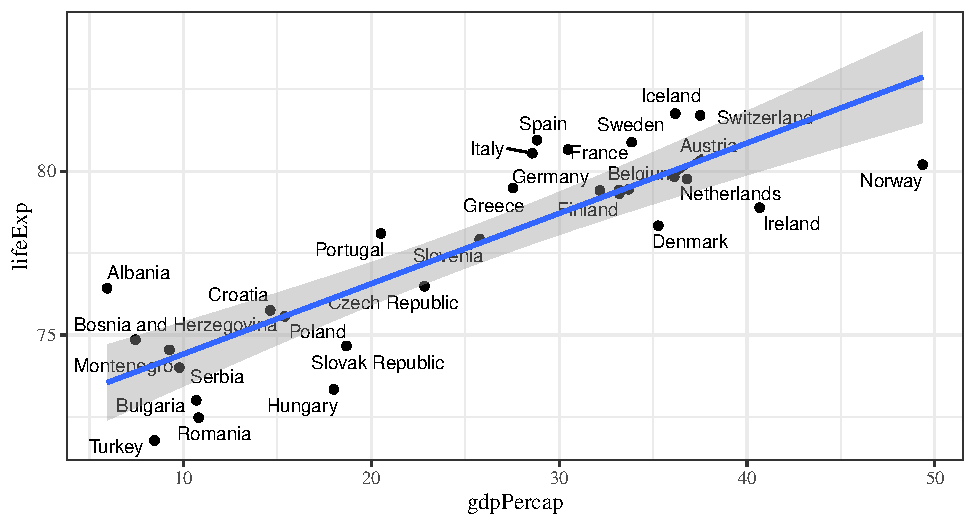
\includegraphics{R-anvisningar_files/figure-latex/unnamed-chunk-284-1} \end{center}

Den blå linjen illustrerar regressionlinjen 72.27 + 0.2146x. Det grå bandet kring linjen är ett konfidensintervall för skattningen av y-variabeln.

\begin{exercise}[Graf för 1957]
Använd \texttt{geom\_smooth(method\ =\ lm)} för att lägga till en regressionslinje för data för 1957. Hur mycket påverkar de två avvikande länderna?
\end{exercise}

Utskriften från \texttt{summary} ger också tester av parametrarna (den högra kolumnen \texttt{Pr(\textgreater{}\textbar{}t\textbar{})} ger p-värdet för ett test där nollhypotesen är att populationsparametern är noll). I det här fallet är både intercept och lutning skilda från noll. Motsvarande F-test för lutningen kan tas fram med en anova-tabell.

\begin{Shaded}
\begin{Highlighting}[]
\FunctionTok{library}\NormalTok{(car)}
\FunctionTok{Anova}\NormalTok{(mod)}
\end{Highlighting}
\end{Shaded}

\begin{verbatim}
## Anova Table (Type II tests)
## 
## Response: lifeExp
##            Sum Sq Df F value    Pr(>F)    
## gdpPercap 186.031  1  72.883 2.795e-09 ***
## Residuals  71.469 28                      
## ---
## Signif. codes:  0 '***' 0.001 '**' 0.01 '*' 0.05 '.' 0.1 ' ' 1
\end{verbatim}

Testerna av en regressionsmodell bygger på ett normalfördelningsantagande och ett antagande om \emph{homoskedasticitet} (lika varians i y oavsett position på x-axeln). Antagandena kan undersökas genom att titta på skattningens \emph{residualer} - skillnaden mellan det faktiska y-värdet och modellens värde. Residualerna kan undersökas med ett histogram eller en QQ-plot. En annan vanlig diagnosplot är ett spridningsdiagram med skattade värden på x-axeln och residualerna på y-axeln.

\begin{Shaded}
\begin{Highlighting}[]
\NormalTok{dat\_eu07 }\OtherTok{\textless{}{-}}\NormalTok{ dat\_eu07 }\SpecialCharTok{\%\textgreater{}\%} 
  \FunctionTok{mutate}\NormalTok{(}\AttributeTok{Residualer =} \FunctionTok{residuals}\NormalTok{(mod),}
         \AttributeTok{Skattade =} \FunctionTok{fitted}\NormalTok{(mod))}

\FunctionTok{ggplot}\NormalTok{(dat\_eu07, }\FunctionTok{aes}\NormalTok{(}\AttributeTok{sample =}\NormalTok{ Residualer)) }\SpecialCharTok{+} \FunctionTok{geom\_qq}\NormalTok{() }\SpecialCharTok{+} \FunctionTok{geom\_qq\_line}\NormalTok{()}
\end{Highlighting}
\end{Shaded}

\begin{center}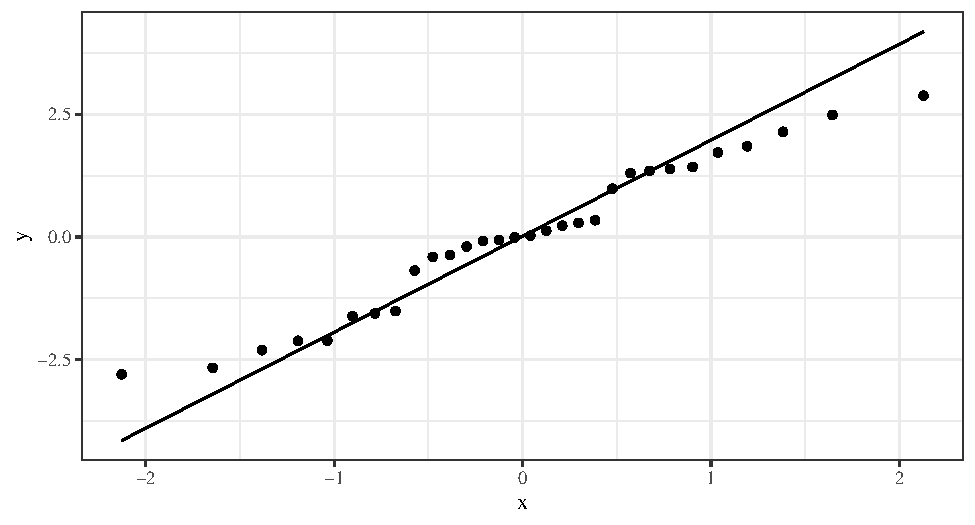
\includegraphics{R-anvisningar_files/figure-latex/unnamed-chunk-286-1} \end{center}

\begin{Shaded}
\begin{Highlighting}[]
\FunctionTok{ggplot}\NormalTok{(dat\_eu07, }\FunctionTok{aes}\NormalTok{(Skattade, Residualer)) }\SpecialCharTok{+} \FunctionTok{geom\_point}\NormalTok{()}
\end{Highlighting}
\end{Shaded}

\begin{center}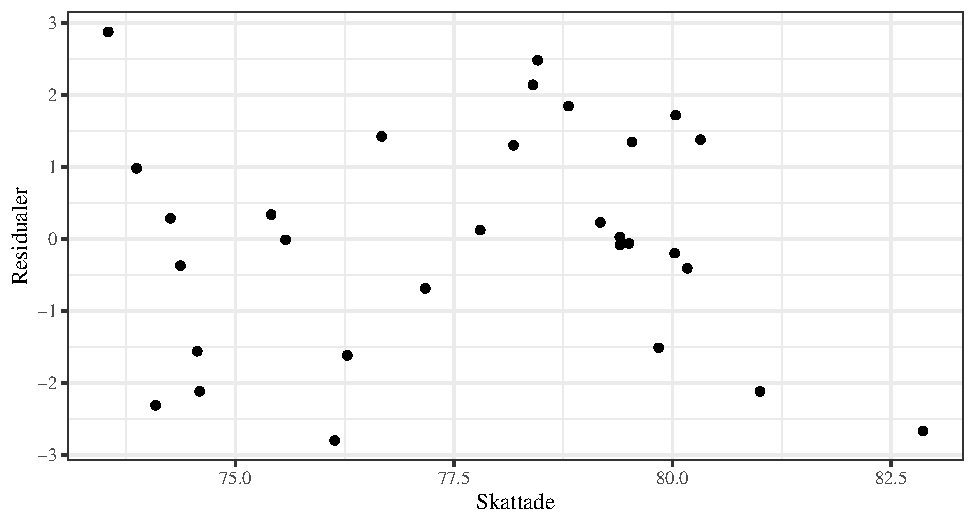
\includegraphics{R-anvisningar_files/figure-latex/unnamed-chunk-286-2} \end{center}

Om data följer en normalfördelning bör histogrammet visa en ungefärlig normalkurva, QQ-plotten bör visa punkter på den diagonala linjen och spridningsdiagrammet bör visa en slumpmässig spridning av punkter. Graferna pekar i det här fallet inte på några tydliga avvikelser från normalfördelningsantagandet, möjligen pekar QQ-plotten på mindre spridning i svansarna än en teoretisk normalfördelning.

\begin{exercise}[Diagnos för 1957]
Gör lämpliga ändringar i data ovan för diagnosgrafer för data från 1957. Finns det några tydliga avvikande värden?
\end{exercise}

\begin{exercise}[Icke-linjära samband]
Låt oss titta på hela gapminder-datan för 2007.

\begin{Shaded}
\begin{Highlighting}[]
\NormalTok{dat\_2007 }\OtherTok{\textless{}{-}}\NormalTok{ gapminder }\SpecialCharTok{\%\textgreater{}\%} \FunctionTok{filter}\NormalTok{(year }\SpecialCharTok{==} \DecValTok{2007}\NormalTok{)}
\FunctionTok{ggplot}\NormalTok{(dat\_2007, }\FunctionTok{aes}\NormalTok{(gdpPercap, lifeExp)) }\SpecialCharTok{+} \FunctionTok{geom\_point}\NormalTok{()}
\end{Highlighting}
\end{Shaded}

Hur ser sambandet mellan bnp och medellivslängd ut? Vad skulle vara problematiskt med simpel linjär regression i det här fallet? När vi tittade på normalfördelningen sa vi att man ofta kan logaritmera en variabeln och få \emph{bättre} egenskaper. Vad ska ändras i koden ovan för att använda logaritmerad \texttt{gdpPercap} istället för den ursprungliga variabeln? Är det sambandet mer linjärt?
\end{exercise}

\begin{exercise}[Log-transformerad data]

Vad ska ändras i koden nedan för att använda logaritmerad \texttt{gdpPercap} istället för den ursprungliga variabeln? Är det sambandet mer linjärt?

\begin{Shaded}
\begin{Highlighting}[]
\NormalTok{dat\_2007 }\OtherTok{\textless{}{-}}\NormalTok{ gapminder }\SpecialCharTok{\%\textgreater{}\%} \FunctionTok{filter}\NormalTok{(year }\SpecialCharTok{==} \DecValTok{2007}\NormalTok{)}
\FunctionTok{ggplot}\NormalTok{(dat\_2007, }\FunctionTok{aes}\NormalTok{(gdpPercap, lifeExp)) }\SpecialCharTok{+} \FunctionTok{geom\_point}\NormalTok{()}
\end{Highlighting}
\end{Shaded}

\end{exercise}

\begin{exercise}[Blodtrycksdata]

Gör lämplig ändring i stycket nedan för att läsa in fliken \emph{Blodtrycksdata} från filen \emph{Uppgiftsdata.xlsx}.

\begin{Shaded}
\begin{Highlighting}[]
\FunctionTok{library}\NormalTok{(readxl)}
\NormalTok{dat\_blod }\OtherTok{\textless{}{-}} \FunctionTok{read\_excel}\NormalTok{(}\StringTok{"\_\_\_"}\NormalTok{, }\AttributeTok{sheet =} \StringTok{"Blodtryck"}\NormalTok{)}
\end{Highlighting}
\end{Shaded}

\end{exercise}

\begin{exercise}[Blodtrycksgraf]

Gör ett spridningsdiagram med ålder på x-axeln och blodtryck på y-axeln. Lägg till en regressionslinje med \texttt{geom\_smooth(method\ =\ lm)}.

\begin{Shaded}
\begin{Highlighting}[]
\FunctionTok{ggplot}\NormalTok{(\_\_\_, }\FunctionTok{aes}\NormalTok{(}\AttributeTok{x =}\NormalTok{ \_\_\_, }\AttributeTok{y =}\NormalTok{ \_\_\_)) }\SpecialCharTok{+}
  \FunctionTok{\_\_\_}\NormalTok{() }\SpecialCharTok{+}
  \FunctionTok{\_\_\_}\NormalTok{()}
\end{Highlighting}
\end{Shaded}

\end{exercise}

\begin{exercise}[Blodtrycksmodell]

Skatta och tolka en regressionmodell med ålder som förklarande variabel och blodtryck som förklarad variabel.

\begin{Shaded}
\begin{Highlighting}[]
\NormalTok{mod }\OtherTok{\textless{}{-}} \FunctionTok{lm}\NormalTok{(\_\_\_ }\SpecialCharTok{\textasciitilde{}}\NormalTok{ \_\_\_, }\AttributeTok{data =}\NormalTok{ dat\_blod)}
\end{Highlighting}
\end{Shaded}

\end{exercise}

\begin{exercise}[Blodtryckstest]
Använd \texttt{Anova()} för att testa om det finns ett signifikant samband mellan ålder och blodtryck. Vad är testets nollhypotes och alternativhypotes?
\end{exercise}

\begin{exercise}[Blodtrycksdiagnos]

Ta fram diagnosgrafer för blodtrycksmodell och avgör om det finns några tydliga avvikelser från normalfördelning eller några extrema värden.

\begin{Shaded}
\begin{Highlighting}[]
\NormalTok{dat\_blod }\OtherTok{\textless{}{-}}\NormalTok{ dat\_blod }\SpecialCharTok{\%\textgreater{}\%} 
  \FunctionTok{mutate}\NormalTok{(}\AttributeTok{Residualer =} \FunctionTok{residuals}\NormalTok{(mod),}
         \AttributeTok{Skattade =} \FunctionTok{fitted}\NormalTok{(mod))}

\FunctionTok{ggplot}\NormalTok{(\_\_\_, }\FunctionTok{aes}\NormalTok{(}\AttributeTok{sample =}\NormalTok{ \_\_\_)) }\SpecialCharTok{+} \FunctionTok{geom\_qq}\NormalTok{() }\SpecialCharTok{+} \FunctionTok{geom\_qq\_line}\NormalTok{()}
\FunctionTok{ggplot}\NormalTok{(\_\_\_, }\FunctionTok{aes}\NormalTok{(Skattade, \_\_\_)) }\SpecialCharTok{+} \FunctionTok{geom\_point}\NormalTok{()}
\end{Highlighting}
\end{Shaded}

\end{exercise}

\section{Korrelation}\label{korrelation}

Korrelation ger ett mått mellan \(-1\) och \(1\) på hur väl två variabler samvarierar. En korrelation över noll tyder på ett positivt samband mellan variablerna - en observation med ett högt värde i den ena variabeln har också ett högt värde på den andra - medan en korrelation under noll tyder på ett negativt samband. I R kan korrelation beräknas med \texttt{cor()} och två variabler som första och andra argument. Funktionen \texttt{cor.test()} ger ett test där nollhypotesen är att korrelationen är noll.

\begin{Shaded}
\begin{Highlighting}[]
\FunctionTok{cor}\NormalTok{(dat\_eu07}\SpecialCharTok{$}\NormalTok{lifeExp, dat\_eu07}\SpecialCharTok{$}\NormalTok{gdpPercap)}
\end{Highlighting}
\end{Shaded}

\begin{verbatim}
## [1] 0.8499711
\end{verbatim}

\begin{Shaded}
\begin{Highlighting}[]
\FunctionTok{cor.test}\NormalTok{(dat\_eu07}\SpecialCharTok{$}\NormalTok{lifeExp, dat\_eu07}\SpecialCharTok{$}\NormalTok{gdpPercap)}
\end{Highlighting}
\end{Shaded}

\begin{verbatim}
## 
##  Pearson's product-moment correlation
## 
## data:  dat_eu07$lifeExp and dat_eu07$gdpPercap
## t = 8.5372, df = 28, p-value = 2.795e-09
## alternative hypothesis: true correlation is not equal to 0
## 95 percent confidence interval:
##  0.7058444 0.9265221
## sample estimates:
##       cor 
## 0.8499711
\end{verbatim}

Medellivslängd och bnp per capita har en stark positiv korrelation på 0.85 och den korrelation är signifikant skild från noll (p \textless{} 0.001). Notera att p-värdet är detsamma som för lutningsparametern i regressionen.

\begin{exercise}[Korrelationsmatris]
Om man har fler än två variabler sammanfattas korrelationer ofta med en korrelationsmatris.

\begin{Shaded}
\begin{Highlighting}[]
\NormalTok{dat\_eu07[, }\DecValTok{4}\SpecialCharTok{:}\DecValTok{6}\NormalTok{]}
\end{Highlighting}
\end{Shaded}

\begin{verbatim}
## # A tibble: 30 x 3
##    lifeExp      pop gdpPercap
##      <dbl>    <int>     <dbl>
##  1    76.4  3600523      5.94
##  2    79.8  8199783     36.1 
##  3    79.4 10392226     33.7 
##  4    74.9  4552198      7.45
##  5    73.0  7322858     10.7 
##  6    75.7  4493312     14.6 
##  7    76.5 10228744     22.8 
##  8    78.3  5468120     35.3 
##  9    79.3  5238460     33.2 
## 10    80.7 61083916     30.5 
## # i 20 more rows
\end{verbatim}

\begin{Shaded}
\begin{Highlighting}[]
\FunctionTok{cor}\NormalTok{(dat\_eu07[, }\DecValTok{4}\SpecialCharTok{:}\DecValTok{6}\NormalTok{])}
\end{Highlighting}
\end{Shaded}

\begin{verbatim}
##              lifeExp        pop gdpPercap
## lifeExp   1.00000000 0.06946716 0.8499711
## pop       0.06946716 1.00000000 0.0137427
## gdpPercap 0.84997107 0.01374270 1.0000000
\end{verbatim}

Vad är korrelationen mellan befolkningsstorlek och bnp per capita?
\end{exercise}

\begin{exercise}[Anscombes data]

Den raka regressionslinjen eller det enkla korrelationsmåttet säger lite om hur data egentligen ser ut. En vanlig illustration av detta är \emph{Anscombes kvartett}, fyra exempel konstruerade av den brittiske statistikern Francis Anscombe 1973. Datan finns tillgänglig i R som datasetet \texttt{anscombe}.

\begin{Shaded}
\begin{Highlighting}[]
\NormalTok{anscombe}
\end{Highlighting}
\end{Shaded}

Plotta de fyra graferna (\texttt{x1} paras med \texttt{y1} och så vidare) i spridningsdiagram och beräkna korrelation för varje par. Ett exempel ges för den första mängden nedan. Kommentera utfallet.

\begin{Shaded}
\begin{Highlighting}[]
\FunctionTok{ggplot}\NormalTok{(anscombe, }\FunctionTok{aes}\NormalTok{(x1, y1)) }\SpecialCharTok{+} \FunctionTok{geom\_point}\NormalTok{()}
\FunctionTok{cor}\NormalTok{(anscombe}\SpecialCharTok{$}\NormalTok{x1, anscombe}\SpecialCharTok{$}\NormalTok{y1)}
\end{Highlighting}
\end{Shaded}

\end{exercise}

\begin{exercise}[Datasaurus Dozen. Beskrivande mått]
Datasaurus-datan är en konstruerad datamängd som illustrerar hur skilda mönster i data kan ge samma punktskattningar (medelvärden, standardavvikelser och korrelationer). Datan finns tillgänglig som en del av TidyTuesday-projektet och kan hämtas med följande rad.

\begin{Shaded}
\begin{Highlighting}[]
\NormalTok{dat\_saurus }\OtherTok{\textless{}{-}} \FunctionTok{read\_csv}\NormalTok{(}\StringTok{\textquotesingle{}https://raw.githubusercontent.com/rfordatascience/tidytuesday/master/data/2020/2020{-}10{-}13/datasaurus.csv\textquotesingle{}}\NormalTok{)}
\end{Highlighting}
\end{Shaded}

Datan innehåller en gruppering (\texttt{dataset}) och x- och y-koordinater. Beräkna medelvärden, standardavvikelser och korrelation för varje grupp i \texttt{dataset} genom att fylla i stycket nedan.

\begin{Shaded}
\begin{Highlighting}[]
\NormalTok{dat\_saurus }\SpecialCharTok{\%\textgreater{}\%} 
  \FunctionTok{group\_by}\NormalTok{(\_\_\_) }\SpecialCharTok{\%\textgreater{}\%} 
  \FunctionTok{summarise}\NormalTok{(}\FunctionTok{mean}\NormalTok{(x), }\FunctionTok{mean}\NormalTok{(y), }\FunctionTok{sd}\NormalTok{(x), }\FunctionTok{sd}\NormalTok{(y), }\FunctionTok{cor}\NormalTok{(x, y))}
\end{Highlighting}
\end{Shaded}

Kommentera utfallet.
\end{exercise}

\begin{exercise}[Datasaurus Dozen. Grafer]

Illustrera datasaurus datan med spridningsdiagram. Använd \texttt{facet\_wrap()} för småfönster per \texttt{dataset}.

\begin{Shaded}
\begin{Highlighting}[]
\FunctionTok{ggplot}\NormalTok{(dat\_saurus, }\FunctionTok{aes}\NormalTok{(x, y)) }\SpecialCharTok{+}
  \FunctionTok{geom\_point}\NormalTok{() }\SpecialCharTok{+}
  \FunctionTok{facet\_wrap}\NormalTok{(}\SpecialCharTok{\textasciitilde{}}\NormalTok{ \_\_\_)}
\end{Highlighting}
\end{Shaded}

\end{exercise}

\begin{exercise}[Galtons längdstudier. Installation av paket]

En modern förståelse av regression införs under slutet av 1800-talet av Francis Galton (1822 - 1911). I en studie från 1886 samlade Galton in data på längder hos föräldrar och barn. En av Galtons slutsatser från den datan var att barn till långa föräldrar ofta blev kortade än föräldrarna. Extremvärden hade en tendes att \emph{återgå} mot mitten - härifrån kommer namnet \emph{regression}.

Galtons längddata finns tillgänglig i paketet \texttt{HistData} som \texttt{Galton}. Installera paketet, ladda paketet, och skriv ut datan.

\begin{Shaded}
\begin{Highlighting}[]
\FunctionTok{install.packages}\NormalTok{(}\StringTok{"\_\_\_"}\NormalTok{)}
\FunctionTok{library}\NormalTok{(\_\_\_)}
\NormalTok{Galton}
\end{Highlighting}
\end{Shaded}

Datan är i tum. Om man föredrar cm kan man multiplicera med 2.54.

\begin{Shaded}
\begin{Highlighting}[]
\NormalTok{Galton }\OtherTok{\textless{}{-}} \FloatTok{2.54} \SpecialCharTok{*}\NormalTok{ Galton}
\end{Highlighting}
\end{Shaded}

\end{exercise}

\begin{exercise}[Galtons längdstudier. Graf]

Gör en graf med föräldrars medellängd (\texttt{parent}) och barnets längd (\texttt{child}). Eftersom det finns överlappande punkter kan man använda \texttt{geom\_count()} eller \texttt{geom\_jitter()} istället för \texttt{geom\_point()}.

\begin{Shaded}
\begin{Highlighting}[]
\FunctionTok{ggplot}\NormalTok{(Galton, }\FunctionTok{aes}\NormalTok{(parent, child)) }\SpecialCharTok{+} \FunctionTok{geom\_count}\NormalTok{()}
\FunctionTok{ggplot}\NormalTok{(Galton, }\FunctionTok{aes}\NormalTok{(parent, child)) }\SpecialCharTok{+} \FunctionTok{geom\_jitter}\NormalTok{()}
\end{Highlighting}
\end{Shaded}

\end{exercise}

\begin{exercise}[Galtons längdstudier. Modell]

Skatta en regressionmodell med barnets längd som förklarad variabel och förälderns längd som förklarande variabeln. Skriv ut resultaten och tolka lutningsparametern. Gör ett F-test med \texttt{Anova()}.

\begin{Shaded}
\begin{Highlighting}[]
\NormalTok{mod }\OtherTok{\textless{}{-}} \FunctionTok{lm}\NormalTok{(\_\_\_ }\SpecialCharTok{\textasciitilde{}}\NormalTok{ \_\_\_, Galton)}
\FunctionTok{summary}\NormalTok{(\_\_\_)}
\FunctionTok{Anova}\NormalTok{(\_\_\_)}
\end{Highlighting}
\end{Shaded}

\end{exercise}

\begin{exercise}[Galtons längdstudier. Konfidensintervall]
Paketet \texttt{emmeans()}, som vi tidigare använt för att ta fram effekter i anovamodeller, har också en funktion för lutningsparametrar \texttt{emtrends()}. Vi kan använda den funktionen för att beräkna konfidensintervall för lutningen.

\begin{Shaded}
\begin{Highlighting}[]
\FunctionTok{library}\NormalTok{(emmeans)}
\FunctionTok{emtrends}\NormalTok{(mod, }\SpecialCharTok{\textasciitilde{}} \DecValTok{1}\NormalTok{, }\AttributeTok{var =} \StringTok{"parent"}\NormalTok{)}
\end{Highlighting}
\end{Shaded}

Funktionen \texttt{emmeans()} kan också användas för ett konfidensintervall för barnets längd vid ett specifikt värde för föräldrarnas längd. Följande ger ett konfidensintervall för barnets längd om föräldrarnas medellängd är 170 cm.

\begin{Shaded}
\begin{Highlighting}[]
\FunctionTok{emmeans}\NormalTok{(mod, }\SpecialCharTok{\textasciitilde{}}\NormalTok{ parent, }\AttributeTok{at =} \FunctionTok{list}\NormalTok{(}\AttributeTok{parent =} \DecValTok{68}\NormalTok{))}
\end{Highlighting}
\end{Shaded}

Vad ska ändras i stycket ovan för att beräkna ett konfidensintervall för barnets längd om föräldrarnas medellängd är 190 cm?
\end{exercise}

\begin{exercise}[Galtons längdstudier. Diagnosgrafer]
Galtondatan omfattar 928 mätningar. Ta ut residualerna med \texttt{residuals(mod)} och gör ett histogram med \texttt{hist()} eller \texttt{geom\_histogram()}. Följer residualerna en ungefärlig normalfördelning?
\end{exercise}

\section{Bonus. Skrapa data från webbsidor}\label{bonus.-skrapa-data-fruxe5n-webbsidor}

Det är väldigt vanligt att hämta in data från externa källor för att bygga ut en statistisk analys, till exempel kan offentlig väderdata vara intressant för ett odlingsförsök. Den typen av data kan vara mer eller mindre lättillgänglig. Här tittar vi på några exempel på hur allmänt tillgänglig data kan hämtas och användas.

Kommunikation mellan datorer sker genom ett API (\emph{Application Programming Interface}). Många organisationer som sprider data har ett öppet tillgängligt API som användare kan koppla upp sig till. Ofta finns R-paket som gör det enkelt att ange vilket data man är ute efter. Några exempel är

\begin{itemize}
\tightlist
\item
  \texttt{pxweb} - statistiska centralbyråns web-API, \url{https://cran.r-project.org/web/packages/pxweb/vignettes/pxweb.html},
\item
  \texttt{Eurostat} - europeiska statistikbyrån, \url{https://ropengov.github.io/eurostat/articles/eurostat_tutorial.html},
\item
  \texttt{Rspotify} - Spotifys API, \url{https://github.com/tiagomendesdantas/Rspotify}.
\end{itemize}

I följande exempel används paketet \texttt{osmdata} för att hämta data från OpenStreetMap, \url{https://www.openstreetmap.org/}.

\begin{Shaded}
\begin{Highlighting}[]
\CommentTok{\#install.packages("osmdata")}
\FunctionTok{library}\NormalTok{(osmdata)}
\NormalTok{dat\_osm }\OtherTok{\textless{}{-}} \FunctionTok{opq}\NormalTok{(}\AttributeTok{bbox =} \StringTok{\textquotesingle{}Malmö\textquotesingle{}}\NormalTok{) }\SpecialCharTok{\%\textgreater{}\%}
    \FunctionTok{add\_osm\_feature}\NormalTok{(}\AttributeTok{key =} \StringTok{\textquotesingle{}admin\_level\textquotesingle{}}\NormalTok{, }\AttributeTok{value =} \StringTok{\textquotesingle{}10\textquotesingle{}}\NormalTok{) }\SpecialCharTok{\%\textgreater{}\%}
    \FunctionTok{osmdata\_sf}\NormalTok{()}

\NormalTok{dat\_osm\_pol }\OtherTok{\textless{}{-}}\NormalTok{ dat\_osm}\SpecialCharTok{$}\NormalTok{osm\_multipolygons}

\FunctionTok{ggplot}\NormalTok{(dat\_osm\_pol, }\FunctionTok{aes}\NormalTok{()) }\SpecialCharTok{+} 
  \FunctionTok{geom\_sf}\NormalTok{() }\SpecialCharTok{+}
  \FunctionTok{geom\_sf\_text}\NormalTok{(}\FunctionTok{aes}\NormalTok{(}\AttributeTok{label =}\NormalTok{ name), }\AttributeTok{size =} \DecValTok{3}\NormalTok{)}
\end{Highlighting}
\end{Shaded}

\begin{exercise}[Malmös stadsdelar]
Vad kan ändras i exemplet ovan för att ta ut Lunds stadsdelar i stället för Malmös?
\end{exercise}

Ännu ett exempel. Denna gång Malmös restauranger efter typ.

\begin{Shaded}
\begin{Highlighting}[]
\NormalTok{dat\_osm }\OtherTok{\textless{}{-}} \FunctionTok{opq}\NormalTok{(}\AttributeTok{bbox =} \StringTok{\textquotesingle{}Malmö\textquotesingle{}}\NormalTok{) }\SpecialCharTok{\%\textgreater{}\%}
    \FunctionTok{add\_osm\_feature}\NormalTok{(}\AttributeTok{key =} \StringTok{\textquotesingle{}amenity\textquotesingle{}}\NormalTok{, }\AttributeTok{value =} \StringTok{\textquotesingle{}restaurant\textquotesingle{}}\NormalTok{) }\SpecialCharTok{\%\textgreater{}\%}
    \FunctionTok{osmdata\_sf}\NormalTok{()}

\NormalTok{dat\_osm\_point }\OtherTok{\textless{}{-}}\NormalTok{ dat\_osm}\SpecialCharTok{$}\NormalTok{osm\_points }\SpecialCharTok{\%\textgreater{}\%} 
  \FunctionTok{filter}\NormalTok{(cuisine }\SpecialCharTok{\%in\%} \FunctionTok{c}\NormalTok{(}\StringTok{"pizza"}\NormalTok{, }\StringTok{"sushi"}\NormalTok{, }\StringTok{"burger"}\NormalTok{, }\StringTok{"chinese"}\NormalTok{, }\StringTok{"indian"}\NormalTok{, }\StringTok{"vietnamese"}\NormalTok{))}

\FunctionTok{ggplot}\NormalTok{() }\SpecialCharTok{+} 
  \FunctionTok{geom\_sf}\NormalTok{(}\AttributeTok{data =}\NormalTok{ dat\_osm\_pol) }\SpecialCharTok{+}
  \FunctionTok{geom\_sf}\NormalTok{(}\AttributeTok{data =}\NormalTok{ dat\_osm\_point, }\FunctionTok{aes}\NormalTok{(}\AttributeTok{color =}\NormalTok{ cuisine), }\AttributeTok{size =} \DecValTok{2}\NormalTok{)}
\end{Highlighting}
\end{Shaded}

\begin{exercise}[Offentlig konst]
Offentliga konstverk är ofta registrerade med \texttt{key\ =\ \textquotesingle{}tourism\textquotesingle{}} och \texttt{value\ =\ \textquotesingle{}artwork\textquotesingle{}}. Vad kan ändras i exemplet ovan för att ta ut offentliga konstverk i Malmö?
\end{exercise}

Det är inte alltid data finns tillgängligt genom en API. Mycket information finns publicerad som text eller tabeller på vanliga hemsidor. I såna fall kan man ofta ta hem data genom webbskrapning - att man med ett skript hämtar hem hemsidan, snarare än att själv läsa genom en webbläsare. I R kan det göras med paketet \texttt{rvest}. Ta som exempel den här tabellen över filmer i criterion-samlingen: \url{https://www.criterion.com/shop/browse/list}. För att läsa in den listan i R kan vi göra följande.

\begin{Shaded}
\begin{Highlighting}[]
\CommentTok{\# install.packages("rvest")}
\FunctionTok{library}\NormalTok{(rvest)}

\NormalTok{url }\OtherTok{\textless{}{-}} \StringTok{"https://www.criterion.com/shop/browse/list"}
\NormalTok{html }\OtherTok{\textless{}{-}} \FunctionTok{read\_html}\NormalTok{(url)}

\NormalTok{dat\_crit }\OtherTok{\textless{}{-}}\NormalTok{ html }\SpecialCharTok{\%\textgreater{}\%} 
  \FunctionTok{html\_table}\NormalTok{()}

\NormalTok{dat\_crit }\OtherTok{\textless{}{-}}\NormalTok{ dat\_crit[[}\DecValTok{1}\NormalTok{]] }\SpecialCharTok{\%\textgreater{}\%} 
  \FunctionTok{select}\NormalTok{(}\SpecialCharTok{{-}}\DecValTok{2}\NormalTok{) }\SpecialCharTok{\%\textgreater{}\%} 
  \FunctionTok{filter}\NormalTok{(Director }\SpecialCharTok{!=} \StringTok{""}\NormalTok{)}
\NormalTok{dat\_crit}
\end{Highlighting}
\end{Shaded}

\begin{exercise}[Regissör]
Vilken regissör har flest filmer i criterion-samlingen? Använd datan från exemplet ovan och räkna antal filmer per regissör, t.ex. med \texttt{count()}.
\end{exercise}

Det finns flera paket som kan hämta data från Wikipedia, men det kan också göras med \texttt{rvest}. Här hämtas en tabell över mottagare av Nobelpriset i litteratur.

\begin{Shaded}
\begin{Highlighting}[]
\NormalTok{url }\OtherTok{\textless{}{-}} \StringTok{"https://en.wikipedia.org/wiki/List\_of\_Nobel\_laureates\_in\_Literature"}
\NormalTok{dat\_nob }\OtherTok{\textless{}{-}}\NormalTok{ url }\SpecialCharTok{\%\textgreater{}\%} 
  \FunctionTok{read\_html}\NormalTok{() }\SpecialCharTok{\%\textgreater{}\%} 
  \FunctionTok{html\_table}\NormalTok{()}
\NormalTok{dat\_nob }\OtherTok{\textless{}{-}}\NormalTok{ dat\_nob[[}\DecValTok{1}\NormalTok{]]}
\end{Highlighting}
\end{Shaded}

\begin{exercise}[Skrivspråk]

Skapa ett stapeldiagram över antalet vinnare per språk (kolumnen \texttt{Language(s)}) genom att fylla i stycket nedan.

\begin{Shaded}
\begin{Highlighting}[]
\NormalTok{dat\_agg }\OtherTok{\textless{}{-}}\NormalTok{ dat\_nob }\SpecialCharTok{\%\textgreater{}\%} \FunctionTok{count}\NormalTok{(}\StringTok{\textasciigrave{}}\AttributeTok{Language(s)}\StringTok{\textasciigrave{}}\NormalTok{)}

\FunctionTok{ggplot}\NormalTok{(dat\_agg, }\FunctionTok{aes}\NormalTok{(}\AttributeTok{x =}\NormalTok{ n, }\AttributeTok{y =}\NormalTok{ \_\_\_)) }\SpecialCharTok{+}
  \FunctionTok{geom\_col}\NormalTok{()}
\end{Highlighting}
\end{Shaded}

\end{exercise}

\begin{exercise}[Valfri tabell]
Hitta en wikipedia-artikel med en tabell och försök hämta ner den till R genom att göra lämplig ändring i exemplet ovan.
\end{exercise}



\end{document}
